% !TEX TS-program = lualatex
% encoding : utf8 
% Documentation of tkz-elements v2.00c
% Copyright 2023  Alain Matthes
% This work may be distributed and/or modified under the
% conditions of the LaTeX Project Public License, either version 1.3
% of this license or (at your option) any later version.
% The latest version of this license is in
% http://www.latex-project.org/lppl.txt
% and version 1.3 or later is part of all distributions of LaTeX
% version 2005/12/01 or later.
% This work has the LPPL maintenance status “maintained”.
% The Current Maintainer of this work is Alain Matthes.
\PassOptionsToPackage{unicode}{hyperref}

\documentclass[DIV         = 14,
               fontsize    = 10,
               index       = totoc,
               twoside,
               cadre,
               headings    = small
               ]{tkz-doc}
\gdef\tkznameofpack{tkz-elements}
\gdef\tkzversionofpack{2.00c}
\gdef\tkzdateofpack{\today}
\gdef\tkznameofdoc{tkz-elements.pdf}
\gdef\tkzversionofdoc{2.00c}
\gdef\tkzdateofdoc{\today}
\gdef\tkzauthorofpack{Alain Matthes}
\gdef\tkzadressofauthor{}
\gdef\tkznamecollection{AlterMundus}
\gdef\tkzurlauthor{http://altermundus.fr}
\gdef\tkzengine{lualatex}
\gdef\tkzurlauthorcom{http://altermundus.fr}
\nameoffile{\tkznameofpack}
% -- Packages ---------------------------------------------------  
\usepackage[dvipsnames,svgnames]{xcolor}
\usepackage{calc}
\usepackage{tkz-base}
\usepackage{tkz-euclide}
\usepackage{tkz-elements}
\usepackage{pgfornament}
\usetikzlibrary{backgrounds}
\usetikzlibrary{mindmap}
\usetikzlibrary{shapes.multipart}
\usepackage[colorlinks,pdfencoding=auto, psdextra]{hyperref}
\hypersetup{
      linkcolor=Gray,
      citecolor=Green,
      filecolor=Mulberry,
      urlcolor=orange,
      menucolor=Gray,
      runcolor=Mulberry,
      linkbordercolor=Gray,
      citebordercolor=Green,
      filebordercolor=Mulberry,
      urlbordercolor=NavyBlue,
      menubordercolor=Gray,
      runbordercolor=Mulberry,
      pdfsubject={Euclidean Geometry},
      pdfauthor={\tkzauthorofpack},
      pdftitle={\tkznameofpack},
      pdfcreator={\tkzengine}
}
\usepackage{tkzexample}
\usepackage{fontspec}
\setmainfont{texgyrepagella}[
  Extension = .otf,
  UprightFont = *-regular ,
  ItalicFont  = *-italic  ,
  BoldFont    = *-bold    ,
  BoldItalicFont = *-bolditalic
]
\setsansfont{texgyreheros}[
  Extension = .otf,
  UprightFont = *-regular ,
  ItalicFont  = *-italic  ,
  BoldFont    = *-bold    ,
  BoldItalicFont = *-bolditalic ,
]

\setmonofont{lmmono10-regular.otf}[
  Numbers={Lining,SlashedZero},
  ItalicFont=lmmonoslant10-regular.otf,
  BoldFont=lmmonolt10-bold.otf,
  BoldItalicFont=lmmonolt10-boldoblique.otf,
]
\newfontfamily\ttcondensed{lmmonoltcond10-regular.otf}
%% (La)TeX font-related declarations:
\linespread{1.05}  % Pagella needs more space between lines
%\usepackage[math-style=literal,bold-style=literal]{unicode-math}
\usepackage{unicode-math} 
\usepackage{fourier-otf}
\setmathfont{Concrete-Math.otf}
\let\rmfamily\ttfamily
\usepackage{multicol,lscape,wrapfig}
\usepackage[english]{babel}
\usepackage[normalem]{ulem}
\usepackage{multirow,multido,booktabs,cellspace}
\usepackage{shortvrb,bookmark,enumitem} 
\usepackage{makeidx}
\usepackage[most]{tcolorbox}

\newtcolorbox{mybox}{
enhanced,
boxrule=0pt,frame hidden,
borderline west={4pt}{0pt}{darkgray!50!white},
colback=lightgray!10!white,
sharp corners
}
%\usepackage{float}
\makeindex 

\makeatletter
\renewenvironment{theindex}
   {\section*{\indexname}\begin{multicols}{2}%
    \@mkboth{\MakeUppercase\indexname}%
  {\MakeUppercase\indexname}%
    \thispagestyle{plain}\parindent\z@
    \parskip\z@ \@plus .3\p@\relax
    \columnseprule \z@
    \columnsep 35\p@
    \let\item\@idxitem}
   {\end{multicols}}
\makeatother
\newcommand*{\tkzfname}[1]{\Amacro{#1}\textbf{\texttt{\textcolor{MidnightBlue}{%
 #1}}}}
 \newcommand*{\tkzmname}[1]{\Amacro{#1}\textbf{\texttt{\textcolor{MidnightBlue}{%
#1}}}}
 \newcommand*{\tkzaname}[1]{\Amacro{#1}\textbf{\texttt{\textcolor{MidnightBlue}{%
#1}}}}  
\def\langle{} \def\rangle{}
\renewcommand*{\IargName}[2]{\texttt{#2}\index{#1_2@\texttt{#1: argument(s)}!\texttt{#2}}}
\newcommand*{\Amacro}[1]{\index{#1_1@\texttt{#1}}}
\renewcommand*{\IoptName}[2]{\texttt{#2}\index{#1_3@\texttt{#1: attribute(s)}!\texttt{#2}}}
\newcommand*{\Iattr}[2]{\texttt{#2}\index{#1_3@\texttt{#1:  attribute}!\texttt{#2}}}
\newcommand*{\Imeth}[2]{\texttt{#2}\index{#1_3@\texttt{#1:  method}!\texttt{#2}}}
\newcommand*{\Igfct}[2]{\texttt{#2}\index{#1_3@\texttt{#1:  function}!\texttt{#2}}}
\newcommand*{\Iclass}[1]{\texttt{#1}\index{Class !#1@\texttt{#1}}}
\newcommand*{\tkzNameObj}[1]{\tkzname{#1}\Iobj{#1}}
\newcommand*{\Iobj}[1]{\index{Object_1@\texttt{Object}!\texttt{#1}}}
\newcommand*{\tkzRBomb}{\textcolor{red}{\bomb}}
\newcommand*{\IEmacro}[1]{\index{#1_1@\texttt{\textbackslash#1}}\texttt{#1}}
\newcommand*{\tkzimpbf}[1]{\texttt{\textbf{#1}}}
\newcommand*{\tkzEHand}{\textcolor{red}{\lefthand}}
%<---------------------------------------------------------------------------> 
% settings styles

\tkzSetUpColors[background=white,text=darkgray]  
\tkzSetUpPoint[size=2,color=teal,fill=teal!10]
\tkzSetUpLine[ultra thin,color=teal]
\tkzSetUpCompass[color=orange,ultra thin,/tkzcompass/delta=10] 
\tikzset{label style/.append style={below right,color=teal,font=\scriptsize}}
\tikzset{new/.style={color=orange,ultra thin}} 
\tikzset{step 1/.style={color=cyan,ultra thin}} 
\tikzset{step 2/.style={color=purple,ultra thin}} 
\def\tkzar{\hspace{1em}-->\hspace{1em}}

\makeatletter\let\percentchar\@percentchar\makeatother
\def\luaveclen#1#2{%
\directlua{tex.print(string.format(
'\percentchar.5f',math.sqrt((#1)*(#1)+(#2)*(#2))))
}}
% printnumber

\let\pmpn\pgfmathprintnumber

\AtBeginDocument{\MakeShortVerb{\|}} % link to shortvrb



\begin{document} 
\LuaCodeDebugOn 
  
\parindent=0pt
\tkzTitleFrame{tkz-elements \tkzversionofpack\\Euclidean Geometry}
\clearpage

\defoffile{\lefthand\
 This document brings together some notes about  \tkzname{\tkznameofpack}, the first version of a library written in lua, allowing to make all the necessary calculations to define the objects of a Euclidean geometry figure. You need to compile with Lua\LaTeX.\\ With \pkg{tkz-elements}, the definitions and calculations are only done with \pkg{lua}. \\ The main possibility of programmation  proposed is oriented "object programming" with object classes like point, line, triangle, circle and ellipse.  For the moment, once the calculations are done, it is \pkg{tkz-euclide} or   \pkg{TikZ} which allows the drawings.\\
 I discovered Lua and object-oriented programming when I created this package, so it's highly probable that I've made a few mistakes.  If you'd like to participate in the development of this package or give me advice on how to proceed, please contact me via my email. \\
English is  not my native language so there  might be some errors.
}

\presentation

\vspace*{1cm}

\lefthand\ Acknowledgements : I received much valuable advice, remarks, corrections  from \\ \tkzimp{Nicolas Kisselhoff}, \tkzimp{David Carlisle}, \tkzimp{Roberto Giacomelli} and \tkzimp{Qrrbrbirlbel}.\\
 Thanks to Wolfgang Büchel, for correcting the examples.

\vspace*{12pt}
\lefthand\ I would also like to thank \tkzimp{Eric Weisstein}, creator of 
\href{http://mathworld.wolfram.com/about/author.html}{MathWorld}.

\vspace*{12pt}
\lefthand\ You can find some examples on my site:
\href{http://altermundus.fr}{altermundus.fr}. \hspace{2cm} under construction!

\vfill
Please report typos or any other comments to this documentation to: \href{mailto:al.ma@mac.com}{\textcolor{blue}{Alain Matthes}}.

This file can be redistributed and/or modified under the terms of the \LaTeX{} 
Project Public License Distributed from \href{http://www.ctan.org/}{CTAN}\  archives.

\clearpage
\tableofcontents

\clearpage
\newpage
\section{Structure} % (fold)
\label{sec:structure}
\tkzNamePack{tkz-elements} loads the \tkzNamePack{luacode} package to create the \tkzNameEnv{tkzelements} environment, which is based on the \tkzNameEnv{luacode} environment. 

Within the  \tkzNameEnv{tkzelements} environment, the scale is initialized to 1, and then all values in various tables are cleared.

The package defines  two macros |\tkzGetNodes| and |\tkzUseLua|.

Additionally, the package loads  the file |tkz_elements_main.lua|. This file initializes all the tables that will be used by the modules in which the classes are defined.
 
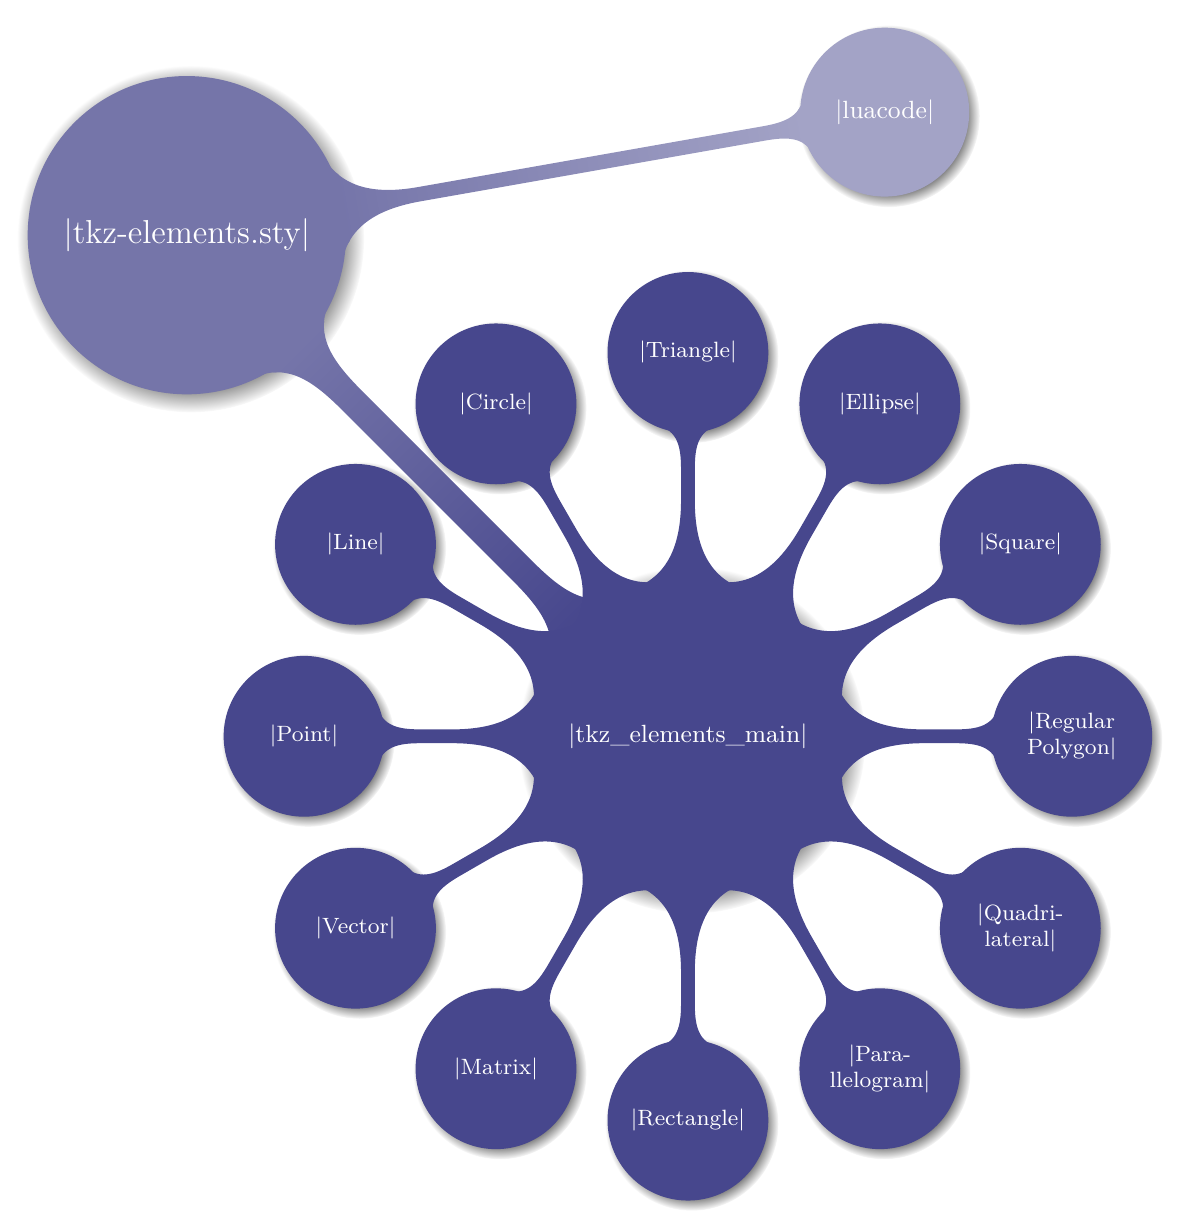
\begin{tikzpicture}[scale=.75]
\begin{scope}
\path[mindmap, concept color=MidnightBlue!60, text=white,text width=38mm,
 level 1 concept/.append style={level distance=120mm,
  sibling angle=72},
 set angles for level/.style={level 2/.append style={
 sibling angle=360/\the\tikznumberofchildren}},
 level/.append style={set angles for level=2},
 level 3 concept/.append style={level distance=20mm,
  sibling angle=20},
 L1/.style={level distance=45mm},
 L2/.style={level distance=65mm,minimum size=2cm}]

node[concept,circular drop shadow] {|tkz-elements.sty|} [clockwise from=10]
   child[concept color=MidnightBlue!40,minimum size=16mm] {
     node[concept,circular drop shadow] {|luacode|}
}
child[concept color= MidnightBlue!80,minimum size=4cm,text width=38mm,
clockwise from=27] { 
  node[concept,circular drop shadow] {|tkz\_elements\_main|} 
  [clockwise from=0]
  child[L2] { node[concept,circular drop shadow] {|Regular Polygon|} }
  child[L2] { node[concept,circular drop shadow] {|Quadri\-lateral|} }
  child[L2] { node[concept,circular drop shadow] {|Para\-llelogram|} }
  child[L2] { node[concept,circular drop shadow] {|Rectangle|} }
  child[L2] { node[concept,circular drop shadow] {|Matrix|} }
  child[L2] { node[concept,circular drop shadow] {|Vector|} }
  child[L2] { node[concept,circular drop shadow] {|Point|} }
  child[L2] { node[concept,circular drop shadow] {|Line|} }
  child[L2] { node[concept,circular drop shadow] {|Circle|} }
  child[L2] { node[concept,circular drop shadow] {|Triangle|} }
  child[L2] { node[concept,circular drop shadow] {|Ellipse|} }
  child[L2] { node[concept,circular drop shadow] {|Square|} }
};
\end{scope}
\end{tikzpicture}

The current classes are (some are still inactive):
\begin{itemize}
   \item active : \Iclass{point} (z) ;  \Iclass{line} (L) ; \Iclass{circle} (C) ; \Iclass{triangle} (T) ; \Iclass{ellipse} (E) ; \Iclass{quadrilateral} (Q) ; \Iclass{square} (S) ; \Iclass{rectangle} (R) ; \Iclass{parallelogram} (P) ; \Iclass{regular\_polygon} (RP); \Iclass{vector} (V).
   
   \item  inactive : matrix (M) ; vector (V).

\end{itemize}

If |name| is name of a class, you can find its definition in the file |tkz_elements_name.lua|.

     
% section structure (end)



\newpage
\section{Why tkz-elements?} % (fold)
\label{sec:why_tkz_elements}

\subsection{Calculation accuracy} % (fold)
\label{sub:calculation_accuracy}

\subsubsection{Calculation accuracy in \TIKZ} % (fold)
\label{ssub:calculation_accuracy_in_tikz}

With \TIKZ, \tkzimp{|veclen(x,y)|} calculates the expression $\sqrt{x^2+y^2}$.
This calculation is obtained using a polynomial approximation, based on ideas from \tkzimp{Rouben Rostamian}.

\pgfkeys{/pgf/number format/.cd,std,precision=5} \pgfmathparse{veclen(65,72)} 
\begin{mybox}{}
\begin{verbatim}
   pgfmathparse{veclen(65,72)} \pgfmathresult
\end{verbatim}
\end{mybox}

 \tkzHand $\sqrt{65^2+72^2} \approx \pmpn{\pgfmathresult} $ \tkzRBomb.
% subsubsection calculation_accuracy_in_tikz (end)

\subsubsection{Calculation accuracy in Lua} % (fold)
\label{ssub:calculation_accuracy_in_lua}

A |luaveclen| macro can be defined as follows:

\begin{mybox}{}
\begin{verbatim}
\def\luaveclen#1#2{\directlua{tex.print(string.format(
'\percentchar.5f',math.sqrt((#1)*(#1)+(#2)*(#2))))}}
\end{verbatim}
\end{mybox}

and

\begin{mybox}
\begin{verbatim}
\luaveclen{65}{72}
\end{verbatim}
\end{mybox}

gives 
\tkzHand $\sqrt{65^2+72^2} = \pmpn{\luaveclen{65}{72}} $ {\color{red}!!}

The error isn't important if it's a hundredth of a \tkzimp{pt} for the placement of an object on a page, but it's unpleasant for the result of a calculation in a mathematical demonstration. What's more, these inaccuracies can combine to produce erroneous constructions.

\vspace{.5em}
To remedy this lack of precision, I first introduced the package \pkg{fp}, then the package \pkg{xfp}. Lately, with the arrival of lua\LATEX{}, I have been able to add a \tkzname{Lua} option whose goal was to perform some calculations with \tkzname{Lua}.

This was the primary reason for creating the package, the second being the introduction of object-oriented programming and easier programming with Lua. Object-oriented programming (oop) convinced me to further develop all the possibilities this method offered.

At that moment, I had received some examples of programming with \tkzname{Lua} from {\tkzimpbf{Nicolas Kisselhoff}}, but I didn't understand its code, so I had to patiently study Lua. Finally, I was able to build tkz-elements,  I took many of his ideas I've adapted.


% subsubsection calculation_accuracy_in_lua (end)
\subsubsection{Using objects} % (fold)
\label{ssub:using_objects}

Then, I read an article\footnote{\href{https://www.guitex.org/home/images/meeting2012/slides/presentazione_giacomell_guitmeeting_2012.pdf}{Grafica ad oggetti con LuaTEX}} by \tkzimpbf{Roberto Giacomelli} on object programming based on the \tkzname{Lua} and \TIKZ\ tools. This was my second source of inspiration. Not only could the programming be done step-by-step, but the introduction of objects allowed the link between the code and the geometry. The code becomes more readable,  more explicit and better structured. 
 
\subsubsection{Example: Apollonius circle} % (fold)
\label{ssub:example_apollonius_circle}

\begin{mybox}{Problem}
The goal is to determine an inner tangent circle to the three exinscribed circles of a triangle. 
\end{mybox}

See \href{https://mathworld.wolfram.com/ApolloniusCircle.html}{MathWorld} for more details.

This example was my reference for testing the \pkg{tkz-euclide} package. With my first methods and the tools at my disposition, the results lacked precision. Now, with tkz-elements, I can use tools that are more powerful, more precise and easier to create.

The essential principles of figure construction with \tkzname{tkz-euclide} are kept: definitions, calculations, tracings, labels as well as the  step-by-step programmation, corresponding to a construction with a ruler and a compass.

This is the version that uses the simplest construction method, made possible by Lua.

\begin{mybox}
\begin{verbatim}
\begin{tkzelements}
  scale           = .4
  z.A             = point: new (0,0)
  z.B             = point: new (6,0)
  z.C             = point: new (0.8,4)
  T.ABC           = triangle : new ( z.A,z.B,z.C )
  z.N             = T.ABC.eulercenter
  z.S             = T.ABC.spiekercenter
  T.feuerbach     = T.ABC : feuerbach ()
  z.Ea,z.Eb,z.Ec  = get_points ( T.feuerbach )
  T.excentral     = T.ABC : excentral ()
  z.Ja,z.Jb,z.Jc  = get_points ( T.excentral )
  C.JaEa          = circle: new (z.Ja,z.Ea)
  C.ortho         = circle: radius (z.S,math.sqrt(C.JaEa: power(z.S)))
  z.a             = C.ortho.through
  C.euler         = T.ABC: euler_circle ()
  C.apo           = C.ortho : inversion (C.euler)
  z.O             = C.apo.center
  z.xa,z.xb,z.xc  = C.ortho : inversion (z.Ea,z.Eb,z.Ec)
\end{tkzelements}
\end{verbatim}
\end{mybox}

The creation of an object encapsulates its attributes (its characteristics) and methods (i.e. the actions that are specific to it). It is then assigned a reference (a name), which is linked to the object using a table. The table is an associative array that links the reference called \tkzimp{key} to a \tkzimp{value}, in this case the object. These notions will be developed later.

\tkzimp{T} is a table that associates the object \tkzimp{triangle} with the key \tkzimp{ABC}. \tkzimp{T.ABC} is also a table, and its elements are accessed using keys that are attributes of the triangle. These attributes have been defined in the package.

\vspace{1em}
\begin{mybox}
\begin{verbatim}
 z.N = T.ABC.eulercenter \end{verbatim}
\end{mybox}

|N| is the name of the point, |eulercenter| is an attribute of the triangle.
\footnote{ The center of the Euler circle, or center of the nine-point circle, is a characteristic of every triangle.}

\begin{mybox}
\begin{verbatim}
 T.excentral     = T.ABC : excentral () \end{verbatim}
\end{mybox}

Here, \tkzimp{excentral} is a method linked to the \tkzimp{T.ABC }object. It defines the triangle formed by the centers of the exinscribed circles. 

Two lines are important. The first below shows that the excellent precision provided by Lua makes it possible to define a radius with a complex calculation. The radius of the radical circle is given by $\sqrt{\Pi(S,\mathcal{C}(Ja,Ea))}$ (square root of the power of point $S$ with respect to the exinscribed circle with center |Ja| passing through |Ea|). 

\begin{mybox}
\begin{verbatim}
  C.ortho  = circle: radius (z.S,math.sqrt(C.JaEa: power(z.S)))\end{verbatim}
\end{mybox}

Finally, the inversion of the Euler circle with respect to the radical circle is the Apollonius circle\footnote{The nine-point circle, or Euler circle, is externally tangent to the three circles. The points of tangency form Feuerbach's triangle.}. The transformation has an object as parameter, which is recognized by its type (all objects are typed in the package), and the method determines which algorithm to use according to this type.

\begin{mybox}
\begin{verbatim}
  C.apo   = C.ortho : inversion (C.euler) \end{verbatim}
\end{mybox}

Now that all the points have been defined, it's time to start drawing the paths. To do this, you need to create the nodes. This is the role of the macro \Imacro{tkzGetNodes}. See \ref{ssub:points_transfer}

The following section concerns only drawings, and is handled by \pkg{tkz-euclide}.

\begin{verbatim}
\begin{tikzpicture}
   \tkzGetNodes
   \tkzFillCircles[green!30](O,xa)
   \tkzFillCircles[teal!30](Ja,Ea Jb,Eb Jc,Ec)
   \tkzFillCircles[lightgray](S,a)
   \tkzFillCircles[green!30](N,Ea)
   \tkzDrawPoints(xa,xb,xc)
   \tkzClipCircle(O,xa)
   \tkzDrawLines[add=3 and 3](A,B A,C B,C)
   \tkzDrawCircles(Ja,Ea Jb,Eb Jc,Ec S,a O,xa N,Ea)
   \tkzDrawPoints(O,A,B,C,S,Ea,Eb,Ec,N)
   \tkzDrawSegments[dashed](S,xa S,xb S,xc)
   \tkzLabelPoints(O,N,A,B)
   \tkzLabelPoints[right](S,C)
\end{tikzpicture}
\end{verbatim}

\vspace{1em}
\begin{tkzelements}
  scale           = .4
  z.A             = point: new (0,0)
  z.B             = point: new (6,0)
  z.C             = point: new (0.8,4)
  T.ABC           = triangle : new ( z.A,z.B,z.C )
  z.N             = T.ABC.eulercenter
  z.S             = T.ABC.spiekercenter
  T.feuerbach     = T.ABC : feuerbach ()
  z.Ea,z.Eb,z.Ec  = get_points ( T.feuerbach )
  T.excentral     = T.ABC : excentral ()
  z.Ja,z.Jb,z.Jc  = get_points ( T.excentral )
  C.JaEa          = circle: new (z.Ja,z.Ea)
  C.ortho         = circle: radius (z.S,math.sqrt(C.JaEa: power(z.S)))
  z.a             = C.ortho.through
  C.euler         = T.ABC: euler_circle ()
  C.apo           = C.ortho : inversion (C.euler)
  z.O             = C.apo.center
  z.xa,z.xb,z.xc  = C.ortho : inversion (z.Ea,z.Eb,z.Ec)
\end{tkzelements}
\begin{minipage}{\textwidth}
\hspace*{\fill}
\begin{tikzpicture}
   \tkzGetNodes
   \tkzFillCircles[green!30](O,xa)
   \tkzFillCircles[teal!30](Ja,Ea Jb,Eb Jc,Ec)
   \tkzFillCircles[lightgray](S,a)
   \tkzFillCircles[green!30](N,Ea)
   \tkzDrawPoints(xa,xb,xc)
   \tkzClipCircle(O,xa)
   \tkzDrawLines[add=3 and 3](A,B A,C B,C)
   \tkzDrawCircles(Ja,Ea Jb,Eb Jc,Ec S,a O,xa N,Ea)
   \tkzDrawPoints(O,A,B,C,S,Ea,Eb,Ec,N)
   \tkzDrawSegments[dashed](S,xa S,xb S,xc)
   \tkzLabelPoints(O,N,A,B)
   \tkzLabelPoints[right](S,C)
\end{tikzpicture}
\hspace*{\fill}  
\end{minipage}

% subsubsection example_apollonius_circle (end)
% subsubsection using_objects (end)
% subsection calculation_accuracy (end)
% section why_tkz_elements (end)
\newpage
\section{Presentation}

\subsection{With Lua} % (fold)
\label{sub:with_lua}

The purpose of tkz-elements is simply to calculate dimensions and define points. This is done in Lua. You can think of tkz-elements as a kernel that will be used either by tkz-euclide or by TikZ, see MetaPost.
Definitions and calculations are done inside the environment \tkzNameEnv{tkzelements}, this environment is based on \tkzNameEnv{luacode}.

\begin{minipage}[t]{.52\textwidth}\vspace{0pt}%
   The key points are: 
   \begin{itemize}
      \item the source file must be \tkzEHand\ {\color{red}\uline{ \color{black}utf8}}  encoded;
      \item compilation is done with \tkzEHand\ {\color{red}\uline{ \color{black}Lua\LATEX{}}};
      \item you need to load \tkzimp{\TIKZ}{} ou \tkzimp{tkz-euclide} and \tkzimp{tkz-elements};
      \item definitions and calculations are performed in an orthonormal sytem of reference, using Lua, and are carried out in an environment of  \tkzimp{tkzelements}.
   \end{itemize}
   
 To the right, see the minimum template.
  
The code is divided into two parts, which are two environments \tkzNameEnv{tkzelements} and \tkzNameEnv{tikzpicture}. In the first environment, you place your Lua code, and in the second, tkz-euclide commands.

\vspace*{4.1 cm}%
\end{minipage}\hspace*{\fill}
\begin{minipage}[t]{.45\textwidth}\vspace{0pt}%
\begin{mybox}
\begin{verbatim}
% !TEX TS-program = lualatex
% Created by Alain Matthes
\documentclass{standalone} 
\usepackage{tkz-euclide}
% or simply TikZ
\usepackage{tkz-elements}
begin{document} 
    
\begin{tkzelements}
   scale = 1
% definition of some points
z.A = point : new (   ,   )
z.B = point : new (   ,   )

 ...code...
\end{tkzelements}

\begin{tikzpicture}
% point transfer to Nodes
\tkzGetNodes

\end{tikzpicture}
\end{document}
\end{verbatim}
\end{mybox}
\end{minipage}
% subsection with_lua (end)

\subsection{The main process} % (fold)
\label{sub:the_main_process}

\tikzset{concept/.append style={fill={none}}}
\tikzset{root concept/.style=   {minimum size=3cm,text width=2.8cm}}%
\tikzset{level 1 concept/.append style={minimum size=4cm, font=\large, text width=3cm}}%
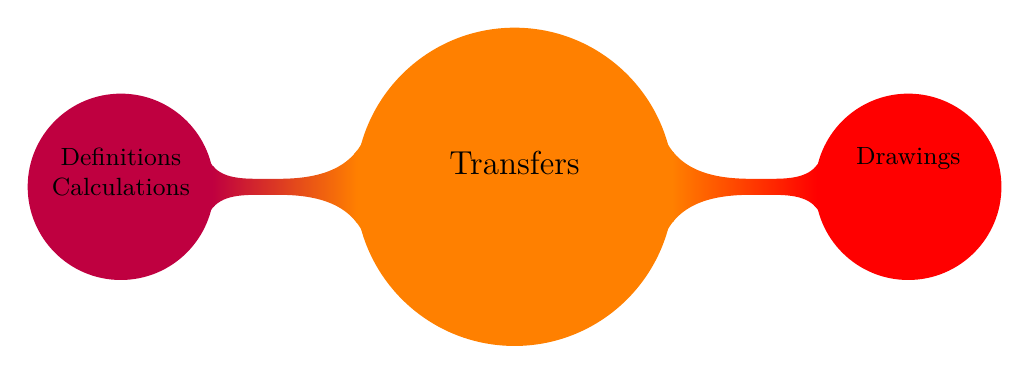
\begin{tikzpicture}
  \path[mindmap,concept color=orange,text=black]
    node[concept] {Transfers\\\textcolor{orange}{ \textbackslash{tkzGetNodes}}}
    child[concept color=red,grow=right] {
      node[concept] {Drawings\\\textcolor{red}{tkz-euclide}\\\textcolor{red}{\TIKZ}} }
    child[concept color=purple,grow=left] { 
    node[concept] {Definitions\\Calculations\\\textcolor{purple}{tkz-elements}} };
\end{tikzpicture}

When all the points necessary for the drawing are obtained, they must be transformed into \tkzname{nodes} so that \pkg{TikZ} or \pkg{tkz-euclide} can draw the figure. This is done through the macro \tkzcname{tkzGetNodes}. This macro browse all the elements of the table |z| using the key (in fact the name of the point) and retrieves the values associated with it, i.e. the coordinates of the point (node).
% subsection the_main_process (end)

\newpage
\subsection{Complete example: Pappus circle} % (fold)
\label{sub:the_figure_pappus_circle}

\subsubsection{The figure} 

\begin{tkzelements}
 scale = 1.2
  z.A  = point: new (0 , 0)
  z.B  = point: new (10 , 0)
  L.AB = line:  new ( z.A, z.B)
  z.C  = L.AB:  gold_ratio () 
  L.AC = line:  new ( z.A, z.C)
  L.CB = line:  new ( z.C, z.B)
  L.AB = line:  new ( z.A, z.B)
  z.O_0    = L.AB.mid
  z.O_1    = L.AC.mid
  z.O_2    = L.CB.mid
  C.AB = circle: new ( z.O_0, z.B) 
  C.AC = circle: new ( z.O_1, z.C) 
  C.CB = circle: new ( z.O_2, z.B)
  z.P  = C.CB.north  
  z.Q  = C.AC.north
  z.O  = C.AB.south
  z.c  = z.C : north (2)
  C.PC = circle: new ( z.P, z.C) 
  C.QA = circle: new ( z.Q, z.A)  
  z.P_0    = intersection (C.PC,C.AB)
  z.P_1    = intersection (C.PC,C.AC)
  _,z.P_2  = intersection (C.QA,C.CB)
  z.O_3 = triangle: new ( z.P_0, z.P_1, z.P_2).circumcenter
\end{tkzelements}
\hspace*{\fill}
   \begin{tikzpicture}
  \tkzGetNodes
  \tkzDrawCircle[black,fill=yellow!20,opacity=.4](O_0,B)
  \tkzDrawCircles[teal,fill=teal!40,opacity=.6](O_1,C O_2,B)
  \tkzDrawCircle[purple,fill=purple!20,opacity=.4](O_3,P_0)
  \tkzDrawArc[cyan,delta=10](Q,A)(P_0)
  \tkzDrawArc[cyan,delta=10](P,P_0)(B)
  \tkzDrawArc[cyan,delta=10](O,B)(A)
  \tkzDrawPoints(A,B,C,O_0,O_1,O_2,P,Q,P_0,P_0,P_1,P_2,O)
  \tkzLabelPoints(A,B,C,O_0,O_1,O_2,P,Q,P_0,P_0,P_1,P_2,O)
   \end{tikzpicture}
\hspace*{\fill}
% subsection the_figure_pappus_circle (end)

\subsubsection{The code} % (fold)
\label{ssub:the_code}

\begin{tkzexample}[small, code only,num]
% !TEX TS-program = lualatex
\documentclass{article}
\usepackage{tkz-euclide}
\usepackage{tkz-elements}
\begin{document}

\begin{tkzelements}
z.A     = point: new (0 , 0)
z.B     = point: new (10 , 0)        --  creation of two fixed points $A$ and $B$
L.AB    = line:  new ( z.A, z.B)
z.C     = L.AB:  gold_ratio ()       --  use of a method linked to “line”
z.O_0   = line:  new ( z.A, z.B).mid  -- midpoint of segment with an attribute of “line”
z.O_1   = line:  new ( z.A, z.C).mid --  objects are not stored and cannot be reused.
z.O_2   = line:  new ( z.C, z.B).mid   
C.AB    = circle: new ( z.O_0, z.B)  --  new object “circle” stored and reused
C.AC    = circle: new ( z.O_1, z.C) 
C.CB    = circle: new ( z.O_2, z.B)
z.P     = C.CB.north                 --  no“rth atrributes of a circle
z.Q     = C.AC.north
z.O     = C.AB.south
z.c     = z.C : north (2)           --   “north” method of a point (needs a parameter)
C.PC    = circle: new ( z.P, z.C) 
C.QA    = circle: new ( z.Q, z.A)  
z.P_0   = intersection (C.PC,C.AB)   --  search for intersections of two circles.
z.P_1   = intersection (C.PC,C.AC)  --   idem
_,z.P_2 = intersection (C.QA,C.CB)   --  idem
z.O_3   = triangle: new ( z.P_0, z.P_1, z.P_2).circumcenter -- circumcenter attribute of “triangle”
\end{tkzelements}

\begin{tikzpicture}
  \tkzGetNodes
  \tkzDrawCircle[black,fill=yellow!20,opacity=.4](O_0,B)
  \tkzDrawCircles[teal,fill=teal!40,opacity=.6](O_1,C O_2,B)
  \tkzDrawCircle[purple,fill=purple!20,opacity=.4](O_3,P_0)
  \tkzDrawArc[cyan,delta=10](Q,A)(P_0)
  \tkzDrawArc[cyan,delta=10](P,P_0)(B)
  \tkzDrawArc[cyan,delta=10](O,B)(A)
  \tkzDrawPoints(A,B,C,O_0,O_1,O_2,P,Q,P_0,P_0,P_1,P_2,O)
  \tkzLabelPoints(A,B,C,O_0,O_1,O_2,P,Q,P_0,P_0,P_1,P_2,O)
\end{tikzpicture}
\end{document}
\end{tkzexample}
% subsubsection the_code (end)

\subsection{Another example with comments: South Pole} % (fold)
\label{sub:south_pole}

Here's another example with comments

\begin{verbatim}
% !TEX TS-program = lualatex
\documentclass{standalone}
\usepackage{tkz-euclide,tkz-elements}
\begin{document}
\begin{tkzelements}                       
   z.A      = point: new (2 , 4)          -- we create environment tkzelements
   z.B      = point: new (0 , 0)          -- three fixed points are used
   z.C      = point: new (8 , 0)
   T.ABC    = triangle: new (z.A,z.B,z.C) -- we create a new triangle object
   C.ins    = T.ABC: in_circle ()         -- we get the incircle of this triangle
   z.I      = C.ins.center                -- center is an attribute of the circle
   z.T      = C.ins.through               -- through is also an attribute
   -- z.I,z.T  = get_points (C.ins)       -- get_points is a shortcut
   C.cir    = T.ABC : circum_circle ()    -- we get the  circumscribed circle
   z.W      = C.cir.center                -- we get the center of this circle   
   z.O      = C.cir.south                 -- now we get the south pole of this circle
   L.AO     = line: new (z.A,z.O)         -- we create an object "line"
   L.BC     = T.ABC.bc                    -- we get the line (BC)
   z.I_A    = intersection (L.AO,L.BC)    --  we search the intersection of the last lines
\end{tkzelements}
\end{verbatim}
\begin{tkzelements}
   scale    = 1.2
   z.A      = point: new (2 , 4)
   z.B      = point: new (0 , 0)
   z.C      = point: new (8 , 0)
   T.ABC    = triangle: new (z.A,z.B,z.C)
   C.ins    = T.ABC: in_circle ()
   z.I      = C.ins.center
   z.T      = C.ins.through
-- z.I,z.T  = get_points (C.ins)
   C.cir    = T.ABC : circum_circle ()
   z.W      = C.cir.center
   z.O      = C.cir.south
   L.AO     = line: new (z.A,z.O)
   L.BC     = T.ABC.bc
   z.I_A    = intersection (L.AO,L.BC)
\end{tkzelements}

\hspace*{\fill}
\begin{tikzpicture}
\tkzGetNodes
\tkzDrawCircles(W,A I,T)
\tkzDrawArc(O,C)(B)
\tkzDrawPolygon(A,B,C)
\tkzDrawSegments[new](A,O B,O C,O)
\tkzDrawLine(B,I)
\tkzDrawPoints(A,B,C,I,I_A,W,O)
\tkzFillAngles[green!20,opacity=.3](A,O,B A,C,B)
\tkzFillAngles[teal!20,opacity=.3](O,B,C B,C,O B,A,O O,A,C)
\tkzLabelPoints(I,I_A,W,B,C,O)
\tkzLabelPoints[above](A)
\end{tikzpicture}
\hspace*{\fill}

Here's the tikzpicture environment to obtain the drawing:
\begin{verbatim}
\begin{tikzpicture}
\tkzGetNodes
\tkzDrawCircles(W,A I,T)
\tkzDrawArc(O,C)(B)
\tkzDrawPolygon(A,B,C)
\tkzDrawSegments[new](A,O B,O C,O)
\tkzDrawLine(B,I)
\tkzDrawPoints(A,B,C,I,I_A,W,O)
\tkzFillAngles[green!20,opacity=.3](A,O,B A,C,B)
\tkzFillAngles[teal!20,opacity=.3](O,B,C B,C,O B,A,O O,A,C)
\tkzLabelPoints(I,I_A,W,B,C,O)
\tkzLabelPoints[above](A)
\end{tikzpicture}
\end{verbatim}
% subsection south_pole (end)
\endinput
\newpage

\section{Writing Convention} % (fold)
\label{sec:writing_convention}

\subsection{Miscellaneous} % (fold)
\label{sub:miscellanous}

\begin{itemize}
   \item Numerical variable: the writing conventions for real numbers are the same as for \pkg{Lua}.
   \item Complex numbers: Similar to real numbers, but to define them, you must write |za = point (1,2)|. Mathematically, this corresponds to 1+2i, which you can find with |tex.print(tostring(za))|.(Refer \ref{sub:complex_numbers})
   \item Boolean: you can write |bool = true| or |bool = false| then with Lua you can use the code :\\
 \begin{mybox}
|if bool == ... then ... else ... end|
\end{mybox}
 
 and outside the environment \tkzNameEnv{tkzelements} you can use the macro 
\begin{mybox}
 |\ifthenelse{\equal{\tkzUseLua{bool}}{true}}{ ... }{ ... }|
\end{mybox}

     after loading the \tkzNamePack{ifthen} package.
   
   \item String: if st = "Euler's formula" then \begin{mybox}
      |\tkzUseLua{st}| gives |Euler's formula|
   \end{mybox}
   

\end{itemize}
% subsection miscellanous (end)

\subsection{Assigning a Name to a Point} % (fold)
\label{sub:assigning_a_name_to_a_point}

At present,  the only obligation is to store the points in the table |z| \footnote{To place the point M in the table, simply write |z.M| = \ldots or |z["M"]|= \ldots} if you intend to use them in \TIKZ\ or \pkg{tkz-euclide}. f a point will not be used, you can designate it as you wish while adhering to Lua conventions. 

 Points within the  \tkzNameEnv{tkzelements} environment must follow a convention in the form |z.name|, where  |name| represents the name of the corresponding \tkzname{node}.
 
As for the conventions for designating |name| you must adhere to Lua conventions in particular cases.
\begin{enumerate}

   \item  The use of prime can be problematic. If the point name contains more than one symbol and ends with |p|  then when passing into \pkg{TikZ} or \pkg{tkz-euclide}, the letters |p|  will be replaced by |'| using the macro \tkzcname{tkzGetNodes}; \index{prime}

   \item  Alternatively, for a more explicit code, suppose you want to designate a point as  "euler". You could, for example,  write |euler = ...|, and at the end of the code for the transfer, |z.E = euler|. It is also possible to use a temporary name |euler| and to replace it in \TIKZ{}. Either at the time of placing the labels, or for example by using |pgfnodealias{E}{euler}|. This possibility also applies in other cases: prime, double prime, etc.
\end{enumerate}


Here are some different ways of naming a point:
\begin{mybox}
\begin{itemize}
   \item |z.A = point : new (1,2)|
   \item |z.Bp = point : new (3,4)|  --> this gives |B'| in the \tkzNameEnv{tikzpicture}
   \item |z.H_a = T.ABC : altitude ()| --> this gives |H_a| in the \tkzNameEnv{tikzpicture} code and $H_a$ in the display.
\end{itemize}
\end{mybox}
% subsection assigning_a_name_to_a_point (end)

\subsection{Assigning a Name to Other Objects} % (fold)
\label{sub:assigning_a_name_to_other_objects}

You have the flexibility to assign names to objects other than points. However, it's advisable to adhere to certain conventions to enhance code readability. For my examples, I've chosen the following conventions: first of all, I store the objects in tables: |L| for lines and segments, |C| for circles, |T| for triangles, |E| for ellipses.

\begin{itemize}
  \item 
  For lines, I use the names of the two points they pass through. For example, if a line passes through points  $A$ and $B$, I name the line |L.AB|. 

\item Circles are stored in table named |C|.
  For example, I name |C.AB| the circle of center $A$ passing through $B$. Other names like C.euler or C.external are also acceptable.

\item Triangles are stored in table named |T|.
  For example, I name |T.ABC| the triangle whose vertices are $A$, $B$ and $C$. However, names like |T.feuerbach| are also acceptable. 

\item Ellipses are stored in table named |E|.
  For ellipses, I name |E.ABC| the ellipse with center $A$ through vertex $B$ and covertex $C$.
\end{itemize}

Adhering to these conventions can help improve the readability of the code.

% subsection assigning_a_name_to_other_objects(end)

\subsection{Writing conventions for attributes, methods.} % (fold)
\label{sub:writing_conventions_for_attributes_methods_and_functions}

You must use the conventions of Lua, so

\begin{itemize}
   \item To obtain an \Amacro{attribute}, for all objects, the convention is identical: |object.attribute|. For example, for the point $A$ we access its abscissa with |z.A.re| and its ordinate with |z.A.im|; as for its type we obtain it with |z.A.type|. To get the south pole of the circle |C.OA| you need to write: |C.OA.south|.
   
   \item To use a method such as obtaining the incircle of a triangle ABC, just write  
   
   |C.incircle = T.ABC : in_circle ()|. 
   
   \item Some methods need a parameter. For example, to know the distance between a point  $C$  to the line $(A,B)$ we will write 
   
   |d = L.AB : distance (z.C)|.
   
   \item Use the \Amacro{underscore} to store a result you don't want to use. If you only need the second point of an intersection between a line and a circle, you would write 
   
   |_,z.J = intersection (L.AB , C.OC)|.

\end{itemize}
% section writing_convention (end)
\endinput
\section{Work organization} % (fold)
\label{sec:work_organization}

Here's a sample organization. 

The line |% !TEX TS-program = lualatex| ensures that you don't forget to compile with Lua\LATEX{}. The “standalone” class is useful, as all you need to do here is create a figure.


The package \pkg{ifthen} is useful if you need to use some Boolean.

The macro \tkzcname{LuaCodeDebugOn} allows you to try and find errors in Lua code.   

It is of course possible to leave the Lua code in the \tkzNameEnv{tkzelements} environment, but externalizing this code has its advantages. 

The first advantage, if you use a good editor, is to have a good presentation of the code. Styles are different between “Lua” and \LATEX{}. This makes the code clearer. This is how I proceeded, then reintegrated the code into the main code.

Another advantage is that you don't have to comment the code incorrectly. For Lua code, you comment lines with |--| (double minus sign), whereas for \LATEX{}, you comment with |%|.

Third advantage: the code can be reused.



\begin{verbatim}
% !TEX TS-program = lualatex
% Created by Alain Matthes on 2024-01-09.

\documentclass[margin = 12pt]{standalone} 
\usepackage{tkz-euclide}
\usepackage{tkz-elements,ifthen}

\begin{document} 
\LuaCodeDebugOn    
\begin{tkzelements}
 scale = 1.25
 dofile ("sangaku.lua")
\end{tkzelements}

\begin{tikzpicture}
   \tkzGetNodes
   \tkzDrawCircle(I,F)
   \tkzFillPolygon[color = purple](A,C,D)%
   \tkzFillPolygon[color = blue!50!black](A,B,C)%
   \tkzFillCircle[color = orange](I,F)%
\end{tikzpicture}
\end{document}
\end{verbatim}

And here is the code for the “Lua” part: the file |ex_sangaku.lua|

\begin{verbatim}
z.A         = point : new ( 0,0 ) 
z.B         = point : new ( 8,0 )
L.AB        = line : new ( z.A , z.B )
S           = L.AB : square ()
_,_,z.C,z.D = get_points (S)
z.F         = S.ac : projection (z.B)
L.BF        = line : new (z.B,z.F)
T.ABC       = triangle : new ( z.A , z.B , z.C )
L.bi        = T.ABC : bisector (2)
z.c         = L.bi.pb
L.Cc        = line : new (z.C,z.c)
z.I         = intersection (L.Cc,L.BF)
\end{verbatim}

\begin{tkzelements}
 scale = 1.25
 dofile ("sangaku.lua")
\end{tkzelements}

\begin{tikzpicture}
   \tkzGetNodes
   \tkzDrawCircle(I,F)
   \tkzFillPolygon[color = purple](A,C,D)%
   \tkzFillPolygon[color = blue!50!black](A,B,C)%
   \tkzFillCircle[color = orange](I,F)%
\end{tikzpicture}

\subsection{Scale problem} % (fold)
\label{sub:scale_problem}

If necessary, it's better to do the scaling in the “Lua” section. The reason is that it will be more accurate. There is, however, a problem to be aware of. I've made it a point of honor to avoid using numerical values in my codes whenever possible. In principle, these values only appear in the definition of fixed points. If the “scale” option is used, scaling is applied when points are created. Let's imagine you want to organize your code as follows:

|scale = 1.5|\\
|xB = 8|\\
|z.B         = point : new ( xB,0 )|

Scaling would then be ineffective, as the numerical values are not modified, only the point coordinates. To take scaling into account, use the function \Igfct{math}{value (v) }.

|scale = 1.5|\\
|xB = value (8)|\\
|z.B         = point : new ( xB,0 )|

\subsection{Code presentation} % (fold)
\label{sub:code_presentation}

The key point is that, unlike \LATEX{} or \TEX{}, you can insert spaces absolutely anywhere. 
% subsection code_presentation (end)
% subsection scale_problem (end)
% section work_organization (end)

\newpage
\section{Transfers} % (fold)
\label{sec:transfers}
\subsection{Fom Lua to tkz-euclide or TikZ} % (fold)
\label{sub:fom_lua_to_tkz_euclide_or_tikz}

In this section, we'll look at how to transfer points, Booleans and numerical values.

\subsubsection{Points transfer} % (fold)
\label{ssub:points_transfer}
We use an environment \tkzname{tkzelements}  outside an environment \tkzname{tikzpicture} which allows us to carry out all the necessary calculations, then we launch the macro \Imacro{tkzGetNodes} which transforms the affixes of the table \tkzname{z} into  \tkzname{Nodes}. It only remains to draw.

Currently the drawing program is either \TIKZ\ or \pkg{tkz-euclide}. You have the possibility to use another package to trace but for that you have to create a macro similar to \tkzcname{tkzGetNodes}. Of course, this package must be able to store the points as does \TIKZ\ or \pkg{tkz-euclide}. 

\vspace*{1em}

\begin{mybox}
\begin{verbatim}
\def\tkzGetNodes{\directlua{%
   for K,V in pairs(z) do
      local n,sd,ft
      n = string.len(K)
      if n >1 then
      _,_,ft, sd = string.find( K , "(.+)(.)" )  
     if sd == "p" then   K=ft.."'" end 
     _,_,xft, xsd = string.find( ft , "(.+)(.)" ) 
     if xsd == "p" then  K=xft.."'".."'" end 
       end    
  tex.print("\\coordinate ("..K..") at ("..V.re..","..V.im..") ;\\\\")
end}
}
\end{verbatim}
\end{mybox}
See the section In-depth Study \ref{sec:in_depth_study} for an explanation of the previous code.

The environment \tkzNameEnv{tkzelements} allows to use the underscore |_| and the macro \tkzcname{tkzGetNodes} allows to obtain names of nodes containing \tkzname{prime} or \tkzname{double prime}. (see the next example)

\begin{minipage}{0.5\textwidth}
\begin{verbatim}
\begin{tkzelements}
   scale = 1.2
   z.o   = point: new (0,0)
   z.a_1 = point: new (2,1)
   z.a_2 = point: new (1,2)
   z.ap  = z.a_1 + z.a_2
   z.app = z.a_1 - z.a_2
\end{tkzelements}
\begin{tikzpicture}
   \tkzGetNodes
   \tkzDrawSegments(o,a_1 o,a_2 o,a' o,a'')
   \tkzDrawSegments[red](a_1,a' a_2,a')
   \tkzDrawSegments[blue](a_1,a'' a_2,a'')
   \tkzDrawPoints(a_1,a_2,a',o,a'')
   \tkzLabelPoints(o,a_1,a_2,a',a'')
\end{tikzpicture}
\end{verbatim}
\end{minipage}
\begin{minipage}{0.5\textwidth}
\begin{tkzelements}
   scale = 1.2
   z.o   = point: new (0,0)
   z.a_1 = point: new (2,1)
   z.a_2 = point: new (1,2)
   z.ap  = z.a_1 + z.a_2
   z.app = z.a_1 - z.a_2
\end{tkzelements}
\hspace{\fill}
\begin{tikzpicture}
   \tkzGetNodes
   \tkzDrawSegments(o,a_1 o,a_2 o,a' o,a'')
   \tkzDrawSegments[red](a_1,a' a_2,a')
   \tkzDrawSegments[blue](a_1,a'' a_2,a'')
   \tkzDrawPoints(a_1,a_2,a',o,a'')
   \tkzLabelPoints(o,a_1,a_2,a',a'')
\end{tikzpicture}
\hspace{\fill}
\end{minipage}%

\newpage
% subsection fom_lua_to_tkz_euclide_or_tikz (end)
\subsubsection{Other transfers} % (fold)
\label{ssub:other_transfers}

Sometimes it's useful to transfer angle, length measurements or boolean. For this purpose, I have created the macro (see \ref{sub:transfer_from_lua_to_tex})  
\IEmacro{tkzUseLua(value)}

\begin{verbatim}
\begin{tkzelements}
   z.b = point:  new (1,1)
   z.a = point:  new (4,2)
   z.c = point:  new (2,2)
   z.d = point:  new (5,2)
   L.ab = line : new (z.a,z.b)
   L.cd = line : new (z.c,z.d)
    det = (z.b-z.a)^(z.d-z.c)
    if det == 0 then bool = true 
      else bool = false
    end
    x = intersection (L.ab,L.cd)
\end{tkzelements}

The intersection of the two lines lies at
    a point whose affix is:\tkzUseLua{x}

\begin{tikzpicture}
   \tkzGetNodes
    \tkzDrawPoints(a,...,d)
    \ifthenelse{\equal{\tkzUseLua{bool}}{true}}{
    \tkzDrawSegments[red](a,b c,d)}{%
    \tkzDrawSegments[blue](a,b c,d)}
     \tkzLabelPoints(a,...,d)
\end{tikzpicture}
\end{verbatim}

   \begin{tkzelements}
   z.b = point:  new (1,1)
   z.a = point:  new (4,2)
   z.c = point:  new (2,2)
   z.d = point:  new (5,1)
   L.ab = line : new (z.a,z.b)
   L.cd = line : new (z.c,z.d)
    det = (z.b-z.a)^(z.d-z.c)
    if det == 0 then bool = true 
      else bool = false
    end
    x = intersection (L.ab,L.cd)
   \end{tkzelements}

   The intersection of the two lines lies at
    a point whose affix is: \tkzUseLua{x}

\vspace{1em}
\hspace{\fill}
\begin{tikzpicture}
      \tkzGetNodes
      \tkzInit[xmin =-1,ymin=-1,xmax=6,ymax=3]
      \tkzGrid\tkzAxeX\tkzAxeY
       \tkzDrawPoints(a,...,d)
       \ifthenelse{\equal{\tkzUseLua{bool}}{true}}{
       \tkzDrawSegments[red](a,b c,d)}{%
       \tkzDrawSegments[blue](a,b c,d)}
       \tkzLabelPoints(a,...,d)
   \end{tikzpicture}
   \hspace{\fill} 
% subsubsection other_transfers (end)
% subsubsection points_transfer (end)
% section transferts (end)

\endinput
\newpage

\section{Class and object} % (fold)
\label{sec:class_and_object}

\subsection{Class} % (fold)
\label{sub:class}

 Object-oriented programming (OOP) is defined as a programming model built on the concept of objects. An object can be defined as a data table that has unique attributes and methods (operations) that define its behavior.
 
 \vspace{1em}
A class is essentially a user-defined data type. It describes the contents of the objects that belong to it. A class is a  blueprint of an object, providing initial values for   attributes and implementations of methods\footnote{action which an object is able to perform.} common to all objects of a certain kind.
% subsection class (end)

\subsection{Object} % (fold)
\label{sub:object}
 An Object is an instance of a class. Each object contains attributes and methods. Attributes are information or object characteristics stored in the date table (called field). The methods define behavior.
 
  \vspace{1em}
 All objects in the package are typed. The object types currently defined and used are: \tkzNameObj{point}, \tkzNameObj{line}, \tkzNameObj{circle}, \tkzNameObj{triangle}, \tkzNameObj{ellipse}, \tkzNameObj{quadrilateral}, \tkzNameObj{square}, \tkzNameObj{rectangle}, \tkzNameObj{parallelogram} and \tkzNameObj{regular\_polygon}. 

They can be created directly using the method \Imeth{obj}{new} by giving points, with the exception of the \Iclass{class}{point} class which requires a pair of reals, and \Iclass{class}{regular\_polygon} which needs two points and an integer.

 Objects can also be obtained by applying methods to other objects. For example, |T.ABC : circum_circle ()| creates an object \tkzNameObj{circle}. Some object attributes are also objects, such as |T.ABC.bc| which creates the object \tkzNameObj{line}, a straight line passing through the last two points defining the triangle.

 \vspace{1em}

 \subsubsection{Attributes} % (fold)
 \label{ssub:attributes}
 Attributes are accessed using the classic method, so |T.pc| gives the third point  of the triangle and |C.OH.center| gives the center of the circle, but I've added a |get_points| function that returns the points of an object. This applies to straight lines (pa and pc), triangles (pa, pb and pc) and circles (center and through).

  \vspace{1em}
  Example: |z.O,z.T = get_points (C)| recovers the center and a point of the circle.
 % subsubsection attributes (end)

\subsubsection{Methods} % (fold)
\label{ssub:methods}

A method is an operation (function or procedure) associated (linked) with an object.

Example:   The point object is used to vertically determine a new point object located at a certain distance from it (here 2). Then it is possible to rotate objects around it.

\begin{verbatim}
   \begin{tkzelements}
      z.A = point (1,0)
      z.B = z.A : north (2)             
      z.C = z.A : rotation (math.pi/3,z.B)
      tex.print(tostring(z.C))
   \end{tkzelements}
\end{verbatim}

\begin{tkzelements}
   z.A = point (1,0)
   z.B = z.A : north (2)
   z.C = z.A : rotation (math.pi/3,z.B)
   tex.print(tostring("The coordinates of $C$ are: " .. z.C.re .." and "..z.C.im))
\end{tkzelements}


% subsubsection methods (end)
% subsection object (end)
% section class_and_object (end)
\endinput
\newpage

\section{Class \Iclass{point}} % (fold)
\label{sec:class_point}

The class on which the whole edifice rests,  it's the class \Iclass{point}. This class is hybrid in the sense that it is as much about points of a plane as complex numbers. The principle is the following: the plane is provided with an orthonormal basis which allows us to determine the placement of a point using its abscissa and ordinate coordinates; in the same way any complex number can simply be considered as a pair of real numbers (its real part and its imaginary part). We can then designate the plane as the complex plane, and the complex number $x+iy$ is represented by the point of the plane with coordinates $(x,y)$. Thus the point $A$ will have coordinates stored in the object $z.A$. Coordinates are attributes of the "point" object, like type, argument and modulus.



The creation of a point is done using the following method, but there are other possibilities. If a scaling factor has been given, the method takes it into account.

   \def\size{42mm}
\begin{tikzpicture}[remember picture]
\node[ draw, fill=red!10] (tbl) {%
 \centering
\begin{minipage}{\size}

   \hspace{\fill} \texttt{Arguments}\hspace{\fill}
       
       \tikz\node[minimum width=\size,font=\small,
    draw, fill=cyan!10,
    rectangle split, rectangle split parts=5
  ] {
    \texttt{re (real)}
    \nodepart{two}\texttt{im (real)}
    \nodepart{three}\texttt{type = 'point'}
    \nodepart{four}\texttt{argument (rad)}
     \nodepart{five}\texttt{modulus (cm)}
  };
  
    \hspace{\fill}  \texttt{Methods}\hspace{\fill}
    
        \tikz\node[minimum width=\size,font=\small,
    draw, fill=orange!20,sharp corners,
    rectangle split, rectangle split parts=4
  ] {
   \texttt{homothety(coeff,obj)}
    \nodepart{two}\texttt{rotation (angle,object)}
    \nodepart{three}\texttt{symmetry (object)}
    \nodepart{four}\texttt{\ldots}
  };
\end{minipage}};
 \node[ draw, fill=red!10,,minimum height = 2em,
  rounded corners,anchor=south] (tc) at (tbl.north){Class |Point|};
\end{tikzpicture}
\hspace{5cm}\begin{tikzpicture}[remember picture]
   \node[ draw, fill=red!10] (tbl) {%
 \centering
\begin{minipage}{\size}
   \hspace{\fill}    \texttt{Arguments}\hspace{\fill}
       
        \tikz\node[minimum width=\size,font=\small,
    draw, fill=cyan!10,
    rectangle split, rectangle split parts=5
  ] {
    \texttt{re = 1}
    \nodepart{two}\texttt{im = 2}
    \nodepart{three}\texttt{type = 'point'}
    \nodepart{four}\texttt{argument = atan(2)}
     \nodepart{five}\texttt{modulus = $\sqrt{5}$}
  };
  
    \hspace{\fill}  \texttt{Methods}\hspace{\fill}
    
        \tikz\node[minimum width=\size,font=\small,
    draw, fill=orange!20,sharp corners,
    rectangle split, rectangle split parts=4
  ] {
   \texttt{homothety(coeff,obj)}
    \nodepart{two}\texttt{rotation (angle,object)}
    \nodepart{three}\texttt{symmetry (object)}
    \nodepart{four}\texttt{\ldots}
  };
\end{minipage}
     };
 \node[ draw, fill=red!10,remember picture,minimum height = 2em,
  rounded corners,anchor=south] (to) at (tbl.north){object |z.A|};
\end{tikzpicture}

\begin{tikzpicture}[remember picture,overlay]
\draw [thick,->](tc.east) -- (to.west);
\end{tikzpicture}

\subsection{Attributes of a point} % (fold)
\label{sub:attributes_of_a_point}
% Method \Imeth{point}{new}

\begin{mybox}
   Creation |z.A = point: new (1,2) |
\end{mybox}
 The point $A$ has coordinates $x=1$ and $y=2$. If you use the notation |z.A| then $A$ will be the reference of a node in \TIKZ\ or in \pkg{tkz-euclide}.

This is the creation of a fixed point with coordinates 1 and 2 and which is named $A$. The notation |z.A| indicates that the coordinates will be stored in a table noted |z| (reference to the notation of the affixes of the complex numbers) that A is the name of the point and the key allowing access to the values. 


\vspace{1em}
\bgroup
\small
\catcode`_=12
\captionof{table}{Point attributes.}\label{point:att}  
\begin{tabular}{lll}
\toprule
\textbf{Attributes}     & \textbf{Application}& \textbf{Example}\\
\Iattr{point}{re}       &  |z.A.re = 1|    & see (\ref{ssub:methods}) \\
\Iattr{point}{im}       &  |z.A.im = 2|    &see (\ref{ssub:methods})  \\
\Iattr{point}{type}     &  |z.A.type = 'point'|  & \\  
\Iattr{point}{argument} &  |z.A.argument $\approx$ 0.78539816339745| & see (\ref{ssub:example_point_attributes})\\
\Iattr{point}{modulus}   & |z.A.modulus| $\approx$ |2.2360...| =$\sqrt{5}$ & see (\ref{ssub:example_point_attributes})\\
\bottomrule
\end{tabular}
\egroup

\newpage
\subsubsection{Example:point attributes} % (fold)
\label{ssub:example_point_attributes}

\begin{tkzelements}
   z.M = point: new (1,2)
\end{tkzelements}
\hspace*{\fill}


\begin{verbatim}
\begin{tkzelements}
   z.M = point: new (1,2)
\end{tkzelements}
\end{verbatim}
\pgfkeys{/pgf/number format/.cd,std,precision=2}
\let\pmpn\pgfmathprintnumber
\DeleteShortVerb{\|}

\begin{verbatim}
\begin{tikzpicture}[scale = 1]
\pgfkeys{/pgf/number format/.cd,std,precision=2}
\let\pmpn\pgfmathprintnumber
\tkzDefPoints{2/4/M,2/0/A,0/0/O,0/4/B}
\tkzLabelPoints(O)
\tkzMarkAngle[fill=gray!30,size=1](A,O,M)
\tkzLabelAngle[pos=1,right](A,O,M){%
$\theta \approx \pmpn{\tkzUseLua{z.M.argument}}$ rad}
\tkzDrawSegments(O,M)
\tkzLabelSegment[above,sloped](O,M){%
$|z_M| =\sqrt{5}\approx \pmpn{\tkzUseLua{z.M.modulus}}$ cm}
\tkzLabelPoint[right](M){$M : z_M = 1 + 2i$}
\tkzDrawPoints(M,A,O,B)
\tkzPointShowCoord(M)
\tkzLabelPoint[below,teal](A){$\tkzUseLua{z.M.re}$}
\tkzLabelPoint[left,teal](B){$\tkzUseLua{z.M.im}$}
\tkzDrawSegments[->,add = 0 and 0.25](O,B O,A)
\end{tikzpicture}
\end{verbatim}


\begin{center}
   \begin{tikzpicture}
   \pgfkeys{/pgf/number format/.cd,std,precision=2}
   \let\pmpn\pgfmathprintnumber
   \tkzDefPoints{2/4/M,2/0/A,0/0/O,0/4/B}
   \tkzLabelPoints(O)
   \tkzMarkAngle[fill=gray!30,size=1](A,O,M)
   \tkzLabelAngle[pos=1,right](A,O,M){%
   $\theta \approx \pmpn{\tkzUseLua{z.M.argument}}$ rad}
   \tkzDrawSegments(O,M)
   \tkzLabelSegment[above,sloped](O,M){%
   $|z_M| =\sqrt{5}\approx \pmpn{\tkzUseLua{z.M.modulus}}$ cm}
   \tkzLabelPoint[right](M){$M : z_M = 1 + 2i$}
   \tkzDrawPoints(M,A,O,B)
   \tkzPointShowCoord(M)
   \tkzLabelPoint[below,teal](A){$\tkzUseLua{z.M.re}$}
   \tkzLabelPoint[left,teal](B){$\tkzUseLua{z.M.im}$}
   \tkzDrawSegments[->,add = 0 and 0.25](O,B O,A)
   \begin{scope}[every annotation/.style={fill=lightgray!15,anchor = east}]
   \node [annotation,font =\small,text width=6cm] at (current bounding box.west) {
Attributes of \texttt{z.M}
   \begin{itemize}
   \item \texttt{z.M.re} = 1
   \item \texttt{z.M.im} = 2
   \item \texttt{z.M.type} = 'point'
   \item \texttt{z.M.argument} = $\theta \approx \pmpn{\tkzUseLua{z.M.argument}}$ rad
   \item \texttt{z.M.modulus} = $|z_M| =\sqrt{5}\approx \pmpn{\tkzUseLua{z.M.modulus}}$ cm
   \end{itemize}
       };
   \end{scope}
   \end{tikzpicture}
\end{center}

 \MakeShortVerb{\|}
    \hspace*{\fill}
 %  \caption{Class Point}
% subsubsection example_point_attributes (end)
% subsection attributes_of_a_point (end)

\subsubsection{Argand diagram} % (fold)
\label{ssub:argand_diagram}
\normalsize
\begin{minipage}{\textwidth}
   \begin{verbatim}
   \begin{tkzelements}
      z.A = point : new ( 2 , 3 )
      z.O = point : new ( 0 , 0 )
      z.I = point : new ( 1 , 0 )
   \end{tkzelements}
   \hspace{\fill}\begin{tikzpicture}
      \tkzGetNodes
      \tkzInit[xmin=-4,ymin=-4,xmax=4,ymax=4]
      \tkzDrawCircle[dashed,red](O,A)
      \tkzPointShowCoord(A)
      \tkzDrawPoint(A)
      \tkzLabelPoint[above right](A){\normalsize $a+ib$}
      \tkzDrawX\tkzDrawY
      \tkzDrawSegment(O,A)
      \tkzLabelSegment[above,anchor=south,sloped](O,A){ OA = modulus of $z_A$}
     \tkzLabelAngle[anchor=west,pos=.5](I,O,A){$\theta$ = argument of $z_A$}
   \end{tikzpicture}
   \end{verbatim}
\end{minipage}

\begin{minipage}{\textwidth}
   \begin{tkzelements}
      z.A = point : new ( 2 , 3 )
      z.O = point : new ( 0 , 0 )
      z.I = point : new ( 1 , 0 )
   \end{tkzelements}
   \hspace{\fill}\begin{tikzpicture}
      \tkzGetNodes
      \tkzInit[xmin=-4,ymin=-4,xmax=4,ymax=4]
      \tkzDrawCircle[dashed,red](O,A)
      \tkzPointShowCoord(A)
      \tkzDrawPoint(A)
      \tkzLabelPoint[above right](A){\normalsize $a+ib$}
      \tkzDrawX\tkzDrawY
      \tkzDrawSegment(O,A)
      \tkzLabelSegment[above,anchor=south,sloped](O,A){ OA = modulus of $z_A$}
     \tkzLabelAngle[anchor=west,pos=.5](I,O,A){$\theta$ = argument of $z_A$}
   \end{tikzpicture}
   \hspace{\fill}
\end{minipage}


% subsubsection argand_diagram (end)
\newpage
\subsection{Methods of the class point} % (fold)
\label{sub:methods_of_the_class_point}

The methods described in the following table are standard. You'll find them in most of the examples at the end of this documentation. The result of the different methods presented in the following table is a \tkzNameObj{point}. See section  (\ref{sub:complex_numbers}) for the metamethods.

\vspace{1em}
\bgroup
\catcode`_=12
\small
\captionof{table}{Methods of the class point.}\label{point:met}
\begin{tabular}{lll}
\toprule
\textbf{Methods} & \textbf{Application}& \\
\midrule
\Imeth{point}{new(r, r)}    & |z.A = point : new(1,2)| & see (\ref{ssub:method_normalize}) \\
\Imeth{point}{polar (d, an)}  & |z.A = point : polar(1,math.pi/3)| &  see (\ref{sub:archimedes} )\\
\Imeth{point}{polar\_deg an} &    an in deg    &  polar coordinates an deg \\
\midrule
\textbf{Points} &&\\
\midrule
\Imeth{point}{north(r)} & |r| distance to the point (1 if empty) & see (\ref{sub:power_v2}) ; \ref{ssub:methods})   \\
\Imeth{point}{south(r)} & &  \\
\Imeth{point}{east(r)}  &  & \\
\Imeth{point}{west(r)}  &  & \\
\Imeth{point}{normalize()} &  |z.b = z.a: normalize ()| &  see (\ref{ssub:method_normalize}) \\
\Imeth{point}{get\_points (obj)}     & retrieves points from the object &    \\
\Imeth{point}{orthogonal (d)} & |z.B=z.A:orthogonal(d)| &  $\overrightarrow{OB}\perp \overrightarrow{OA}$  and $OB=d$\\
\Imeth{point}{at ()} & |z.X = z.B : at (z.A)| &  $\overrightarrow{OB}= \overrightarrow{AX}$  and $OB=d$\\
 \midrule
  \textbf{Transformations} &&\\
 \midrule
  \Imeth{point}{symmetry(obj)} & obj : point, line, etc. & see (\ref{ssub:object_symmetry}) \\
 \Imeth{point}{rotation(an , obj)}  & point, line, etc.  &  see (\ref{ssub:object_rotation})\\
  \Imeth{point}{homothety(r,obj)}     & |z.c = z.a : homothety (2,z.b)| & see (\ref{sub:homothety})   \\
\bottomrule %
\end{tabular}
\egroup

\subsubsection{Example: method \Imeth{point}{north (d)} } % (fold)
\label{ssub:example_method_imeth_point_north_d}

This function defines a point located on a vertical line passing through the given point. This function is useful if you want to report a certain distance (see the following example).
If |d| is absent then it is considered equal to 1.

\begin{minipage}{.5\textwidth}
\begin{verbatim}
\begin{tkzelements}
   z.O   = point : new ( 0, 0 )
   z.A   = z.O : east ()
   z.Ap  = z.O : east (2) : north (2)
   z.B   = z.O : north ()
   z.C   = z.O : west ()
   z.D   = z.O : south ()
\end{tkzelements}
\begin{tikzpicture}
   \tkzGetNodes
   \tkzDrawPolygon(A,B,C,D)
   \tkzDrawPoints(A,B,C,D,O,A')
\end{tikzpicture}
\end{verbatim}
\end{minipage}
\begin{minipage}{.5\textwidth}
\begin{tkzelements}
   scale = 1.5
   z.O = point : new ( 0, 0 )
   z.A = z.O : east ()
   z.Ap = z.O : east (2) : north (2)
   z.B = z.O : north ()
   z.C = z.O : west ()
   z.D = z.O : south ()
\end{tkzelements}
\hspace{\fill}
\begin{tikzpicture}
   \tkzGetNodes
   \tkzDrawPolygon(A,B,C,D)
   \tkzDrawPoints(A,B,C,D,O,A')
   \tkzLabelPoints(A,B,C,D,O,A')
\end{tikzpicture}
\end{minipage}
% subsubsection example_method_imeth_point_north_d (end)


\subsubsection{Length transfer} % (fold)
\label{ssub:report_de_distance}

Use of |north and east| functions linked to points, to transfer lengths, see (\ref{sub:length_of_a_segment})

\begin{minipage}{.4\textwidth}
\begin{verbatim}
\begin{tkzelements}
   z.A = point : new ( 0 , 0 )
   z.B = point : new ( 3 , 0 )
   L.AB = line : new ( z.A , z.B )
   T.ABC =   L.AB : sublime ()
   z.C = T.ABC.pc
   z.D = z.B: north (length(z.B,z.C))
   z.E = z.B: east (L.AB.length)
   z.M = L.AB.mid
   z.F = z.E : north (length(z.C,z.M))
\end{tkzelements}
\begin{tikzpicture}[gridded]
   \tkzGetNodes
   \tkzDrawPolygons(A,B,C) 
   \tkzDrawSegments[gray,dashed](B,D B,E E,F C,M)
   \tkzDrawPoints(A,...,F)
   \tkzLabelPoints(A,B,E,M)
   \tkzLabelPoints[above right](C,D,F)
\end{tikzpicture}
\end{verbatim}
\end{minipage}
\begin{minipage}{.6\textwidth}
\begin{tkzelements}
   z.A = point : new ( 0 , 0 )
   z.B = point : new ( 3 , 0 )
   L.AB = line : new ( z.A , z.B )
   T.ABC =   L.AB : sublime ()
   z.C = T.ABC.pc
   z.D = z.B: north (length(z.B,z.C))
   z.E = z.B: east (L.AB.length)
   z.M = L.AB.mid
   z.F = z.E : north (length(z.C,z.M))
\end{tkzelements}
\hspace{\fill}
\begin{tikzpicture}[gridded]
   \tkzGetNodes
   \tkzDrawPolygons(A,B,C) 
   \tkzDrawSegments[gray,dashed](B,D B,E E,F C,M)
   \tkzDrawPoints(A,...,F)
   \tkzLabelPoints(A,B,E,M)
   \tkzLabelPoints[above right](C,D,F)
\end{tikzpicture}
\end{minipage}
% subsubsection report_de_distance (end)


\subsubsection{Example: method \Imeth{point}{polar} } % (fold)
\label{ssub:example_polar_method}

This involves defining a point using its modulus and argument.

\begin{minipage}{0.6\textwidth}
\begin{tkzexample}[latex=0cm,small,code only]
\begin{tkzelements}
   z.O     = point:   new  (0, 0)
   z.A     = point:   new  (3, 0)
   z.F     = point:   polar (3, math.pi/3)
\end{tkzelements}
\begin{tikzpicture}
   \tkzGetNodes
   \tkzDrawCircle(O,A)
   \tkzDrawSegments[new](O,A)
   \tkzDrawSegments[purple](O,F)
   \tkzDrawPoints(A,O,F)
   \tkzLabelPoints[below right=6pt](A,O,F)
\end{tikzpicture}
\end{tkzexample}
\end{minipage}
\begin{minipage}{0.4\textwidth}
\begin{tkzelements}
    scale   = .75
    z.O     = point:   new  (0, 0)
    z.A     = point:   new  (3, 0)
    z.F     = point:   polar (3, math.pi/3)
\end{tkzelements}
\hspace*{\fill}
\begin{tikzpicture}
\tkzGetNodes
\tkzDrawCircle(O,A)
\tkzDrawSegments[new](O,A)
\tkzDrawSegments[purple](O,F)
\tkzDrawPoints(A,O,F)
\tkzLabelPoints(A,O,F)
\end{tikzpicture}
\hspace*{\fill}
\end{minipage}
% subsubsection example_polar_method (end)

\subsubsection{Method \Imeth{point}{normalize ()}} % (fold)
\label{ssub:method_normalize}

The result is a point located between the origin and the initial point at a distance of $1$ from the origin.

\begin{minipage}{.4\textwidth}
\begin{verbatim}
\begin{tkzelements}
   scale = 1.5
   z.O = point : new (0,0)
   z.A = point : new (1,2)
   z.B = z.A : normalize ()
   z.I = point : new (1,0)
\end{tkzelements}
\begin{tikzpicture}
   \tkzGetNodes
   \tkzDrawSegment(O,A)
   \tkzDrawCircle(O,B)
   \tkzDrawPoints(O,A,B,I)
   \tkzLabelPoints(O,A,B)
   \tkzLabelPoint[below right](I){$1$}
\end{tikzpicture}
\end{verbatim}
\end{minipage}
\begin{minipage}{.6\textwidth}
\begin{tkzelements}
scale = 1.5
z.O = point : new (0,0)
z.A = point : new (1,2)
z.B = z.A : normalize ()
z.I = point : new (1,0)
\end{tkzelements}
 \hspace*{\fill}
\begin{tikzpicture}
\tkzGetNodes
\tkzDrawSegment(O,A)
\tkzDrawCircle(O,B)
\tkzDrawPoints(O,A,B,I)
\tkzLabelPoints(O,A,B)
\tkzLabelPoint[below right](I){$1$}
\end{tikzpicture}
 \hspace*{\fill}
\end{minipage}
% subsubsection method_normalize (end)

\subsubsection{\Imeth{point}{Orthogonal (d)} method} % (fold)
\label{ssub:orthogonal_method}

Let $O$ be the origin of the plane. The "orthogonal (d)" method is used to obtain a point $B$ from a point $A$ such that $\overrightarrow{OB}\perp \overrightarrow{OA}$ with $OB=OA$ if $d$ is empty, otherwise $OB = d$.

\begin{minipage}{.6\textwidth}
\begin{verbatim}
\begin{tkzelements}
  z.A = point : new (  3 , 1  )
  z.B = z.A : orthogonal (1)
  z.O = point : new ( 0,0  )
  z.C = z.A : orthogonal ()
\end{tkzelements}
\begin{tikzpicture}[gridded]
  \tkzGetNodes
  \tkzDrawSegments(O,A O,C)
  \tkzDrawPoints(O,A,B,C)
  \tkzLabelPoints[below right](O,A,B,C)
\end{tikzpicture}
\end{verbatim}
\end{minipage}
\begin{minipage}{.4\textwidth}
\begin{tkzelements}
  z.A = point : new (  3 , 1  )
  z.B = z.A : orthogonal (1)
  z.O = point : new ( 0,0  )
  z.C = z.A : orthogonal ()
\end{tkzelements}
\begin{tikzpicture}[gridded]
  \tkzGetNodes
  \tkzDrawSegments(O,A O,C)
  \tkzDrawPoints(O,A,B,C)
  \tkzLabelPoints[below right](O,A,B,C)
\end{tikzpicture}
\end{minipage}
% subsubsection orthogonal_method (end)

\subsubsection{\Imeth{point}{at} method} % (fold)
\label{ssub:_imeth_point_at_method}

Cette méthode est complémentaire de la précédente, ainsi on peut souhaiter non pas avoir $\overrightarrow{OB}\perp \overrightarrow{OA}$ mais $\overrightarrow{AB}\perp \overrightarrow{OA}$.

\begin{minipage}{.6\textwidth}
\begin{verbatim}
\begin{tkzelements}
  z.A = point : new (  3 , 1  )
  z.B = z.A : orthogonal (1)
  z.O = point : new ( 0,0  )
  -- z.B = z.B : at (z.A) -- or
  z.B = z.A : orthogonal (1) : at (z.A)
  z.C = z.A+z.B
  z.D =(z.C-z.A):orthogonal(2) : at (z.C) 
\end{tkzelements}
\begin{tikzpicture}[gridded]
  \tkzGetNodes
  \tkzLabelPoints[below right](O,A,B,C,D)
  \tkzDrawSegments(O,A A,B A,C C,D)
  \tkzDrawPoints(O,A,B,C,D)
\end{tikzpicture}
\end{verbatim}
\end{minipage}
\begin{minipage}{.4\textwidth}
\begin{tkzelements}
z.A = point : new (  3 , 1  )
z.B = z.A : orthogonal (1)
z.O = point : new ( 0,0  )
-- z.B = z.B : at (z.A) -- or
z.B = z.A : orthogonal (1) : at (z.A)
z.C = z.A+z.B
z.D =(z.C-z.A):orthogonal(2) : at (z.C) 
\end{tkzelements}
\begin{tikzpicture}[gridded]
\tkzGetNodes
\tkzLabelPoints[below right](O,A,B,C,D)
\tkzDrawSegments(O,A A,B A,C C,D)
\tkzDrawPoints(O,A,B,C,D)
\end{tikzpicture}
\end{minipage}

% subsubsection _imeth_point_at_method (end)

\subsubsection{Example: \Imeth{point}{rotation of points}} % (fold)
\label{ssub:example_rotation_of_points}

The arguments are the angle of rotation in radians, and here a list of points.

\begin{minipage}{.6\textwidth}
\begin{tkzexample}[latex=0cm,small,code only]
\begin{tkzelements}
  z.a       = point:  new(0, -1)
  z.b       = point:  new(4, 0)
  z.o       = point:  new(6, -2)
  z.ap,z.bp = z.o : rotation (math.pi/2,z.a,z.b)
\end{tkzelements}
       \begin{tikzpicture}
       \tkzGetNodes
       \tkzDrawLines(o,a o,a' o,b o,b')
       \tkzDrawPoints(a,a',b,b',o)
       \tkzLabelPoints(b,b',o)
       \tkzLabelPoints[below left](a,a')
       \tkzDrawArc(o,a)(a')
       \tkzDrawArc(o,b)(b')
       \end{tikzpicture}
\end{tkzexample}
\end{minipage}
\begin{minipage}{.4\textwidth}
\begin{tkzelements}
      scale = .5
    z.a = point:  new(0, -1)
    z.b = point:  new(4, 0)
    z.o = point:  new(6, -2)
    z.ap,z.bp =  z.o : rotation (math.pi/2,z.a,z.b)
\end{tkzelements}
\hspace*{\fill}
\begin{tikzpicture}
   \tkzGetNodes
   \tkzDrawLines(o,a o,a' o,b o,b')
   \tkzDrawPoints(a,a',b,b',o)
   \tkzLabelPoints(b,b',o)
   \tkzLabelPoints[below left](a,a')
   \tkzDrawArc(o,a)(a')
   \tkzDrawArc(o,b)(b')
\end{tikzpicture}
\end{minipage}
% subsubsection example_rotation_of_points (end)

\subsubsection{Object \Imeth{point}{rotation}} % (fold)
\label{ssub:object_rotation}
Rotate a triangle by an angle of $\pi/6$ around $O$.

\begin{minipage}{.5\textwidth}
   \begin{verbatim}
\begin{tkzelements}
   z.O   = point : new ( -1 , -1 )
   z.A   = point : new ( 2 , 0 )
   z.B   = point : new ( 5 , 0 )
   L.AB  = line : new (z.A,z.B)
   T.ABC = L.AB : equilateral ()
   S.fig = L.AB : square ()
   _,_,z.E,z.F = get_points (   S.fig   )
   S.new = z.O : rotation (math.pi/3,S.fig)
   _,_,z.Ep,z.Fp = get_points (   S.new   )
   z.C = T.ABC.pc
   T.ApBpCp = z.O : rotation (math.pi/3,T.ABC)
   z.Ap,z.Bp,z.Cp = get_points ( T.ApBpCp)
\end{tkzelements}

\begin{tikzpicture}
   \tkzGetNodes
   \tkzDrawPolygons(A,B,C A',B',C' A,B,E,F A',B',E',F')
   \tkzDrawPoints (A,B,C,A',B',C',O)
    \tkzLabelPoints (A,B,C,A',B',C',O)
    \tkzDrawArc[delta=0,->](O,A)(A')
\end{tikzpicture}
   \end{verbatim}
\end{minipage}
\begin{minipage}{.5\textwidth}
\begin{tkzelements}
z.O = point : new ( -1 , -1 )
z.A = point : new ( 2 , 0 )
z.B = point : new ( 5 , 0 )
L.AB = line : new (z.A,z.B)
T.ABC = L.AB : equilateral ()
S.fig = L.AB : square ()
_,_,z.E,z.F = get_points (   S.fig   )
S.new = z.O : rotation (math.pi/3,S.fig)
_,_,z.Ep,z.Fp = get_points (   S.new   )
z.C = T.ABC.pc
T.ApBpCp = z.O : rotation (math.pi/3,T.ABC)
z.Ap,z.Bp,z.Cp = get_points ( T.ApBpCp)
\end{tkzelements}

\hspace{\fill}\begin{tikzpicture}
   \tkzGetNodes
   \tkzDrawPolygons(A,B,C A',B',C' A,B,E,F A',B',E',F')
   \tkzDrawPoints (A,B,C,A',B',C',O)
    \tkzLabelPoints (A,B,C,A',B',C',O)
    \begin{scope}
       \tkzDrawArc[delta=0,->,dashed,red](O,A)(A')
       \tkzDrawSegments[dashed,red](O,A O,A')
    \end{scope}

\end{tikzpicture}
\end{minipage}
% subsubsection object_rotation (end)

\subsubsection{Object \Imeth{point}{symmetry}} % (fold)
\label{ssub:object_symmetry}
\begin{minipage}{.5\textwidth}
   \begin{verbatim}
   \begin{tkzelements}
       z.a = point:  new(0,-1)
       z.b = point:  new(2, 0)
       L.ab = line : new (z.a,z.b)
       C.ab = circle : new (z.a,z.b)
       z.o = point:  new(1,1)
       z.ap,z.bp =  get_points (z.o: symmetry (C.ab))
   \end{tkzelements}

   \begin{tikzpicture}
   \tkzGetNodes
   \tkzDrawCircles(a,b a',b')
   \tkzDrawLines(a,a' b,b')
   \tkzDrawLines[red](a,b a',b')
   \tkzDrawPoints(a,a',b,b',o)
   \tkzLabelPoints(a,a',b,b',o)
   \end{tikzpicture}
   \end{verbatim}
\end{minipage}
\begin{minipage}{.5\textwidth}
\begin{tkzelements}
    z.a = point:  new(0, -1)
    z.b = point:  new(2, 0)
    L.ab = line : new (z.a,z.b)
    C.ab = circle : new (z.a,z.b)
    z.o = point:  new(1, 1)
    z.ap,z.bp =  get_points (z.o: symmetry (C.ab))
\end{tkzelements}

\hspace{\fill}\begin{tikzpicture}
\tkzGetNodes
\tkzDrawCircles(a,b a',b')
\tkzDrawLines(a,a' b,b')
\tkzDrawLines[red](a,b a',b')
\tkzDrawPoints(a,a',b,b',o)
\tkzLabelPoints(a,a',b,b',o)
\end{tikzpicture}
\end{minipage}
% subsubsection object_symmetry (end)
% subsection methods_of_the_class_point (end)

% section class_point (end)
\endinput
\newpage
\section{Class \Iclass{line}} % (fold)
\label{sec:class_line}

\subsection{Attributes of a line} % (fold)
\label{sub:attributes_of_a_line}

Writing |L.AB = line: new (z.A,z.B)| creates an object of the class \tkzname{line} (the notation is arbitrary for the moment). Geometrically it is, as much ,the line passing through the points $A$ and $B$ as the segment $[AB]$. Thus we can use the midpoint of |L.AB| which is, of course, the midpoint of the segment $[AB]$. This medium is obtained with |L.AB.mid|. Note that |L.AB.pa = z.A| and |L.AB.pb = z.B|. Finally, if a line $L$ is the result of a method, you can obtain the points with |z.A,z.B = get_points (L)| or with the previous remark.

\begin{mybox}
   Creation |L.AB = line : new ( z.A , z.B ) |
\end{mybox}


The attributes are :

\vspace{1em}
\bgroup
\catcode`_=12
\small
\captionof{table}{Line attributes.}\label{line:att}
\begin{tabular}{lll}
\toprule
\textbf{Attributes} & \textbf{Application} & \\
\Iattr{line}{pa}  & First point of the segment & |z.A = L.AB.pa| \\
\Iattr{line}{pb}  & Second point of the segment & \\
\Iattr{line}{type} & Type is 'line'    &  |L.AB.type = 'line'| \\  
\Iattr{line}{mid} & Middle of the segment& |z.M = L.AB.mid|\\
\Iattr{line}{slope} & Slope of the line & see (\ref{ssub:example_class_line})\\
\Iattr{line}{length} &|l = L.AB.length|&see (\ref{sub:transfer_from_lua_to_tex} ; \ref{ssub:example_class_line})\\  
\Iattr{line}{north\_pa}   & &See (\ref{ssub:example_class_line})  \\
\Iattr{line}{north\_pb}   & &\\
\Iattr{line}{south\_pa}   & &\\
\Iattr{line}{south\_pb}   & &See (\ref{ssub:example_class_line}) \\
\Iattr{line}{east}   & &\\
\Iattr{line}{west}   & &\\
\Iattr{line}{vec}   & |V.AB = L.AB.vec|& defines $\overrightarrow{AB}$ See (\ref{sec:class_vector})\\
\bottomrule
\end{tabular}
\egroup

\subsubsection{Example: attributes of class line} % (fold)
\label{ssub:example_class_line}
\begin{minipage}{.5\textwidth}
\begin{verbatim}
\begin{tkzelements}
  scale  = .5
   z.a   = point: new (1, 1)
   z.b   = point: new (5, 4)
   L.ab  = line : new (z.a,z.b)
   z.m   = L.ab.mid
   z.w   = L.ab.west
   z.e   = L.ab.east
   z.r   = L.ab.north_pa
   z.s   = L.ab.south_pb
   sl    = L.ab.slope
   len   = L.ab.length
\end{tkzelements}

\begin{tikzpicture}
   \tkzGetNodes
   \tkzDrawPoints(a,b,m,e,r,s,w)
   \tkzLabelPoints(a,b,e,r,s,w)
   \tkzLabelPoints[above](m)
   \tkzDrawLine(a,b)
   \tkzLabelSegment[sloped](a,b){ab = \tkzUseLua{len}}
   \tkzLabelSegment[above=12pt,sloped](a,b){slope of (ab) = \tkzUseLua{sl}}
\end{tikzpicture}
\end{verbatim}
\end{minipage}
\begin{minipage}{.5\textwidth}\begin{tkzelements}
scale = .5
z.a = point: new (1, 1)
z.b = point: new (5, 4)
L.ab = line : new (z.a,z.b)
z.m = L.ab.mid
z.w = L.ab.west
z.e = L.ab.east
z.r = L.ab.north_pa
z.s  = L.ab.south_pb
sl   = L.ab.slope
len = L.ab.length
\end{tkzelements}
\hspace*{\fill}
\begin{tikzpicture}
   \tkzGetNodes
   \tkzDrawPoints(a,b,m,e,r,s,w)
   \tkzLabelPoints(a,b)
   \tkzLabelPoint(r){north\_pa}
   \tkzLabelPoint(s){south\_pb}
   \tkzLabelPoint[below](m){mid}
   \tkzLabelPoint[right](w){west}
   \tkzLabelPoint[left](e){east}
   \tkzDrawLine(a,b)
   \tkzLabelSegment[above = 1em,sloped](a,b){ab = \pmpn{\tkzUseLua{len}}}
   \tkzLabelSegment[above=2em,sloped](a,b){slope of (ab) =  \pmpn{\tkzUseLua{sl}}}
\end{tikzpicture}
\end{minipage}
% subsubsection example_class_line (end)

\subsubsection{Method \Imeth{line}{new} and line attributes}
\label{ssub:example_line_attributes}

Notation |L| or |L.AB| or |L.euler|. The notation is actually free.
|L.AB| can also represent the segment. 

With | L.AB  = line : new (z.A,z.B)|, a line is defined.


\begin{minipage}{0.5\textwidth}
\begin{tkzexample}[latex=0cm,small,code only]
\begin{tkzelements}
   z.A   = point : new (1,1)
   z.B   = point : new (3,2)
   L.AB  = line : new (z.A,z.B)
   z.C   = L.AB.north_pa
   z.D   = L.AB.south_pa
\end{tkzelements}
\begin{tikzpicture}
   \tkzGetNodes
   \tkzDrawLines(A,B C,D)
   \tkzDrawPoints(A,...,D)
   \tkzLabelPoints(A,...,D)
   \tkzMarkRightAngle(B,A,C)
   \tkzMarkSegments(A,C A,B A,D)
\end{tikzpicture}
\end{tkzexample}
\end{minipage}
\begin{minipage}{0.5\textwidth}
\begin{tkzelements}
   scale = 1
   z.A   = point : new (1,1)
   z.B   = point : new (3,2)
   L.AB  = line : new (z.A,z.B)
   z.C   = L.AB.north_pa
   z.D   = L.AB.south_pa
\end{tkzelements}
\begin{tikzpicture}
   \tkzGetNodes
   \tkzDrawLines(A,B C,D)
   \tkzDrawPoints(A,...,D)
   \tkzLabelPoints(A,...,D)
   \tkzMarkRightAngle(B,A,C)
   \tkzMarkSegments(A,C A,B A,D)
\end{tikzpicture}
\end{minipage}
% subsubsection example_line_attributes (end)
% subsection attributes_of_a_line (end)

\newpage
\subsection{Methods of the class line} % (fold)
\label{sub:methods_from_class_line}
Here's the list of methods for the \tkzNameObj{line} object. The results are either reals, points, lines, circles or triangles. The triangles obtained are similar to the triangles defined below.

\begin{minipage}{\textwidth}
\bgroup
\catcode`_=12
\small
\captionof{table}{Methods of the class line.(part 1)}\label{line:methods1}
\begin{tabular}{lll}
\toprule
\textbf{Methods} & \textbf{Comments} & \\
\midrule 
\Imeth{line}{new(pt, pt)}      & |L.AB = line : new(z.A,z.B)| line $(AB)$& see (\ref{ssub:altshiller})\\
\midrule 
\textbf{Points} &&\\
\midrule 
\Imeth{line}{gold\_ratio ()}  & |z.C = L.AB : gold_ratio()|   & see (\ref{sub:gold_ratio_with_segment} ; \ref{sub:the_figure_pappus_circle} ; \ref{sub:bankoff_circle})   \\
\Imeth{line}{normalize ()}  & |z.C = L.AB : normalize()| & AC =1 and $C\in (AB)$ see (\ref{ssub:normalize})  \\
\Imeth{line}{normalize\_inv ()}  & |z.C = L.AB : normalize_inv()|   & CB =1 and $C\in (AB)$  \\
   \Imeth{line}{barycenter (r,r)}    & |z.C = L.AB : barycenter (1,2)|  & see (\ref{ssub:barycenter_with_a_line})\\
   \Imeth{line}{point (r)} & |z.C = L.AB : point (2)|   & $\overrightarrow{AC} = 2\overrightarrow{AB}$  See (\ref{sub:ellipse} ; \ref{ssub:method_point})\\
\Imeth{line}{midpoint ()}    & |z.M = L.AB : midpoint ()| & better is |z.M = L.AB.mid|  \\
\Imeth{line}{harmonic\_int (pt)}  & |z.D = L.AB : harmonic_int (z.C)| & See (\ref{sub:bankoff_circle})\\
\Imeth{line}{harmonic\_ext (pt)}  & |z.D = L.AB : harmonic_ext (z.C)| & See (\ref{sub:bankoff_circle})\\
\Imeth{line}{harmonic\_both (r)}  & |z.C,z.D = L.AB : harmonic_both|($\varphi$) & \ref{sub:harmonic_division_with_tkzphi}\\
\Imeth{line}{square ()} & |S.AB = L.AB : square () | &  create a square |S.AB|.\footnote{ |_,_,z.C,z.D = get_points(S.AB)|}\\
\midrule 
\textbf{Lines} &&\\
\midrule  
\Imeth{line}{ll\_from ( pt )}  & |L.CD = L.AB : ll_from  (z.C)| & $(CD) \parallel (AB)$ \\
\Imeth{line}{ortho\_from ( pt )} & |L.CD = L.AB : ortho_from  (z.C)|&  $(CD) \perp (AB)$\\
\Imeth{line}{mediator ()}&|L.uv = L.AB : mediator ()| & $(u,v)$ mediator of $(A,B)$\\
\midrule 
\textbf{Triangles}&&\\
\midrule  
\Imeth{line}{equilateral (<swap>)}  & |T.ABC = L.AB : equilateral ()|   & $(\overrightarrow{AB},\overrightarrow{AC})>0$ or $<0$ with swap \footnote{Triangles are defined in the direct sense of rotation, unless the "swap" option is present.}  \\
\Imeth{line}{isosceles (an<,swap>)}  & |T.ABC = L.AB : isosceles (math.pi/6)|& \\
\Imeth{line}{two\_angles (an,an)}     & |T.ABC = L.AB : two_angles (an,an)|&note \footnote{The given side is between the two angles} see ( ) \\
\Imeth{line}{school ()}  & Angle measurements are 30°,60° and 90°.  & \\
\Imeth{line}{sss (r,r)}  & $AC=r$ $BC=r$ & \\
\Imeth{line}{as (r,an)}  & $AC =r$ $\widehat{BAC} = an$& \\
\Imeth{line}{sa (r,an)}  & $AC =r$ $\widehat{ABC} = an$& \\
\midrule 
\textbf{Sacred triangles}&&\\
\midrule  
\Imeth{line}{gold (<swap>)}     & |T.ABC = L.AB : gold ()| & right in $B$ and $AC = \varphi \times AB $ \\
\Imeth{line}{euclide (<swap>)}   & |T.ABC = L.AB : euclide ()| & $AB=AC$ and   $(\overrightarrow{AB},\overrightarrow{AC}) = \pi/5$    \\
\Imeth{line}{golden (<swap>)}    & |T.ABC = L.AB : golden ()|   &
    $(\overrightarrow{AB},\overrightarrow{AC}) = 2\times \pi/5$   \\
\Imeth{line}{divine ()}  & & \\   
\Imeth{line}{egyptian ()}  & & \\
\Imeth{line}{cheops ()}  & & \\
\bottomrule
\end{tabular}
\egroup
\end{minipage}

\begin{minipage}{\textwidth}
\bgroup
\catcode`_=12
\small
\captionof{table}{Methods of the class line.(part 2)}\label{line:methods2}
\begin{tabular}{lll}
\toprule
\textbf{Methods} & \textbf{Comments} & \\
\midrule 
\textbf{Circles} &&\\
\midrule 
\Imeth{line}{circle ()}  & |C.AB = L.AB : circle ()| &  center pa through pb \\
\Imeth{line}{circle\_swap ()}  & |C.BA = L.AB : circle_swap ()|&  center pb through pa \\
\Imeth{line}{apollonius (r)}  & |C.apo = L.AB : apollonius (2)|&  Ensemble des points tq. |MA/MB = 2| \\
\midrule 
\textbf{Transformations} &&\\
\midrule 
\Imeth{line}{reflection ( obj )}  & |new obj = L.AB : reflection (obj|&\\
\Imeth{line}{translation ( obj )} & |new obj = L.AB : translation (obj)|&\\
\Imeth{line}{projection ( obj )}  & |z.H = L.AB : projection (z.C)| & $CH \perp (AB)$ and $H\in (AB)$\\
\midrule 
\textbf{Miscellaneous} &&\\
\midrule 
\Imeth{line}{distance (pt)}   & |d = L.Ab : distance (z.C)|  & see \ref{ssub:example_distance_and_projection}\\
\Imeth{line}{in\_out (pt)}  & |b = L.AB: in_out(z.C)|  & b=true if $C\in (AB)$ \\
\Imeth{line}{slope ()} &   |a = L.AB : slope()| & better is L.AB.slope \\ 
\Imeth{line}{in\_out\_segment (pt)} &   |b = L.AB : in_out_segment(z.C)| & b=true if $C\in [AB$]  \\ 
\bottomrule
\end{tabular}
\egroup
\end{minipage}

\vspace{1 em}
Here are a few examples.

\subsubsection{Triangle with two\_angles} % (fold)
\label{ssub:triangle_with_two__angles}

The angles are on either side of the given segment

\begin{minipage}{.4\textwidth}
\begin{verbatim}
\begin{tkzelements}
   z.A   = point : new ( 0 , 0 )
   z.B   = point : new ( 4 , 0 )
   L.AB  = line : new ( z.A , z.B )
   T.ABC = L.AB : two_angles (math.pi/6,math.pi/2)
   z.C   = T.ABC.pc
\end{tkzelements}
\begin{tikzpicture}
   \tkzGetNodes
   \tkzDrawPolygons(A,B,C) 
   \tkzDrawPoints(A,B,C)
   \tkzLabelPoints(A,B)
    \tkzLabelPoints[above](C)
\end{tikzpicture}
\end{verbatim}
\end{minipage}
\begin{minipage}{.6\textwidth}
   \begin{tkzelements}
      z.A = point : new ( 0 , 0 )
      z.B = point : new ( 4 , 0 )
      L.AB = line : new ( z.A , z.B )
      T.ABC= L.AB : two_angles (math.pi/6,math.pi/2)
      z.C = T.ABC.pc
   \end{tkzelements}
   \hspace*{\fill}
   \begin{tikzpicture}
      \tkzGetNodes
      \tkzDrawPolygons(A,B,C) 
      \tkzDrawPoints(A,B,C)
      \tkzLabelPoints(A,B)
       \tkzLabelPoints[above](C)
   \end{tikzpicture}
   \hspace*{\fill}
\end{minipage}
% subsubsection triangle_with_two__angles (end)

\subsubsection{Triangle with three given sides} % (fold)
\label{ssub:triangle_with_three_given_sides}

In the following example, a small difficulty arises. The given lengths are not affected by scaling, so it's necessary to use the \Igfct{math}{value (r) } function, which will modify the lengths according to the scale.

\begin{minipage}{.4\textwidth}
\begin{verbatim}
\begin{tkzelements}
   scale =1.25
   z.A = point : new ( 0 , 0 )
   z.B = point : new ( 5 , 0 )
   L.AB = line : new ( z.A , z.B )
   T.ABC =   L.AB : sss (value(3),value(4))
   z.C = T.ABC.pc
\end{tkzelements}
\begin{tikzpicture}[gridded]
   \tkzGetNodes
   \tkzDrawPolygons(A,B,C) 
   \tkzDrawPoints(A,B,C)
   \tkzLabelPoints(A,B)
   \tkzLabelPoints[above](C)
\end{tikzpicture}
\end{verbatim}
\end{minipage}
\begin{minipage}{.6\textwidth}
   \begin{tkzelements}
      scale =1.25
      z.A = point : new ( 0 , 0 )
      z.B = point : new ( 5 , 0 )
      L.AB = line : new ( z.A , z.B )
      T.ABC =   L.AB : sss (value(3),value(4))
      z.C = T.ABC.pc
   \end{tkzelements}
\hspace{\fill}   \begin{tikzpicture}[gridded]
      \tkzGetNodes
      \tkzDrawPolygons(A,B,C) 
      \tkzDrawPoints(A,B,C)
      \tkzLabelPoints(A,B)
      \tkzLabelPoints[above](C)
   \end{tikzpicture}
\end{minipage}
% subsubsection triangle_with_three_given_sides (end)

\subsubsection{Triangle with side between side and angle} % (fold)
\label{ssub:triangle_with_side_between_side_and_angle}

In some cases, two solutions are possible.

\begin{minipage}{.4\textwidth}
\begin{verbatim}
\begin{tkzelements}
   scale =1.2
   z.A = point : new ( 0 , 0 )
   z.B = point : new ( 5 , 0 )
   L.AB = line : new ( z.A , z.B )
   T.ABC,T.ABD =   L.AB : ssa (value(3),math.pi/6)
   z.C = T.ABC.pc
   z.D = T.ABD.pc
\end{tkzelements}
\begin{tikzpicture}[gridded]
   \tkzGetNodes
   \tkzDrawPolygons(A,B,C A,B,D) 
   \tkzDrawPoints(A,B,C,D)
   \tkzLabelPoints(A,B)
   \tkzLabelPoints[above](C,D)
   \tkzLabelAngle(C,B,A){$\pi/3$}
   \tkzLabelSegment[below left](A,C){$7$}
   \tkzLabelSegment[below left](A,D){$7$}
\end{tikzpicture}
\end{verbatim}
\end{minipage}
\begin{minipage}{.6\textwidth}
   \begin{tkzelements}
      scale =1.2
      z.A = point : new ( 0 , 0 )
      z.B = point : new ( 5 , 0 )
      L.AB = line : new ( z.A , z.B )
      T.ABC,T.ABD =   L.AB : ssa (value(3),math.pi/6)
      z.C = T.ABC.pc
      z.D = T.ABD.pc
   \end{tkzelements}
  \hspace{\fill} \begin{tikzpicture}[gridded]
      \tkzGetNodes
      \tkzDrawPolygons(A,B,C A,B,D) 
      \tkzDrawPoints(A,B,C,D)
      \tkzLabelPoints(A,B)
      \tkzLabelPoints[above](C,D)
      \tkzLabelAngle(C,B,A){$\pi/3$}
      \tkzLabelSegment[below left](A,C){$7$}
      \tkzLabelSegment[below left](A,D){$7$}
   \end{tikzpicture}
\end{minipage}

% subsubsection triangle_with_side_between_side_and_angle (end)

\subsubsection{About sacred triangles} % (fold)
\label{ssub:about_triangles}
The side lengths are proportional to the lengths given in the table. They depend on the length of the initial segment.

\captionof{table}{Sacred triangles.}\label{line:met}
\begin{tabular}{ll}
\toprule
\textbf{Name} & \textbf{definition}  \\
\midrule 
\Imeth{line}{gold (<swap>)}     & Right triangle with $a=\varphi$, $b=1$ and $c=\sqrt{\varphi}$\\
\Imeth{line}{golden (<swap>)}    &Right triangle $b=\varphi$ $c=1$ ; half of gold rectangle   \\
\Imeth{line}{divine ()}  & Isosceles $a=\varphi$, $b=c=1$ and $\beta = \gamma=\pi/5$ \\   
\Imeth{line}{pythagoras ()}  & $a=5$, $b=4$, $c=3$ and other names: isis or egyptian\\
\Imeth{line}{sublime ()}  & Isosceles $a=1$, $b=c=\varphi$  and $\beta =\gamma=2\pi/5$ ; other name: euclid\\
\Imeth{line}{cheops ()}  &  Isosceles $a=2$, $b=c=\varphi$  and height = $\sqrt{\varphi}$ \\
\bottomrule
\end{tabular}

\begin{minipage}{.4\textwidth}
\begin{verbatim}
\begin{tkzelements}
   z.A = point : new ( 0 , 0 )
   z.B = point : new ( 4 , 0 )
   L.AB = line : new ( z.A , z.B )
   T.ABC = L.AB : cheops ()
   z.C = T.ABC.pc
   T.ABD = L.AB : gold ()
   z.D = T.ABD.pc
   T.ABE = L.AB : euclide ()
   z.E = T.ABE.pc
   T.ABF = L.AB : golden ()
   z.F = T.ABF.pc
   T.ABG = L.AB : divine ()
   z.G = T.ABG.pc
   T.ABH = L.AB : pythagoras ()
   z.H = T.ABH.pc
\end{tkzelements}
\begin{tikzpicture}
   \tkzGetNodes
   \tkzDrawPolygons(A,B,C A,B,D A,B,E A,B,F A,B,G A,B,H) 
   \tkzDrawPoints(A,...,H)
   \tkzLabelPoints(A,...,H)
\end{tikzpicture}
\end{verbatim}
\end{minipage}
\begin{minipage}{.6\textwidth}
\begin{tkzelements}
   z.A = point : new ( 0 , 0 )
   z.B = point : new ( 4 , 0 )
   L.AB = line : new ( z.A , z.B )
   T.ABC = L.AB : cheops ()
   z.C = T.ABC.pc
   T.ABD = L.AB : gold ()
   z.D = T.ABD.pc
   T.ABE = L.AB : euclide ()
   z.E = T.ABE.pc
   T.ABF = L.AB : golden ()
   z.F = T.ABF.pc
   T.ABG = L.AB : divine ()
   z.G = T.ABG.pc
   T.ABH = L.AB : pythagoras ()
   z.H = T.ABH.pc
\end{tkzelements}
\begin{tikzpicture}
   \tkzGetNodes
   \tkzDrawPolygons(A,B,C A,B,D A,B,E A,B,F A,B,G A,B,H) 
   \tkzDrawPoints(A,...,H)
   \tkzLabelPoints(A,...,H)
\end{tikzpicture}
\end{minipage}
% subsubsection about_triangles (end)

\subsubsection{Method point }% (fold)
\label{ssub:method_point}
This method is very useful. It allows you to place a point on the line under consideration.
If |r = 0|  then the point is |pa|, if |r = 1| it's |pb|.

If |r = .5| the point obtained is the midpoint of the segment. |r| can be negative or greater than 1.

This method exists for all objects except quadrilaterals.


\begin{minipage}{.4\textwidth}
\begin{verbatim}
\begin{tkzelements}
   z.A = point : new (-1,-1)
   z.B = point : new (1,1)
   L.AB = line : new (z.A,z.B)
   z.I = L.AB : point (0.5)
   z.J = L.AB : point (-0.5)
   z.K = L.AB : point (2)
\end{tkzelements}
\begin{tikzpicture}[gridded]
\tkzGetNodes
   \tkzDrawLine(J,K)
   \tkzDrawPoints(A,B,I,J,K)
   \tkzLabelPoints(A,B,I,J,K)
 \end{tikzpicture}
\end{verbatim}
\end{minipage}
\begin{minipage}{.6\textwidth}
   \begin{tkzelements}
   z.A = point : new (-1,-1)
   z.B = point : new (1,1)
   L.AB = line : new (z.A,z.B)
   z.I = L.AB : point (0.5)
   z.J = L.AB : point (-0.5)
   z.K = L.AB : point (2)
\end{tkzelements}
\begin{tikzpicture}[gridded]
\tkzGetNodes
   \tkzDrawLine(J,K)
   \tkzDrawPoints(A,B,I,J,K)
   \tkzLabelPoints(A,B,I,J,K)
 \end{tikzpicture}
 \end{minipage}
% subsubsection method_point (end)

\subsubsection{Normalize} % (fold)
\label{ssub:normalize}


\begin{minipage}{.4\textwidth}
   \begin{verbatim}
   \begin{tkzelements}
      z.a = point: new (1, 1)
      z.b = point: new (5, 4)
      L.ab = line : new (z.a,z.b)
      z.c   = L.ab : normalize ()
   \end{tkzelements}

   \begin{tikzpicture}[gridded]
   \tkzGetNodes
   \tkzDrawSegments(a,b)
   \tkzDrawCircle(a,c)
   \tkzDrawPoints(a,b,c)
   \tkzLabelPoints(a,b,c)
   \end{tikzpicture}
   \end{verbatim}
\end{minipage}
\begin{minipage}{.6\textwidth}
\begin{tkzelements}
   z.a = point: new (1, 1)
   z.b = point: new (5, 4)
   L.ab = line : new (z.a,z.b)
   z.c   = L.ab : normalize ()
\end{tkzelements}
\hspace*{\fill}
\begin{tikzpicture}[gridded]
\tkzGetNodes
\tkzDrawSegments(a,b)
\tkzDrawCircle(a,c)
\tkzDrawPoints(a,b,c)
\tkzLabelPoints(a,b,c)
\end{tikzpicture}
\hspace*{\fill}
\end{minipage}
% subsubsection normalize (end)


\subsubsection{Barycenter with a line} % (fold)
\label{ssub:barycenter_with_a_line}

\begin{minipage}{.4\textwidth}
\begin{verbatim}
\begin{tkzelements}
   z.A = point : new ( 0 , -1 )
   z.B = point : new ( 4 , 2 )
   L.AB = line : new ( z.A , z.B )
   z.G = L.AB : barycenter (1,2)
\end{tkzelements}
\begin{tikzpicture}
   \tkzGetNodes
   \tkzDrawLine(A,B)
   \tkzDrawPoints(A,B,G)
   \tkzLabelPoints(A,B,G)
\end{tikzpicture}
\end{verbatim}
\end{minipage}
\begin{minipage}{.6\textwidth}
\begin{tkzelements}
   z.A = point : new ( 0 , -1 )
   z.B = point : new ( 4 , 2 )
   L.AB = line : new ( z.A , z.B )
   z.G = L.AB : barycenter (1,2)
\end{tkzelements}
\begin{tikzpicture}
   \tkzGetNodes
   \tkzDrawLine(A,B)
   \tkzDrawPoints(A,B,G)
   \tkzLabelPoints(A,B,G)
\end{tikzpicture}
\end{minipage}
% subsubsection barycenter_with_a_line (end)

\subsubsection{Example: new line from a defined line} % (fold)
\label{ssub:new_line_from_a_defined_line}
\begin{minipage}{0.5\textwidth}
\begin{tkzexample}[latex=0cm,small,code only]
\begin{tkzelements}
   scale = 1.25
   z.A   = point : new (1,1)
   z.B   = point : new (3,2)
   L.AB  = line : new (z.A,z.B)
   z.C   = L.AB.north_pa
   z.D   = L.AB.south_pa
   L.CD  = line : new (z.C,z.D)
   _,z.E   = get_points ( L.CD: ll_from (z.B))
   -- z.E   = L2.pb
\end{tkzelements}
\begin{tikzpicture}
   \tkzGetNodes
   \tkzDrawLines(A,B C,D B,E)
   \tkzDrawPoints(A,...,E)
   \tkzLabelPoints(A,...,E)
   \tkzMarkRightAngle(B,A,C)
   \tkzMarkSegments(A,C A,B A,D)
\end{tikzpicture}
\end{tkzexample}
\end{minipage}
\begin{minipage}{0.5\textwidth}
\begin{tkzelements}
scale = 1.25
z.A   = point : new (1,1)
z.B   = point : new (3,2)
L.AB  = line : new (z.A,z.B)
z.C   = L.AB.north_pa
z.D   = L.AB.south_pa
L.CD  = line : new (z.C,z.D)
_,z.E   = get_points ( L.CD: ll_from (z.B))
-- or  z.E   = L2.pb with |L2 = L.CD: ll_from (z.B)|
\end{tkzelements}
\hspace*{\fill}
\begin{tikzpicture}
\tkzGetNodes
\tkzDrawLines(A,B C,D B,E)
\tkzDrawPoints(A,...,E)
\tkzLabelPoints(A,...,E)
\tkzMarkRightAngle(B,A,C)
\tkzMarkSegments(A,C A,B A,D)
\end{tikzpicture}
\hspace*{\fill}
\end{minipage}
 %  \caption{New line from defined line}
% subsubsection new_line_from_a_defined_line (end)


\subsubsection{Example: projection of several points} % (fold)
\label{ssub:example_projection_of_several_points}
\begin{minipage}{0.5\textwidth}
\begin{tkzexample}[latex=0cm,small,code only]
\begin{tkzelements}
   scale     = .8
   z.a       = point:  new (0, 0)
   z.b       = point:  new (4, 1)
   z.c       = point:  new (2, 5)
   z.d       = point:  new (5, 2)
   L.ab      = line:   new (z.a,z.b)
   z.cp,z.dp = L.ab:  projection(z.c,z.d)
\end{tkzelements}
 \begin{tikzpicture}
   \tkzGetNodes
   \tkzDrawLines(a,b c,c' d,d')
   \tkzDrawPoints(a,...,d,c',d')
   \tkzLabelPoints(a,...,d,c',d')
 \end{tikzpicture}
 \end{tkzexample}
\end{minipage}
\begin{minipage}{0.5\textwidth}
\begin{tkzelements}
scale  = .8
z.a    = point:  new (0, 0)
z.b    = point:  new (4, 1)
z.c    = point:  new (2, 5)
z.d    = point:  new (5, 2)
L.ab        = line:   new (z.a,z.b)
z.cp,z.dp   = L.ab :  projection(z.c,z.d)
\end{tkzelements}
\hspace*{\fill}
\begin{tikzpicture}
\tkzGetNodes
\tkzDrawLines(a,b c,c' d,d')
\tkzDrawPoints(a,...,d,c',d')
\tkzLabelPoints(a,...,d,c',d')
\end{tikzpicture}
\hspace*{\fill}
\end{minipage}

% \caption{Projection of several points}
% subsubsection example_projection_of_several_points (end)

\subsubsection{Example: combination of methods} % (fold)
\label{ssub:example_combination_of_methods}

\begin{minipage}{0.6\textwidth}
\begin{tkzexample}[small,code only]
\begin{tkzelements}
   z.A     = point: new (0 , 0)
   z.B     = point: new (6 , 0)
   z.C     = point: new (1 , 5)
   T.ABC   = triangle: new (z.A,z.B,z.C)
   L.AB    = T.ABC.ab
   z.O     = T.ABC.circumcenter
   C.OA    = circle: new (z.O,z.A)
   z.H     = L.AB: projection (z.O)
   L.ab    = C.OA: tangent_at (z.A)
   z.a,z.b = L.ab.pa,L.ab.pb
  -- or z.a,z.b  = get_points (L.ab)
\end{tkzelements}
\begin{tikzpicture}
   \tkzGetNodes
   \tkzDrawPolygon(A,B,C)
   \tkzDrawCircle(O,A)
   \tkzDrawSegments[purple](O,A O,B O,H)
   \tkzDrawArc[red](O,A)(B)
   \tkzDrawArc[blue](O,B)(A)
   \tkzDrawLine[add = 2 and 1](A,a)
   \tkzFillAngles[teal!30,opacity=.4](A,C,B b,A,B A,O,H)
   \tkzMarkAngles[mark=|](A,C,B b,A,B A,O,H H,O,B)
   \tkzDrawPoints(A,B,C,H,O)
   \tkzLabelPoints(A,B,C,H,O)
\end{tikzpicture}
\end{tkzexample}
\end{minipage}
\begin{minipage}{0.4\textwidth}
\begin{tkzelements}
scale   = .5
z.A     = point: new (0 , 0)
z.B     = point: new (6 , 0)
z.C     = point: new (1 , 5)
T.ABC   = triangle: new (z.A,z.B,z.C)
L.AB    = T.ABC.ab
z.O     = T.ABC.circumcenter
C.OA    = circle: new (z.O,z.A)
z.H     = L.AB : projection (z.O)
L.ab    = C.OA : tangent_at (z.A)
z.a,z.b = L.ab.pa,L.ab.pb
   -- or z.a,z.b  = get_points (L.ab)
\end{tkzelements}
\hspace*{\fill}
\begin{tikzpicture}
\tkzGetNodes
\tkzDrawPolygon(A,B,C)
\tkzDrawCircle(O,A)
\tkzDrawSegments[purple](O,A O,B O,H)
\tkzDrawArc[red](O,A)(B)
\tkzDrawArc[blue](O,B)(A)
\tkzDrawLine[add = 2 and 1](A,a)
\tkzFillAngles[teal!30,opacity=.4,,size=.5](A,C,B b,A,B A,O,H)
\tkzMarkAngles[mark=|,size=.5](A,C,B b,A,B A,O,H H,O,B)
\tkzDrawPoints(A,B,C,H,O)
\tkzLabelPoints(A,B,C,H,O)
\end{tikzpicture}
\hspace*{\fill}
\end{minipage}

% subsubsection example_combination_of_methods (end)

\subsubsection{Example: translation} % (fold)
\label{ssub:example_translation}

\begin{minipage}{0.6\textwidth}
\begin{tkzexample}[small,code only]
\begin{tkzelements}
   z.A  = point:  new (0,0)
   z.B  = point:  new (1,2)
   z.C  = point:  new (-3,2)
   z.D  = point:  new (0,2)
   L.AB = line : new (z.A,z.B)
   z.E,z.F = L.AB : translation (z.C,z.D)
\end{tkzelements}
\begin{tikzpicture}
\tkzGetNodes
\tkzDrawPoints(A,...,F)
\tkzLabelPoints(A,...,F)
\tkzDrawSegments[->,red,> =latex](C,E D,F A,B)
\end{tikzpicture}
\end{tkzexample}
\end{minipage}
\begin{minipage}{0.4\textwidth}
\begin{tkzelements}
   z.A  = point:  new (0,0)
   z.B  = point:  new (1,2)
   z.C  = point:  new (-3,2)
   z.D  = point:  new (0,2)
   L.AB = line : new (z.A,z.B)
   z.E,z.F = L.AB : translation (z.C,z.D)
\end{tkzelements}
\hspace*{\fill}
\begin{tikzpicture}
\tkzGetNodes
\tkzDrawPoints(A,...,F)
\tkzLabelPoints(A,...,F)
\tkzDrawSegments[->,red,> =latex](C,E D,F A,B) )
\end{tikzpicture}
\hspace*{\fill}
\end{minipage}

% subsubsection example_translation (end)

\subsubsection{Example: distance and projection} % (fold)
\label{ssub:example_distance_and_projection}

\begin{minipage}{0.5\textwidth}
\begin{tkzexample}[latex=0cm,small,code only]
\begin{tkzelements}
   z.A    = point : new (0 , 0)
   z.B    = point : new (5 , -2)
   z.C    = point : new (3 , 3)
   L.AB   = line : new (z.A,z.B)
   d      = L.AB : distance (z.C)
   z.H    = L.AB : projection (z.C)
\end{tkzelements}
\begin{tikzpicture}
  \tkzGetNodes
  \tkzDrawLines(A,B C,H)
  \tkzDrawPoints(A,B,C,H)
  \tkzLabelPoints(A,B,C,H)
  \tkzLabelSegment[above left,
  draw](C,H){$CH = \tkzUseLua{d}$}
\end{tikzpicture}
\end{tkzexample}
\end{minipage}
\begin{minipage}{0.5\textwidth}
\begin{tkzelements}
   z.A    = point : new (0 , 0)
   z.B    = point : new (5 , -2)
   z.C    = point : new (3 , 3)
   L.AB   = line : new (z.A,z.B)
   d      = L.AB : distance (z.C)
   z.H    = L.AB : projection (z.C)
\end{tkzelements}
\hspace*{\fill}
\begin{tikzpicture}
\tkzGetNodes
\tkzDrawLines(A,B C,H)
\tkzDrawPoints(A,B,C,H)
\tkzLabelPoints(A,B,C,H)
\tkzLabelSegment[above left,draw](C,H){$CH = \tkzUseLua{d}$}
\end{tikzpicture}
\hspace*{\fill}
\end{minipage}

% \caption{Method distance with line object}
% subsubsection example_distance_and_projection (end)

\subsubsection{Reflection of object} % (fold)
\label{ssub:reflection_of_object}

\begin{minipage}{.5\textwidth}
   \begin{verbatim}
      \begin{tkzelements}
         z.A = point : new ( 0 , 0 ) 
         z.B = point : new ( 4 , 1 )
         z.E = point : new ( 0 , 2 ) 
         z.F = point : new ( 3 , 3 )  
         z.G = point : new ( 4 , 2 )
         L.AB = line : new ( z.A , z.B )
         T.EFG = triangle : new (z.E,z.F,z.G)
         T.new = L.AB : reflection (T.EFG)
         z.Ep,z.Fp,z.Gp = get_points(T.new)
      \end{tkzelements}
      \begin{tikzpicture}
         \tkzGetNodes
         \tkzDrawLine(A,B)
         \tkzDrawPolygon(E,F,G)
         \tkzDrawPolygon[new](E',F',G')
         \tkzDrawSegment[red,dashed](E,E')
      \end{tikzpicture}
   \end{verbatim}
\end{minipage}
\begin{minipage}{.5\textwidth}
\begin{tkzelements}
   z.A = point : new ( 0 , 0 ) 
   z.B = point : new ( 4 , 1 )
   z.E = point : new ( 0 , 2 ) 
   z.F = point : new ( 3 , 3 )  
   z.G = point : new ( 4 , 2 )
   L.AB = line : new ( z.A , z.B )
   T.EFG = triangle : new (z.E,z.F,z.G)
   T.new = L.AB : reflection (T.EFG)
   z.Ep,z.Fp,z.Gp = get_points(T.new)
\end{tkzelements}
\hspace{\fill}\begin{tikzpicture}
   \tkzGetNodes
   \tkzDrawLine(A,B)
   \tkzDrawPolygon(E,F,G)
   \tkzDrawPolygon[new](E',F',G')
   \tkzDrawSegment[red,dashed](E,E')
\end{tikzpicture}
\end{minipage}
% subsubsection reflection_of_object (end)


\subsection{Apollonius circle MA/MB = k} % (fold)
\label{sub:apollonius_circle_ma_mb_k}

\begin{verbatim}
\begin{tkzelements}
   z.A = point : new ( 0 , 0 )
   z.B = point : new ( 6 , 0 )  
   L.AB =line: new (z.A,z.B)
   C.apo = L.AB : apollonius (2)
   z.O,z.C = get_points (   C.apo   ) 
   z.D = C.apo : antipode (z.C)
   z.P = C.apo : point  (0.30)
\end{tkzelements}
\begin{tikzpicture}
   \tkzGetNodes
   \tkzFillCircle[blue!20,opacity=.2](O,C)
   \tkzDrawCircle[blue!50!black](O,C)
   \tkzDrawPoints(A,B,O,C,D,P)
   \tkzLabelPoints[below right](A,B,O,C,D,P)
   \tkzDrawSegments[orange](P,A P,B P,D B,D P,C)
   \tkzDrawSegments[red](A,C)
   \tkzDrawPoints(A,B)
   \tkzLabelCircle[draw,fill=green!10,%
      text width=3cm,text centered,left=24pt](O,D)(60)%
     {$CA/CB=2$\\$PA/PB=2$\\$DA/DB=2$}
   \tkzMarkRightAngle[opacity=.3,fill=lightgray](O,P,C)
   \tkzMarkAngles[mark=||](A,P,D D,P,B)
\end{tikzpicture}
\end{verbatim}

\begin{tkzelements}
z.A = point : new ( 0 , 0 )
z.B = point : new ( 6 , 0 )  
L.AB =line: new (z.A,z.B)
C.apo = L.AB : apollonius (2)
z.O,z.C = get_points (	C.apo	) 
z.D = C.apo : antipode (z.C)
z.P = C.apo : point  (0.30)
\end{tkzelements}

\begin{tikzpicture}
\tkzGetNodes
\tkzFillCircle[blue!20,opacity=.2](O,C)
\tkzDrawCircle[blue!50!black](O,C)
\tkzDrawPoints(A,B,O,C,D,P)
\tkzLabelPoints[below right](A,B,O,C,D,P)
\tkzDrawSegments[orange](P,A P,B P,D B,D P,C)
\tkzDrawSegments[red](A,C)
\tkzDrawPoints(A,B)
\tkzLabelCircle[draw,fill=green!10,%
    text width=3cm,text centered,left=24pt](O,D)(60)%
  {$CA/CB=2$\\$PA/PB=2$\\$DA/DB=2$}
\tkzMarkRightAngle[opacity=.3,fill=lightgray](O,P,C)
\tkzMarkAngles[mark=||](A,P,D D,P,B)
\end{tikzpicture}

Remark: |\tkzUseLua{length(z.P,z.A)/length(z.P,z.B)}| = \tkzUseLua{length(z.P,z.A)/length(z.P,z.B)}
% subsection apollonius_circle_ma_mb_k (end)

% subsection methods_from_class_line (end)

% section class_line (end)
\endinput

\newpage
\section{Class \Iclass{circle}} % (fold)
\label{sec:class_circle}

\subsection{Attributes of a circle} % (fold)
\label{sub:attributes_of_a_circle}
This class is also defined by two points: on the one hand, the center and on the other hand, a point through which the circle passes.

\begin{mybox}
   Creation |C.OA = circle: new (z.O,z.A) |
\end{mybox}

\bgroup
\catcode`_=12
\small
\captionof{table}{Circle attributes.}\label{circle:att}
\begin{tabular}{lll}
\toprule
\textbf{Attributes}     & \textbf{Application} &\\
\Iattr{circle}{center}  & |z.A = C.AB.center| &\\
\Iattr{circle}{through} & |z.B = C.AB.through| &\\
\Iattr{circle}{type}    &  |C.AB.type|   &  |C.OA.type = 'circle'|\\
\Iattr{circle}{radius}  &  |C.AB.radius| &   |r = C.OA.radius | $r$ real number\\
\Iattr{circle}{north}   &  |C.AB.north|  &   |z.N = C.OA.north|\\
\Iattr{circle}{south}   &  |C.AB.south|  &    |z.S = C.OA.south| \\
\Iattr{circle}{east}    &  |C.AB.east|   &   |z.E = C.OA.east| \\
\Iattr{circle}{west}    &  |C.AB.west|   &   |z.W = C.OA.west| \\
\Iattr{circle}{opp}    &  |z.Ap = C.AB.opp|   & see (\ref{ssub:example_circle_attributes})  \\
\Iattr{circle}{ct}    &  |L = C.AB.ct|   & see (\ref{ssub:example_circle_attributes})   \\
\bottomrule %
\end{tabular}
\egroup

\subsubsection{Example: circle attributes} % (fold)
\label{ssub:example_circle_attributes}

Three attributes are used (south, west, radius).  

\begin{minipage}{0.5\textwidth}
\begin{tkzexample}[latex=0cm,small,code only]
\begin{tkzelements}
   scale = .5
   z.a   = point: new (1, 1)
   z.b   = point: new (5, 4)
   C.ab  = circle : new (z.a,z.b)
   z.s   = C.ab.south
   z.w   = C.ab.west
   r     = C.ab.radius
   z.c   = C.ab.opp
   z.r,z.t = get_points (C.ab.ct : ortho_from (z.b))
\end{tkzelements}
\begin{tikzpicture}
\tkzGetNodes
\tkzDrawPoints(a,b,c,s,w)
\tkzLabelPoints(a,b,c,s,w)
\tkzDrawCircle(a,b)
\tkzDrawSegments(a,b r,t b,c)
\tkzLabelSegment[sloped](a,b){ab = \tkzUseLua{r}}
\end{tikzpicture}
\end{tkzexample}
\end{minipage}
\begin{minipage}{0.5\textwidth}
\begin{tkzelements}
   scale = .5
   z.a = point: new (1, 1)
   z.b = point: new (5, 4)
   C.ab = circle : new (z.a,z.b)
   z.s = C.ab.south
   z.w = C.ab.west
   r   = C.ab.radius
   z.c   = C.ab.opp
   z.r,z.t = get_points (C.ab.ct : ortho_from (z.b))
\end{tkzelements}
\hspace*{\fill}
\begin{tikzpicture}
\tkzGetNodes
\tkzDrawPoints(a,b,c,s,w)
\tkzLabelPoints(a,b,c,s,w)
\tkzDrawCircle(a,b)
\tkzDrawSegments(a,b r,t b,c)
\tkzLabelSegment[sloped](a,b){ab = \tkzUseLua{r}}
\end{tikzpicture}
\hspace*{\fill}
\end{minipage}
% subsubsection example_circle_attributes (end)
% subsection attributes_of_a_circle (end)

\newpage
\subsection{Methods of the class circle} % (fold)
\label{sub:methods_of_the_class_circle}
\bgroup
\catcode`_=12
\small
\captionof{table}{Circle methods.}\label{circle:met}
\begin{tabular}{lll}
\toprule
\textbf{Methods} & \textbf{Comments}   & \\
\midrule   \\
\Imeth{circle}{new(O,A)} & |C.OA = circle : new (z.O,z.A)| & circle  center $O$ through $A$\\
\Imeth{circle}{radius(O,r)} & |C.OA = circle : radius (z.O,2)| & circle  center $O$ radius =2 cm\\
\Imeth{circle}{diameter(A,B)} & |C.OA = circle :diameter(z.A,z.B)| & circle diameter $[AB]$  \\
\midrule 
 \textbf{Points} &&\\
\midrule 
\Imeth{circle}{antipode (pt)} & |z.C = C.OA: antipode (z.B)| &    $[BC]$ is a diameter   \\
\Imeth{circle}{inversion (pt)} & |z.Bp = C.AC: inversion (z.B)|&\\
\Imeth{circle}{midarc (pt,pt)} & |z.D = C.AB: midarc (z.B,z.C)|& $D$ is the midarc of $\widearc{BC}$\\
\Imeth{circle}{point (r)} & |z.E = C.AB: point (0.25)|& |r| between 0 and 1\\
\Imeth{circle}{random\_pt(lower, upper)} & &\\
\Imeth{circle}{internal\_similitude (C)}  &  |z.I  = C.one : internal_similitude (C.two)| &\\
\Imeth{circle}{external\_similitude (C)} &    |z.J  = C.one : external_similitude (C.two)|  & \\ 
\Imeth{circle}{radical\_center (C1<,C2>)} &  or only (C1) & see \ref{sub:radical_center}   \\
\midrule 
 \textbf{Lines} & & \\
\midrule 
\Imeth{circle}{radical\_axis (C)} &  see ( \ref{sub:d_alembert_2} ; \ref{sub:radical_axis_v1} ; \ref{sub:radical_axis_v2} ; \ref{sub:radical_axis_v3} ; \ref{sub:radical_axis_v4})& \\
\Imeth{circle}{tangent\_at (pt)} & |z.P = C.OA: tangent_at (z.M)| & see (\ref{ssub:lemoine} ; \ref{ssub:example_combination_of_methods})\\
\Imeth{circle}{tangent\_from (pt)}& |z.M,z.N = C.OA: tangent_from (z.P)| & see (\ref{tangent_from})\\
\Imeth{circle}{inversion (line)} & |L or C = C.AC: inversion (L.EF)|& see (\ref{ssub:inversion_line})\\
\Imeth{circle}{common\_tangent (C)} & |z.a,z.b = C.AC: common_tangent (C.EF)|& see  (\ref{sub:common_tangent} ; \ref{sub:common_tangent_orthogonality})\\
\midrule 
 \textbf{Circles}& &\\
\midrule 
\Imeth{circle}{orthogonal\_from (pt)}  & |C = C.OA: orthogonal_from (z.P)|  & see (\ref{ssub:altshiller} ; \ref{sub:common_tangent_orthogonality} ; \ref{sub:orthogonal_circles_v1} ; \ref{sub:pencil_v1}) \\
\Imeth{circle}{orthogonal\_through (pta,ptb)}  & |C = C.OA: orthogonal_through (z.z1,z.z2)| & see (\ref{sub:orthogonal_circle_through})\\
\Imeth{circle}{inversion (...)} & | C.AC: inversion (pt, pts, L or C )|& see \ref{ssub:inversion}, \ref{ssub:inversion_point},  \ref{ssub:inversion_line},  \ref{ssub:inversion_circle}\\
\Imeth{circle}{midcircle (C)}  & |C.inv = C.OA: midcircle (C.EF)|  & see \ref{ssub:midcircle} \\
\Imeth{circle}{radical\_circle (C1<,C2>)} & or only (C1) & see \ref{sub:radical_circle}\\
\midrule 
 \textbf{Miscellaneous} &&\\
\midrule 
\Imeth{circle}{power (pt)}     &|p = C.OA: power (z.M)| &   see (\ref{sub:power_v1} ; \ref{sub:power_v2} ; \ref{sub:apollonius_circle_v1_with_inversion})  \\
\Imeth{circle}{in\_out (pt)} & |C.OA : in_out (z.M)| & see (\ref{sub:in_out_for_circle_and_disk})  \\
\Imeth{circle}{in\_out\_disk (pt)} & |C.OA : in_out_disk (z.M)| & see (\ref{sub:in_out_for_circle_and_disk})  \\
\Imeth{circle}{draw ()} & for further use &\\
\Imeth{circle}{circles\_position (C1)} & result = string &see (\ref{sub:circles_position}) \\
\bottomrule 
\end{tabular}
\egroup
% subsection methods_circle (end)

\subsubsection{Altshiller} % (fold)
\label{ssub:altshiller}

\begin{minipage}{.5\textwidth}
\begin{verbatim}
\begin{tkzelements}
   z.P   = point : new (0,0)
   z.Q   = point : new (5,0)
   z.I   = point : new (3,2)
   C.QI  = circle :    new (z.Q,z.I)
   C.PE  = C.QI : orthogonal_from (z.P)
   z.E   = C.PE.through
   C.QE  = circle :    new (z.Q,z.E)
   _,z.F = intersection (C.PE,C.QE)
   z.A   = C.PE: point (1/9)
   L.AE  = line : new (z.A,z.E)
   _,z.C = intersection (L.AE,C.QE)
   L.AF  = line : new (z.A,z.F)
   L.CQ  = line : new (z.C,z.Q)
   z.D   = intersection (L.AF,L.CQ)
\end{tkzelements}
\begin{tikzpicture}
   \tkzGetNodes
   \tkzDrawCircles(P,E Q,E)
   \tkzDrawLines[add=0 and 1](P,Q)
   \tkzDrawLines[add=0 and 2](A,E)
   \tkzDrawSegments(P,E E,F F,C A,F C,D)
   \tkzDrawPoints(P,Q,E,F,A,C,D)
   \tkzLabelPoints(P,Q,E,F,A,C,D)
\end{tikzpicture}
\end{verbatim}
\end{minipage}
\hspace*{\fill}  
\begin{minipage}{.5\textwidth}
   \begin{tkzelements}
      scale =.5
   z.P  = point : new (0,0)
   z.Q  = point : new (5,0)
   z.I  = point : new (3,2)
   C.QI = circle :    new (z.Q,z.I)
   C.PE = C.QI : orthogonal_from (z.P)
   z.E  = C.PE.through
   C.QE = circle :    new (z.Q,z.E)
   _,z.F    = intersection (C.PE,C.QE)
   z.A  = C.PE: point (1/9)
   L.AE = line : new (z.A,z.E)
   _,z.C    = intersection (L.AE,C.QE)
   L.AF = line : new (z.A,z.F)
   L.CQ = line : new (z.C,z.Q)
   z.D  = intersection (L.AF,L.CQ)
   \end{tkzelements}
   \begin{tikzpicture}
   \tkzGetNodes
   \tkzDrawCircles(P,E Q,E)
   \tkzDrawLines[add=0 and 1](P,Q)
   \tkzDrawLines[add=0 and 2](A,E)
   \tkzDrawSegments(P,E E,F F,C A,F C,D)
   \tkzDrawPoints(P,Q,E,F,A,C,D)
   \tkzLabelPoints(P,Q,E,F,A,C,D)
   \end{tikzpicture}
\end{minipage}
%subsubsection altshiller (end)

\subsubsection{Lemoine} % (fold)
\label{ssub:lemoine}

\begin{minipage}{.5\textwidth}
\begin{verbatim}
\begin{tkzelements}
   scale = 1.6
   z.A   = point: new (1,0)
   z.B   = point: new (5,2)
   z.C   = point: new (1.2,2)
   T     = triangle: new(z.A,z.B,z.C)
   z.O   = T.circumcenter
   C.OA  = circle: new (z.O,z.A)
   L.tA  = C.OA: tangent_at (z.A)
   L.tB  = C.OA: tangent_at (z.B)
   L.tC  = C.OA: tangent_at (z.C)
   z.P   = intersection (L.tA,T.bc)
   z.Q   = intersection (L.tB,T.ca)
   z.R   = intersection (L.tC,T.ab)
\end{tkzelements}
\begin{tikzpicture}
   \tkzGetNodes  
   \tkzDrawPolygon[teal](A,B,C)
   \tkzDrawCircle(O,A)
   \tkzDrawPoints(A,B,C,P,Q,R)
   \tkzLabelPoints(A,B,C,P,Q,R)
   \tkzDrawLine[blue](Q,R)
   \tkzDrawLines[red](A,P B,Q R,C)
   \tkzDrawSegments(A,R C,P C,Q)
\end{tikzpicture}
\end{verbatim}

\end{minipage}
\begin{minipage}{.5\textwidth}
\begin{tkzelements}
scale = .75
z.A   = point: new (1,0)
z.B   = point: new (5,2)
z.C   = point: new (1.2,2)
T     = triangle: new(z.A,z.B,z.C)
z.O   = T.circumcenter
C.OA  = circle: new (z.O,z.A)
L.tA  = C.OA: tangent_at (z.A)
L.tB  = C.OA: tangent_at (z.B)
L.tC  = C.OA: tangent_at (z.C)
z.R   = intersection (L.tC,T.ab)
z.P   = intersection (L.tA,T.bc)
z.Q   = intersection (L.tB,T.ca)
\end{tkzelements}
\hspace*{\fill}
\begin{tikzpicture}[rotate=90]
\tkzGetNodes  
\tkzDrawPolygon[teal](A,B,C)
\tkzDrawCircle(O,A)
\tkzDrawPoints(A,B,C,P,Q,R)
\tkzLabelPoints(A,B,C,P,Q,R)
\tkzDrawLine[blue](Q,R)
\tkzDrawLines[red](A,P B,Q R,C)
\tkzDrawSegments(A,R C,P C,Q)
\end{tikzpicture}
\end{minipage}
%\caption{Lemoine line}
% subsubsection lemoine (end)


\subsubsection{Inversion: point, line and circle} % (fold)
\label{ssub:inversion}

The “inversion” method can be used on a point, a line or a circle. Depending on the type of object, the function determines the correct algorithm to use.

\subsubsection{Inversion: point} % (fold)
\label{ssub:inversion_point}

The “inversion” method can be used on a point, a group of points, a line or a circle. Depending on the type of object, the function determines the correct algorithm to use.

\begin{minipage}{.5\textwidth}
\begin{verbatim}
\begin{tkzelements}
   z.o   = point:    new (-1,2)
   z.a   = point:    new (2,1)
   C.oa  = circle:   new (z.o,z.a)
   z.c   = point:    new (3,4)
   z.d   = C.oa:     inversion (z.c)
   p     = C.oa:     power (z.c)
\end{tkzelements}
\begin{tikzpicture}
    \tkzGetNodes   
    \tkzDrawCircle(o,a)
    \tkzDrawSegments(o,a o,c)
    \tkzDrawPoints(a,o,c,d)
    \tkzLabelPoints(a,o,c,d)
    \tkzLabelSegment[sloped,above=1em](c,d){%
    Power of c with respect to C is \tkzUseLua{p}}
 \end{tikzpicture}
\end{verbatim}
\end{minipage}
\begin{minipage}{.5\textwidth}
\begin{tkzelements}
   scale =.75
   z.o   = point:    new (-1,2)
   z.a   = point:    new (2,1)
   C.oa  = circle:   new (z.o,z.a)
   z.c   = point:    new (3,4)
   z.d   = C.oa:     inversion (z.c)
   p     = C.oa:     power (z.c)
\end{tkzelements}
\hspace*{\fill}
\begin{tikzpicture}
    \tkzGetNodes   
    \tkzDrawCircle(o,a)
    \tkzDrawSegments(o,a o,c)
    \tkzDrawPoints(a,o,c,d)
    \tkzLabelPoints(a,o,c,d)
    \tkzLabelSegment[sloped,above=1em](c,d){%
     La puissance de c est \tkzUseLua{p}}
 \end{tikzpicture}
\end{minipage}

\subsubsection{Inversion: line} % (fold)
\label{ssub:inversion_line}

The result is either a straight line or a circle.

\begin{minipage}{.5\textwidth}
\begin{verbatim}
\begin{tkzelements}
   z.o      = point:    new (-1,1)
   z.a      = point:    new (1,3)
   C.oa     = circle:   new (z.o,z.a)
   z.c      = point:    new (3,2)
   z.d      = point:    new (0,4)
   L.cd     = line:    new (z.c,z.d)
   C.OH     = C.oa: inversion (L.cd)
   z.O,z.H  = get_points(C.OH)
\end{tkzelements}
\begin{tikzpicture}
    \tkzGetNodes    
    \tkzDrawCircles(o,a O,H)
    \tkzDrawLines(c,d o,H)
    \tkzDrawPoints(a,o,c,d,H)
    \tkzLabelPoints(a,o,c,d,H)
 \end{tikzpicture}
\end{verbatim}
\end{minipage}
\begin{minipage}{.5\textwidth}
\begin{tkzelements}
   z.o      = point:    new (-1,1)
   z.a      = point:    new (1,3)
   C.oa     = circle:   new (z.o,z.a)
   z.c      = point:    new (3,2)
   z.d      = point:    new (0,4)
   L.cd     = line:     new (z.c,z.d)
   C.OH     = C.oa: inversion (L.cd)
   z.O,z.H  = get_points(C.OH)
\end{tkzelements}
\hspace*{\fill}
\begin{tikzpicture}
    \tkzGetNodes    
    \tkzDrawCircles(o,a)
    \tkzDrawCircles[new](O,H)
    \tkzDrawLines(c,d o,H)
    \tkzDrawPoints(a,o,c,d,H)
    \tkzLabelPoints(a,o,c,d,H)
 \end{tikzpicture}
\end{minipage}
 
 \subsubsection{Inversion: circle} % (fold)
 \label{ssub:inversion_circle}

The result is either a straight line or a circle.

\begin{minipage}{.55\textwidth}
\begin{verbatim}
\begin{tkzelements}
scale = .7
z.o,z.a  = point:  new (-1,3),point:  new (2,3)
z.c      = point:  new (-2,1)
z.e,z.d  = point:  new (-2,7),point: new (-3,5)
C.oa     = circle: new (z.o,z.a)
C.ed     = circle: new (z.e,z.d)
C.co     = circle: new (z.c,z.o)
obj      = C.oa: inversion (C.co)
   if obj.type == "line"
   then z.p,z.q = get_points(obj)
   else z.f,z.b = get_points(obj) end
obj      = C.oa: inversion(C.ed)
if obj.type == "line"
then z.p,z.q = get_points(obj)
else z.f,z.b = get_points(obj) end
color = "orange"
\end{tkzelements}
\begin{tikzpicture}
\tkzGetNodes 
\tkzDrawCircles[black](o,a)
\tkzDrawCircles[teal](c,o e,d)
\tkzDrawCircles[\tkzUseLua{color}](f,b)
\tkzDrawLines[\tkzUseLua{color}](p,q)
\tkzDrawPoints(a,...,f,o,p,q)
\tkzLabelPoints(a,...,f,o,p,q)
\end{tikzpicture}
\end{verbatim}
\end{minipage}
\begin{minipage}{.45\textwidth}
   \begin{tkzelements}
      scale = .7
      z.o,z.a  = point:  new (-1,3),point:  new (2,3)
      z.c      = point:  new (-2,1)
      z.e,z.d  = point:  new (-2,7),point: new (-3,5)
      C.oa     = circle: new (z.o,z.a)
      C.ed     = circle: new (z.e,z.d)
      C.co     = circle: new (z.c,z.o)
      obj      = C.oa: inversion (C.co)
         if obj.type == "line"
         then z.p,z.q = get_points(obj)
         else z.f,z.b = get_points(obj) end
      obj      = C.oa: inversion(C.ed)
         if obj.type == "line"
         then z.p,z.q = get_points(obj)
         else z.f,z.b = get_points(obj) end
      color = "orange"
   \end{tkzelements}
   \hspace{\fill}
   \begin{tikzpicture}
       \tkzGetNodes 
       \tkzDrawCircles[black](o,a)
       \tkzDrawCircles[teal](c,o e,d)
       \tkzDrawCircles[\tkzUseLua{color}](f,b)
       \tkzDrawLines[\tkzUseLua{color}](p,q)
       \tkzDrawPoints(a,...,f,o,p,q)
      \tkzLabelPoints(a,...,f,o,p,q)
    \end{tikzpicture}
\end{minipage}
% subsubsection inversion (end)

\subsubsection{midcircle} % (fold)
\label{ssub:midcircle}

\begin{minipage}{0.95\linewidth }
\emph{From Eric Danneels and Floor van Lamoen: A midcircle of two given circles is a circle that swaps the two given circles by inversion. Midcircles are in the same pencil of circles as the given circles.  The center of the midcircle(s) is one or both of the centers of similitude. We can distinguish four cases:
\begin{enumerate}[label=(\roman*)]
   \item  The two given circles intersect: there are two midcircles with centers at the centers of similitude of the given circles;
   \item One given circle is in the interior of the other given circle. Then there is one midcircle with center of similitude at the internal center of similitude of the given circles;
   \item One given circle is in the exterior of the other given circle. Then there is one midcircle with center at the external center of similitude of the given circles.
Clearly the tangency cases can be seen as limit cases of the above;
\item  If the circles intersect in a single point, the unique midcircle has center at the external similitude center or at internal similitude center. 
\end{enumerate} }
\end{minipage}


Let's look at each of these cases:
\begin{enumerate}[label=(\roman*)]
\item If the two given circles intersect, then there are two  circles of inversion through their common points, with centers at the centers of similitudes.  The two midcircles bisect their angles and are orthogonal to each other. The centers of the midcircles are the internal center of similitude and the external center of similitude $I$ and $J$.

Consider two intersecting circles $(\mathcal{A})$ and $(\mathcal{B})$.
We can obtain the centers of similarity of these two circles by constructing $EH$ and $FG$ two diameters parallel of the circles $(\mathcal{A})$ and $(\mathcal{B})$. The  line $(GE)$ intercepts  the line $(AB)$ in $J$ and the line $(EF)$ intercepts the line $(AB)$ in $I$. The circles $(\mathcal{I})$ and $(\mathcal{J})$ are orthogonal and are the midcircles of $(\mathcal{A})$ and $(\mathcal{B})$. The division $(A,B;I,J)$ is harmonic.

\begin{minipage}{.4\textwidth}
\begin{verbatim}
\begin{tkzelements}
scale = .8
z.A = point : new ( 1 , 0 ) 
z.B = point : new ( 3 , 0 ) 
z.O = point : new ( 2.1, 0 ) 
z.P = point : new ( 1 ,0 ) 
C.AO = circle : new (z.A,z.O)
C.BP = circle : new (z.B,z.P)
z.E = C.AO.south
z.H = C.AO.north
z.F = C.BP.north
z.G = C.BP.south
C.IT,C.JV = C.AO : midcircle (C.BP)
z.I,z.T = get_points (   C.IT    ) 
z.J,z.V = get_points (   C.JV    ) 
z.X,z.Y = intersection (C.AO,C.BP)
\end{tkzelements}  
\end{verbatim}
\end{minipage}
\begin{minipage}{.6\textwidth}
   \begin{tkzelements}
   scale = .8
   z.A = point : new ( 1 , 0 ) 
   z.B = point : new ( 3 , 0 ) 
   z.O = point : new ( 2.1, 0 ) 
   z.P = point : new ( 1 ,0 ) 
   C.AO = circle : new (z.A,z.O)
   C.BP = circle : new (z.B,z.P)
   z.E = C.AO.south
   z.H = C.AO.north
   z.F = C.BP.north
   z.G = C.BP.south
   C.IT,C.JV = C.AO : midcircle (C.BP)
   z.I,z.T = get_points (   C.IT    ) 
   z.J,z.V = get_points (   C.JV    ) 
   z.X,z.Y = intersection (C.AO,C.BP)
   \end{tkzelements}
   \begin{tikzpicture}
   \tkzGetNodes
      \tkzDrawCircles[teal,thick](A,O B,P)
      \tkzDrawSegments[dashed,red](E,F I,B I,G I,F)
      \tkzDrawLines[gray](I,T J,V)
      \tkzDrawCircles[teal,thick](A,O B,P)
       \tkzDrawCircles[red,thick](I,X J,X)
      \tkzDrawPoints(A,B,I,J,E,F,G,H,X,Y)
      \tkzDrawPoints[red](I,J)
      \begin{scope}[font = \scriptsize]
      \tkzLabelPoints(A,I,J,G)
      \tkzLabelPoints[below left](E)
       \tkzLabelPoints[right](B)
       \tkzLabelPoints[above](F,H,X)
         \tkzLabelPoints[above right](Y)
      \end{scope}
   \end{tikzpicture}
\end{minipage}


\vfill

\item  One given circle is in the interior of the other given circle.

\begin{minipage}{.6\textwidth}
\begin{verbatim}
   \begin{tkzelements}
      scale =.75  
   z.A = point : new ( 3 , 0 ) 
   z.B = point : new ( 5 , 0 ) 
   z.O = point : new ( 2 , 0 ) 
   z.P = point : new ( 1 , 0 ) 
   L.AB = line :  new (z.A,z.B)
   C.AO = circle : new (z.A,z.O)
   C.BP = circle : new (z.B,z.P)
   z.R,z.S = intersection (L.AB,C.BP)
   z.U,z.V = intersection (L.AB,C.AO) 
   C.SV = circle  :  diameter (z.S,z.V)
   C.UR = circle  :  diameter (z.U,z.R)
   z.x = C.SV.center
   z.y = C.UR.center
   C.IT = C.AO : midcircle (C.BP)
   z.I,z.T = get_points (   C.IT    ) 
\end{tkzelements}
\end{verbatim}
\end{minipage}
\begin{minipage}{.6\textwidth}
   \begin{tkzelements}
         scale =.75  
      z.A = point : new ( 3 , 0 ) 
      z.B = point : new ( 5 , 0 ) 
      z.O = point : new ( 2 , 0 ) 
      z.P = point : new ( 1 , 0 ) 
      L.AB = line :  new (z.A,z.B)
      C.AO = circle : new (z.A,z.O)
      C.BP = circle : new (z.B,z.P)
      z.R,z.S = intersection (L.AB,C.BP)
      z.U,z.V = intersection (L.AB,C.AO) 
      C.SV = circle  :  diameter (z.S,z.V)
      C.UR = circle  :  diameter (z.U,z.R)
      z.x = C.SV.center
      z.y = C.UR.center
      C.IT = C.AO : midcircle (C.BP)
      z.I,z.T = get_points (   C.IT    ) 
   \end{tkzelements}
   \begin{tikzpicture}
   \tkzGetNodes
      \tkzDrawCircles[teal,thick](A,O B,P)
      \tkzDrawCircles[green!20!black](x,S y,R)
      \tkzDrawPoints(A,B)
      \tkzDrawPoints[red](I)
      \tkzLabelPoints(A,B,I)
      \tkzDrawCircles[red,thick](I,T)
      \tkzLabelCircle[below](x,V)(270){$(\alpha)$}
      \tkzLabelCircle[below](y,R)(270){$(\beta)$} 
      \tkzLabelCircle[below](I,T)(250){$\textcolor{red}{(\gamma)}$}  
   \end{tikzpicture}  
   \end{minipage}

This case is a little more complicated. We'll construct the two circles $(\alpha)$ and $(\beta)$ tangent to the two given circles. Then we construct the radical circle orthogonal to the circles $(\alpha)$ and $(\beta)$. Its center is the radical center as well as the center of internal similtude of circles of center $A$ and $B$.

\item When the two given circles are external to each other,  we  construct  the external center of similitude of the two given circles.
$I$ is the center of external similarity of the two given circles. To obtain the inversion circle, simply note that $H$ is such that $IH^2= IE\times IF$. \label{tangent_from}

\begin{minipage}{.4\textwidth}
\begin{verbatim}
\begin{tkzelements}
scale=.75
local a,b,c,d
z.A = point : new ( 0 , 0 )
z.B = point : new ( 4 , 0 )
z.a = point :  new ( .5 , 0)
z.b = point :  new ( 1 , 0)
C.Aa = circle  :  new (z.A,z.a)
C.Bb = circle  :  new (z.B,z.b)
L.AB = line :  new (z.A,z.B)
z.E = C.Aa.north
z.F = C.Bb.north
L.EF = line :  new (z.E,z.F)
C.IT =  C.Aa : midcircle (C.Bb)
z.I,z.T = get_points (   C.IT   ) 
L.TF = C.Bb : tangent_from (z.I)
z.H = intersection (L.TF,C.IT)
z.E = intersection (L.TF,C.Aa)
z.F=L.TF.pb
\end{tkzelements}
\end{verbatim}
\end{minipage}
\begin{minipage}{.6\textwidth}
\begin{tkzelements}
scale=.75
local a,b,c,d
z.A = point : new ( 0 , 0 )
z.B = point : new ( 4 , 0 )
z.a = point :  new ( .5 , 0)
z.b = point :  new ( 1 , 0)
C.Aa = circle  :  new (z.A,z.a)
C.Bb = circle  :  new (z.B,z.b)
L.AB = line :  new (z.A,z.B)
z.E = C.Aa.north
z.F = C.Bb.north
L.EF = line :  new (z.E,z.F)
C.IT =  C.Aa : midcircle (C.Bb)
z.I,z.T = get_points (	C.IT	) 
L.TF = C.Bb : tangent_from (z.I)
z.H = intersection (L.TF,C.IT)
z.E = intersection (L.TF,C.Aa)
z.F=L.TF.pb
\end{tkzelements}
\begin{tikzpicture}
\tkzGetNodes
\tkzDrawCircles[teal,thick](A,a B,b)
\tkzDrawCircles[red,thick](I,T) 
\tkzDrawSegments[gray](I,F)
\tkzDrawPoints(A,B,E,F)
\tkzDrawPoints[red](I,H) 
\tkzDrawLine(I,B)  
\tkzLabelPoints(A,B) 
\tkzLabelPoints[above](E,F) 
\tkzLabelPoints[above left,red](I,H) 
\end{tikzpicture}  
\end{minipage}


\item Consider two tangent circles $(\mathcal{A})$ and $(\mathcal{B})$,
\begin{itemize}

\item $(\mathcal{B})$ being external and angent to $(\mathcal{A})$. The construction is identical to the previous one.

\begin{minipage}{.4\textwidth}
\begin{verbatim}
\begin{tkzelements}
scale=.75
local a,b,c,d
z.A = point : new ( 0 , 0 )
z.B = point : new ( 4 , 0 )
z.a = point :  new ( 1 , 0)
z.b = point :  new ( 1 , 0)
C.Aa = circle  :  new (z.A,z.a)
C.Bb = circle  :  new (z.B,z.b)
L.AB = line :  new (z.A,z.B)
z.E = C.Aa.north
z.F = C.Bb.north
L.EF = line :  new (z.E,z.F)
C.IT =  C.Aa : midcircle (C.Bb)
z.I,z.T = get_points (	C.IT	) 
L.TF = C.Bb : tangent_from (z.I)
z.H = intersection (L.TF,C.IT)
z.E = intersection (L.TF,C.Aa)
z.F=L.TF.pb
\end{tkzelements}
\end{verbatim}
\end{minipage}
\begin{minipage}{.6\textwidth}
\begin{tkzelements}
scale=.75
local a,b,c,d
z.A = point : new ( 0 , 0 )
z.B = point : new ( 4 , 0 )
z.a = point :  new ( 1 , 0)
z.b = point :  new ( 1 , 0)
C.Aa = circle  :  new (z.A,z.a)
C.Bb = circle  :  new (z.B,z.b)
L.AB = line :  new (z.A,z.B)
z.E = C.Aa.north
z.F = C.Bb.north
L.EF = line :  new (z.E,z.F)
C.IT =  C.Aa : midcircle (C.Bb)
z.I,z.T = get_points (	C.IT	) 
L.TF = C.Bb : tangent_from (z.I)
z.H = intersection (L.TF,C.IT)
z.E = intersection (L.TF,C.Aa)
z.F=L.TF.pb
\end{tkzelements}
\begin{tikzpicture}
\tkzGetNodes
\tkzDrawCircles[teal,thick](A,a B,b)
\tkzDrawCircles[red,thick](I,T) 
\tkzDrawSegments[gray](I,F)
\tkzDrawPoints(A,B,E,F)
\tkzDrawPoints[red](I,H) 
\tkzDrawLine(I,B)  
\tkzLabelPoints(A,B) 
\tkzLabelPoints[above](E,F) 
\tkzLabelPoints[above left,red](I,H) 
\end{tikzpicture}  
\end{minipage}


\item   When one of the given circles is inside and tangent to the other, the construction is easy. 

\begin{minipage}{.4\textwidth}
\begin{verbatim}
\begin{tkzelements}
z.A      = point : new ( 2 , 0 )
z.B      = point : new ( 4 , 0 )
z.a      = point :  new ( 1 , 0)
z.b      = point :  new ( 1 , 0)
C.Aa     = circle  :  new (z.A,z.a)
C.Bb     = circle  :  new (z.B,z.b)
C.IT     =  C.Aa : midcircle (C.Bb)
z.I,z.T  = get_points (	C.IT	)
\end{tkzelements}
\end{verbatim}
\end{minipage}
\begin{minipage}{.6\textwidth}
\begin{tkzelements}
z.A = point : new ( 2 , 0 )
z.B = point : new ( 4 , 0 )
z.a = point :  new ( 1 , 0)
z.b = point :  new ( 1 , 0)
C.Aa = circle  :  new (z.A,z.a)
C.Bb = circle  :  new (z.B,z.b)
C.IT =  C.Aa : midcircle (C.Bb)
z.I,z.T = get_points (	C.IT	) 
\end{tkzelements}

\begin{tikzpicture}
\tkzGetNodes
\tkzDrawCircles[teal,thick](A,a B,b)
\tkzDrawCircles[red,thick](I,T) 
\tkzDrawPoints(A,B)  
\tkzDrawPoints[red](I) 
\tkzLabelPoints(A,B)  
\tkzLabelPoints[above left,red](I) 
\end{tikzpicture} 
\end{minipage}
\end{itemize}
\end{enumerate}

% subsubsection midcircle (end)
% subsection methods_of_the_class_circle (end)

\subsection{Circles\_position} % (fold)
\label{sub:circles_position}

Cette fonction retourne une chaîne qui indique la position du cercle par rapport à un autre. Utile pour créer une fonction. Les cas sont:

\begin{itemize}
   \item “outside”
   \item “outside tangent”
   \item “inside tangent”
   \item “inside”
   \item “intersect”
\end{itemize}

\begin{minipage}{.5\textwidth}
\begin{verbatim}
\begin{tkzelements}
   z.A      = point : new ( 0  , 0  )
   z.a      = point : new ( 3  , 0  )
   z.B      = point : new ( 2  , 0  )
   z.b      = point : new ( 3  , 0  )
   C.Aa     = circle: new (z.A,z.a)
   C.Bb     = circle: new (z.B,z.b)
   position = C.Aa : circles_position (C.Bb)
   if position == "inside tangent" 
   then color = "orange" 
   else color = "blue" end
\end{tkzelements}
       
\begin{tikzpicture}
   \tkzGetNodes
   \tkzDrawCircle(A,a)
   \tkzDrawCircle[color=\tkzUseLua{color}](B,b)
\end{tikzpicture}
\end{verbatim}
\end{minipage}
\begin{minipage}{.5\textwidth}
\begin{tkzelements}
z.A = point : new ( 1  , 0  )
z.a = point : new ( 3  , 0  )
z.B = point : new ( 2  , 0  )
z.b = point : new ( 3  , 0  )
C.Aa = circle: new (z.A,z.a)
C.Bb = circle: new (z.B,z.b)
position = C.Aa : circles_position (C.Bb)
if position == "inside tangent" then color = "orange" else color = "blue" end
\end{tkzelements}
\hspace{\fill}
\begin{tikzpicture}
\tkzGetNodes
\tkzDrawCircle(A,a)
\tkzDrawCircle[color=\tkzUseLua{color}](B,b)
\end{tikzpicture}\hspace{\fill}
\end{minipage}
% subsection circles__position (end)

\subsection{Common tangent: Angle of two intersecting circles} % (fold)
\label{sub:common_tangent}

Let be a tangent common to both circles at $T$ and $T'$ (closest to $C$). Let a secant parallel to this tangent pass through $C$. Then the segment $[TT']$ is seen from the other common point $D$ at an angle equal to half the angle of the two circles.

\begin{verbatim}
\begin{tkzelements}
   z.A   = point : new ( 0  , 0  )
   z.B   = point : new ( 5  , 2  )
   L.AB = line : new ( z.A , z.B )
   z.C   = point : new ( 1 , 2 )
   C.AC  = circle : new (z.A,z.C)
   C.BC  = circle : new (z.B,z.C)
   z.T,z.Tp = C.AC : common_tangent (C.BC)
   L.TTp = line : new (z.T,z.Tp)
   z.M   = C.AC : point (0.45)
   L.MC  =line : new (z.M,z.C)
   z.Mp  = intersection (L.MC, C.BC) 
   L.mm = L.TTp : ll_from (z.C)
   _,z.M = intersection (L.mm, C.AC)
   z.Mp = intersection (L.mm, C.BC)
   _,z.D = intersection (C.AC,C.BC)
\end{tkzelements}         
\begin{tikzpicture}
   \tkzGetNodes
   \tkzDrawCircles(A,C B,C)
   \tkzDrawSegments(M,M' A,D B,D A,B C,D T,C T',C)
   \tkzDrawSegments[gray](D,M D,M' T,T' D,T D,T')
   \tkzDrawPoints(A,B,C,D,M,M',T,T')
   \tkzLabelPoints(A,B,D,M)
   \tkzLabelPoints[above](C,M',T,T')
   \tkzMarkAngles[mark=|,size=.75](T,C,M C,T,T' C,D,T T,D,M)
   \tkzMarkAngles[mark=||,size=.75](M',C,T' T,T',C T',D,C M',D,T')
\end{tikzpicture}
\end{verbatim}


\begin{tkzelements}
z.A   = point : new ( 0  , 0  )
z.B   = point : new ( 5  , 2  )
L.AB = line : new ( z.A , z.B )
z.C   = point : new ( 1 , 2 )
C.AC  = circle : new (z.A,z.C)
C.BC  = circle : new (z.B,z.C)
z.T,z.Tp = C.AC : common_tangent (C.BC)
L.TTp = line : new (z.T,z.Tp)
z.M   = C.AC : point (0.45)
L.MC  =line : new (z.M,z.C)
z.Mp  = intersection (L.MC, C.BC) 
L.mm = L.TTp : ll_from (z.C)
_,z.M = intersection (L.mm, C.AC)
z.Mp = intersection (L.mm, C.BC)
_,z.D = intersection (C.AC,C.BC)
\end{tkzelements}
\hspace*{\fill}    
\begin{tikzpicture}
\tkzGetNodes
\tkzDrawCircles(A,C B,C)
\tkzDrawSegments(M,M' A,D B,D A,B C,D T,C T',C)
\tkzDrawSegments[gray](D,M D,M' T,T' D,T D,T')
\tkzDrawPoints(A,B,C,D,M,M',T,T')
\tkzLabelPoints(A,B,D,M)
\tkzLabelPoints[above](C,M',T,T')
\tkzMarkAngles[mark=|,size=.75](T,C,M C,T,T' C,D,T T,D,M)
\tkzMarkAngles[mark=||,size=.75](M',C,T' T,T',C T',D,C M',D,T')
\end{tikzpicture}
\hspace*{\fill}  

% subsection common_tangent (end)

\subsection{Common tangent: orthogonality} % (fold)
\label{sub:common_tangent_orthogonality}
For two circles  to be orthogonal, it is necessary and sufficient for a secant  passing through one of their common points to be seen from the other common point at a right angle.

\begin{verbatim}
\begin{tkzelements}
   z.A   = point : new ( 0  , 0  )
   z.B   = point : new ( 4  , 2  )
   L.AB = line : new ( z.A , z.B )
   z.a   = point : new ( 1 , 2 )
   C.Aa  = circle : new (z.A,z.a)
   C.BC = C.Aa : orthogonal_from (z.B)
   z.C,z.D = intersection (C.Aa,C.BC)
   C.AC  = circle : new (z.A,z.C)
   z.T,z.Tp = C.AC : common_tangent (C.BC)
   L.TTp = line : new (z.T,z.Tp)
   z.M   = C.AC : point (0.45)
   L.MC  =line : new (z.M,z.C)
   z.Mp  = intersection (L.MC, C.BC) 
   L.mm = L.TTp : ll_from (z.C)
   _,z.M = intersection (L.mm, C.AC)
   z.Mp = intersection (L.mm, C.BC)
\end{tkzelements}
    
\begin{tikzpicture}
   \tkzGetNodes
   \tkzDrawCircles(A,C B,C)
   \tkzDrawSegments(M,M' A,C B,C A,B)
   \tkzDrawSegments[gray](D,M D,M' T,T')
   \tkzDrawPoints(A,B,C,D,M,M',T,T')
   \tkzLabelPoints(A,B,D,M)
   \tkzLabelPoints[above](C,M',T,T')
   \tkzMarkRightAngles(M',D,M A,C,B)
\end{tikzpicture}
\end{verbatim}

\begin{tkzelements}
z.A   = point : new ( 0  , 0  )
z.B   = point : new ( 4  , 2  )
L.AB = line : new ( z.A , z.B )
z.a   = point : new ( 1 , 2 )
C.Aa  = circle : new (z.A,z.a)
C.BC = C.Aa : orthogonal_from (z.B)
z.C,z.D = intersection (C.Aa,C.BC)
C.AC  = circle : new (z.A,z.C)
z.T,z.Tp = C.AC : common_tangent (C.BC)
L.TTp = line : new (z.T,z.Tp)
z.M   = C.AC : point (0.45)
L.MC  =line : new (z.M,z.C)
z.Mp  = intersection (L.MC, C.BC) 
L.mm = L.TTp : ll_from (z.C)
_,z.M = intersection (L.mm, C.AC)
z.Mp = intersection (L.mm, C.BC)
\end{tkzelements}
 \hspace*{\fill}     
\begin{tikzpicture}
   \tkzGetNodes
   \tkzDrawCircles(A,C B,C)
   \tkzDrawSegments(M,M' A,C B,C A,B)
   \tkzDrawSegments[gray](D,M D,M' T,T')
   \tkzDrawPoints(A,B,C,D,M,M',T,T')
   \tkzLabelPoints(A,B,D,M)
   \tkzLabelPoints[above](C,M',T,T')
   \tkzMarkRightAngles(M',D,M A,C,B)
\end{tikzpicture}
\hspace*{\fill}  
% subsection common_tangent_orthogonality (end)

\subsection{In\_out for circle and disk} % (fold)
\label{sub:in_out_for_circle_and_disk}

\begin{verbatim}
\begin{tkzelements}
z.O = point : new (0,0)
z.A = point : new (1,2)
C.OA = circle : new (z.O,z.A)
z.N = point : new (-2,2)
z.M = point : new (1,0)
z.P = point : new (2,1)
BCm = C.OA : in_out (z.M)
BDm = C.OA : in_out_disk (z.M)
BCn = C.OA : in_out (z.N)
BDn = C.OA : in_out_disk (z.N)
BCp = C.OA : in_out (z.P)
BDp = C.OA : in_out_disk (z.P)
\end{tkzelements}
\def\tkzPosPoint#1#2#3#4{%
\tkzLabelPoints(O,M,N,P)
   \ifthenelse{\equal{\tkzUseLua{#1}}{true}}{
   \tkzLabelPoint[below=#4pt,font=\scriptsize](#2){on  the #3}}{%
   \tkzLabelPoint[below=#4pt,font=\scriptsize](#2){out  the #3}}}    
\begin{tikzpicture}
\tkzGetNodes
\tkzDrawSegments[dashed](O,M O,N O,P)
\tkzDrawCircle(O,A)
\tkzDrawPoints(O,M,N,P)
\tkzPosPoint{BCm}{M}{circle}{8}
\tkzPosPoint{BCn}{N}{circle}{8}
\tkzPosPoint{BCp}{P}{circle}{8}
\tkzPosPoint{BDm}{M}{disk}{14}
\tkzPosPoint{BDn}{N}{disk}{14}
\tkzPosPoint{BDp}{P}{disk}{14}
\end{tikzpicture}
\end{verbatim}

\begin{tkzelements}
z.O = point : new (0,0)
z.A = point : new (1,2)
C.OA = circle : new (z.O,z.A)
z.N = point : new (-2,2)
z.M = point : new (1,0)
z.P = point : new (2,1)
BCm = C.OA : in_out (z.M)
BDm = C.OA : in_out_disk (z.M)
BCn = C.OA : in_out (z.N)
BDn = C.OA : in_out_disk (z.N)
BCp = C.OA : in_out (z.P)
BDp = C.OA : in_out_disk (z.P)
\end{tkzelements}
\def\tkzPosPoint#1#2#3#4{%
\tkzLabelPoints(O,M,N,P)
   \ifthenelse{\equal{\tkzUseLua{#1}}{true}}{
   \tkzLabelPoint[below=#4pt,font=\scriptsize](#2){on  the #3}}{%
   \tkzLabelPoint[below=#4pt,font=\scriptsize](#2){out  the #3}}
}    
\begin{tikzpicture}
\tkzGetNodes
\tkzDrawSegments[dashed](O,M O,N O,P)
\tkzDrawCircle(O,A)
\tkzDrawPoints(O,M,N,P)
\tkzPosPoint{BCm}{M}{circle}{8}
\tkzPosPoint{BCn}{N}{circle}{8}
\tkzPosPoint{BCp}{P}{circle}{8}
\tkzPosPoint{BDm}{M}{disk}{14}
\tkzPosPoint{BDn}{N}{disk}{14}
\tkzPosPoint{BDp}{P}{disk}{14}
\end{tikzpicture}
% subsection in_out_for_circle_and_disk (end)
% section class_circle (end)
\endinput

\newpage
\section{Class \Iclass{triangle}} % (fold)
\label{sec:class_triangle}

\subsection{Attributes of a triangle} % (fold)
\label{sub:attributes_of_a_triangle}
The triangle object is created using the \Imeth{triangle}{new} method, for example with
\begin{mybox}
   Creation  | T.ABC = triangle : new ( z.A , z.B , z.C ) |
\end{mybox}
(Refer to examples:  \ref{sub:alternate}; \ref{sub:apollonius_circle}; \ref{sub:excircles} ). Multiple attributes are then created.

\bgroup
\catcode`_=12
\small
\captionof{table}{Triangle attributes.}\label{triangle:att}
\begin{tabular}{ll}
\toprule
\textbf{Attributes}     & \textbf{Application}\\
\Iattr{triangle}{pa} &T.ABC.pa \\
\Iattr{triangle}{pb} &T.ABC.pb \\
\Iattr{triangle}{pc} &T.ABC.pc \\
\Iattr{triangle}{type} & 'triangle' \\
\Iattr{triangle}{circumcenter} & T.ABC.circumcenter; [\ref{ssub:example_triangle_attributes}
]\\
\Iattr{triangle}{centroid} &T.ABC.centroid\\
\Iattr{triangle}{incenter} &T.ABC.incenter\\
\Iattr{triangle}{orthocenter}  &T.ABC.orthocenter\\
\Iattr{triangle}{eulercenter} &T.ABC.eulercenter  \\
\Iattr{triangle}{spiekercenter} &T.ABC.spiekercenter; [\ref{ssub:example_apollonius_circle}]  \\
\Iattr{triangle}{a}& It's the length of the side opposite the first vertex  \\
\Iattr{triangle}{b}& It's the length of the side opposite the second verte\\
\Iattr{triangle}{c}& It's the length of the side opposite the third vertex \\
\Iattr{triangle}{alpha}& Vertex angle of the first vertex\\
\Iattr{triangle}{beta}& Vertex angle of the second vertex\\
\Iattr{triangle}{gamma}& Vertex angle of the third vertex\\
\Iattr{triangle}{ab}& Line defined by the first two points of the triangle\\
\Iattr{triangle}{bc}& Line defined by the last two points \\
\Iattr{triangle}{ca}&  Line defined by the last and the first points of the triangle\\
\bottomrule %
\end{tabular}
\egroup

\subsection{Triangle attributes: angles} % (fold)
\label{sub:triangle_attributes_angles}

\begin{minipage}{.6\textwidth}
\begin{Verbatim}
\begin{tkzelements}
  z.A       = point: new(0,0)
  z.B       = point: new(5,0)
  z.C       = point: new(2,3)
  T.ABC     = triangle: new (z.A,z.B,z.C)
\end{tkzelements}
\def\wangle#1{\tkzDN[2]{%
  \tkzUseLua{math.deg(T.ABC.#1)}}}
\begin{tikzpicture}
\tkzGetNodes
  \tkzDrawPolygons(A,B,C)
  \tkzLabelAngle(B,A,C){$\wangle{alpha}^\circ$}
  \tkzLabelAngle(C,B,A){$\wangle{beta}^\circ$}
  \tkzLabelAngle(A,C,B){$\wangle{gamma}^\circ$}
\end{tikzpicture}
\end{Verbatim}
\end{minipage}
\begin{minipage}{.4\textwidth}
\begin{tkzelements}
   z.A       = point: new(0,0)
   z.B       = point: new(5,0)
   z.C       = point: new(2,3)
   T.ABC     = triangle: new (z.A,z.B,z.C)
\end{tkzelements}
\def\wangle#1{\tkzDN[2]{\tkzUseLua{math.deg(T.ABC.#1)}}}
\begin{tikzpicture}
\tkzGetNodes
\tkzDrawPolygons(A,B,C)
\tkzLabelAngle(B,A,C){$\wangle{alpha}^\circ$}
\tkzLabelAngle(C,B,A){$\wangle{beta}^\circ$}
\tkzLabelAngle(A,C,B){$\wangle{gamma}^\circ$}
\end{tikzpicture}
\end{minipage}
% subsection triangle_attributes_angles (end)

\subsubsection{Example: triangle attributes} % (fold)
\label{ssub:example_triangle_attributes}
\begin{minipage}{.5\textwidth}
\begin{Verbatim}
\begin{tkzelements}
   z.A   = point: new (0 , 0)
   z.B   = point: new (4 , 0)
   z.C   = point: new (0 , 3)
   T.ABC = triangle : new (z.A,z.B,z.C)
   z.O   = T.ABC.circumcenter
   z.I   = T.ABC.incenter
   z.H   = T.ABC.orthocenter
   z.G   = T.ABC.centroid
   a     = T.ABC.a
   b     = T.ABC.b
   c     = T.ABC.c
   alpha = T.ABC.alpha
   beta  = T.ABC.beta
   gamma = T.ABC.gamma
\end{tkzelements}
\begin{tikzpicture}
   \tkzGetNodes
   \tkzDrawPolygon(A,B,C)
   \tkzDrawPoints(A,B,C,O,G,I,H)
   \tkzLabelPoints[below](A,B,O,G,I)
   \tkzLabelPoints[above right](H,C)
   \tkzDrawCircles(O,A)
   \tkzLabelSegment[sloped](A,B){\tkzUseLua{c}}
   \tkzLabelSegment[sloped,above](B,C){\tkzUseLua{a}}
\end{tikzpicture}
\end{Verbatim}
\end{minipage}
\begin{minipage}{.5\textwidth}
\begin{tkzelements}
   z.A   = point: new (0 , 0)
   z.B   = point: new (4 , 0)
   z.C   = point: new (1 , 3)
   T.ABC = triangle : new (z.A,z.B,z.C)
   z.O   = T.ABC.circumcenter
   z.I   = T.ABC.incenter
   z.H   = T.ABC.orthocenter
   z.G   = T.ABC.centroid
   a     = T.ABC.a
   b     = T.ABC.b
   c     = T.ABC.c
   alpha = T.ABC.alpha
   beta  = T.ABC.beta
   gamma = T.ABC.gamma
\end{tkzelements}  

\begin{center}
  \begin{tikzpicture}
     \tkzGetNodes
     \tkzDrawPolygon(A,B,C)
     \tkzDrawPoints(A,B,C,O,G,I,H)
     \tkzDrawCircles(O,A)
     \tkzLabelPoints[below](A,B,O,G,I)
     \tkzLabelPoints[above right](H)
     \tkzLabelPoints[above](C)
     \tkzLabelSegment[sloped](A,B){\tkzUseLua{c}}
     \tkzLabelSegment[sloped,above](B,C){\tkzUseLua{a}}
  \end{tikzpicture}
\end{center}


\end{minipage}

% subsubsection example_triangle_attributes (end)

% subsection attributes_of_a_triangle (end)

\subsection{Methods of the class triangle} % (fold)
\label{sub:methods_of_the_class_triangle}

\bgroup
\catcode`_=12
\small
\begin{minipage}{\textwidth}
\captionof{table}{triangle methods.}\label{triangle:met}
\begin{tabular}{lll}
\toprule
\textbf{Methods} & \textbf{Comments}  &    \\
\midrule
\Imeth{triangle}{new} (a, b ,c) & |T.ABC = triangle : new (z.A,z.B,z.C)|& [\ref{sub:triangle_attributes_angles}] \footnote{|T| or |T.name| with what you want for name, is possible.}  \\
\midrule 
 \textbf{Points} &&\\
\midrule 
\Imeth{triangle}{lemoine\_point ()} &  |T.ABC : lemoine_point ()| intersection of the symmedians & [\ref{ssub:method_imeth_line_isosceles}]\\

\Imeth{triangle}{symmedian\_point ()}  & Lemoine point  or the Grebe point& [\ref{ssub:method_imeth_triangle_symmedial}] \\

\Imeth{triangle}{lemoine\_point ()}  & symmedian point  or the Grebe point& [\ref{ssub:method_imeth_triangle_symmedial}] \\

\Imeth{triangle}{bevan\_point ()}  &  Circumcenter of the excentral triangle& [\ref{ssub:methods_imeth_triangle_bevan_circle_and_imeth_triangle_bevan_point}
]\\

\Imeth{triangle}{mittenpunkt\_point ()}  &  Symmedian point of the excentral triangle& [\ref{ssub:method_imeth_triangle_mittenpunkt}]\\

\Imeth{triangle}{gergonne\_point ()}  & Intersection of the three cevians that lead to the contact points& [\ref{ssub:gergonne_point}]\\

\Imeth{triangle}{nagel\_point () } & Intersection of the three cevians that lead to the extouch points& [\ref{ssub:method_imeth_triangle_nagel__point}]\\

\Imeth{triangle}{feuerbach\_point () } & The point at which the incircle and euler circle are tangent.& [\ref{ssub:method_imeth_triangle_feuerbach}]\\

\Imeth{triangle}{spieker\_center ()} &  Incenter of the medial triangle& [\ref{sub:apollonius_circle_v1_with_inversion}]\\

\Imeth{triangle}{barycentric (ka,kb,kc)} & |T.ABC: barycentric (2,1,1)| barycenter of |({A,2},{B,1},{C,1}) |&Remark \footnote{The function \code{barycenter} is used to obtain the barycentre for any number of points }\\

\Imeth{triangle}{base (u,v)  }  &  |z.D = T.ABC: base(1,1)| \tkzar ABDC is a parallelogram  & [\ref{ssub:method_imeth_triangle_base}] \\
\Imeth{triangle}{trilinear (u,v,w)  }  &  |z.D = T.ABC: trilinear(1,1,1)| \tkzar ABDC parallelogram  & [\ref{ssub:method_imeth_triangle_trilinear}] \\

\Imeth{triangle}{projection (p) }   &  Projection of a point on the sides &[\ref{sub:euler_relation}; \ref{ssub:method_imeth_triangle_projection}]\\

\Imeth{triangle}{euler\_points () } & Euler points of euler circle  & [\ref{ssub:method_imeth_triangle_euler__points}] \\

\Imeth{triangle}{nine\_points () }   & 9 Points of the euler circle & [\ref{ssub:method_imeth_triangle_nine__points}] \\

\Imeth{triangle}{parallelogram ()} & |z.D = T.ABC : parallelogram ()| \tkzar ABCD parallelogram& [\ref{sub:director_circle}]\\
\midrule
 \textbf{Lines} &&\\
\midrule 
\Imeth{triangle}{altitude (n) }  & |L.AHa = T.ABC : altitude () | n empty or 0  line from $A$  
\footnote{|z.Ha = L.AHa.pb| recovers the common point of the opposite side and altitude. The method |orthic| is usefull. If you don't need to use the triangle object several times, you can obtain a bisector or a altitude with the function |altitude (z.A,z.B,z.C)| ; [ \ref{misc}]}& [\ref{ssub:method_imeth_triangle_altitude} ]\\

\Imeth{triangle}{bisector (n) }  & |L.Bb = T.ABC : bisector (1) |  n = 1   line from $B$     \footnote{|_,z.b = get_points(L.Bb)| recovers the common point of the opposite side and bisector. If you don't need to use the triangle object several times, you can obtain a bisector  with the function |bisector (z.A,z.B,z.C)|  [\ref{misc}]}& [\ref{ssub:method_imeth_triangle_bisector}]\\

\Imeth{triangle}{bisector\_ext(n) }   &   n=2  line from the third vertex.& [\ref{sub:harmonic_division_and_bisector}]\\

\Imeth{triangle}{symmedian\_line (n)}  & Cevian with respect to Lemoine point.& [\ref{ssub:method_imeth_triangle_symmedial} ; \ref{ssub:method_imeth_line_isosceles}]\\

\Imeth{triangle}{euler\_line () } & the line through $N$ ,$G$, $H$ and $O$ if the triangle is not equilateral
\footnote{N center of nine points circle, G centroid, H orthocenter , O circum center } & [\ref{sub:hexagram}]\\

\Imeth{triangle}{antiparallel(pt,n)} & n=0 antiparallel through pt to $(BC)$, n=1 to $(AC)$ etc.& [\ref{sub:antiparallel_through_lemoine_point}]\\
\midrule 
 \textbf{Circles} &&\\
\midrule 
\Imeth{triangle}{euler\_circle ()} & C.|NP = T.ABC : euler_circle ()| \tkzar $N$ euler point 
 \footnote{ The midpoint of each side of the triangle, the foot of each altitude, the midpoint of the line segment from each vertex of the triangle to the orthocenter.}  & [\ref{ssub:method_imeth_triangle_euler_circle}]\\
 
\Imeth{triangle}{circum\_circle ()}  & |C.OA = T.ABC : circum ()| Triangle's circumscribed circle & [\ref{ssub:method_imeth_triangle_circum_circle}] \\

\Imeth{triangle}{in\_circle ()}   &   Inscribed circle of  the triangle& 
[\ref{ssub:method_imeth_triangle_in_circle}]\\

\Imeth{triangle}{ex\_circle (n)}  &  Circle tangent to  the three sides of the triangle ; n =1 swap ; n=2 2 swap & [\ref{ssub:method_imeth_triangle_ex__circle}]\\

\Imeth{triangle}{first\_lemoine\_circle ()}  & The center is the midpoint between Lemoine point and the circumcenter.\footnote{Through the Lemoine point draw lines parallel to the triangle's sides. The points where the parallel lines intersect the sides of ABC then lie on a circle known as the first Lemoine circle. }& [\ref{sub:first_and_second_lemoine_circles}
] \\
 
\Imeth{triangle}{second\_lemoine\_circle ()} & &  \ref{sub:antiparallel_through_lemoine_point}] \\

\Imeth{triangle}{spieker\_circle ()} & The incircle of the medial triangle& [\ref{ssub:method_imeth_triangle_spieker__circle}]\\

\Imeth{triangle}{bevan\_circle ()} & Circumscribed circle of a excentral triangle & [\ref{ssub:methods_imeth_triangle_bevan_circle_and_imeth_triangle_bevan_point}]\\

\Imeth{triangle}{cevian\_circle ()} & Circumscribed circle of a Cevian triangle  & [\ref{ssub:method_imeth_triangle_cevian}]\\

\Imeth{triangle}{symmedial\_circle ()} & Circumscribed circle of a symmedial triangle  & [\ref{ssub:method_imeth_triangle_symmedial}]\\

\Imeth{triangle}{pedal\_circle ()} & Circumscribed circle of the podar triangle & [\ref{ssub:method_imeth_triangle_pedal}]\\

\Imeth{triangle}{conway\_circle ()} & Circumscribed circle of Conway points  & [\ref{ssub:method_imeth_triangle_conway}]\\
\bottomrule
\end{tabular}
\end{minipage}
\egroup


\clearpage\newpage
\bgroup
\catcode`_=12
\small
\begin{minipage}{\textwidth}
\begin{center}
%\caption{Methods of the class triangle (follow-up) }
\begin{tabular}{ll}
\toprule
\textbf{Methods} & \textbf{Comments}     \\
\midrule 
 \textbf{Triangles} &\\
\midrule 
\Imeth{triangle}{orthic ()}  &  |T = T.ABC : orthic ()| triangle joining the feet of the altitudes ; [\ref{ssub:method_imeth_triangle_altitude}]   \\

\Imeth{triangle}{medial ()}  &  |T = T.ABC : medial ()| triangle with vertices at the midpoints; [\ref{ssub:method_imeth_triangle_medial} ; \ref{sub:nine_points} ; \ref{ssub:method_imeth_triangle_symmedial}]\\

\Imeth{triangle}{incentral ()}&   Cevian triangle of the triangle with respect to its incenter.  [\ref{ssub:method_incentral}] \\

\Imeth{triangle}{excentral ()}  &   Triangle with vertices corresponding to the excenters.  [\ref{ssub:method_imeth_triangle_feuerbach} ]  \\

\Imeth{triangle}{extouch ()}  & Triangle formed by the points of tangency with the excircles.   [\ref{sub:excircles} ] \\

\Imeth{triangle}{intouch () } &  Contact triangle formed by the points of tangency of the incircle [\ref{ssub:gergonne_point}]\\

\Imeth{triangle}{contact () } &  contact = intouch ; [
\ref{ssub:gergonne_point}] \\

\Imeth{triangle}{tangential ()} & Triangle formed by the lines tangent to the circumcircle at the vertices; [\ref{ssub:method_imeth_triangle_tangential}]\\

\Imeth{triangle}{feuerbach ()} & Triangle formed by the points of tangency of the euler circle with the excircles; [\ref{ssub:method_imeth_triangle_feuerbach}]\\

\Imeth{triangle}{anti () }&  Anticomplementary Triangle The given triangle is its medial triangle.\footnote{You can use \tkzname{similar} instead of \tkzname{anti}.} ; [\ref{ssub:method_imeth_triangle_anti}]  \\

\Imeth{triangle}{cevian (pt)} & Triangle formed with the endpoints of the three cevians with respect to |pt|; [\ref{ssub:method_imeth_triangle_cevian}] \\

\Imeth{triangle}{pedal (pt)} & Triangle formed by projections onto the sides of  |pt|  [\ref{ssub:method_imeth_triangle_pedal}]\\

\Imeth{triangle}{symmedial ()} & Triangle formed with the intersection points of the symmedians ; [\ref{ssub:method_imeth_triangle_symmedial}] \\

\Imeth{triangle}{euler ()} &  Triangle formed with the euler points ; [\ref{ssub:method_imeth_triangle_euler__points}] \\

\Imeth{triangle}{similar ()} &  Triangle formed with straight lines parallel to the sides [\ref{ssub:method_imeth_triangle_similar}] \\
\midrule 
 \textbf{Ellipses} &\\
\Imeth{triangle}{steiner\_inellipse ()}   & [ex. \ref{ssub:steiner_inellipse_and_circumellipse}] \\ 

\Imeth{triangle}{steiner\_circumellipse ()}   & [ex. \ref{ssub:steiner_inellipse_and_circumellipse}] \\ 

\Imeth{triangle}{euler\_ellipse ()}   &  [ex. (\ref{sub:euler_ellipse}]\\ 
 \midrule 
 \textbf{Miscellaneous} &\\
\midrule 
\Imeth{triangle}{area ()}   & $ \mathcal{A}$| = T.ABC: area ()|\\
\Imeth{triangle}{barycentric\_coordinates(pt)}& Triples of numbers corresponding to masses placed at the vertices\\
\Imeth{triangle}{in\_out (pt)}  & Boolean. Test if |pt| is inside the triangle\\
\Imeth{triangle}{check\_equilateral ()} & Boolean. Test if the triangle is equilateral\\
\bottomrule
\end{tabular}
\end{center}
\end{minipage}
\egroup
% subsubsection methods_of_the_class_triangle (end)

\subsubsection{Gergonne point} % (fold)
\label{ssub:gergonne_point}

In this example, some usefull methods are applied like \Imeth{triangle}{intouch} or \Imeth{triangle}{contact}.
The points of contact of the inscribed circle (incircle) with the triangle in question are obtained.

\begin{minipage}[t]{.5\textwidth}\vspace{0pt}%
\begin{Verbatim}
\begin{tkzelements}
z.a  = point: new(1,0)
z.b  = point: new(6,2)
z.c  = point: new(2,5)
T    = triangle : new (z.a,z.b,z.c)
z.g  = T : gergonne_point ()
z.i  = T.incenter
z.ta,z.tb,z.tc = get_points (T :  intouch ())
\end{tkzelements}
  \begin{tikzpicture}
  \tkzGetNodes
  \tkzDrawPolygons(a,b,c)
  \tkzDrawSegments (a,ta b,tb c,tc)
  \tkzDrawCircle(i,ta)
  \tkzDrawPoints(a,b,c,g,ta,tb,tc)
  \tkzLabelPoints(a,b,tc)
  \tkzLabelPoints[above](c,ta)
  \tkzLabelPoints[above left](tb)
  \end{tikzpicture}
\end{Verbatim}
\end{minipage}
\begin{minipage}[t]{.5\textwidth}\vspace{0pt}%
\begin{tkzelements}
z.a  = point: new(1,0)
z.b  = point: new(6,2)
z.c  = point: new(2,5)
T    = triangle : new (z.a,z.b,z.c)
z.g  = T : gergonne_point ()
z.i  = T.incenter
z.ta,z.tb,z.tc = get_points (T :  intouch ())
\end{tkzelements}


\begin{center}
  \begin{tikzpicture}
  \tkzGetNodes
  \tkzDrawPolygons(a,b,c)
  \tkzDrawSegments (a,ta b,tb c,tc)
  \tkzDrawCircle(i,ta)
  \tkzDrawPoints(a,b,c,g,ta,tb,tc)
  \tkzLabelPoints(a,b,tc)
  \tkzLabelPoints[above](c,ta)
  \tkzLabelPoints[above left](tb)
  \end{tikzpicture}
\end{center}

\end{minipage}
% subsubsection gergonne_point (end)

\subsubsection{Method \Imeth{triangle}{Nagel\_point}} % (fold)
\label{ssub:method_imeth_triangle_nagel__point}

Let $E_a$ be the point at which the $J_a$-excircle meets the side $(BC)$ of a triangle $ABC$, and define $E_b$ and $E_c$ similarly. Then the lines $A,E_a$, $B,E_b$ and $C,E_c$ concur in the Nagel point  $Na$.

\begin{minipage}{.5\textwidth}
\begin{Verbatim}
\begin{tkzelements}
  scale         = .7
  z.A           = point :   new (0,0)
  z.B           = point :   new (3.6,0)
  z.C           = point :   new (2.8,4)
  T.ABC         = triangle: new (z.A,z.B,z.C)
  z.Na          = T.ABC : nagel_point ()
  z.J_a,z.J_b,
  z.J_c         = get_points (T.ABC : excentral ())
  z.E_a,z.E_b,
  z.E_c         = get_points (T.ABC : extouch ())
\end{tkzelements}
\begin{tikzpicture}
  \tkzGetNodes
  \tkzDrawPoints(A,B,C)
  \tkzDrawPoints[red,size=2](J_a,J_b,J_c)
  \tkzClipBB
  \tkzDrawLines[add=1.75 and 1.75,teal](A,B A,C B,C)
  \tkzDrawCircles(J_a,E_a J_b,E_b J_c,E_c)
  \tkzDrawSegments[dashed,gray](J_a,E_a J_b,E_b J_c,E_c)
  \tkzDrawSegments[orange](A,E_a B,E_b C,E_c)
  \tkzDrawPoints[red,size=2](Na,E_a,E_b,E_c)
  \tkzLabelPoints(A,B,Na)
  \tkzLabelPoints(E_c,J_a,J_b,J_c)
  \tkzLabelPoints[above](E_a,E_b,C)
\end{tikzpicture}
\end{Verbatim}
\end{minipage}
\begin{minipage}{.5\textwidth}
\begin{tkzelements}
  scale         = .7
  z.A           = point :   new (0,0)
  z.B           = point :   new (3.6,0)
  z.C           = point :   new (2.8,4)
  T.ABC         = triangle: new (z.A,z.B,z.C)
  z.Na           = T.ABC : nagel_point ()
  z.J_a,z.J_b,
    z.J_c = get_points (T.ABC : excentral ())
  z.E_a,z.E_b,
    z.E_c = get_points (T.ABC : extouch ())
\end{tkzelements}

\begin{center}
\begin{tikzpicture}
  \tkzGetNodes
  \tkzDrawPoints(A,B,C)
  \tkzDrawPoints[red,size=2](J_a,J_b,J_c)
  \tkzClipBB
  \tkzDrawLines[add=1.75 and 1.75,teal](A,B A,C B,C)
  \tkzDrawCircles(J_a,E_a J_b,E_b J_c,E_c)
  \tkzDrawSegments[dashed,gray](J_a,E_a J_b,E_b J_c,E_c)
  \tkzDrawSegments[orange](A,E_a B,E_b C,E_c)
  \tkzDrawPoints[red,size=2](Na,E_a,E_b,E_c)
  \tkzLabelPoints(A,B,Na)
  \tkzLabelPoints(E_c,J_a,J_b,J_c)
  \tkzLabelPoints[above](E_a,E_b,C)
\end{tikzpicture}
\end{center}

\end{minipage}
% subsubsection method_imeth_triangle_nagel__point (end)


\subsubsection{Method \Imeth{triangle}{mittenpunkt}} % (fold)
\label{ssub:method_imeth_triangle_mittenpunkt}

The Mittenpunkt is the symmedian point of the excentral triangle. The mittenpunkt (also called the middlespoint) of a triangle  is the symmedian point of the excentral triangle, i.e., the point of concurrence of the lines from the excenters  through the corresponding triangle side midpoints.
[ \href{https://mathworld.wolfram.com/Mittenpunkt.html}{Weisstein, Eric W. "Mittenpunkt." From MathWorld--A Wolfram Web Resource.}]

\vspace{6pt} 
\begin{minipage}{.5\textwidth}
\begin{Verbatim}
\begin{tkzelements}
  scale = 1
  z.A   = point : new ( 0  , 0  )
  z.B   = point : new ( 6  , 0  )
  z.C   = point : new ( 4  , 6  )
  T     = triangle : new (z.A,z.B,z.C)
  z.Ma,
  z.Mb,
  z.Mc  = get_points (T : medial ())
  z.Ia,z.Ib,z.Ic = get_points(T : excentral ())
  z.Mi  = T : mittenpunkt_point ()
  T.int = T : extouch ()
  z.Ta,z.Tb,z.Tc = get_points(T.int)
\end{tkzelements}
\end{Verbatim}
\end{minipage}
\begin{minipage}{.5\textwidth}
\begin{tkzelements}
  scale = 1
  z.A   = point : new ( 0  , 0  )
  z.B   = point : new ( 6  , 0  )
  z.C   = point : new ( 4  , 6  )
  T     = triangle : new (z.A,z.B,z.C)
  z.Ma,
  z.Mb,
  z.Mc = get_points (T : medial ())
  z.Ia,z.Ib,z.Ic = get_points(T : excentral ())
  z.Mi            = T : mittenpunkt_point ()
  T.int     = T : extouch ()
  z.Ta,z.Tb,z.Tc = get_points(T.int)
\end{tkzelements}
\begin{center}
  \begin{tikzpicture}[scale=.5]
    \tkzGetNodes
   \tkzDrawPolygons[](A,B,C Ma,Mb,Mc)
   \tkzDrawPoints(Ma,Mb,Mc,Ia,Ib,Ic)
    \tkzDrawPoints[red](Ta,Tb,Tc)
    \tkzLabelPoints[below](Ib)
    \tkzLabelPoints[above left](Ia,Ic)
    \tkzClipBB
    \tkzDrawLines[add=0 and 1](Ia,Ma Ib,Mb Ic,Mc)
    \tkzDrawLines[add=1 and 1](A,B A,C B,C)
    \tkzDrawCircles[red](Ia,Ta Ib,Tb Ic,Tc)
    \tkzDrawPoints(B,C,A,Mi) %
    \tkzLabelPoints(B,A)
    \tkzLabelPoints[above](C,Mi)
  \end{tikzpicture}
\end{center}
\end{minipage}

\begin{minipage}{.5\textwidth}
\begin{Verbatim}
\begin{tikzpicture}[scale=.5]
  \tkzGetNodes
  \tkzDrawPolygons[](A,B,C Ma,Mb,Mc)
  \tkzDrawPoints(Ma,Mb,Mc,Ia,Ib,Ic)
  \tkzDrawPoints[red](Ta,Tb,Tc)
  \tkzLabelPoints[below](Ib)
  \tkzLabelPoints[above left](Ia,Ic)
  \tkzClipBB
  \tkzDrawLines[add=0 and 1](Ia,Ma Ib,Mb Ic,Mc)
  \tkzDrawLines[add=1 and 1](A,B A,C B,C)
  \tkzDrawCircles[red](Ia,Ta Ib,Tb Ic,Tc)
  \tkzDrawPoints(B,C,A,Mi) 
  \tkzLabelPoints(B,A)
  \tkzLabelPoints[above](C,Mi)
\end{tikzpicture}
\end{Verbatim}
\end{minipage}


% subsubsection method_imeth_triangle_mittenpunkt (end)

\subsubsection{Method \Imeth{triangle}{projection}} % (fold)
\label{ssub:method_imeth_triangle_projection}

This involves obtaining the projections of a point onto the sides of a triangle. In the following example, we are going to find the projections of a centre of an exinscribed circle.

\begin{minipage}{.5\textwidth}
\begin{Verbatim}
\begin{tkzelements}
z.A    = point: new (0 , 0)
z.B    = point: new (5 , 0)
z.C    = point: new (-.4 , 4)
T.ABC  = triangle: new (z.A,z.B,z.C)
z.J,_  = get_points(T.ABC: ex_circle (2))
z.X ,
z.Y,
z.Z    = T.ABC : projection (z.J)
\end{tkzelements}
\end{Verbatim}
\end{minipage}
\begin{minipage}{.5\textwidth}
\begin{tkzelements}
z.A    = point: new (0 , 0)
z.B    = point: new (5 , 0)
z.C    = point: new (-.4 , 4)
T.ABC  = triangle: new (z.A,z.B,z.C)
z.J,_  = get_points(T.ABC: ex_circle (2))
z.X ,
z.Y,
z.Z    = T.ABC : projection (z.J)
\end{tkzelements}
\begin{center}
  \begin{tikzpicture}
  \tkzGetNodes
  \tkzDrawPolygon(A,B,C)
  \tkzDrawArc(J,X)(Y)
  \tkzDrawSegments[blue](J,X J,Y J,Z C,Y C,X)
  \tkzDrawPoints(A,B,C,J,X,Y,Z)
  \tkzLabelPoints(J,X,Y)
  \tkzLabelPoints[above](C,B,Z)
  \tkzLabelPoints[left](A)
  \tkzMarkRightAngles[fill=gray!20,opacity=.4](A,Z,J A,Y,J J,X,B)
  \end{tikzpicture}
\end{center}
\end{minipage}

\begin{minipage}{.5\textwidth}
\begin{Verbatim}
\begin{center}
  \begin{tikzpicture}
  \tkzGetNodes
  \tkzDrawPolygon(A,B,C)
  \tkzDrawArc(J,X)(Y)
  \tkzDrawSegments[blue](J,X J,Y J,Z C,Y C,X)
  \tkzDrawPoints(A,B,C,J,X,Y,Z)
  \tkzLabelPoints(J,X,Y)
  \tkzLabelPoints[above](C,B,Z)
  \tkzLabelPoints[left](A)
  \tkzMarkRightAngles[fill=gray!20,opacity=.4](A,Z,J A,Y,J J,X,B)
  \end{tikzpicture}
\end{center}
\end{Verbatim}
\end{minipage}

% subsubsection method_imeth_triangle_projection (end)

\subsubsection{Method \Imeth{triangle}{trilinear}} % (fold)
\label{ssub:method_imeth_triangle_trilinear}

Given a reference triangle $ABC$, the trilinear coordinates of a point $P$ with respect to $ABC$ are an ordered triple of numbers, each of which is proportional to the directed distance from $P$ to one of the side lines. Trilinear coordinates are denoted alpha:beta:gamma or (alpha,beta,gamma) and also are known as homogeneous coordinates or "trilinears." Trilinear coordinates were introduced by Plücker in 1835.
[\href{https://mathworld.wolfram.com/TrilinearCoordinates.html}{Weisstein, Eric W. "Trilinear Coordinates." From MathWorld--A Wolfram Web Resource.}]

\vspace{6pt}
\begin{minipage}{.5\textwidth}
\begin{Verbatim}
\begin{tkzelements}
z.A = point : new ( 0  , 0  )
z.B = point : new ( 4  , 0  )
z.C = point : new ( 4 , 3 )
T.ABC = triangle : new ( z.A , z.B , z.C )
a = T.ABC.a
b = T.ABC.b
c = T.ABC.c
z.Gp = T.ABC : trilinear (b*c,a*c,a*b)
z.G = T.ABC : barycentric (1,1,1)
\end{tkzelements}
\begin{tikzpicture}
\tkzGetNodes
\tkzDrawPolygon(A,B,C)
\tkzDrawPoints(A,B,C,G',G)
\tkzLabelPoints(A,B,G')
\tkzLabelPoints[above](C,G)
\end{tikzpicture}
\end{Verbatim}
\end{minipage}
\begin{minipage}{.5\textwidth}
\begin{tkzelements}
z.A = point : new ( 0  , 0  )
z.B = point : new ( 4  , 0  )
z.C = point : new ( 4 , 3 )
T.ABC = triangle : new ( z.A , z.B , z.C )
a = T.ABC.a
b = T.ABC.b
c = T.ABC.c
z.Gp = T.ABC : trilinear (b*c,a*c,a*b)
z.G = T.ABC : barycentric (1,1,1)
\end{tkzelements}
\begin{center}
  \begin{tikzpicture}
  \tkzGetNodes
  \tkzDrawPolygon(A,B,C)
  \tkzDrawPoints(A,B,C,G',G)
  \tkzLabelPoints(A,B,G')
  \tkzLabelPoints[above](C,G)
  \end{tikzpicture}
\end{center}

\end{minipage}
% subsubsection method_imeth_triangle_trilinear (end)

\subsubsection{Method \Imeth{triangle}{barycentric\_coordinates}} % (fold)
\label{ssub:method_imeth_triangle_barycentric__coordinates}

This method produces a triplet of coordinates which are the barycentric coordinates of a point as a function of the three points of a given triangle.

\vspace{6pt}

\begin{minipage}{.5\textwidth}
  \begin{Verbatim}
\begin{tkzelements}
  z.A       = point: new (1,1)
  z.B       = point: new (8,0)
  z.C       = point: new (2,5)
  T         = triangle: new(z.A,z.B,z.C)
  z.G       = T.centroid  
  ca,cb,cc  = T : barycentric_coordinates  (z.G) 
\end{tkzelements}
\begin{tikzpicture}
  \tkzGetNodes
  \tkzDrawPolygons(A,B,C)
  \tkzDrawPoints(A,B,C,G)
  \tkzLabelPoints(A,B,C,G)
  \tkzLabelPoint(G){\pmpn{\tkzUseLua{ca}}:\pmpn{\tkzUseLua{cb}}:\pmpn{\tkzUseLua{cc}}}
\end{tikzpicture}
  \end{Verbatim}
\end{minipage}
\begin{minipage}{.5\textwidth}
  \begin{tkzelements}
    scale = .75
      z.A           = point: new (1,1)
      z.B           = point: new (8,0)
      z.C           = point: new (2,5)
      T            = triangle: new(z.A,z.B,z.C)
      z.G = T.centroid 
      ca,cb,cc      =   T : barycentric_coordinates  (z.G) 
  \end{tkzelements}
  \begin{center}
  \begin{tikzpicture}
           \tkzGetNodes
           \tkzDrawPolygons(A,B,C)
           \tkzDrawPoints(A,B,C,G)
           \tkzLabelPoints(A,B)
           \tkzLabelPoints[above](C) \tkzLabelPoint(G){\pmpn{\tkzUseLua{ca}}:\pmpn{\tkzUseLua{cb}}:\pmpn{\tkzUseLua{cc}}}
  \end{tikzpicture}
  \end{center}
\end{minipage}

% subsubsection method_imeth_triangle_barycentric__coordinates (end)

\subsubsection{Method \Imeth{triangle}{base}} % (fold)
\label{ssub:method_imeth_triangle_base}

In the next example, the point $D$ is defined by $\overrightarrow{AD} = 1\cdot \overrightarrow{AB}+1\cdot \overrightarrow{AC}$.

\vspace{6pt}
\begin{minipage}{.5\textwidth}
\begin{Verbatim}
\begin{tkzelements}
    scale         = .75
    z.A           = point: new (1,1)
    z.B           = point: new (8,0)
    z.C           = point: new (0,5)
    z.X           = point: new (2,2)
    T             = triangle: new(z.A,z.B,z.C)   
    z.D           = T : base (1,1)
    z.E           = T : base (.5,1)
\end{tkzelements}
\begin{tikzpicture}
     \tkzGetNodes
     \tkzDrawPolygons(A,B,D,C A,B,E,C)
     \tkzDrawPoints(A,B,C,D,E)
     \tkzLabelPoints(A,B)
     \tkzLabelPoints[above](C,D,E)
\end{tikzpicture}
\end{Verbatim}
\end{minipage}
\begin{minipage}{.5\textwidth}
    \begin{tkzelements}
        scale         = .75
        z.A           = point: new (1,1)
        z.B           = point: new (8,0)
        z.C           = point: new (0,5)
        z.X           = point: new (2,2)
        T             = triangle: new(z.A,z.B,z.C)   
        z.D           = T : base (1,1)
        z.E           = T : base (.5,1)
    \end{tkzelements}
    \begin{center}
      \begin{tikzpicture}
           \tkzGetNodes
           \tkzDrawPolygons(A,B,D,C A,B,E,C)
           \tkzDrawPoints(A,B,C,D,E)
           \tkzLabelPoints(A,B)
           \tkzLabelPoints[above](C,D,E)
      \end{tikzpicture}
    \end{center}

\end{minipage}

% subsubsection method_imeth_triangle_base (end)


\subsubsection{Method \Imeth{triangle}{euler\_points}} % (fold)
\label{ssub:method_imeth_triangle_euler__points}

The points $a$, $b$ and $c$ are the Euler points. They are the midpoints of the segments $AH$, $BH$ and $CH$. 

\begin{minipage}{.5\textwidth}
  \begin{Verbatim}
  \begin{tkzelements}
    scale     = 1.25
    z.A       = point: new (0,0)
    z.B       = point: new (5,0)
    z.C       = point: new (1,4)
      T       = triangle: new(z.A,z.B,z.C)
    z.N       = T.eulercenter
    z.a,
    z.b,
    z.c       = get_points (T : euler ())
    z.H       = T.orthocenter
    T.orthic  = T: orthic()
    z.Ha,
    z.Hb,
    z.Hc      = get_points (T.orthic)
  \end{tkzelements}
  \begin{tikzpicture}
   \tkzGetNodes
   \tkzDrawPolygons[red](A,B,C)
   \tkzDrawPolygons[cyan](a,b,c)
   \tkzDrawCircle[purple](N,a)
   \tkzDrawPoints(a,b,B,C,A,c,H)
   \tkzDrawSegments[red](C,Hc B,Hb A,Ha)
   \tkzLabelPoints(A,B,a,b,H)
   \tkzLabelPoints[above](c,C)
  \end{tikzpicture}
  \end{Verbatim}
\end{minipage}
\begin{minipage}{.5\textwidth}
  \begin{tkzelements}
    scale     = 1.25
    z.A       = point: new (0,0)
    z.B       = point: new (5,0)
    z.C       = point: new (1,4)
      T       = triangle: new(z.A,z.B,z.C)
    z.N       = T.eulercenter
    z.a,
    z.b,
    z.c       = get_points (T : euler ())
    z.H       = T.orthocenter
    T.orthic  = T: orthic()
    z.Ha,
    z.Hb,
    z.Hc      = get_points (T.orthic)
\end{tkzelements}

\begin{center}
    \begin{tikzpicture}
     \tkzGetNodes
     \tkzDrawPolygons[red](A,B,C)
     \tkzDrawPolygons[cyan](a,b,c)
     \tkzDrawCircle[purple](N,a)
     \tkzDrawPoints(a,b,B,C,A,c,H)
     \tkzDrawSegments[red](C,Hc B,Hb A,Ha)
     \tkzLabelPoints(A,B,a,b,H)
     \tkzLabelPoints[above](c,C)
    \end{tikzpicture}
\end{center}
\end{minipage}
% subsubsection method_imeth_triangle_euler__points (end)

\subsubsection{Method \Imeth{triangle}{nine\_points}} % (fold)
\label{ssub:method_imeth_triangle_nine__points}

This method gives the nine main points belonging to the Euler circle: in order, first the midpoints of the sides of the triangle, then the feet of the altitudes and finally the three Euler points. Refer to the last example.
In the next example, we look for the centre of gravity in two different ways: the first uses the \code{trilinear} method, the second the \code{barycentric} method.

\vspace{6pt}
\begin{minipage}{.5\textwidth}
\begin{Verbatim}
\begin{tkzelements}
  scale     = 1.5
  z.A       = point: new (0,0)
  z.B       = point: new (5,0)
  z.C       = point: new (1,4)
    T       = triangle: new(z.A,z.B,z.C)
  z.N       = T.eulercenter
  z.e1,
  z.e2,
  z.e3,
  z.e4,
  z.e5,
  z.e6,
  z.e7,
  z.e8,
  z.e9      = T : nine_points ()
\end{tkzelements}
\end{Verbatim}
\end{minipage}
\begin{minipage}{.5\textwidth}
\begin{tkzelements}
  scale     = 1.5
  z.A       = point: new (0,0)
  z.B       = point: new (5,0)
  z.C       = point: new (1,4)
    T       = triangle: new(z.A,z.B,z.C)
  z.N       = T.eulercenter
  z.e1,
  z.e2,
  z.e3,
  z.e4,
  z.e5,
  z.e6,
  z.e7,
  z.e8,
  z.e9      = T : nine_points ()
\end{tkzelements}
\begin{tikzpicture}
 \tkzGetNodes
 \tkzDrawPolygons[red](A,B,C)
 \tkzDrawCircle[purple](N,e1)
 \tkzDrawPoints(e1,e2,e3,e4,e5,e6,e7,e8,e9)
  \tkzLabelPoints(e1,e2,e3,e4,e5,e6,e7,e8,e9)
\end{tikzpicture}
\end{minipage}

\begin{minipage}{.5\textwidth}
\begin{Verbatim}
\begin{tikzpicture}
 \tkzGetNodes
 \tkzDrawPolygons[red](A,B,C)
 \tkzDrawCircle[purple](N,e1)
 \tkzDrawPoints(e1,e2,e3,e4,e5,e6,e7,e8,e9)
  \tkzLabelPoints(e1,e2,e3,e4,e5,e6,e7,e8,e9)
\end{tikzpicture}
\end{Verbatim}
\end{minipage}

% subsubsection method_imeth_triangle_nine__points (end)

\subsubsection{Method \Imeth{triangle}{altitude}} % (fold)
\label{ssub:method_imeth_triangle_altitude}

There are several methods to obtain one or more altitudes of a triangle. One possible method is the \Imeth{triangle}{orthic} method. This method allows for defining the \code{orthic} triangle whose vertices are the feet of the altitudes from each vertex. If only one altitude is needed, one can use the \code{altitude(n)} method. The numeric value $n$ can be $0$, $1$, or $2$. By default, if it is absent, it is considered to be $0$. Considering the triangle $ABC$, $n=0$ means no cyclic permutation of the vertices, and the altitude will be from the first point, here $A$. If $n=1$, the point trio $BCA$ is considered, and the altitude will be from $B$. For $n=2$, the altitude will be from $C$.

\vspace{6pt}
\begin{minipage}{.5\textwidth}
\begin{Verbatim}
\begin{tkzelements}
  z.A       = point: new (0,0)
  z.B       = point: new (5,0)
  z.C       = point: new (2,4)
    T       = triangle: new(z.A,z.B,z.C)
  z.H       = T.orthocenter
  L.HA  = T : altitude ()
  L.HC = T :altitude (2)
  z.Hc = L.HC.pb
  z.Ha = L.HA.pb
  z.a,z.b,z.c = get_points (T : orthic ())
\end{tkzelements}
\begin{tikzpicture}
 \tkzGetNodes
 \tkzDrawPolygon(A,B,C)
 \tkzDrawPolygon[red](a,b,c)
 \tkzDrawPoints(A,B,C,H)
 \tkzDrawSegments[red](C,Hc A,Ha)
 \tkzLabelPoints(A,B,H)
 \tkzLabelPoints[font=\small](Hc)
 \tkzLabelPoints[font=\small,above](Ha,C)
 \tkzMarkRightAngles[fill = gray!30,opacity=.4](B,Hc,C A,Ha,C)
 \end{tikzpicture}
\end{Verbatim}
\end{minipage}
\begin{minipage}{.5\textwidth}
\begin{tkzelements}
  z.A       = point: new (0,0)
  z.B       = point: new (5,0)
  z.C       = point: new (2,4)
    T       = triangle: new(z.A,z.B,z.C)
  z.H       = T.orthocenter
  L.HA      = T : altitude ()
  L.HC      = T : altitude (2)
  z.Hc      = L.HC.pb
  z.Ha      = L.HA.pb
  z.a,z.b,z.c = get_points (T : orthic ())
\end{tkzelements}
\begin{center}
  \begin{tikzpicture}
   \tkzGetNodes
   \tkzDrawPolygon(A,B,C)
   \tkzDrawPolygon[red](a,b,c)
   \tkzDrawPoints(A,B,C,H)
   \tkzDrawSegments[red](C,Hc A,Ha)
   \tkzLabelPoints(A,B,H)
   \tkzLabelPoints[font=\small](Hc)
   \tkzLabelPoints[font=\small,above](Ha,C)
   \tkzMarkRightAngles[fill = gray!30,opacity=.4](B,Hc,C A,Ha,C)
  \end{tikzpicture}
\end{center}

\end{minipage}
% subsubsection method_imeth_triangle_altitude (end)

\subsubsection{Method \Imeth{triangle}{bisector}} % (fold)
\label{ssub:method_imeth_triangle_bisector}

There are several methods to obtain one or more bisectors of a triangle. One possible method is the \Imeth{triangle}{incentral} method. This method allows for defining the \code{incentral} triangle whose vertices are the feet of the bisectors from each vertex. If only one bisector is needed, one can use the \code{bisector(n)} method. The numeric value $n$ can be $0$, $1$, or $2$. By default, if it is absent, it is considered to be $0$. Considering the triangle $ABC$, $n=0$ means no cyclic permutation of the vertices, and the bisector will be from the first point, here $A$. If $n=1$, the point trio $BCA$ is considered, and the bisector will be from $B$. For $n=2$, the bisector will be from $C$.

\vspace{6pt}

\begin{minipage}{.5\textwidth}
\begin{Verbatim}
\begin{tkzelements}
   z.A    = point : new (0 , 0)
   z.B    = point : new (3 , 2)
   z.C    = point : new (2 , 5)
   T.ABC  = triangle : new ( z.A , z.B , z.C )
   L.AE   = T.ABC : bisector ()
   z.E    = L.AE.pb
   z.F    = T.ABC : bisector (1).pb
   z.a,z.b,z.c = get_points (T.ABC : incentral ())
\end{tkzelements}
\begin{tikzpicture}
 \tkzGetNodes
 \tkzDrawPolygon(A,B,C)
 \tkzDrawPolygon[red](a,b,c)
 \tkzDrawLines(A,B A,C A,E B,F)
 \tkzDrawPoints(A,B,C,a,b,c)
 \tkzLabelPoints(A,B,c)
 \tkzLabelPoints[above](C,b,a)
 \tkzMarkAngles[mark=|](B,A,a a,A,C)
 \tkzMarkAngles[mark=||](C,B,b b,B,A)
\end{tikzpicture}
\end{Verbatim}
\end{minipage}
\begin{minipage}{.5\textwidth}
\begin{tkzelements}
   z.A    = point : new (0 , 0)
   z.B    = point : new (3 , 2)
   z.C    = point : new (2 , 5)
   T.ABC  = triangle : new ( z.A , z.B , z.C )
   L.AE   = T.ABC : bisector ()
   z.E    = L.AE.pb
   z.F    = T.ABC : bisector (1).pb
   z.a,z.b,z.c = get_points (T.ABC : incentral ())
\end{tkzelements}
\begin{center}
  \begin{tikzpicture}
   \tkzGetNodes
   \tkzDrawPolygon(A,B,C)
   \tkzDrawPolygon[red](a,b,c)
   \tkzDrawLines(A,B A,C A,E B,F)
   \tkzDrawPoints(A,B,C,a,b,c)
   \tkzLabelPoints(A,B,c)
   \tkzLabelPoints[above](C,b,a)
   \tkzMarkAngles[cyan,mark=|,size=.75](B,A,a a,A,C)
   \tkzMarkAngles[mark=||,size=.5](C,B,b b,B,A)
  \end{tikzpicture}
\end{center}

\end{minipage}

% subsubsection method_imeth_triangle_bisector (end)

%%%%%% Circles %%%%%%

\subsubsection{Method \Imeth{triangle}{euler\_circle}} % (fold)
\label{ssub:method_imeth_triangle_euler_circle}

The nine-point circle, also called Euler's circle or the Feuerbach circle, is the circle that passes through the perpendicular feet $H_A,  H_B, and H_C$ dropped from the vertices of any reference triangle DeltaABC on the sides opposite them. Euler showed in 1765 that it also passes through the midpoints$ M_A, M_B, M_C$ of the sides of DeltaABC. By Feuerbach's theorem, the nine-point circle also passes through the midpoints $E_A, E_B, and E_C$ of the segments that join the vertices and the orthocenter $H$. These points are commonly referred to as the Euler points.
\href{https://mathworld.wolfram.com/Nine-PointCircle.html}{Weisstein, Eric W. "Nine-Point Circle." From MathWorld--A Wolfram Web Resource.}

\vspace{6pt}
There are several ways of obtaining the Euler circle. The first would be to use an attribute of the triangle to determine the centre. This centre is defined by |z.N = T.eulercenter|. Next, the circle passes through the midpoint of one of the sides. IF this circle is useful later on, it is best to define it using the \code{euler\_circle} method.

\vspace{6pt}
\begin{minipage}{.5\textwidth}
\begin{Verbatim}
\begin{tkzelements}
  z.A       = point: new (0,0)
  z.B       = point: new (5,0)
  z.C       = point: new (1,4)
  T         = triangle: new(z.A,z.B,z.C)
  C.euler   = T : euler_circle ()
  z.N,z.K   = get_points (C.euler)
\end{tkzelements}
\begin{tikzpicture}
 \tkzGetNodes
 \tkzDrawPolygons[red](A,B,C)
 \tkzDrawCircle(N,K)
 \tkzDrawPoints(A,B,C,N,K)
 \tkzLabelPoints(A,B,N)
 \tkzLabelPoints[above](C,K)
\end{tikzpicture}
\end{Verbatim}
\end{minipage}
\begin{minipage}{.5\textwidth}
\begin{tkzelements}
  z.A       = point: new (0,0)
  z.B       = point: new (5,0)
  z.C       = point: new (1,4)
  T         = triangle: new(z.A,z.B,z.C)
  C.euler   = T : euler_circle ()
  z.N,z.K   = get_points (C.euler)
\end{tkzelements}
\begin{center}
  \begin{tikzpicture}
   \tkzGetNodes
   \tkzDrawPolygons[red](A,B,C)
   \tkzDrawCircle(N,K)
   \tkzDrawPoints(A,B,C,N,K)
   \tkzLabelPoints(A,B,N)
   \tkzLabelPoints[above](C,K)
  \end{tikzpicture}
\end{center}

\end{minipage}

% subsubsection method_imeth_triangle_euler_circle (end)

\subsubsection{Method \Imeth{triangle}{circum\_circle}} % (fold)
\label{ssub:method_imeth_triangle_circum_circle}

To obtain the circumscribed circle, simply use the \code{T.circumcenter} attribute, but if it is necessary to determine the circle then the method is \code{circum\_circle}.

\begin{minipage}{.5\textwidth}
\begin{Verbatim}
\begin{tkzelements}
  z.A       = point: new (0,0)
  z.B       = point: new (5,0)
  z.C       = point: new (1,4)
  T         = triangle: new(z.A,z.B,z.C)
  C.circum  = T : circum_circle ()
  z.O,z.K   = get_points (C.circum)
\end{tkzelements}
\begin{tikzpicture}
 \tkzGetNodes
 \tkzDrawPolygons[red](A,B,C)
 \tkzDrawCircle(O,K)
 \tkzDrawPoints(A,B,C,O,K)
 \tkzLabelPoints(A,B,O)
 \tkzLabelPoints[above](C,K)
\end{tikzpicture}
\end{Verbatim}
\end{minipage}
\begin{minipage}{.5\textwidth}
\begin{tkzelements}
  z.A       = point: new (0,0)
  z.B       = point: new (5,0)
  z.C       = point: new (1,4)
  T         = triangle: new(z.A,z.B,z.C)
  C.circum   = T : circum_circle ()
  z.O,z.K   = get_points (C.circum)
\end{tkzelements}

\begin{center}
\begin{tikzpicture}
 \tkzGetNodes
 \tkzDrawPolygons[red](A,B,C)
 \tkzDrawCircle(O,K)
 \tkzDrawPoints(A,B,C,O,K)
 \tkzLabelPoints(A,B,O)
 \tkzLabelPoints[above](C,K)
\end{tikzpicture}
\end{center}

\end{minipage}

% subsubsection method_imeth_triangle_circum_circle (end)

\subsubsection{Method \Imeth{triangle}{in\_circle}} % (fold)
\label{ssub:method_imeth_triangle_in_circle}

An incircle is an inscribed circle of a polygon, i.e., a circle that is tangent to each of the polygon's sides. The center $I$ of the incircle is called the incenter, and the radius $r$ of the circle is called the inradius.

The incenter is the point of concurrence of the triangle's angle bisectors. In addition, the points $M_A, M_B, and M_C$ of intersection of the incircle with the sides of $ABC$ are the polygon vertices of the pedal triangle [\ref{ssub:method_imeth_triangle_pedal}] taking the incenter as the pedal point (c.f. tangential triangle [\ref{ssub:method_imeth_triangle_medial}]). This triangle is called the contact triangle.

[\href{https://mathworld.wolfram.com/Incircle.html}{Weisstein, Eric W. "Incircle." From MathWorld--A Wolfram Web Resource.}]

\vspace{6pt}

\begin{tkzelements}
  scale   = 2
   z.A    = point : new (0 , 0)
   z.B    = point : new (5 , 0)
   z.C    = point : new (1 , 3)
   T.ABC  = triangle : new ( z.A , z.B , z.C )
   z.E    = T.ABC : bisector ().pb
   z.F    = T.ABC : bisector (1).pb
   z.G    = T.ABC : bisector (2).pb
   C.IH     = T.ABC : in_circle ()
   z.I,z.H  = get_points (C.IH)
\end{tkzelements}
\begin{tikzpicture}%
  [ new/.style ={ color = orange },
                  one/.style = { new,/tkzmkangle/size=.5 },
                  two/.style = { new,/tkzmkangle/size=.6 },
                  l/.style   = { /tkzmkangle/arc=l },
                  ll/.style  = { /tkzmkangle/arc=ll },
                  lll/.style = { /tkzmkangle/arc=lll }]
\tkzGetNodes
\tkzDrawPolygon(A,B,C)
\tkzDrawSegments[new](A,E B,F C,G)
   \tkzDrawSegments[dashed,add=0 and .5](I,H)
   \tkzDrawPoints(A,B,C,E,F,G,I)
   \tkzDrawCircle(I,H)
   \tkzDrawPoints(I,A,B,C,H)
\begin{scope}[one]
  \tkzMarkAngles[l](B,A,E)
  \tkzMarkAngles[ll](C,B,F)
  \tkzMarkAngles[lll](A,C,G)
\end{scope}
\begin{scope}[two]
  \tkzMarkAngles[l](E,A,C)
  \tkzMarkAngles[ll](F,B,A)
  \tkzMarkAngles[lll](G,C,B)
\end{scope}
\tkzLabelPoints(A,B,I)
\tkzLabelPoints[above](C,H)
\end{tikzpicture}



\begin{minipage}{.5\textwidth}
\begin{Verbatim}
\begin{tkzelements}
  z.A    = point : new (0 , 0)
  z.B    = point : new (5 , 0)
  z.C    = point : new (1 , 3)
  T.ABC  = triangle : new(z.A,z.B,z.C)
  z.E    = T.ABC : bisector ().pb
  z.F    = T.ABC : bisector (1).pb
  z.G    = T.ABC : bisector (2).pb
  C.IH     = T.ABC : in_circle ()
  z.I,z.H  = get_points (C.IH)
\end{tkzelements}
\end{Verbatim}
\end{minipage}
\begin{minipage}{.5\textwidth}
\begin{Verbatim}
\begin{tikzpicture}%
  [ new/.style ={color = orange },
    one/.style = { new,/tkzmkangle/size=.5 },
    two/.style = { new,/tkzmkangle/size=.6 },
    l/.style   = { /tkzmkangle/arc=l },
    ll/.style  = { /tkzmkangle/arc=ll },
    lll/.style = { /tkzmkangle/arc=lll }]
\tkzGetNodes
\tkzDrawPolygon(A,B,C)
\tkzDrawSegments[new](A,E B,F C,G)
\tkzDrawSegments[dashed,add=0 and .5](I,H)
\tkzDrawPoints(A,B,C,E,F,G,I)
\tkzDrawCircle(I,H)
\tkzDrawPoints(I,A,B,C,H)
\begin{scope}[one]
  \tkzMarkAngles[l](B,A,E)
  \tkzMarkAngles[ll](C,B,F)
  \tkzMarkAngles[lll](A,C,G)
\end{scope}
\begin{scope}[two]
  \tkzMarkAngles[l](E,A,C)
  \tkzMarkAngles[ll](F,B,A)
  \tkzMarkAngles[lll](G,C,B)
\end{scope}
\tkzLabelPoints(A,B,I)
\tkzLabelPoints[above](C,H)
\end{tikzpicture}
\end{Verbatim}
\end{minipage}


% subsubsection method_imeth_triangle_in_circle (end)

\subsubsection{Method \Imeth{triangle}{ex\_circle}} % (fold)
\label{ssub:method_imeth_triangle_ex__circle}

Given a triangle, extend two sides in the direction opposite their common vertex. The circle tangent to these two lines and to the other side of the triangle is called an excircle, or sometimes an escribed circle. The center  of the excircle is called the excenter and lies on the external angle bisector of the opposite angle.

\vspace{6pt}
\begin{minipage}{.5\textwidth}
\begin{Verbatim}
\begin{tkzelements}
z.A    = point: new (0 , 0)
z.B    = point: new (5 , 0)
z.C    = point: new (-.4 , 4)
T.ABC  = triangle: new (z.A,z.B,z.C)
z.I,_  = get_points(T.ABC: ex_circle ())
z.J,_  = get_points(T.ABC: ex_circle (1))
z.K,_  = get_points(T.ABC: ex_circle (2))
z.Xk ,
z.Yk,
z.Zk    = T.ABC : projection (z.K)
z.Xi ,
z.Yi,
z.Zi    = T.ABC : projection (z.I)
z.Xj ,
z.Yj,
z.Zj    = T.ABC : projection (z.J)
\end{tkzelements}
\end{Verbatim}
\end{minipage}
\begin{minipage}{.5\textwidth}
\begin{tkzelements}
  scale = .5
z.A    = point: new (0 , 0)
z.B    = point: new (5 , 0)
z.C    = point: new (-.4 , 4)
T.ABC  = triangle: new (z.A,z.B,z.C)
z.I,_  = get_points(T.ABC: ex_circle ())
z.J,_  = get_points(T.ABC: ex_circle (1))
z.K,_  = get_points(T.ABC: ex_circle (2))
z.Xk ,
z.Yk,
z.Zk    = T.ABC : projection (z.K)
z.Xi ,
z.Yi,
z.Zi    = T.ABC : projection (z.I)
z.Xj ,
z.Yj,
z.Zj    = T.ABC : projection (z.J)
\end{tkzelements}
\begin{center}
  \begin{tikzpicture}
  \tkzGetNodes
  \tkzDrawPolygon(A,B,C)
  \tkzDrawArc(K,Xk)(Yk)
  \tkzDrawArc(I,Yi)(Zi)
  \tkzDrawArc(J,Zj)(Yj)
  \tkzDrawSegments[blue](K,Xk K,Yk K,Zk C,Yk C,Xk I,Xi J,Yj)
  \tkzDrawPoints(A,B,C,I,J,K,Xk,Yk,Zk,Xi,Yj)
  \tkzLabelPoints(K,Xk,Yk)
  \tkzLabelPoints[above](C,B,Zk,I,J)
  \tkzLabelPoints[left](A)
  \tkzMarkRightAngles[fill=gray!20,opacity=.4](A,Zk,K A,Yk,K K,Xk,B)
  \end{tikzpicture}
\end{center}
\end{minipage}

\begin{minipage}{.5\textwidth}
\begin{Verbatim}
  \begin{tikzpicture}
  \tkzGetNodes
  \tkzDrawPolygon(A,B,C)
  \tkzDrawArc(K,Xk)(Yk)
  \tkzDrawArc(I,Yi)(Zi)
  \tkzDrawArc(J,Zj)(Yj)
  \tkzDrawSegments[blue](K,Xk K,Yk K,Zk C,Yk C,Xk I,Xi J,Yj)
  \tkzDrawPoints(A,B,C,I,J,K,Xk,Yk,Zk,Xi,Yj)
  \tkzLabelPoints(K,Xk,Yk)
  \tkzLabelPoints[above](C,B,Zk,I,J)
  \tkzLabelPoints[left](A)
  \tkzMarkRightAngles[fill=gray!20,opacity=.4](A,Zk,K A,Yk,K K,Xk,B)
  \end{tikzpicture}
\end{Verbatim}
\end{minipage}

% subsubsection method_imeth_triangle_ex__circle (end)

\subsubsection{Method \Imeth{triangle}{spieker\_circle}} % (fold)
\label{ssub:method_imeth_triangle_spieker__circle}

In geometry, the incircle of the medial triangle of a triangle is the Spieker circle. Its center is  the Spieker center.

\begin{minipage}{.5\textwidth}
\begin{tkzelements}
  scale = 1.5
   z.A      = point:  new (1,1)
   z.B      = point:  new (5,1)
   z.C      = point:  new (2.2,4)
   T        = triangle: new (z.A,z.B,z.C) 
   C.first_lemoine = T:spieker_circle()
   z.S,z.w  = get_points( C.first_lemoine )
   z.Ma,z.Mb,z.Mc = get_points(T : medial ())
   z.N           = T : nagel_point ()
   z.Qa = midpoint(z.A,z.N)
   z.Qb = midpoint(z.B,z.N)
   z.Qc = midpoint(z.C,z.N)
\end{tkzelements}
\begin{center}
  \begin{tikzpicture}
     \tkzGetNodes
     \tkzDrawPolygons(A,B,C Qa,Qb,Qc)
     \tkzDrawPolygons[red](Ma,Mb,Mc)
     \tkzDrawCircles[red](S,w)
     \tkzDrawSegments[dashed](N,A N,B N,C)
     \tkzDrawPoints(A,B,C,S,w,Ma,Mb,Mc,Qa,Qb,Qc,N)
     \tkzLabelPoints(A,B,S,w,Mc,N)
     \tkzLabelPoints[above](C,Ma,Mb,Qa,Qb,Qc)
  \end{tikzpicture}
\end{center}
\end{minipage}

\begin{minipage}{.5\textwidth}
\begin{Verbatim}
\begin{tkzelements}
   z.A      = point:  new (1,1)
   z.B      = point:  new (5,1)
   z.C      = point:  new (2.2,4)
   T        = triangle: new (z.A,z.B,z.C) 
   C.first_lemoine = T:spieker_circle()
   z.S,z.w  = get_points( C.first_lemoine )
   z.Ma,z.Mb,z.Mc = get_points(T : medial ())
   z.N           = T : nagel_point ()
   z.Qa = midpoint(z.A,z.N)
   z.Qb = midpoint(z.B,z.N)
   z.Qc = midpoint(z.C,z.N)
\end{tkzelements}
\begin{tikzpicture}
   \tkzGetNodes
   \tkzDrawPolygons(A,B,C Qa,Qb,Qc)
   \tkzDrawPolygons[red](Ma,Mb,Mc)
   \tkzDrawCircles[red](S,w)
   \tkzDrawSegments[dashed](N,A N,B N,C)
   \tkzDrawPoints(A,B,C,S,w,Ma,Mb,Mc,Qa,Qb,Qc,N)
   \tkzLabelPoints(A,B,S,w,Mc,N)
   \tkzLabelPoints[above](C,Ma,Mb,Qa,Qb,Qc)
\end{tikzpicture}
\end{Verbatim}
\end{minipage}


% subsubsection method_imeth_triangle_spieker__circle (end)

\subsubsection{Methods \Imeth{triangle}{cevian} and \Imeth{triangle}{cevian\_circle}} % (fold)
\label{ssub:method_imeth_triangle_cevian}

A Cevian is a line segment which joins a vertex of a triangle with a point on the opposite side (or its extension). The condition for three general Cevians from the three vertices of a triangle to concur is known as Ceva's theorem.

Picking a Cevian point $P$ in the interior of a triangle $ABC$ and drawing Cevians from each vertex through $P$ to the opposite side produces a set of three intersecting Cevians $APa$, $BPb$, and $CPc$ with respect to that point. The triangle $PaPbPc$ is known as the Cevian triangle of $ABC$ with respect to $P$, and the circumcircle of $PaPbPc$ is similarly known as the Cevian circle. [\href{https://mathworld.wolfram.com/CevianTriangle.html}{Weisstein, Eric W. "Cevian Triangle." From MathWorld--A Wolfram Web Resource.}]


\vspace{6pt}

\begin{tkzelements}
  scale = 1.25
 z.A            = point: new (0,0)
 z.B            = point: new (4,0)
 z.C            = point: new (1.8,3)
 T.ABC          = triangle: new(z.A,z.B,z.C)
 z.Q            = point : new (1,-0.4) 
 z.P            = point : new (2,1) 
 T.cevian       = T.ABC : cevian (z.Q)
 z.Qa,z.Qb,z.Qc = get_points (T.cevian)
 T.cevian       = T.ABC : cevian (z.P)
 z.Pa,z.Pb,z.Pc = get_points (T.cevian)
 C.cev          = T.ABC : cevian_circle (z.P)
 z.w            = C.cev.center
\end{tkzelements}
\begin{center}
  \begin{tikzpicture}
  \tkzGetNodes
  \tkzDrawPolygons[cyan](A,B,C)
  \tkzDrawSegments[cyan](A,Qb B,Qa)
  \tkzDrawSegments[red](A,Qa B,Qb C,Q)
  \tkzDrawSegments[blue](A,Pa B,Pb C,Pc)
  \tkzDrawCircles(w,Pa)
  \tkzDrawPoints(A,B,C,Qa,Qb,Qc,P,Q,Pa,Pb,Pc)
  \tkzLabelPoints(A,B,P,Q,Pc)
  \tkzLabelPoints[above](C,Qc)
  \tkzLabelPoints[left](Qb,Pb)
  \tkzLabelPoints[right](Qa,Pa)
  \end{tikzpicture}
\end{center}


\begin{minipage}{.5\textwidth}
\begin{Verbatim}
\begin{tkzelements}
 z.A            = point: new (0,0)
 z.B            = point: new (4,0)
 z.C            = point: new (1.8,3)
 T.ABC          = triangle: new(z.A,z.B,z.C)
 z.Q            = point : new (1,-0.4) 
 z.P            = point : new (2,1) 
 T.cevian       = T.ABC : cevian (z.Q)
 z.Qa,z.Qb,z.Qc = get_points (T.cevian)
 T.cevian       = T.ABC : cevian (z.P)
 z.Pa,z.Pb,z.Pc = get_points (T.cevian)
 C.cev          = T.ABC : cevian_circle (z.P)
 z.w            = C.cev.center
\end{tkzelements}
\begin{tikzpicture}
\tkzGetNodes
\tkzDrawPolygons[cyan](A,B,C)
\tkzDrawSegments[cyan](A,Qb B,Qa)
\tkzDrawSegments[red](A,Qa B,Qb C,Q)
\tkzDrawSegments[blue](A,Pa B,Pb C,Pc)
\tkzDrawCircles(w,Pa)
\tkzDrawPoints(A,B,C,Qa,Qb,Qc,P,Q,Pa,Pb,Pc)
\tkzLabelPoints(A,B,P,Q,Pc)
\tkzLabelPoints[above](C,Qc)
\tkzLabelPoints[left](Qb,Pb)
\tkzLabelPoints[right](Qa,Pa)
\end{tikzpicture}
\end{Verbatim}
\end{minipage}

% subsubsection method_imeth_triangle_cevian (end)


\subsubsection{Methods \Imeth{triangle}{pedal} and \Imeth{triangle}{pedal\_circle}} % (fold)
\label{ssub:method_imeth_triangle_pedal}

Given a point $P$, the pedal triangle of $P$ is the triangle whose polygon vertices are the feet of the perpendiculars from $P$ to the side lines. 

\vspace{6pt}
\begin{minipage}{.5\textwidth}
\begin{Verbatim}
  \begin{tkzelements}
    z.A    = point: new(0,0)
    z.B    = point: new(5,0)
    z.C    = point: new(1.5,3)
    z.O    = point: new (2,1)
    T.ABC  = triangle: new (z.A,z.B,z.C)
    T.pedal = T.ABC : pedal (z.O)
    z.E,z.F,z.G = get_points(T.pedal)
    C.pedal = T.ABC : pedal_circle (z.O)
    z.w = C.pedal.center
    z.T = C.pedal.through
  \end{tkzelements}
  \begin{tikzpicture}
  \tkzGetNodes
  \tkzDrawPolygon(A,B,C)
  \tkzDrawPolygon[red](E,F,G)
  \tkzDrawCircle(w,T)
  \tkzDrawPoints(A,B,C,E,F,G,O)
  \tkzLabelPoints(A,B,G)
  \tkzLabelPoints[above](C,E,F) 
  \tkzDrawSegments(O,E O,F O,G)
  \end{tikzpicture}
\end{Verbatim}
\end{minipage}
\begin{minipage}{.5\textwidth}
  \begin{tkzelements}
    z.A    = point: new(0,0)
    z.B    = point: new(5,0)
    z.C    = point: new(1.5,3)
    z.O    = point: new (2,1)
    T.ABC  = triangle: new (z.A,z.B,z.C)
    T.pedal = T.ABC : pedal (z.O)
    z.E,z.F,z.G = get_points(T.pedal)
    C.pedal = T.ABC : pedal_circle (z.O)
    z.w = C.pedal.center
    z.T = C.pedal.through
  \end{tkzelements}
  \begin{center}
    \begin{tikzpicture}
    \tkzGetNodes
    \tkzDrawPolygon(A,B,C)
    \tkzDrawPolygon[red](E,F,G)
    \tkzDrawCircle(w,T)
    \tkzDrawPoints(A,B,C,E,F,G,O)
    \tkzLabelPoints(A,B,G)
    \tkzLabelPoints[above](C,E,F) 
    \tkzDrawSegments(O,E O,F O,G)
    \end{tikzpicture}
  \end{center}

\end{minipage}
% subsubsection method_imeth_triangle_pedal (end)

\subsubsection{Methods \Imeth{triangle}{conway\_points} and \Imeth{triangle}{conway\_circle}} % (fold)
\label{ssub:method_imeth_triangle_conway}

In plane geometry, Conway's circle theorem states that when the sides meeting at each vertex of a triangle are extended by the length of the opposite side, the six endpoints of the three resulting line segments lie on a circle whose centre is the centre of incidence of the triangle.

\vspace{6pt}
\begin{minipage}{.5\textwidth}
  \begin{Verbatim}
  \begin{tkzelements}
    z.A      = point:new (0,0)
    z.C      = point:new (5,0)
    z.B      = point:new (1,3)
    T.ABC    = triangle : new (z.A,z.B,z.C)
    C.conway = T.ABC : conway_circle ()
    z.w,z.t  = get_points(C.conway)
    z.t1,z.t2,z.t3,z.t4,
    z.t5,z.t6= T.ABC : conway_points ()
  \end{tkzelements}
  \hspace*{5cm}
  \begin{tikzpicture}
     \tkzGetNodes
     \tkzDrawPolygon(A,B,C)
     \tkzDrawCircles(w,t)
     \tkzDrawPoints(t1,t2,t3,t4,t5,t6)
     \tkzLabelPoints(t1,t2,t3,t4,t5,t6)
     \tkzDrawSegments[dashed](t1,A t2,A t3,B)
     \tkzDrawSegments[dashed](t4,B t5,C t6,C)
     \tkzMarkSegments(B,C t1,A t2,A)
     \tkzMarkSegments[mark=||](A,C t3,B t4,B)
     \tkzMarkSegments[mark=|||](A,B t5,C t6,C)
  \end{tikzpicture}
  \end{Verbatim}
\end{minipage}
\begin{minipage}{.5\textwidth}
  \begin{tkzelements}
    scale    = .5
    z.A      = point:new (0,0)
    z.C      = point:new (5,0)
    z.B      = point:new (1,3)
    T.ABC    = triangle : new (z.A,z.B,z.C)
    C.conway = T.ABC : conway_circle ()
    z.w,z.t  = get_points(C.conway)
    z.t1,z.t2,z.t3,
    z.t4,z.t5,z.t6= T.ABC : conway_points ()
  \end{tkzelements}
  \begin{tikzpicture}
     \tkzGetNodes
     \tkzDrawPolygon(A,B,C)
     \tkzDrawCircles(w,t)
     \tkzDrawPoints(t1,t2,t3,t4,t5,t6)
     \tkzLabelPoints(t1,t2,t3,t4,t5,t6)
     \tkzDrawSegments[dashed](t1,A t2,A t3,B t4,B t5,C t6,C)
     \tkzMarkSegments(B,C t1,A t2,A)
     \tkzMarkSegments[mark=||](A,C t3,B t4,B)
     \tkzMarkSegments[mark=|||](A,B t5,C t6,C)
  \end{tikzpicture}
\end{minipage}

% subsubsection methode_imeth_triangle_conway (end)


\subsubsection{Methods \Imeth{triangle}{bevan\_circle} and \Imeth{triangle}{bevan\_point} } % (fold)
\label{ssub:methods_imeth_triangle_bevan_circle_and_imeth_triangle_bevan_point}

\begin{minipage}{.5\textwidth}
\begin{Verbatim}
\begin{tkzelements}
  scale = .5
    z.A           = point: new (1,1)
    z.B           = point: new (6,0)
    z.C           = point: new (2,4)
    T             = triangle: new(z.A,z.B,z.C)
    C.bevan       = T : bevan_circle ()
    z.c,z.t       = get_points (C.bevan)
   -- or z.c      = T : bevan_point ()
\end{tkzelements}
\begin{tikzpicture}
    \tkzGetNodes
    \tkzDrawPolygons(A,B,C)
    \tkzDrawCircle(c,t)
    \tkzDrawPoints(A,B,C,c,t)
    \tkzLabelPoints(A,B,c,t)
    \tkzLabelPoints[above](C)
\end{tikzpicture}
\end{Verbatim}
\end{minipage}
\begin{minipage}{.5\textwidth}
  \begin{tkzelements}
     scale =.5
      z.A           = point: new (1,1)
      z.B           = point: new (6,0)
      z.C           = point: new (2,4)
      T             = triangle: new(z.A,z.B,z.C)
      C.bevan       = T : bevan_circle ()
      z.c,z.t       = get_points (C.bevan)
     -- or z.c      = T : bevan_point ()
  \end{tkzelements}
  \begin{center}
    \begin{tikzpicture}
        \tkzGetNodes
        \tkzDrawPolygons(A,B,C)
        \tkzDrawCircle(c,t)
        \tkzDrawPoints(A,B,C,c,t)
        \tkzLabelPoints(A,B,c,t)
        \tkzLabelPoints[above](C)
    \end{tikzpicture}
  \end{center}

\end{minipage}

% subsubsection methods_imeth_triangle_bevan_circle_and_imeth_triangle_bevan_point (end)



%%%%%% Triangles %%%%%



\subsubsection{Method \Imeth{triangle}{feuerbach} and method \Imeth{triangle}{feuerbach\_point}} % (fold)
\label{ssub:method_imeth_triangle_feuerbach}

The Feuerbach triangle is the triangle formed by the three points of tangency of the nine-point circle with the excircles. (The fact that the excircles touch the nine-point circle is known as Feuerbach's theorem.)
Refer to \href{https://mathworld.wolfram.com/FeuerbachTriangle.html}{Weisstein, Eric W. "Feuerbach Triangle." From MathWorld--A Wolfram Web Resource.}.

The exinscribed circles of a triangle are tangent to the circle of the nine points of a triangle at points which form the \code{Feuerbach} triangle ($FaFbFc$). The inscribed circle and the circle of nine points are tangent at a point called the Feurerbach point $F$.

\vspace{6pt}
\begin{minipage}{.5\textwidth}
  \begin{Verbatim}
\begin{tkzelements}
   scale             = .8
   z.A               = point: new (0,0)
   z.B               = point: new (6,0)
   z.C               = point: new (0.8,4)
   T.ABC             = triangle : new ( z.A,z.B,z.C )
   z.N               = T.ABC.eulercenter
   z.Fa,z.Fb,z.Fc    = get_points ( T.ABC : feuerbach () )
   z.F               =  T.ABC : feuerbach_point ()
   z.Ja,z.Jb,z.Jc    = get_points ( T.ABC : excentral () )
   z.I = T.ABC.incenter
   z.Ia,z.Ib,z.Ic = get_points (T.ABC :  intouch ())
\end{tkzelements}
\begin{tikzpicture}
\tkzGetNodes
\tkzDrawPoints(Ja,Jb,Jc)
\tkzClipBB
\tkzFillCircles[green!30,,opacity=.5](N,Fa)
\tkzFillCircles[lightgray,,opacity=.5](I,F)
\tkzDrawLines[add=3 and 3](A,B A,C B,C)
\tkzDrawCircles(Ja,Fa Jb,Fb Jc,Fc N,Fa N,F I,F)
\tkzDrawPoints(A,B,C,F,Fa,Fb,Fc,N,I,Ia,Ib,Ic)
\tkzLabelPoints(N,A,B,Ia,Ib,Ic)
\tkzLabelPoints[above](Fa,Fb,Fc,F,I,C)
\end{tikzpicture}
\end{Verbatim}
\end{minipage}


\begin{tkzelements}
   scale             = .7
   z.A               = point: new (0,0)
   z.B               = point: new (6,0)
   z.C               = point: new (0.8,4)
   T.ABC             = triangle : new ( z.A,z.B,z.C )
   z.N               = T.ABC.eulercenter
   z.Fa,z.Fb,z.Fc    = get_points ( T.ABC : feuerbach () )
   z.F               =  T.ABC : feuerbach_point ()
   z.Ja,z.Jb,z.Jc    = get_points ( T.ABC : excentral () )
   z.I               = T.ABC.incenter
   z.Ia,z.Ib,z.Ic    = get_points (T.ABC :  intouch ())
\end{tkzelements}
\begin{center}
  \begin{tikzpicture}
  \tkzGetNodes
  \tkzDrawPoints(Ja,Jb,Jc)
  \tkzClipBB
  \tkzFillCircles[green!30,,opacity=.5](N,Fa)
  \tkzFillCircles[lightgray,,opacity=.5](I,F)
  \tkzDrawLines[add=3 and 3](A,B A,C B,C)
  \tkzDrawCircles(Ja,Fa Jb,Fb Jc,Fc N,Fa N,F I,F)
  \tkzDrawPoints(A,B,C,F,Fa,Fb,Fc,N,I,Ia,Ib,Ic)
  \tkzLabelPoints(N,A,B,Ia,Ib,Ic)
  \tkzLabelPoints[above](Fa,Fb,Fc,F,I,C)
  \end{tikzpicture}
\end{center}

%subsubsection method_imeth_triangle_feuerbach (end)


\subsubsection{Method \Imeth{triangle}{similar}} % (fold)
\label{ssub:method_imeth_triangle_similar}

The \code{similar} method creates a new triangle whose sides are parallel to the sides of the original triangle and pass through its vertices.

\begin{minipage}{.5\textwidth}
  \begin{Verbatim}
  \begin{tkzelements}
   scale =.5
   z.A            = point: new (0 , 0)
   z.B            = point: new (6 , 0)
   z.C            = point: new (1.5 , 3.5)
   T.ABC          = triangle: new (z.A,z.B,z.C)
   z.X,z.Y,z.Z    = get_points ( T.ABC : similar ())
   z.H_a,z.H_b,
   z.H_c          = get_points (T.ABC : orthic ())
  \end{tkzelements}
  \begin{tikzpicture}
     \tkzGetNodes
     \tkzDrawPolygons(A,B,C  X,Y,Z)
     \tkzDrawLines(A,H_a B,H_b C,H_c)
     \tkzDrawPoints(A,B,C,X,Y,Z)
     \tkzLabelPoints(A,B,Z)
     \tkzLabelPoints[above](X,Y,C)
   \end{tikzpicture}
   \end{Verbatim}
\end{minipage}
\begin{minipage}{.5\textwidth}
    \begin{tkzelements}
   scale =.5
   z.A            = point: new (0 , 0)
   z.B            = point: new (6 , 0)
   z.C            = point: new (1.5 , 3.5)
   T.ABC          = triangle: new (z.A,z.B,z.C)
   z.X,z.Y,z.Z    = get_points ( T.ABC : similar ())
   z.H_a,z.H_b,
   z.H_c          = get_points (T.ABC : orthic ())
  \end{tkzelements}
\hspace*{\fill}
  \begin{tikzpicture}
     \tkzGetNodes
     \tkzDrawPolygons(A,B,C  X,Y,Z)
     \tkzDrawLines(A,H_a B,H_b C,H_c)
     \tkzDrawPoints(A,B,C,X,Y,Z)
     \tkzLabelPoints(A,B,Z)
     \tkzLabelPoints[above](X,Y,C)
   \end{tikzpicture}
\end{minipage}


% subsubsection method_imeth_triangle_similar (end)

\subsubsection{Method \Imeth{triangle}{medial}} % (fold)
\label{ssub:method_imeth_triangle_medial}

The triangle $MaMbMc$ formed by joining the midpoints of the sides of a triangle $ABC$. The medial triangle is sometimes also called the auxiliary triangle (Dixon 1991).
[\href{https://mathworld.wolfram.com/MedialTriangle.html}{Weisstein, Eric W. "Medial Triangle." From MathWorld--A Wolfram Web Resource.}]

\vspace{6pt}
\begin{minipage}{.5\textwidth}
  \begin{Verbatim}
  \begin{tkzelements}
    scale           = 1.25
      z.A           = point: new (0,1)
      z.B           = point: new (6,0)
      z.C           = point: new (2,4)
      T             = triangle: new(z.A,z.B,z.C)
      T.med         = T : medial ()
      z.Ma,z.Mb,z.Mc= get_points (T.med)
      z.G           = T.centroid
      z.O           = T.circumcenter
  \end{tkzelements}
  \begin{tikzpicture}
  \tkzGetNodes
  \tkzDrawPolygons(A,B,C)
  \tkzDrawPolygons[red](Ma,Mb,Mc)
  \tkzDrawSegments(A,Ma B,Mb C,Mc)
   \tkzDrawSegments[dashed,cyan](O,Ma O,Mb O,Mc)
  \tkzDrawPoints(A,B,C,Ma,Mb,Mc,O,G)
  \tkzLabelPoints(A,B,Mc,O)
  \tkzLabelPoints[above](C)
  \tkzLabelPoints[left](Mb)
  \tkzLabelPoints[right](Ma,G)
  \tkzMarkRightAngles[fill=cyan!20,
               opacity=.4](O,Ma,B O,Mb,A O,Mc,A)
  \end{tikzpicture}
  \end{Verbatim}
\end{minipage}
\begin{minipage}{.5\textwidth}
  \begin{tkzelements}
    scale           = 1.25
      z.A           = point: new (0,1)
      z.B           = point: new (6,0)
      z.C           = point: new (2,4)
      T             = triangle: new(z.A,z.B,z.C)
      T.med         = T : medial ()
      z.Ma,z.Mb,z.Mc= get_points (T.med)
      z.G           = T.centroid
      z.O           = T.circumcenter
  \end{tkzelements}
  \begin{center}
    \begin{tikzpicture}
    \tkzGetNodes
    \tkzDrawPolygons(A,B,C)
    \tkzDrawPolygons[red](Ma,Mb,Mc)
    \tkzDrawSegments(A,Ma B,Mb C,Mc)
     \tkzDrawSegments[dashed,cyan](O,Ma O,Mb O,Mc)
    \tkzDrawPoints(A,B,C,Ma,Mb,Mc,O,G)
    \tkzLabelPoints(A,B,Mc,O)
    \tkzLabelPoints[above](C)
    \tkzLabelPoints[left](Mb)
    \tkzLabelPoints[right](Ma,G)
    \tkzMarkRightAngles[fill=cyan!20,
                 opacity=.4](O,Ma,B O,Mb,A O,Mc,A)
    \end{tikzpicture}
  \end{center}
\end{minipage}


% subsubsection method_imeth_triangle_medial (end)

\subsubsection{Method \Imeth{triangle}{incentral} } % (fold)
\label{ssub:method_incentral}

The incentral triangle $IaIbIc$ is the Cevian triangle of a triangle $ABC$ with respect to its incenter $I$. It is therefore also the triangle whose vertices are determined by the intersections of the reference triangle's angle bisectors with the respective opposite sides.
[ \href{https://mathworld.wolfram.com/IncentralTriangle.html}{Weisstein, Eric W. "Incentral Triangle." From MathWorld--A Wolfram Web Resource.}
]

\vspace{6pt}
\begin{minipage}{.5\textwidth}
\begin{Verbatim}
\begin{tkzelements}
 z.A        = point: new (0 , 0)
 z.B        = point: new (6 , 0)
 z.C        = point: new (1 , 4)
 T.ABC      = triangle: new (z.A,z.B,z.C)
 z.I        = T.ABC.incenter
 z.Ia,z.Ib,
 z.Ic       = get_points (T.ABC : incentral ())
 z.Ta,z.Tb,
 z.Tc       = get_points (T.ABC :  intouch ())
\end{tkzelements}
\begin{tikzpicture}
   \tkzGetNodes
   \tkzDrawPolygon(A,B,C)
   \tkzDrawPolygon[dashed,red](Ia,Ib,Ic)
   \tkzDrawSegments[dashed,red](A,Ia B,Ib C,Ic)
   \tkzDrawCircle(I,Ta)
   \tkzDrawPoints(A,B,C,Ia,Ib,Ic,I,Ta,Tb,Tc)
   \tkzLabelPoints(A,B,Ic,I,Tc)
   \tkzLabelPoints[above](Ia,Ta,C)
   \tkzLabelPoints[above left](Ib,Tb)
\end{tikzpicture}
\end{Verbatim}
\end{minipage}
\begin{minipage}{.5\textwidth}
  \begin{tkzelements}
   z.A        = point: new (0 , 0)
   z.B        = point: new (6 , 0)
   z.C        = point: new (1 , 4)
   T.ABC      = triangle: new (z.A,z.B,z.C)
   z.I        = T.ABC.incenter
   z.Ia,z.Ib,
   z.Ic       = get_points (T.ABC : incentral ())
   z.Ta,z.Tb,
   z.Tc       = get_points (T.ABC :  intouch ())
  \end{tkzelements}
  \begin{center}
    \begin{tikzpicture}
       \tkzGetNodes
       \tkzDrawPolygon(A,B,C)
       \tkzDrawPolygon[dashed,red](Ia,Ib,Ic)
       \tkzDrawSegments[dashed,red](A,Ia B,Ib C,Ic)
       \tkzDrawCircle(I,Ta)
       \tkzDrawPoints(A,B,C,Ia,Ib,Ic,I,Ta,Tb,Tc)
       \tkzLabelPoints(A,B,Ic,I,Tc)
       \tkzLabelPoints[above](Ia,Ta,C)
       \tkzLabelPoints[above left](Ib,Tb)
    \end{tikzpicture}
  \end{center}

\end{minipage}

% subsubsection method_incentral (end)


\subsubsection{Method \Imeth{triangle}{tangential}} % (fold)
\label{ssub:method_imeth_triangle_tangential}

The tangential triangle is the triangle $TaTbTc$ formed by the lines tangent to the circumcircle of a given triangle DeltaABC at its vertices. It is therefore antipedal triangle of $ABC$ with respect to the circumcenter $O$. It is also anticevian triangle of $ABC$ with the symmedian point $K$ as the anticevian point (Kimberling 1998, p. 156). Furthermore, the symmedian point $K$ of $ABC$ is the Gergonne point of $TaTbTc$.

The sides of an orthic triangle are parallel to the tangents to the circumcircle at the vertices (Johnson 1929, p. 172). This is equivalent to the statement that each line from a triangle's circumcenter to a vertex is always perpendicular to the corresponding side of the orthic triangle (Honsberger 1995, p. 22), and to the fact that the orthic and tangential triangles are homothetic.
[ \href{https://mathworld.wolfram.com/TangentialTriangle.html}{Weisstein, Eric W. "Tangential Triangle." From MathWorld--A Wolfram Web Resource.}]

\vspace{6pt}
\begin{minipage}{.5\textwidth}
\begin{Verbatim}
\begin{tkzelements}
  scale    = .75
  z.A       = point: new (0,0)
  z.B       = point: new (5,0)
  z.C       = point: new (1,3)
    T       = triangle: new(z.A,z.B,z.C)
  z.H       = T.orthocenter
  z.O       = T.circumcenter
  z.L       = T : symmedian_point ()
  T.orthic  = T: orthic()
  z.Ha,
  z.Hb,
  z.Hc      = get_points (T.orthic)
  z.Ta,
  z.Tb,
  z.Tc       = get_points (T : tangential ())
\end{tkzelements}
\begin{tikzpicture}
 \tkzGetNodes
 \tkzDrawPolygons[red](A,B,C Ta,Tb,Tc)
 \tkzDrawCircle(O,A)
 \tkzDrawPoints(A,B,C,O,H,Ta,Tb,Tc,L)
 \tkzDrawSegments[red](C,Hc B,Hb A,Ha)
 \tkzDrawSegments[green](C,Tc B,Tb A,Ta)
 \tkzDrawPolygon[blue](Ha,Hb,Hc)
 \tkzLabelPoints(A,B,O,Tc)
 \tkzLabelPoints[above](C,Tb,Ta)
 \tkzLabelPoints[font=\small](Hc)
 \tkzLabelPoints[font=\small,above](Ha,Hb)
 \tkzMarkRightAngles(A,Ha,C B,Hb,A C,Hc,B)
\end{tikzpicture}
\end{Verbatim}
\end{minipage}
\begin{minipage}{.5\textwidth}
\begin{tkzelements}
  scale    = .75
  z.A       = point: new (0,0)
  z.B       = point: new (5,0)
  z.C       = point: new (1,3)
    T       = triangle: new(z.A,z.B,z.C)
  z.H       = T.orthocenter
  z.O       = T.circumcenter
  z.L       = T : symmedian_point ()
  T.orthic  = T: orthic()
  z.Ha,
  z.Hb,
  z.Hc      = get_points (T.orthic)
  z.Ta,
  z.Tb,
  z.Tc       = get_points (T : tangential ())
\end{tkzelements}

  \begin{center}
\begin{tikzpicture}
 \tkzGetNodes
 \tkzDrawPolygons[red](A,B,C Ta,Tb,Tc)
 \tkzDrawCircle(O,A)
 \tkzDrawPoints(A,B,C,O,H,Ta,Tb,Tc,L)
 \tkzDrawSegments[red](C,Hc B,Hb A,Ha)
 \tkzDrawSegments[green](C,Tc B,Tb A,Ta)
 \tkzDrawPolygon[blue](Ha,Hb,Hc)
 \tkzLabelPoints(A,B,O,Tc)
 \tkzLabelPoints[above](C,Tb,Ta)
 \tkzLabelPoints[font=\small](Hc)
 \tkzLabelPoints[font=\small,above](Ha,Hb)
 \tkzMarkRightAngles(A,Ha,C B,Hb,A C,Hc,B)
\end{tikzpicture}
  \end{center}

\end{minipage}

% subsubsection method_imeth_triangle_tangential (end)


\subsubsection{Method \Imeth{triangle}{symmedial}} % (fold)
\label{ssub:method_imeth_triangle_symmedial}

The symmedial triangle $LaLbLc$  is the triangle whose vertices are the intersection points of the symmedians with the reference triangle $ABC$.

The symmedial circle is the circumcircle of the symmedial triangle.

The following example groups several concepts around the symmedian. As a reminder, a symmedian of a triangle is the reflection of the median with respect to the angle bisector.

The points of contact of the symmedians with the sides of the triangle are obtained using the \code{symmedian} method.
The intersection of the symmedians is the point known as the \code{Lemoine} or \code{Symmedian} point.
You can use the triangle methods \code{lemoine\_point} or \code{symmedian\_point}. If you only need one of the lines, you can use the method \code{symmedian\_line(n)}. \(n=0\) corresponds to the line coming from the first vertex of the triangle, \(n=1\) to the second, and so on.

In the next example, $L$ is the \code{Lemoine point} or the \code{Symmedian point}. $LaLbLc$ is the symmedian triangle.[\href{https://mathworld.wolfram.com/SymmedianPoint.html}{Weisstein, Eric W. "Symmedian Point." From MathWorld--A Wolfram Web Resource.}]

\vspace{6pt}

\begin{minipage}{.5\textwidth}
\begin{Verbatim}
\begin{tkzelements}
   scale          = 2
   z.A            = point :   new (0,0)
   z.B            = point :   new (7,0)
   z.C            = point :   new (2,3)
   T.ABC          = triangle : new (z.A,z.B,z.C)
   z.L            = T.ABC : lemoine_point ()
   T.SY           = T.ABC : symmedian ()
   T.med          = T.ABC : medial ()
   z.Ka,z.Kb,z.Kc = get_points (T.SY)
   z.Ma,z.Mb,z.Mc = get_points (T.med)
   L.Kb           = T.ABC : symmedian_line (1)
  _,z.Kb          = get_points(L.Kb)
  z.G             = T.ABC.centroid
  z.Ia,z.Ib,z.Ic  = get_points ( T.ABC : incentral ())
  --          z.T = T.ABC : trilinear (0,1,1)
  z.I             = T.ABC.incenter
\end{tkzelements}
\begin{tikzpicture}
\tkzGetNodes
\tkzDrawPolygons(A,B,C)
\tkzDrawPoints(A,B,C,L,Ka,Kb,Kc,G,Ma,Mb,Mc,Ia,Ib,Ic,I)
\tkzDrawSegments[cyan](A,Ka B,Kb C,Kc)
\tkzDrawSegments[green](A,Ma B,Mb C,Mc)
\tkzDrawSegments[dashed,red](A,Ia B,Ib C,Ic)
\tkzLabelPoints[above](C,Ka,Ia,Ma)
\tkzLabelPoints[above left](Kb,Ib,Mb)
\tkzLabelPoints(A,B,L,Kc,I,Ic,Mc,G)
\end{tikzpicture}
\end{Verbatim}
\end{minipage}

\begin{minipage}{.5\textwidth}
\begin{tkzelements}
   scale          = 2
   z.A            = point :   new (0,0)
   z.B            = point :   new (7,0)
   z.C            = point :   new (2,3)
   T.ABC          = triangle : new (z.A,z.B,z.C)
   z.L            = T.ABC : lemoine_point ()
   T.SY           = T.ABC : symmedian ()
   T.med          = T.ABC : medial ()
   z.Ka,z.Kb,z.Kc = get_points (T.SY)
   z.Ma,z.Mb,z.Mc = get_points (T.med)
   L.Kb           = T.ABC : symmedian_line (1)
  _,z.Kb          = get_points(L.Kb)
  z.G             = T.ABC.centroid
  z.Ia,z.Ib,z.Ic  = get_points ( T.ABC : incentral ())
  --          z.T = T.ABC : trilinear (0,1,1)
  z.I             = T.ABC.incenter
\end{tkzelements}
\begin{center}
  \begin{tikzpicture}
  \tkzGetNodes
  \tkzDrawPolygons(A,B,C)
  \tkzDrawPoints(A,B,C,L,Ka,Kb,Kc,G,Ma,Mb,Mc,Ia,Ib,Ic,I)
  \tkzDrawSegments[cyan](A,Ka B,Kb C,Kc)
  \tkzDrawSegments[green](A,Ma B,Mb C,Mc)
  \tkzDrawSegments[dashed,red](A,Ia B,Ib C,Ic)
  \tkzLabelPoints[above](C,Ka,Ia,Ma)
  \tkzLabelPoints[above left](Kb,Ib,Mb)
  \tkzLabelPoints(A,B,L,Kc,I,Ic,Mc,G)
  \end{tikzpicture}
\end{center}


\end{minipage}

% subsubsection method_imeth_triangle_symmedial (end)

\subsubsection{Method \Imeth{triangle}{anti}} % (fold)
\label{ssub:method_imeth_triangle_anti}

The anticomplementary triangle is the triangle $TaTbTc$ which has a given triangle $ABC$ as its medial triangle. It is therefore the anticevian triangle with respect to the triangle centroid G (Kimberling 1998, p. 156). [\href{https://mathworld.wolfram.com/AnticomplementaryTriangle.html}{Weisstein, Eric W. "Anticomplementary Triangle." From MathWorld--A Wolfram Web Resource.}]

\vspace{6pt}
\begin{minipage}{.5\textwidth}
\begin{Verbatim}
\begin{tkzelements}
  scale     = .6
  z.A       = point: new (0,0)
  z.B       = point: new (5,0)
  z.C       = point: new (2,4)
  T         = triangle: new(z.A,z.B,z.C)  
  T.similar = T: anti()
  z.Ta,
  z.Tb,
  z.Tc      = get_points (T.similar) 
\end{tkzelements}
\begin{tikzpicture}
 \tkzGetNodes
 \tkzDrawPolygons[red](A,B,C)
 \tkzDrawPolygon[blue](Ta,Tb,Tc)
 \tkzDrawPoints(A,B,C,Ta,Tb,Tc)
 \tkzLabelPoints(A,B,Tc)
 \tkzLabelPoints[above](Ta,Tb,C)
\end{tikzpicture}
\end{Verbatim}
\end{minipage}
\begin{minipage}{.5\textwidth}
\begin{tkzelements}
  scale    = .6
  z.A       = point: new (0,0)
  z.B       = point: new (5,0)
  z.C       = point: new (2,4)
  T       = triangle: new(z.A,z.B,z.C)  
  T.similar  = T: anti()
  z.Ta,
  z.Tb,
  z.Tc      = get_points (T.similar) 
\end{tkzelements}
\begin{center}
  \begin{tikzpicture}
   \tkzGetNodes
   \tkzDrawPolygons[red](A,B,C)
   \tkzDrawPolygon[blue](Ta,Tb,Tc)
   \tkzDrawPoints(A,B,C,Ta,Tb,Tc)
   \tkzLabelPoints(A,B,Tc)
   \tkzLabelPoints[above](Ta,Tb,C)
  \end{tikzpicture}
\end{center}

\end{minipage}

% subsubsection method_imeth_triangle_anti (end)


\subsubsection{Euler line} % (fold)
\label{ssub:euler_line}

The line on which the orthocenter $H$, triangle centroid $G$, circumcenter $O$, nine-point center $N$, and a number of other important triangle centers lie.
[ \href{https://mathworld.wolfram.com/EulerLine.html}{Weisstein, Eric W. "Euler Line." From MathWorld--A Wolfram Web Resource.}]

\begin{minipage}{.5\textwidth}
\begin{Verbatim}
\begin{tkzelements}
   z.A           = point: new (0 , 0)
   z.B           = point: new (6 , 0)
   z.C           = point: new (1.5 , 3.5)
   T.ABC         = triangle: new (z.A,z.B,z.C)
   z.O           = T.ABC.circumcenter
   z.G           = T.ABC.centroid
   z.N           = T.ABC.eulercenter
   z.H           = T.ABC.orthocenter
   z.P,z.Q,z.R   = get_points (T.ABC: orthic())
   z.K,z.I,z.J   = get_points (T.ABC: medial ())
\end{tkzelements}
\begin{tikzpicture}
   \tkzGetNodes
   \tkzDrawLines[blue](O,H)
   \tkzDrawCircle[red](N,I)
   \tkzDrawCircles[teal](O,A)
   \tkzDrawSegments(A,P B,Q C,R)
   \tkzDrawSegments[red](A,I B,J C,K)
   \tkzDrawPolygons(A,B,C)
   \tkzDrawPoints(A,B,C,N,I,J,K,O,P,Q,R,H,G)
   \tkzLabelPoints(A,B,C,I,J,K,P,Q,R,H)
   \tkzLabelPoints[below](N,O,G)
\end{tikzpicture}
\end{Verbatim}
\end{minipage}
\begin{minipage}{.5\textwidth}
\begin{tkzelements}
 z.A    = point: new (0 , 0)
 z.B    = point: new (6 , 0)
 z.C    = point: new (1.5 , 3.5)
 T.ABC  = triangle: new (z.A,z.B,z.C)
 z.O    = T.ABC.circumcenter
 z.G    = T.ABC.centroid
 z.N    = T.ABC. eulercenter
 z.H    = T.ABC. orthocenter
 z.P,z.Q,z.R    = get_points (T.ABC: orthic())
 z.K,z.I,z.J    = get_points (T.ABC: medial ())
\end{tkzelements}
\begin{center}
  \begin{tikzpicture}
  \tkzGetNodes
  \tkzDrawLines[blue](O,H)
  \tkzDrawCircle[red](N,I)
  \tkzDrawCircles[teal](O,A)
  \tkzDrawSegments(A,P B,Q C,R)
  \tkzDrawSegments[red](A,I B,J C,K)
  \tkzDrawPolygons(A,B,C)
  \tkzDrawPoints(A,B,C,N,I,J,K,O,P,Q,R,H,G)
  \tkzLabelPoints(A,B,J,P,R)
  \tkzLabelPoints[above](C,I,Q,K)
  \tkzLabelPoints[below](N,O,G,H)
  \end{tikzpicture}
\end{center}

\end{minipage}
% subsubsection euler_line (end)

\subsection{Euler ellipse} % (fold)
\label{sub:euler_ellipse}
The Euler ellipse is a conic, tangent to the three sides of a triangle, with the orthocentre and the centre of the circumscribed circle as foci.
Example of obtaining the Euler circle as well as the Euler ellipse.

\vspace{6pt}
\begin{tkzelements}
z.A     = point: new (2,3.8)
z.B     = point: new (0 ,0)
z.C     = point: new (6.2 ,0)
L.AB    = line : new ( z.A , z.B )
T.ABC   = triangle: new (z.A,z.B,z.C)
z.K     = midpoint (z.B,z.C)
E.euler = T.ABC : euler_ellipse ()
z.N     = T.ABC.eulercenter
C.euler = circle : new (z.N,z.K)
ang     = math.deg(E.euler.slope)
z.O     = T.ABC.circumcenter
z.G     = T.ABC.centroid
z.H     = T.ABC.orthocenter
\end{tkzelements}

\begin{minipage}{.5\textwidth}
\begin{Verbatim}
\begin{tkzelements}
z.A     = point: new (2,3.8)
z.B     = point: new (0 ,0)
z.C     = point: new (6.2 ,0)
L.AB    = line : new ( z.A , z.B )
T.ABC   = triangle: new (z.A,z.B,z.C)
z.K     = midpoint (z.B,z.C)
E.euler = T.ABC : euler_ellipse ()
z.N     = T.ABC.eulercenter
C.euler = circle : new (z.N,z.K)
ang     = math.deg(E.euler.slope)
z.O     = T.ABC.circumcenter
z.G     = T.ABC.centroid
z.H     = T.ABC.orthocenter
\end{tkzelements}
\end{Verbatim}
\end{minipage}
\begin{minipage}{.5\textwidth}
\begin{tikzpicture}
\tkzGetNodes
\tkzDrawPolygon(A,B,C)
\tkzDrawCircle(N,K)
\tkzDrawEllipse[teal](N,\tkzUseLua{E.euler.Rx},
      \tkzUseLua{E.euler.Ry},\tkzUseLua{ang})
\tkzDrawLine(O,H)
\tkzDrawPoints(A,B,C,N,O,H,G)
\tkzLabelPoints[below left](B,C,N,O,H,G)
\tkzLabelPoints[above](A)
\end{tikzpicture}
\end{minipage}

\begin{Verbatim}
\begin{tikzpicture}
\tkzGetNodes
\tkzDrawPolygon(A,B,C)
\tkzDrawCircle(N,K)
\tkzDrawEllipse[teal](N,\tkzUseLua{E.euler.Rx},
      \tkzUseLua{E.euler.Ry},\tkzUseLua{ang})
\tkzDrawLine(O,H)
\tkzDrawPoints(A,B,C,N,O,H,G)
\tkzLabelPoints[below left](B,C,N,O,H,G)
\tkzLabelPoints[above](A)
\end{tikzpicture}
\end{Verbatim}
% subsection euler_ellipse (end)

\subsubsection{Steiner inellipse and circumellipse} % (fold)
\label{ssub:steiner_inellipse_and_circumellipse}
In this example, the inner and outer Steiner ellipses, referred to as the "inellipse" and "circumellipse" [\href{https://mathworld.wolfram.com/SteinerInellipse.html}{Weisstein, Eric W. "Steiner Inellipse." From MathWorld--A Wolfram Web Resource.} and  \href{https://mathworld.wolfram.com/SteinerCircumellipse.html}{Weisstein, Eric W. "Steiner Circumellipse." From MathWorld--A Wolfram Web Resource.}], respectively, along with the orthoptic circle, are depicted.. The triangle must be acutangle.

\vspace{6pt}
\begin{minipage}{.5\textwidth}
\begin{Verbatim}
\begin{tkzelements}
  scale    = .5
  z.A      = point: new (1 , 4)
  z.B      = point: new (11 , 1)
  z.C      = point: new (5 , 12)
  T.ABC    = triangle: new(z.A,z.B,z.C)
  E        = T.ABC: steiner_inellipse ()
  z.G      = E.center
  ang      = math.deg(E.slope)
  z.F      = E.Fa
  z.E      = E.Fb
  C        = E: orthoptic_circle ()
  z.w      = C.center
  z.o      = C.through
  EE       = T.ABC : steiner_circumellipse ()
  z.M      = C : point (0)
  L.T1,L.T2= E : tangent_from (z.M)
  z.T1     = L.T1.pb
  z.T2     = L.T2.pb
\end{tkzelements}
\end{Verbatim}
\end{minipage}
\begin{minipage}{.5\textwidth}\begin{tkzelements}
  scale = .5
z.A      = point: new (1 , 4)
z.B      = point: new (11 , 1)
z.C      = point: new (5 , 12)
T.ABC    = triangle: new(z.A,z.B,z.C)
E        = T.ABC: steiner_inellipse ()
z.G      = E.center
ang      = math.deg(E.slope)
z.F      = E.Fa
z.E      = E.Fb
C        = E: orthoptic_circle ()
z.w      = C.center
z.o      = C.through
EE       = T.ABC : steiner_circumellipse ()
z.M      = C : point (0)
L.T1,L.T2= E : tangent_from (z.M)
z.T1     = L.T1.pb
z.T2     = L.T2.pb
\end{tkzelements}

\begin{tikzpicture}
\tkzGetNodes
\tkzDrawPolygon(A,B,C)
\tkzDrawCircles(w,o)
\tkzDrawEllipse[teal](G,\tkzUseLua{E.Rx},
  \tkzUseLua{E.Ry},\tkzUseLua{ang})
\tkzDrawEllipse[red](G,\tkzUseLua{EE.Rx},
  \tkzUseLua{EE.Ry},\tkzUseLua{ang})
\tkzDrawLines(F,E M,T1 M,T2) %
\tkzDrawPoints(A,B,C,F,E,G,M,T1,T2)
\tkzLabelPoints[above](C,M,T1)
\tkzLabelPoints[right](T2,B)
\tkzLabelPoints[below left](A,F,E,G)
\end{tikzpicture}
\end{minipage}

\begin{Verbatim}
\begin{tikzpicture}
\tkzGetNodes
\tkzDrawPolygon(A,B,C)
\tkzDrawCircles(w,o)
\tkzDrawEllipse[teal](G,\tkzUseLua{E.Rx},
  \tkzUseLua{E.Ry},\tkzUseLua{ang})
\tkzDrawEllipse[red](G,\tkzUseLua{EE.Rx},
  \tkzUseLua{EE.Ry},\tkzUseLua{ang})
\tkzDrawLines(F,E M,T1 M,T2) %
\tkzDrawPoints(A,B,C,F,E,G,M,T1,T2)
\tkzLabelPoints[above](C,M,T1)
\tkzLabelPoints[right](T2,B)
\tkzLabelPoints[below left](A,F,E,G)
\end{tikzpicture}
\end{Verbatim}
% subsubsection steiner_inellipse_and_circumellipse (end)


\subsection{Harmonic division and bisector} % (fold)
\label{sub:harmonic_division_and_bisector}

Let four points $A$, $C$, $B$ and $D$, in this order, lying on the straight line $(d)$ and $M$ un point pris hors de $(d)$. Then, if two of the following three propositions are true, then the third is also true:
   \begin{enumerate}
   \item  The division (A,B;C,D) is harmonic. ($CA/CB = DA/DB$)
   \item  $(MC)$ is the internal angle bisector of $\widehat{AMB}$.
   \item  $(MD) \perp (MC)$.
   \end{enumerate}
  
  \vspace{6pt}
\begin{minipage}{.4\textwidth}
\begin{Verbatim}
\begin{tkzelements}
   scale    =  .4
   z.A      = point: new (0 , 0)
   z.B      = point: new (6 , 0)
   z.M      = point: new (5 , 4)
   T.AMB    = triangle : new (z.A,z.M,z.B)
   L.AB     = T.AMB.ca
   L.bis    = T.AMB : bisector (1)
   z.C      = L.bis.pb
   L.bisext = T.AMB : bisector_ext (1)
   z.D      = intersection (L.bisext,L.AB)
   L.CD     = line: new (z.C,z.D)
   z.O      = L.CD.mid
   L.AM     = line: new (z.A,z.M)
   L.LL     = L.AM : ll_from (z.B)
   L.MC     = line: new (z.M,z.C)
   L.MD     = line: new (z.M,z.D)
   z.E      = intersection (L.LL,L.MC)
   z.F      = intersection (L.LL,L.MD)
\end{tkzelements}
\end{Verbatim}
\end{minipage}
\begin{minipage}{.6\textwidth}
\begin{tkzelements}
   scale =.4
   z.A  = point: new (0 , 0)
   z.B  = point: new (6 , 0)
   z.M  = point: new (5 , 4)
   T.AMB    = triangle : new (z.A,z.M,z.B)
   L.AB = T.AMB.ca
   L.bis    = T.AMB : bisector (1)
   z.C  = L.bis.pb
   L.bisext = T.AMB : bisector_ext (1)
   z.D  = intersection (L.bisext,L.AB)
   L.CD = line: new (z.C,z.D)
   z.O  = L.CD.mid
   L.AM = line: new (z.A,z.M)
   L.LL = L.AM : ll_from (z.B)
   L.MC = line: new (z.M,z.C)
   L.MD = line: new (z.M,z.D)
   z.E  = intersection (L.LL,L.MC)
   z.F  = intersection (L.LL,L.MD)
\end{tkzelements}
\hspace{\fill}
\begin{tikzpicture}
  \tkzGetNodes
  \tkzDrawPolygon(A,B,M)
  \tkzDrawCircle[purple](O,C)
  \tkzDrawSegments[purple](M,E M,D E,F)
  \tkzDrawSegments(D,B)
  \tkzDrawPoints(A,B,M,C,D,E,F)
  \tkzLabelPoints[below right](A,B,C,D,E)
  \tkzLabelPoints[above](M,F)
  \tkzMarkRightAngle[opacity=.4,fill=gray!20](C,M,D)
  \tkzMarkAngles[mark=||,size=.5](A,M,E E,M,B B,E,M)
  \tkzMarkAngles[mark=|,size=.5](B,M,F M,F,B)
  \tkzMarkSegments(B,E B,M B,F)
\end{tikzpicture}
\end{minipage}

\begin{Verbatim}
\begin{tikzpicture}
   \tkzGetNodes
   \tkzDrawPolygon(A,B,M)
   \tkzDrawCircle[purple](O,C)
   \tkzDrawSegments[purple](M,E M,D E,F)
   \tkzDrawSegments(D,B)
   \tkzDrawPoints(A,B,M,C,D,E,F)
   \tkzLabelPoints[below right](A,B,C,D,E)
   \tkzLabelPoints[above](M,F)
   \tkzMarkRightAngle[opacity=.4,fill=gray!20](C,M,D)
   \tkzMarkAngles[mark=||,size=.5](A,M,E E,M,B B,E,M)
   \tkzMarkAngles[mark=|,size=.5](B,M,F M,F,B)
   \tkzMarkSegments(B,E B,M B,F)
\end{tikzpicture}
\end{Verbatim}
% subsection harmonic_division_and_bisector (end)


%
% % subsection methods_of_the_class_triangle (end)
% % section class_triangle (end)
\endinput

\newpage
\section{Classe \Iclass{ellipse}} % (fold)
\label{sec:classe_ellipse}

\subsection{Attributes of an ellipse} % (fold)
\label{sub:attributes_of_an_ellipse}
The first attributes are the three points that define the ellipse : \Iattr{ellipse}{center} , \Iattr{ellipse}{vertex} and \Iattr{ellipse}{covertex}. The first method to define an ellipse is to give its center, then the point named \tkzname{vertex} which defines the major axis and finally the point named \tkzname{covertex} which defines the minor axis.


\bgroup
\catcode`_=12
\small
\captionof{table}{Ellipse attributes.}\label{ellipse:att}
\begin{tabular}{ll}
\toprule
\textbf{Attributes}     & \textbf{Application}\\
\Iattr{ellipse}{center} & center of the ellipse\\
\Iattr{ellipse}{vertex} & point of the major axis and of the ellipse\\
\Iattr{ellipse}{covertex} & point of the minor axis and of the ellipse\\
\Iattr{ellipse}{type}& The type is 'ellipse'\\
\Iattr{ellipse}{Rx}& Radius from center to vertex\\
\Iattr{ellipse}{Ry}& Radius from center to covertex\\
\Iattr{ellipse}{slope}& Slope of the line passes through the foci\\
\Iattr{ellipse}{Fa}& First focus\\
\Iattr{ellipse}{Fb}& Second focus\\
\Imeth{ellipse}{south} & See next example \ref{ssub:attributes_of_an_ellipse} \\
\Imeth{ellipse}{north} &   \\
\Imeth{ellipse}{west}  &   \\
\Imeth{ellipse}{east}  &   \\
\bottomrule %
\end{tabular}
\egroup


\subsubsection{Atributes of an ellipse: example} % (fold)
\label{ssub:attributes_of_an_ellipse}
\begin{minipage}{.5\textwidth}
   \begin{verbatim}
   \begin{tkzelements}
      z.C   = point: new (3 , 2)
      z.A   = point: new (5 , 1)
      L.CA  = line : new (z.C,z.A)
      z.b   = L.CA.north_pa
      L     = line : new (z.C,z.b)
      z.B   = L : point (0.5)
      E     = ellipse: new (z.C,z.A,z.B)
      a     = E.Rx
      b     = E.Ry
      z.F1  = E.Fa
      z.F2  = E.Fb
      slope = math.deg(E.slope)
      z.E   = E.east
      z.N   = E.north
      z.W   = E.west
      z.S   = E.south
      z.Co  = E.covertex
      z.Ve  = E.vertex
   \end{tkzelements}
   \begin{tikzpicture}
      \pgfkeys{/pgf/number format/.cd,fixed,precision=2}
      \tkzGetNodes
      \tkzDrawCircles[teal](C,A)
      \tkzDrawEllipse[red](C,\tkzUseLua{a},\tkzUseLua{b},
      \tkzUseLua{slope})
      \tkzDrawPoints(C,A,B,b,W,S,F1,F2)
      \tkzLabelPoints(C,A,B)
      \tkzDrawLine[add = .5 and .5](A,W)
      \tkzLabelSegment[pos=1.5,above,sloped](A,W){%
       slope = \pgfmathprintnumber{\tkzUseLua{slope}}}
      \tkzLabelPoint[below](S){South}
      \tkzLabelPoint[below left](F1){Focus 1}
      \tkzLabelPoint[below left](F2){Focus 2}
      \tkzLabelPoint[above right](Ve){Vertex ; East}
      \tkzLabelPoint[above right](Co){Covertex ; North}
   \end{tikzpicture}
   \end{verbatim}
\end{minipage}
\begin{minipage}{.5\textwidth}
   \begin{tkzelements}
   z.C  = point: new (3 , 2)
   z.A  = point: new (5 , 1)
   L.CA = line : new (z.C,z.A)
   z.b  = L.CA.north_pa
   L    = line : new (z.C,z.b)
   z.B  = L : point (0.5)
   E    = ellipse: new (z.C,z.A,z.B)
   a    = E.Rx
   b    = E.Ry
   z.F1 = E.Fa
   z.F2 = E.Fb
   slope    = math.deg(E.slope)
   z.E  = E.east
   z.N  = E.north
   z.W  = E.west
   z.S  = E.south
   z.Co = E.covertex
   z.Ve = E.vertex
   \end{tkzelements}
   \hspace*{\fill}
   \begin{tikzpicture}
   \pgfkeys{/pgf/number format/.cd,fixed,precision=2}
   \tkzGetNodes
   \tkzDrawCircles[teal](C,A)
   \tkzDrawEllipse[red](C,\tkzUseLua{a},\tkzUseLua{b},\tkzUseLua{slope})
   \tkzDrawPoints(C,A,B,b,W,S,F1,F2)
   \tkzLabelPoints(C,A,B)
   \tkzDrawLine[add = .5 and .5](A,W)
   \tkzLabelSegment[pos=1.25,above,sloped](A,W){slope = \pgfmathprintnumber{\tkzUseLua{slope}}}
   \tkzLabelPoint[below](S){South}
   \tkzLabelPoint[below left](F1){Focus 1}
   \tkzLabelPoint[below left](F2){Focus 2}
   \tkzLabelPoint[above right](Ve){Vertex ; East}
   \tkzLabelPoint[above right](Co){Covertex ; North}
   \end{tikzpicture}
\end{minipage}
% \caption{Class Ellipse}
% subsection attributes_of_an_ellipse (end)


\subsection{Methods of the class ellipse} % (fold)
\label{sub:methods_of_the_class_ellipse}
Before reviewing the methods and functions related to ellipses, let's take a look at how you can draw ellipses with \pkg{tkz-elements}. The \tkzcname{tkzDrawEllipse} macro requires 4 arguments: the center of the ellipse, the long radius (on the focus axis), the short radius and the angle formed by the focus axis.
The last three arguments must be transferred from \tkzNameEnv{tkzelements} to \tkzNameEnv{tikzpicture}.
To do this, you'll need to use a \pkg{tkz-elements }function: \Igfct{package}{set\_lua\_to\_tex}. See \ref{sec:math_functions} or the next examples. 

\vskip 1em
\lefthand\  You need to proceed with care, because unfortunately at the moment, the macros you create are global and you can overwrite existing macros. One solution is either to choose a macro name that won't cause any problems, or to save the initial macro.

\bgroup
\catcode`_=12 
\small
\captionof{table}{Ellipse methods.}\label{ellipse:met}
\begin{tabular}{ll}
\toprule
\textbf{Methods} & \textbf{Example}     \\
\midrule 
\Imeth{ellipse}{new (pc, pa ,pb)  }   &  E = ellipse: new ( center, vertex, covertex )   \\
\midrule
\Imeth{ellipse}{foci (f1,f2,v)} &  E = ellipse: foci ( focus 1, focus 2, vertex )    \\
\Imeth{ellipse}{radii (c,a,b,sl) }     &   E = ellipse: radii ( center, radius a, radius b, slope )  \\
\Imeth{ellipse}{in\_out (pt) }   & pt in/out of the ellipse  \\
\Imeth{ellipse}{tangent\_at (pt) }     &  see example \ref{ssub:method_point}   \\
\Imeth{ellipse}{tangent\_from (pt) }    &  see example \ref{ssub:method_point}    \\
\Imeth{ellipse}{point (t)  }   &  vertex = point (0) covertex = point (0.25) ex see  \ref{ssub:method_point}   \\
\bottomrule
\end{tabular}

\egroup

\subsubsection{Method \Imeth{ellipse}{new}} % (fold)
\label{ssub:method_imeth_ellipse_new}
The main method for creating a new ellipse is \Imeth{ellipse}{new}. The arguments are three: \Iattr{ellipse}{center}, \Iattr{ellipse}{vertex} and \Iattr{ellipse}{covertex}
For attributes see  \ref{sec:classe_ellipse}

\begin{minipage}{0.5\textwidth}
\begin{tkzexample}[latex=0cm,small,code only]
\begin{tkzelements}
   z.C      = point: new (3 , 2)
   z.A      = point: new (5 , 1)
   z.B      = z.C : homothety(0.5,
              z.C : rotation (math.pi/2,z.A))
   E        = ellipse: new (z.C,z.A,z.B)
   a        = E.Rx
   b        = E.Ry
   slope = math.deg(E.slope)
\end{tkzelements}
\begin{tikzpicture}
   \tkzGetNodes
   \tkzDrawCircles[teal](C,A)
   \tkzDrawEllipse[red](C,\tkzUseLua{a},
         \tkzUseLua{b},\tkzUseLua{slope})
   \tkzDrawPoints(C,A,B)
   \tkzLabelPoints(C,A,B)
\end{tikzpicture}
\end{tkzexample}
\end{minipage}
\begin{minipage}{0.5\textwidth}
\begin{tkzelements}
z.C    = point: new (3 , 2)
z.A    = point: new (5 , 1)
z.B    = z.C : homothety(0.5,
         z.C : rotation (math.pi/2,z.A))
E     = ellipse: new (z.C,z.A,z.B)
a     = E.Rx
b     = E.Ry
slope = math.deg(E.slope)
\end{tkzelements}
\begin{tikzpicture}
\tkzGetNodes
\tkzDrawCircles[teal](C,A)
\tkzDrawEllipse[red](C,\tkzUseLua{a},\tkzUseLua{b},\tkzUseLua{slope})
\tkzDrawPoints(C,A,B)
\tkzLabelPoints(C,A,B)
\end{tikzpicture}
\end{minipage}

The function \Igfct{package}{tkzUseLua (variable)} is used to transfer values to \TIKZ\ or \pkg{tkz-euclide}.
% subsubsection method_imeth_ellipse_new (end)


\subsubsection{Method \Imeth{ellipse}{foci}} % (fold)
\label{ssub:function_tkzname_ellipse__foci}
The first two points are the foci of the ellipse. The third one is the vertex. We can deduce all the other characteristics.

\emph{The function launches the |new| method, all the characteristics of the ellipse are defined.}

\begin{minipage}{0.6\textwidth}
\begin{verbatim}
\begin{tkzelements}
   z.A      = point: new (0 , 0)
   z.B      = point: new (5 , 1)
   L.AB     = line : new (z.A,z.B)
   z.C      = point: new (.8 , 3)
   T.ABC    = triangle: new (z.A,z.B,z.C)
   z.N      = T.ABC.eulercenter
   z.H      = T.ABC.orthocenter
   z.O      = T.ABC.circumcenter
   _,_,z.Mc = get_points (T.ABC: medial ())
   L.euler  = line: new (z.H,z.O)
   C.circum = circle: new (z.O,z.A)
   C.euler  = circle: new (z.N,z.Mc)
   z.i,z.j  = intersection (L.euler,C.circum)
   z.I,z.J  = intersection (L.euler,C.euler)
   E        = ellipse: foci (z.H,z.O,z.I)
   L.AH     = line: new (z.A,z.H)
   z.X      = intersection (L.AH,C.circum)
   L.XO     = line: new (z.X,z.O)
   z.R,z.S  = intersection (L.XO,E)
   a,b      = E.Rx,E.Ry
   ang      = math.deg(E.slope)
\end{tkzelements}
\begin{tikzpicture}
   \tkzGetNodes
   \tkzDrawPolygon(A,B,C)
   \tkzDrawCircles[cyan](O,A N,I)
   \tkzDrawSegments(X,R A,X)
   \tkzDrawEllipse[red](N,\tkzUseLua{a},
      \tkzUseLua{b},\tkzUseLua{ang})
   \tkzDrawLines[add=.2 and .5](I,H)
   \tkzDrawPoints(A,B,C,N,O,X,H,R,S,I)
   \tkzLabelPoints[above](C,X)
   \tkzLabelPoints[above right](N,O)
   \tkzLabelPoints[above left](R)
   \tkzLabelPoints[left](A)
   \tkzLabelPoints[right](B,I,S,H)
   \end{tikzpicture}
\end{verbatim}
\end{minipage}
\begin{minipage}{0.4\textwidth}
\begin{tkzelements}
   scale =1
   z.A   = point: new (0 , 0)
   z.B   = point: new (5 , 1)
   L.AB  = line : new (z.A,z.B)
   z.C   = point: new (.8 , 3)
   T.ABC     = triangle: new (z.A,z.B,z.C)
   z.N = T.ABC.eulercenter
   z.H = T.ABC.orthocenter
   z.O = T.ABC.circumcenter
   _,_,z.Mc  = get_points (T.ABC: medial ())
   L.euler   = line: new (z.H,z.O)
   C.circum  = circle: new (z.O,z.A)
   C.euler   = circle: new (z.N,z.Mc)
   z.i,z.j   = intersection (L.euler,C.circum)
   z.I,z.J   = intersection (L.euler,C.euler)
   E     = ellipse: foci (z.H,z.O,z.I)
   L.AH  = line: new (z.A,z.H)
   z.X   = intersection (L.AH,C.circum)
   L.XO  = line: new (z.X,z.O)
   z.R,z.S   = intersection (L.XO,E)
   a,b   = E.Rx,E.Ry
   ang   = math.deg(E.slope)
\end{tkzelements}
\begin{tikzpicture}
\tkzGetNodes
\tkzDrawPolygon(A,B,C)
\tkzDrawCircles[cyan](O,A N,I)
\tkzDrawSegments(X,R A,X)
\tkzDrawEllipse[red](N,\tkzUseLua{a},\tkzUseLua{b},\tkzUseLua{ang})
\tkzDrawLines[add=.2 and .5](I,H)
\tkzDrawPoints(A,B,C,N,O,X,H,R,S,I)
\tkzLabelPoints[above](C,X)
\tkzLabelPoints[above right](N,O)
\tkzLabelPoints[above left](R)
\tkzLabelPoints[left](A)
\tkzLabelPoints[right](B,I,S,H)
\end{tikzpicture}
\end{minipage}
% subsubsection function_tkzname_ellipse__foci (end)

\subsubsection{Method \Imeth{ellipse}{point} and \Imeth{ellipse}{radii}} % (fold)
\label{ssub:ellipse_method_point}
 The method \Imeth{ellipse}{point} defines a point $M$ of the ellipse whose coordinates are $(a\times  cos(phi), b\times sin(phi))$. |phi| angle between (center,vertex) and (center,M)

 \emph{The environment \tkzNameEnv{tkzelements} uses as \tkzname{lua} the radian as unit for angles. }


\begin{minipage}{0.6\textwidth}
\begin{tkzexample}[latex=0cm,small,code only]
\begin{tkzelements}
   z.C         = point: new (2 , 3)
   z.A         = point: new (6 , 5)
   a           = value(4)
   b           = value(3)
   ang         = math.deg(-math.pi/4)
   E           = ellipse: radii (z.C,a,b,-math.pi/4)
   z.V         = E : point (0)
   z.K         = E : point (1)
   z.CoV       = E : point (0.25)
   z.X         = E : point (0.5)
   L           = E :tangent_at (z.V)
   z.x,z.y     = get_points(L)
   L.ta,L.tb   = E :tangent_from (z.A)
   z.M         = L.ta.pb
   z.N         = L.tb.pb
   L.K         = E :tangent_at (z.K)
   z.ka,z.kb   = get_points(L.K)
\end{tkzelements}
\begin{tikzpicture}
   \tkzGetNodes
   \tkzDrawSegments(C,V C,CoV)
   \tkzDrawLines(x,y A,M A,N ka,kb)
   \tkzLabelSegment(C,V){$a$}
   \tkzLabelSegment[right](C,CoV){$b$}
   \tkzDrawEllipse[teal](C,\tkzUseLua{a},\tkzUseLua{b},\tkzUseLua{ang})
   \tkzDrawPoints(C,V,CoV,X,x,y,M,N,A,K)
   \tkzLabelPoints(C,V,A,M,N,K)
   \tkzLabelPoints[above left](CoV)
\end{tikzpicture}
\end{tkzexample}
\end{minipage}
\begin{minipage}{0.4\textwidth}
\begin{tkzelements}
scale       = .75
z.C         = point: new (2 , 3)
z.A         = point: new (6 , 5)
a           = value(4)
b           = value(3)
ang         = math.deg(-math.pi/4)
E           = ellipse: radii (z.C,a,b,-math.pi/4)
z.V         = E : point (0)
z.K         = E : point (1)
z.CoV       = E : point (0.25)
z.X         = E : point (0.5)
L           = E :tangent_at (z.V)
z.x,z.y     = get_points(L)
L.ta,L.tb   = E :tangent_from (z.A)
z.M         = L.ta.pb
z.N         = L.tb.pb
L.K         = E :tangent_at (z.K)
z.ka,z.kb   = get_points(L.K)
\end{tkzelements}
\begin{tikzpicture}
\tkzGetNodes
\tkzDrawSegments(C,V C,CoV)
\tkzDrawLines(x,y A,M A,N ka,kb)
\tkzLabelSegment(C,V){$a$}
\tkzLabelSegment[right](C,CoV){$b$}
\tkzDrawEllipse[teal](C,\tkzUseLua{a},\tkzUseLua{b},\tkzUseLua{ang})
\tkzDrawPoints(C,V,CoV,X,x,y,M,N,A,K)
\tkzLabelPoints(C,V,A,M,N,K)
\tkzLabelPoints[above left](CoV)
\end{tikzpicture}
\end{minipage}
% subsubsection method_point (end)
% subsection methods_of_the_class_ellipse (end)

% section classe_ellipse (end)
\endinput
\newpage
\section{Class \Iclass{Quadrilateral}} % (fold)

\subsection{Quadrilateral Attributes} % (fold)
\label{sub:quadrilateral_attributes}

Points are created in the direct direction. A test is performed to check whether the points form a rectangle, otherwise compilation is blocked.

\begin{mybox}
Creation | Q.new = rectangle : new (z.A,z.B,z.C,z.D)|
\end{mybox}

\bgroup
\catcode`_=12
\small
\captionof{table}{rectangle attributes.}\label{quadrilateral:att}
\begin{tabular}{lll}
\toprule
\textbf{Attributes}         & \textbf{Application} & \\
\Iattr{quadrilateral}{pa}   & |z.A = Q.new.pa| & \\
\Iattr{quadrilateral}{pb}   & |z.B = Q.new.pb| & \\
\Iattr{quadrilateral}{pc}   & |z.C = Q.new.pc| & \\
\Iattr{quadrilateral}{pd}   & |z.D = Q.new.pd| & \\
\Iattr{quadrilateral}{type} & |Q.new.type= 'quadrilateral'|  &\\
\Iattr{quadrilateral}{i}    & |z.I = Q.new.i| & intersection of diagonals\\
\Iattr{quadrilateral}{g}    & |z.G = Q.new.g| & barycenter\\
\Iattr{quadrilateral}{a}    & |AB = Q.new.a| & barycenter\\
\Iattr{quadrilateral}{b}    & |BC = Q.new.b| & barycenter\\
\Iattr{quadrilateral}{c}    & |CD = Q.new.c| & barycenter\\
\Iattr{quadrilateral}{d}    & |DA = Q.new.d| & barycenter\\
\Iattr{quadrilateral}{ab}   & |Q.new.ab|   &  line passing through two vertices   \\
\Iattr{quadrilateral}{ac}   & |Q.new.ca|   &  idem. \\
\Iattr{quadrilateral}{ad}   & |Q.new.ad|   &  idem. \\
\Iattr{quadrilateral}{bc}   & |Q.new.bc|   &  idem. \\
\Iattr{quadrilateral}{bd}   & |Q.new.bd|   &  idem. \\
\Iattr{quadrilateral}{cd}   & |Q.new.cd|   &  idem. \\
\bottomrule                      
\end{tabular}
\egroup

\subsubsection{Quadrilateral attributes} % (fold)
\label{ssub:quadrilateral_attributes}
\begin{minipage}{.5\textwidth}
\begin{Verbatim}
\begin{tkzelements}
z.A      = point : new ( 0 , 0 )
z.B      = point : new ( 4 , 0 )
z.C      = point : new ( 5 , 1 )
z.D      = point : new ( -1 , 4 )
Q.ABCD   = quadrilateral : new ( z.A , z.B , z.C , z.D )
z.I      = Q.ABCD.i
z.G      = Q.ABCD.g
\end{tkzelements}

\begin{tikzpicture}
\tkzGetNodes
\tkzDrawPolygon(A,B,C,D)
\tkzDrawSegments(A,C B,D)
\tkzDrawPoints(A,B,C,D,I,G)
\end{tikzpicture}
\end{Verbatim}
\end{minipage}
\begin{minipage}{.5\textwidth}
\begin{tkzelements}
z.A      = point : new ( 0 , 0 )
z.B      = point : new ( 4 , 0 )
z.C      = point : new ( 5 , 1 )
z.D      = point : new ( -1 , 4 )
Q.ABCD   = quadrilateral : new ( z.A , z.B , z.C , z.D )
z.I      = Q.ABCD.i
z.G      = Q.ABCD.g
\end{tkzelements}

\hspace{\fill}\begin{tikzpicture}
\tkzGetNodes
\tkzDrawPolygon(A,B,C,D)
\tkzDrawSegments(A,C B,D)
\tkzDrawPoints(A,B,C,D,I,G)
\end{tikzpicture}
\end{minipage}

% subsubsection quadrilateral_attributes (end)
% subsection quadrilateral_attributes (end)

\subsection{Quadrilateral methods} % (fold)
\label{sub:quadrilateral_methods}

\bgroup
\catcode`_=12
\small
\captionof{table}{Quadrilateral methods.}\label{quadrilateral:met}
\begin{tabular}{ll}
\toprule
\textbf{Methods} & \textbf{Comments}    \\
\midrule   \\
\Imeth{quadrilateral}{iscyclic ()} & inscribed ? (Refer to next example)\\
\bottomrule %
\end{tabular}
\egroup

\subsubsection{Inscribed quadrilateral} % (fold)
\label{ssub:inscribed_quadrilateral}
\begin{minipage}{.5\textwidth}
\begin{Verbatim}
\begin{tkzelements}
z.A      = point : new ( 0 , 0 )
z.B      = point : new ( 4 , 0 )
z.D      = point : polar ( 4 , 2*math.pi/3 )
L.DB     = line : new (z.D,z.B)
T.equ    = L.DB : equilateral ()
z.C      = T.equ.pc
Q.new    = quadrilateral : new (z.A,z.B,z.C,z.D)
bool     = Q.new : iscyclic ()
if bool == true then 
C.cir    = triangle : new (z.A,z.B,z.C): circum_circle ()
z.O      = C.cir.center
end
\end{tkzelements}

\begin{tikzpicture}
\tkzGetNodes
\tkzDrawPolygon(A,B,C,D)
\tkzDrawPoints(A,B,C,D)
\tkzLabelPoints(A,B,C,D)
\tkzDrawCircle(O,A)
\ifthenelse{\equal{\tkzUseLua{bool}}{true}}{
\tkzDrawCircle(O,A)}{}
\end{tikzpicture}
\end{Verbatim}
\end{minipage}
\begin{minipage}{.5\textwidth}
\begin{tkzelements}
scale    = .75 
z.A      = point : new ( 0 , 0 )
z.B      = point : new ( 4 , 0 )
z.D      = point : polar ( 4 , 2*math.pi/3 )
L.DB     = line : new (z.D,z.B)
T.equ    = L.DB : equilateral ()
z.C      = T.equ.pc
Q.new    = quadrilateral : new (z.A,z.B,z.C,z.D)
bool     = Q.new : iscyclic ()
if bool == true then 
C.cir    = triangle : new (z.A,z.B,z.C): circum_circle ()
z.O      = C.cir.center
end
\end{tkzelements}
\hspace{\fill}
\begin{tikzpicture}
\tkzGetNodes
\tkzDrawPolygon(A,B,C,D)
\tkzDrawPoints(A,B,C,D)
\tkzLabelPoints(A,B,C,D)
\tkzDrawCircle(O,A)
\ifthenelse{\equal{\tkzUseLua{bool}}{true}}{
\tkzDrawCircle(O,A)}{}
\end{tikzpicture}
\end{minipage}
% subsubsection inscribed_quadrilateral (end)

% subsection quadrilateral_methods (end)
\newpage
\section{Classe \Iclass{square}} % (fold)

\subsection{Square attributes} % (fold)
\label{sub:square_attributes}

% subsection square_attributes (end)
Points are created in the direct direction. A test is performed to check whether the points form a square, otherwise compilation is blocked.
\begin{mybox}
Creation | S.AB = square : new (z.A,z.B,z.C,z.D)|
\end{mybox}

\bgroup
\catcode`_=12
\small
\captionof{table}{Square attributes.}\label{square:att}
\begin{tabular}{lll}
\toprule
\textbf{Attributes}        & \textbf{Application}  &  \\
\Iattr{square}{pa}         & |z.A = S.AB.pa|       &  \\
\Iattr{square}{pb}         & |z.B = S.AB.pb|       &  \\
\Iattr{square}{pc}         & |z.C = S.AB.pc|       &  \\
\Iattr{square}{pd}         & |z.D = S.AB.pd|       &  \\
\Iattr{square}{type}       & |S.AB.type= 'square'| &  \\
\Iattr{square}{side}       & |s = S.AB.center|     & s = length of side   \\
\Iattr{square}{center}     & |z.I = S.AB.center|   & center of the square \\
\Iattr{square}{exradius}   & |S.AB.exradius|       & radius of the circumscribed circle \\
\Iattr{square}{inradius}   & |S.AB.inxradius|      & radius of the inscribed circle   \\
\Iattr{square}{proj}       & |S.AB.proj|           & projection of the center on one side \\
\Iattr{square}{ab}         & |S.AB.ab|             &  line passing through two vertices   \\
\Iattr{square}{ac}         & |S.AB.ca|             &  idem. \\
\Iattr{square}{ad}         & |S.AB.ad|             &  idem. \\
\Iattr{square}{bc}         & |S.AB.bc|             &  idem. \\
\Iattr{square}{bd}         & |S.AB.bd|             &  idem. \\
\Iattr{square}{cd}         & |S.AB.cd|             &  idem. \\
\bottomrule %
\end{tabular}
\egroup
\subsubsection{Example: square attributes } % (fold)
\label{ssub:example_square_attributes}

\begin{minipage}{.5\textwidth}
\begin{verbatim}
\begin{tkzelements}
z.A        = point  : new ( 0 , 0 )
z.B        = point  : new ( 4 , 0 )
z.C        = point  : new ( 4 , 4)
z.D        = point  : new ( 0 , 4)
S.new      = square : new ( z.A , z.B ,z.C,z.D)
z.I        = S.new.center
z.H        = S.new.proj
\end{tkzelements}
\begin{tikzpicture}
\tkzGetNodes
\tkzDrawCircles[orange](I,A I,H)
\tkzDrawPolygon(A,B,C,D)
\tkzDrawPoints(A,B,C,D,H,I)
\tkzLabelPoints(A,B,H,I)
\tkzLabelPoints[above](C,D)
\tkzDrawSegments(I,B I,H)
\tkzLabelSegment[sloped](I,B){\pmpn{\tkzUseLua{S.new.exradius}}}
\tkzLabelSegment[sloped](I,H){\pmpn{\tkzUseLua{S.new.inradius}}}
\tkzLabelSegment[sloped](D,C){\pmpn{\tkzUseLua{S.new.side}}}
\end{tikzpicture}
\end{verbatim}
\end{minipage}
\begin{minipage}{.5\textwidth}
   \begin{tkzelements}
   z.A        = point  : new ( 0 , 0 )
   z.B        = point  : new ( 4 , 0 )
   z.C        = point  : new ( 4 , 4)
   z.D        = point  : new ( 0 , 4)
   S.new      = square : new ( z.A , z.B ,z.C,z.D)
   z.I        = S.new.center
   z.H        = S.new.proj
   \end{tkzelements}
   \hspace{\fill}
   \begin{tikzpicture}
   \tkzGetNodes
   \tkzDrawCircles[orange](I,A I,H)
   \tkzDrawPolygon(A,B,C,D)
   \tkzDrawPoints(A,B,C,D,H,I)
   \tkzLabelPoints(A,B,H,I)
   \tkzLabelPoints[above](C,D)
   \tkzDrawSegments(I,B I,H)
   \tkzLabelSegment[sloped](I,B){\pmpn{\tkzUseLua{S.new.exradius}}}
   \tkzLabelSegment[sloped](I,H){\pmpn{\tkzUseLua{S.new.inradius}}}
   \tkzLabelSegment[sloped](D,C){\pmpn{\tkzUseLua{S.new.side}}}
   \end{tikzpicture}
\end{minipage}


\newpage

\subsection{Square methods} % (fold)
\label{sub:square_methods}

\bgroup
\catcode`_=12
\small
\captionof{table}{Square methods.}\label{square:met}
\begin{tabular}{lll}
\toprule
\textbf{Methods} & \textbf{Comments}&    \\
\midrule  
\Imeth{square}{rotation (zi,za)} &|S.IA = square : rotation (z.I,z.A)| &$I$ square center $A$ first vertex\\
\midrule 
\Imeth{square}{side (za,zb)} & |S.AB = square : side (z.A,z.B)|& AB is the first side (direct)\\
\bottomrule %
\end{tabular}
\egroup

\subsubsection{Square with side method} % (fold)
\label{ssub:square_with_side_method}
%
\begin{minipage}{.5\textwidth}
\begin{verbatim}
\begin{tkzelements}
   scale       = 2
   z.A         = point : new ( 0 , 0 )
   z.B         = point : new ( 2 , 1 )
   S.side      = square : side (z.A,z.B)
   z.B         = S.side.pb
   z.C         = S.side.pc
   z.D         = S.side.pd
   z.I         = S.side.center
\end{tkzelements}

\begin{tikzpicture}
   \tkzGetNodes
   \tkzDrawPolygon(A,B,C,D)
   \tkzDrawPoints(A,B,C,D)
   \tkzLabelPoints(A,B)
   \tkzLabelPoints[above](C,D)
   \tkzDrawPoints[red](I)
\end{tikzpicture}
\end{verbatim}
\end{minipage}
\begin{minipage}{.5\textwidth}
   \begin{tkzelements}
scale       = 2
z.A         = point : new ( 0 , 0 )
z.B         = point : new ( 2 , 1 )
S.side      = square : side (z.A,z.B)
z.B         = S.side.pb
z.C         = S.side.pc
z.D         = S.side.pd
z.I         = S.side.center
\end{tkzelements}
\hspace{\fill}
\begin{tikzpicture}
\tkzGetNodes
\tkzDrawPolygon(A,B,C,D)
\tkzDrawPoints(A,B,C,D)
\tkzLabelPoints(A,B)
\tkzLabelPoints[above](C,D)
\tkzDrawPoints[red](I)
\end{tikzpicture}
\end{minipage}
% subsubsection square_with_side_method (end)
% subsubsection example_square_attributes (end)

% subsection square_methods (end)
\newpage
\section{Classe \Iclass{rectangle}} % (fold)

\subsection{Rectangle attributes} % (fold)
\label{sub:rectangle_attributes}


Points are created in the direct direction. A test is performed to check whether the points form a rectangle, otherwise compilation is blocked.

\begin{mybox}
Creation | R.ABCD = rectangle : new (z.A,z.B,z.C,z.D)|
\end{mybox}

\bgroup
\catcode`_=12
\small
\captionof{table}{rectangle attributes.}\label{rectangle:att}
\begin{tabular}{lll}
\toprule
\textbf{Attributes}       & \textbf{Application} & \\
\Iattr{rectangle}{pa}     & |z.A = R.ABCD.pa| & \\
\Iattr{rectangle}{pb}     & |z.B = R.ABCD.pb| & \\
\Iattr{rectangle}{pc}     & |z.C = R.ABCD.pc| & \\
\Iattr{rectangle}{pd}     & |z.D = R.ABCD.pd| & \\
\Iattr{rectangle}{type}   &  |R.ABCD.type= 'rectangle'|  &\\
\Iattr{rectangle}{center} & |z.I = R.ABCD.center| & center of the rectangle\\
\Iattr{rectangle}{length} &  |R.ABCD.length| & the length \\
\Iattr{rectangle}{width}  &  |R.ABCD.width| & the width \\
\Iattr{rectangle}{diagonal}  &  |R.ABCD.diagonal| & diagonal length\\
\Iattr{rectangle}{ab}     &  |R.ABCD.ab|   &  line passing through two vertices   \\
\Iattr{rectangle}{ac}     &  |R.ABCD.ca|   &  idem. \\
\Iattr{rectangle}{ad}     &  |R.ABCD.ad|   &  idem. \\
\Iattr{rectangle}{bc}     &  |R.ABCD.bc|   &  idem. \\
\Iattr{rectangle}{bd}     &  |R.ABCD.bd|   &  idem. \\
\Iattr{rectangle}{cd}     &  |R.ABCD.cd|   &  idem. \\
\bottomrule
\end{tabular}
\egroup

\subsubsection{Example} % (fold)
\label{ssub:example}
\begin{minipage}{.5\textwidth}
\begin{verbatim}
\begin{tkzelements}
z.A   = point : new ( 0 , 0 )
z.B   = point : new ( 4 , 0 )
z.C   = point  : new ( 4 , 4)
z.D   = point  : new ( 0 , 4)
R.new = rectangle : new (z.A,z.B,z.C,z.D)
z.I   = R.new.center
\end{tkzelements}

\begin{tikzpicture}
\tkzGetNodes
\tkzDrawPolygon(A,B,C,D)
\tkzDrawPoints(A,B,C,D)
\tkzLabelPoints(A,B)
\tkzLabelPoints[above](C,D)
\tkzDrawPoints[red](I)
\end{tikzpicture}
\end{verbatim}
\end{minipage}
\hspace{\fill}\begin{minipage}{.5\textwidth}
   \begin{tkzelements}
      scale =1.5
   z.A   = point : new ( 0 , 0 )
   z.B   = point : new ( 4 , 0 )
   z.C   = point  : new ( 4 , 2)
   z.D   = point  : new ( 0 , 2)
   R.new = rectangle : new (z.A,z.B,z.C,z.D)
   z.I   = R.new.center
   \end{tkzelements}

   \begin{tikzpicture}
   \tkzGetNodes
   \tkzDrawPolygon(A,B,C,D)
   \tkzDrawSegment[dashed](A,C)
   \tkzDrawPoints(A,B,C,D)
   \tkzLabelPoints(A,B)
   \tkzLabelPoints[above](C,D)
   \tkzDrawPoints[red](I)
   \tkzLabelPoint[right = 10pt](I){$I$\\ |R.new.center|}
   \tkzLabelSegment[sloped,above](C,D){|R.new.length| = \pmpn{\tkzUseLua{R.new.length}}}
   \tkzLabelSegment[sloped,above](A,C){|R.new.diagonal| = \pmpn{\tkzUseLua{R.new.diagonal}}}
   % \tkzUseLua{R.new.length} and \tkzUseLua{R.new.diagonal} to get the values.
\end{tikzpicture}
\end{minipage}
% subsubsection example (end)
% subsection rectangle_attributes (end)

\newpage
\subsection{Rectangle methods} % (fold)
\label{sub:rectangle_methods}

\bgroup
\catcode`_=12
\small
\captionof{table}{Rectangle methods.}\label{rectangle:met}
\begin{tabular}{lll}
\toprule
\textbf{Methods} & \textbf{Comments}  &  \\
\midrule  
\Imeth{rectangle}{angle (zi,za,angle)} &|R.ang = rectangle : angle (z.I,z.A)| ; |z.A | &vertex ; ang angle between 2 vertices\\
\midrule 
\Imeth{rectangle}{gold (za,zb)} & |R.gold = rectangle : gold (z.A,z.B)| &length/width = $\phi$\\
\midrule  
\Imeth{rectangle}{diagonal (za,zc)} &|R.diag = rectangle : diagonal (z.I,z.A)| &$I$ square center $A$ first vertex\\
\midrule  
\Imeth{rectangle}{side (za,zb,d)} &|S.IA = rectangle : side (z.I,z.A)|& $I$ square center $A$ first vertex\\
\midrule  
\Imeth{rectangle}{get\_lengths ()} &|S.IA = rectangle : get_lengths ()|& $I$ square center $A$ first vertex\\
\bottomrule %
\end{tabular}
\egroup

\subsubsection{Angle method} % (fold)
\label{ssub:angle_method}

\begin{minipage}{.5\textwidth}
\begin{verbatim}
\begin{tkzelements}
scale   = .5
z.A     = point : new ( 0 , 0 )
z.B     = point : new ( 4 , 0 )
z.I     = point : new ( 4 , 3 )
P.ABCD  = rectangle : angle ( z.I , z.A , math.pi/6)
z.B     = P.ABCD.pb
z.C     = P.ABCD.pc
z.D     = P.ABCD.pd
\end{tkzelements}

\begin{tikzpicture}
\tkzGetNodes
\tkzDrawPolygon(A,B,C,D)
\tkzDrawPoints(A,B,C)
\tkzLabelPoints(A,B,C,D)
\tkzDrawPoints[new](I)
\end{tikzpicture}
\end{verbatim}
\end{minipage}
\begin{minipage}{.5\textwidth}
\begin{tkzelements}
scale   = .5
z.A     = point : new ( 0 , 0 )
z.B     = point : new ( 4 , 0 )
z.I     = point : new ( 4 , 3 )
P.ABCD  = rectangle : angle ( z.I , z.A , math.pi/6)
z.B     = P.ABCD.pb
z.C     = P.ABCD.pc
z.D     = P.ABCD.pd
\end{tkzelements}
\begin{tikzpicture}
\tkzGetNodes
\tkzDrawPolygon(A,B,C,D)
\tkzDrawPoints(A,B,C)
\tkzLabelPoints(A,B)
\tkzLabelPoints[above](C,D)
\tkzDrawPoints[new](I)
\tkzLabelSegment[sloped,above](A,B){|rectangle: angle (z.C,z.A,math.pi/6)|}
\end{tikzpicture}
\end{minipage}
% subsubsection angle_method (end)

\subsubsection{Side method} % (fold)
\label{ssub:side_method}
\begin{minipage}{.5\textwidth}
\begin{verbatim}
\begin{tkzelements}
z.A    = point : new ( 0 , 0 )
z.B    = point : new ( 4 , 3 )
R.side = rectangle : side (z.A,z.B,3)
z.C    = R.side.pc
z.D    = R.side.pd
z.I    = R.side.center
\end{tkzelements}
\begin{tikzpicture}
\tkzGetNodes
\tkzDrawPolygon(A,B,C,D)
\tkzDrawPoints(A,B,C,D)
\tkzLabelPoints(A,B)
\tkzLabelPoints[above](C,D)
\tkzDrawPoints[red](I)
\end{tikzpicture}
\end{verbatim}
\end{minipage}
\begin{minipage}{.5\textwidth}
\begin{tkzelements}
z.A    = point : new ( 0 , 0 )
z.B    = point : new ( 4 , 3 )
R.side = rectangle : side (z.A,z.B,3)
z.C    = R.side.pc
z.D    = R.side.pd
z.I    = R.side.center
\end{tkzelements}
\begin{tikzpicture}
\tkzGetNodes
\tkzDrawPolygon(A,B,C,D)
\tkzDrawPoints(A,B,C,D)
\tkzLabelPoints(A,B)
\tkzLabelPoints[above](C,D)
\tkzDrawPoints[red](I)
\tkzLabelSegment[sloped,above](A,B){|rectangle : side (z.A,z.B,3)|}
\end{tikzpicture}
\end{minipage}
% subsubsection side_method (end)

\subsubsection{Diagonal method} % (fold)
\label{ssub:diagonal_method}
\begin{minipage}{.5\textwidth}
\begin{verbatim}
\begin{tkzelements}
z.A         = point : new ( 0 , 0 )
z.C         = point : new ( 4 , 3 )
R.diag      = rectangle : diagonal (z.A,z.C)
z.B         = R.diag.pb
z.D         = R.diag.pd
z.I         = R.diag.center
\end{tkzelements}

\begin{tikzpicture}
\tkzGetNodes
\tkzDrawPolygon(A,B,C,D)
\tkzDrawPoints(A,B,C,D)
\tkzLabelPoints(A,B)
\tkzLabelPoints[above](C,D)
\tkzDrawPoints[red](I)
\tkzLabelSegment[sloped,above](A,B){|rectangle : diagonal (z.A,z.C)|}
\end{tikzpicture}
\end{verbatim}
\end{minipage}
\begin{minipage}{.5\textwidth}
\begin{tkzelements}
z.A         = point : new ( 0 , 0 )
z.C         = point : new ( 4 , 3 )
R.diag      = rectangle : diagonal (z.A,z.C)
z.B         = R.diag.pb
z.D         = R.diag.pd
z.I         = R.diag.center
\end{tkzelements}

\begin{tikzpicture}
\tkzGetNodes
\tkzDrawPolygon(A,B,C,D)
\tkzDrawPoints(A,B,C,D)
\tkzLabelPoints(A,B)
\tkzLabelPoints[above](C,D)
\tkzDrawPoints[red](I)
\tkzLabelSegment[sloped,above](A,B){|rectangle : diagonal (z.A,z.C)|}
\end{tikzpicture}
\end{minipage}
% subsubsection diagonal_method (end)

\subsubsection{Gold method} % (fold)
\label{ssub:gold_method}
\begin{minipage}{.5\textwidth}
\begin{verbatim}
\begin{tkzelements}
z.X    = point : new ( 0 , 0 )
z.Y    = point : new ( 4 , 2 )
R.gold = rectangle : gold (z.X,z.Y)
z.Z    = R.gold.pc
z.W    = R.gold.pd
z.I    = R.gold.center
\end{tkzelements}

\begin{tikzpicture}
\tkzGetNodes
\tkzDrawPolygon(X,Y,Z,W)
\tkzDrawPoints(X,Y,Z,W)
\tkzLabelPoints(X,Y)
\tkzLabelPoints[above](Z,W)
\tkzDrawPoints[red](I)
\tkzLabelSegment[sloped,above](X,Y){rectangle :  gold (z.X,z.Y)}
\end{tikzpicture}
\end{verbatim}
\end{minipage}
\begin{minipage}{.5\textwidth}
\begin{tkzelements}
z.X    = point : new ( 0 , 0 )
z.Y    = point : new ( 4 , 2 )
R.gold = rectangle : gold (z.X,z.Y)
z.Z    = R.gold.pc
z.W    = R.gold.pd
z.I    = R.gold.center
\end{tkzelements}

\begin{tikzpicture}
\tkzGetNodes
\tkzDrawPolygon(X,Y,Z,W)
\tkzDrawPoints(X,Y,Z,W)
\tkzLabelPoints(X,Y)
\tkzLabelPoints[above](Z,W)
\tkzDrawPoints[red](I)
\tkzLabelSegment[sloped,above](X,Y){rectangle :  gold (z.X,z.Y)}
\end{tikzpicture}
\end{minipage}
% subsubsection gold_method (end)
% subsection rectangle_methods (end)
\newpage
\section{Classe \Iclass{parallelogram}} % (fold)

\subsection{Parallelogram attributes} % (fold)
\label{sub:parallelogram_attributes}

% subsection square_attributes (end)
Points are created in the direct direction. A test is performed to check whether the points form a parallelogram, otherwise compilation is blocked.

\begin{mybox}
Creation | P.new = parallelogram : new (z.A,z.B,z.C,z.D)|
\end{mybox}

\bgroup
\catcode`_=12
\small
\captionof{table}{Parallelogram attributes.}\label{parallelogram:att}
\begin{tabular}{lll}
\toprule
\textbf{Attributes}        & \textbf{Application}  &  \\
\Iattr{parallelogram}{pa}   & |z.A = P.new.pa|     &  \\
\Iattr{parallelogram}{pb}   & |z.B = P.new.pb|     &  \\
\Iattr{parallelogram}{pc}   & |z.C = P.new.pc|     &  \\
\Iattr{parallelogram}{pd}   & |z.D = P.new.pd|     &  \\
\Iattr{parallelogram}{type} & |P.new.type= 'parallelogram'|&  \\
\Iattr{parallelogram}{i}    & |z.I = P.new.i|  & intersection of diagonals \\
\Iattr{parallelogram}{ab}   & |P.new.ab|    &  line passing through two vertices \\
\Iattr{parallelogram}{ac}   & |P.new.ca|           &  idem. \\
\Iattr{parallelogram}{ad}   & |P.new.ad|           &  idem. \\
\Iattr{parallelogram}{bc}   & |P.new.bc|           &  idem. \\
\Iattr{parallelogram}{bd}   & |P.new.bd|           &  idem. \\
\Iattr{parallelogram}{cd}   & |P.new.cd|           &  idem. \\
\bottomrule %
\end{tabular}
\egroup
\subsubsection{Example: attributes } % (fold)
\label{ssub:example_attributes}

% subsubsection example_attributes (end)
\begin{minipage}{.5\textwidth}
\begin{verbatim}
\begin{tkzelements}
z.A         = point : new ( 0 , 0 )
z.B         = point : new ( 4 , 1 )
z.C         = point : new ( 7 , 5 )
z.D         = point : new ( 3 , 4 )
P.new       = parallelogram : new (z.A,z.B,z.C,z.D)
z.B         = P.new.pb
z.C         = P.new.pc
z.D         = P.new.pd
z.I         = P.new.center
\end{tkzelements}
\begin{tikzpicture}
\tkzGetNodes
\tkzDrawPolygon(A,B,C,D)
\tkzDrawPoints(A,B,C,D)
\tkzLabelPoints(A,B)
\tkzLabelPoints[above](C,D)
\tkzDrawPoints[red](I)
\end{tikzpicture}
\end{verbatim}
\end{minipage}
\begin{minipage}{.5\textwidth}
\begin{tkzelements}
z.A         = point : new ( 0 , 0 )
z.B         = point : new ( 4 , 1 )
z.C         = point : new ( 7 , 5 )
z.D         = point : new ( 3 , 4 )
P.new       = parallelogram : new (z.A,z.B,z.C,z.D)
z.B         = P.new.pb
z.C         = P.new.pc
z.D         = P.new.pd
z.I         = P.new.center
\end{tkzelements}
   \hspace{\fill}
\begin{tikzpicture}
\tkzGetNodes
\tkzDrawPolygon(A,B,C,D)
\tkzDrawPoints(A,B,C,D)
\tkzLabelPoints(A,B)
\tkzLabelPoints[above](C,D)
\tkzDrawPoints[red](I)
\end{tikzpicture}
\end{minipage}


\newpage

\subsection{Parallelogram methods} % (fold)
\label{sub:parallelogram_methods}

% subsection parallelogram_methods (end)
\bgroup
\catcode`_=12
\small
\captionof{table}{Parallelogram methods.}\label{parallelogram:met}
\begin{tabular}{ll}
\toprule
\textbf{Methods} & \textbf{Comments}    \\
\midrule   \\
\Imeth{parallelogram}{fourth (za,zb,zc)} & completes a triangle by parallelogram (see next example)\\
\bottomrule %
\end{tabular}
\egroup

\subsubsection{parallelogram with fourth method} % (fold)
\label{ssub:parallelogram_with_fourth_method}

% subsubsection parallelogram_with_fourth_method (end)
\begin{minipage}{.5\textwidth}
\begin{verbatim}
\begin{tkzelements}
   scale = .75
z.A      = point : new ( 0 , 0 )
z.B      = point : new ( 4 , 1 )
z.C      = point : new ( 5 , 3 )
P.four   = parallelogram : fourth (z.A,z.B,z.C)
z.D      = P.four.pd
z.I      = P.four.center
\end{tkzelements}
\begin{tikzpicture}
\tkzGetNodes
\tkzDrawPolygon(A,D,B,C)
\tkzDrawPoints(A,B,C,D)
\tkzLabelPoints(A,B)
\tkzLabelPoints[above](C,D)
\tkzDrawPoints[red](I)
\end{tikzpicture}
\end{verbatim}
\end{minipage}
\begin{minipage}{.5\textwidth}
\begin{tkzelements}
z.A      = point : new ( 0 , 0 )
z.B      = point : new ( 4 , 1 )
z.C      = point : new ( 5 , 3 )
P.four   = parallelogram : fourth (z.A,z.B,z.C)
z.D      = P.four.pd
z.I      = P.four.center
\end{tkzelements}

\hspace{\fill}
\begin{tikzpicture}
\tkzGetNodes
\tkzDrawPolygon(A,B,C,D)
\tkzDrawPoints(A,B,C,D)
\tkzLabelPoints(A,B)
\tkzLabelPoints[above](C,D)
\tkzDrawPoints[red](I)
\end{tikzpicture}
\end{minipage}
% subsubsection parallelogram_with_side_method (end)

\newpage
\section{Classe \Iclass{Regular Polygon}} % (fold)

\subsection{regular\_polygon attributes} % (fold)
\label{sub:regular_polygon_attributes}

\begin{mybox}
Creation | RP.IA = regular_polygon : new (z.I,z.A,6)|
\end{mybox}

\bgroup
\catcode`_=12
\small
\captionof{table}{Regular\_polygon attributes.}\label{regular:att}
\begin{tabular}{ll}
\toprule
\textbf{Attributes}      & \textbf{Application}  \\
\Iattr{regular}{center}  & |z.I = RP.IA.center|  \\
\Iattr{regular}{table}   & array containing all vertex affixes  \\
\Iattr{regular}{through} & first vertex  \\
\Iattr{regular}{circle}  & defines the circle with center I passing through A \\
\Iattr{regular}{type}    & |RP.IA.type= 'regular\_polygon'|   \\
\Iattr{regular}{side}    & |s = RP.IA.side| ; s = length of side\\
\Iattr{regular}{exradius}&  |S.AB.exradius| ; radius of the circumscribed circle \\
\Iattr{regular}{inradius}&  |S.AB.inxradius| ; radius of the inscribed circle   \\
\Iattr{regular}{proj}    &  |RP.IA.proj| ; projection of the center on one side   \\
\Iattr{regular}{angle}   &  |RP.IA.angle| ; angle formed by the center and 2 consecutive vertices   \\
\bottomrule %
\end{tabular}
\egroup

\subsubsection{Pentagon} % (fold)
\label{ssub:pentagon}
\begin{minipage}{.5\textwidth}
\begin{verbatim}
\begin{tkzelements}
z.O     = point:    new (0,0)
z.I     = point:    new (1,3)
z.A     = point:    new (2,0)
RP.five  = regular_polygon : new (z.I,z.A,5)
RP.five : name ("P_")
C.ins  = circle: radius (z.I,RP.five.inradius) 
z.H = RP.five.proj
\end{tkzelements}
\begin{tikzpicture}
\def\nb{\tkzUseLua{RP.five.nb}}
\tkzGetNodes
\tkzDrawCircles(I,A I,H)
\tkzDrawPolygon(P_1,P_...,P_\nb)
\tkzDrawPoints[red](P_1,P_...,P_\nb,H,I)
\tkzLabelPoints[red](I,A,H)
\end{tikzpicture}
\end{verbatim}
\end{minipage}
\begin{minipage}{.5\textwidth}
   \begin{tkzelements}
      z.O      = point:    new (0,0)
      z.I      = point:    new (1,3)
      z.A      = point:    new (2,0)
      RP.five    = regular_polygon : new (z.I,z.A,5)
      RP.five : name ("P_")
      C.ins  = circle : radius ( z.I , RP.five.inradius ) 
      z.H = RP.five.proj
   \end{tkzelements}
   \hspace{\fill}
   \begin{tikzpicture}
   \def\nb{\tkzUseLua{RP.five.nb}}
   \tkzGetNodes
   \tkzDrawCircles(I,A I,H)
   \tkzDrawPolygon(P_1,P_...,P_\nb)
   \tkzDrawPoints[red](P_1,P_...,P_\nb,H,I)
   \tkzLabelPoints[red](I,A,H)
   \end{tikzpicture}
\end{minipage}
% subsubsection pentagon (end)
% subsection regular_polygon_attributes (end)

\subsection{regular\_polygon methods} % (fold)
\label{sub:regular_polygon_methods}

\bgroup
\catcode`_=12
\small
\captionof{table}{Circle methods.}\label{regular:met}
\begin{tabular}{ll}
\toprule
\textbf{Methods} & \textbf{Comments}    \\
\midrule   \\
\Imeth{regular\_polygon}{new(O,A,n)} &|RP.five    = regular_polygon : new (z.I,z.A,5)| ; I center A first vertex 5 sides \\
\midrule 
\textbf{Circle} &\\
\midrule 
\Imeth{regular\_polygon}{incircle ()} & |C.IH = RP.five : incircle ()|\\
\midrule 
\textbf{Points} &\\
\midrule 
\Imeth{regular\_polygon}{name (string)} & see\ref{ssub:pentagon} \\
\bottomrule %
\end{tabular}
\egroup

% subsection regular_polygon_methods (end)


\newpage

\section{Class \Iclass{vector}} % (fold)
\label{sec:class_vector}

In fact, they are more a class of oriented segments than vectors in the strict mathematical sense.

A vector is defined by giving two points (i.e. two affixes). 
|V.AB = vector : new (z.A,z.B)| creates the vector $\overrightarrow(AB)$, i.e. the oriented segment with origin $A$ representing a vector. A few rudimentary operations are defined, such as sum, subtraction and multiplication by a scalar.

The sum is defined as follows:

Let V.AB + V.CD result in a vector V.AE defined as follows

If $\overrightarrow{CD} = \overrightarrow{BE} $ then $\overrightarrow{AB} + \overrightarrow{CD} = \overrightarrow{AB} + \overrightarrow{BE} =\overrightarrow(AE)$

\begin{mybox}
   Creation |V.AB = vector: new (z.A,z.B)|
\end{mybox}

\begin{Verbatim}
z.A = ...
z.B = ...
z.C = ...
z.D = ...
V.AB = vector : new (z.A,z.B)
V.CD = vector : new (z.C,z.D)
V.AE = V.AB + V.CD  -- possible V.AB : add (V.CD)
z.E  = V.AE.head -- we recover the final point (head)
\end{Verbatim}

\subsection{Attributes of a vector} % (fold)
\label{sub:attributes_of_a_vector}

% subsection attributes_of_a_vector (end)
\vspace{1em}
\bgroup
\small
\catcode`_=12
\captionof{table}{Vector attributes.}\label{vector:att}  
\begin{tabular}{lll}
\toprule
\textbf{Attributes}      & \textbf{Application}& \textbf{Example}\\
\Iattr{vector}{tail}       &  |V.AB.t = z.A|   & [\ref{ssub:methods}]\\
\Iattr{vector}{head}       &  |V.AB.head = z.B|  &  [\ref{ssub:methods}] \\
\Iattr{vector}{type}     &  |V.AB.type = 'vector'|  & \\  
\Iattr{vector}{slope}    &  |V.AB.slope| & [\ref{ssub:example_vector_attributes}] \\
\Iattr{vector}{length}   &  |V.AB.norm|& [\ref{ssub:example_vector_attributes} ]\\
\Iattr{vector}{mtx}   &  |V.AB.mtx| & The result is a column matrix |{{V.AB.t},{V.AB.h}}|\\
\bottomrule
\end{tabular}
\egroup

\subsubsection{Example vector attributes} % (fold)
\label{ssub:example_vector_attributes}

\begin{minipage}{.6\textwidth}
\begin{Verbatim}
\begin{tkzelements} 
  z.O         = point: new (0,0)
  z.A         = point: new (0,1)
  z.B         = point: new (3,4)
  L.AB        = line : new ( z.A , z.B )
  z.C         = point: new (1,2)
  z.D         = point: new (2,1)
  u           = vector : new (z.A,z.B)
  v           = vector : new (z.C,z.D)
  w =u+v
  z.E = w.head
\end{tkzelements}
\begin{tikzpicture}[gridded]
  \tkzGetNodes
  \tkzLabelPoints(A,B,C,D,O,E)
  \tkzDrawSegments[->,red](A,B C,D A,E)
  \tkzLabelSegment(A,B){$\overrightarrow{u}$}
  \tkzLabelSegment(C,D){$\overrightarrow{v}$}
  \tkzLabelSegment(A,E){$\overrightarrow{w}$}
\end{tikzpicture}
$\overrightarrow{w}$ has slope :
$\tkzDN{\tkzUseLua{math.deg(w.slope)}}^\circ$
\end{Verbatim}
\end{minipage}
\begin{minipage}{.4\textwidth}
\begin{tkzelements} 
  z.O         = point: new (0,0)
  z.A         = point: new (0,1)
  z.B         = point: new (3,4)
  L.AB        = line : new ( z.A , z.B )
  z.C         = point: new (1,2)
  z.D         = point: new (2,1)
  u           = vector : new (z.A,z.B)
  v           = vector : new (z.C,z.D)
  w           = u+v
  z.E         = w.head
\end{tkzelements}
\begin{tikzpicture}[gridded]
  \tkzGetNodes
  \tkzLabelPoints(A,B,C,D,O,E)
  \tkzDrawSegments[->,red](A,B C,D A,E)
  \tkzLabelSegment(A,B){$\overrightarrow{u}$}
  \tkzLabelSegment(C,D){$\overrightarrow{v}$}
  \tkzLabelSegment(A,E){$\overrightarrow{w}$}
\end{tikzpicture}

$\overrightarrow{w}$ has slope :
$\tkzDN{\tkzUseLua{math.deg(w.slope)}}^\circ$
\end{minipage}
% subsubsection example_vector_attributes (end)

\subsection{Methods of the class vector} % (fold)
\label{sub:methods_of_the_class_vector}

\vspace{1em}
\bgroup
\catcode`_=12
\small
\captionof{table}{Methods of the class vector.}\label{vector:met}
\begin{tabular}{lll}
\toprule
 \textbf{Metamethods} & \textbf{Application}& \\
 \midrule
\Imeth{vector}{\_\_add (u,v)}  & |V.AB + V.CD| & \\
\Imeth{vector}{\_\_sub (u,v)}  & |V.AB - V.CD| & \\
\Imeth{vector}{\_\_unm (u)}  & |V.CD = -V.AB| & \\
\Imeth{vector}{\_\_mul (k,u)}  & |V.CD = k*V.AB| & \\
 \midrule
 \textbf{Methods} & \textbf{Application}& \\
\Imeth{vector}{new(pt, pt)}    & |V.AB = vector: new (z.A,z.B) | &  \\
\Imeth{vector}{normalize(V)}   & |V.AB : normalize () | &  \\
\Imeth{vector}{orthogonal(d)}  & |V.AB : orthogonal (d) | &  \\
\Imeth{vector}{scale(d)}       & |V.CD = V.AB : scale (2) | &  $\overrightarrow{CD} = 2\overrightarrow{AB} $ \\
\Imeth{vector}{at (V)}    & |V.DB = V.AC : at (z.D) | & $\overrightarrow{DB} = \overrightarrow{AC} $ \\    
\bottomrule 
\end{tabular}
\egroup

\subsubsection{Example of methods} % (fold)
\label{ssub:example_of_methods}

\begin{minipage}{.5\textwidth}
\begin{Verbatim}
\begin{tkzelements} 
  z.O   = point: new (0,0)
  z.A   = point: new (0,1)
  z.B   = point: new (3,4)
  V.AB  = vector: new (z.A,z.B)
  V.AC  = V.AB : scale (.5)
  z.C   = V.AC.head
  V.AD  = V.AB : orthogonal ()
  z.D   = V.AD.head
  V.AN  = V.AB : normalize ()
  z.N   = V.AN.head
  V.AR  = V.AB : orthogonal(2*math.sqrt(2))
  z.R   = V.AR.head
  V.AX  = 2*V.AC - V.AR
  z.X   = V.AX.head
  V.OY  = V.AX : at (z.O)
  z.Y   = V.OY.head
\end{tkzelements}
\begin{tikzpicture}[gridded]
  \tkzGetNodes
  \tkzDrawSegments[>=stealth,->,red](A,B A,C A,D A,N A,R A,X O,Y)
  \tkzLabelPoints(A,B,C,D,O,N,R,X,Y)
\end{tikzpicture}
\end{Verbatim}
\end{minipage}
\begin{minipage}{.5\textwidth}
\begin{tkzelements} 
  z.O   = point: new (0,0)
  z.A   = point: new (0,1)
  z.B   = point: new (3,4)
  V.AB  = vector: new (z.A,z.B)
  V.AC  = V.AB : scale (.5)
  z.C   = V.AC.head
  V.AD  = V.AB : orthogonal ()
  z.D   = V.AD.head
  V.AN  = V.AB : normalize ()
  z.N   = V.AN.head
  V.AR  = V.AB : orthogonal (2*math.sqrt(2))
  z.R   = V.AR.head
  V.AX  = 2*V.AC - V.AR
  z.X   = V.AX.head
  V.OY  = V.AX : at (z.O)
  z.Y   = V.OY.head
\end{tkzelements}
\begin{tikzpicture}[gridded]
  \tkzGetNodes
  \tkzDrawSegments[>=stealth,->,red](A,B A,C A,D A,N A,R A,X O,Y)
  \tkzLabelPoints(A,B,C,D,O,N,R,X,Y)
\end{tikzpicture}
\end{minipage}
% subsubsection example_of_methods (end)
% section class_vector (end)
\endinput
\clearpage\newpage
 \section{Math constants and functions} % (fold)
 \label{sec:math_functions}

\bgroup
\catcode`_=12 
\small
\captionof{table}{Math constants and functions.}\label{misc}
\begin{tabular}{ll}
\toprule
\textbf{contants or functions} & \textbf{Comments}\\
\midrule
\Igfct{math}{tkzphi}     &  constant $\varphi  = (1+math.sqrt(5))/2 $\\
\Igfct{math}{tkzinvphi}   &  constant $1/\varphi  = 1/tkzphi$\\
\Igfct{math}{tkzsqrtphi}    &  constant $\sqrt{\varphi}= math.sqrt(tkzphi)$    \\
%round(num, idp)    &  \\
%tkzround( num, idp )   &   \\
% Cramer33(a1,a2,a3,b1,b2,b3,c1,c2,c3) &  \\
% Cramer22(a1,a2,b1,b2)  &   \\
\Igfct{math}{length (a,b) }     &  point.abs(a-b) See (\ref{ssub:report_de_distance})   \\
\Igfct{math}{islinear (z1,z2,z3) }   & Are the points aligned? (z2-z1) $\parallel$ (z3-z1) ?  \\
\Igfct{math}{isortho (z1,z2,z3)} &  (z2-z1) $\perp$ (z3-z1)  ? boolean\\
\Igfct{math}{get\_angle (z1,z2,z3)} & the vertex is z1 See (\ref{sub:get_angle}) \\
\Igfct{math}{bisector (z1,z2,z3)} & L.Aa = bisector (z.A,z.B,z.C) from A (\ref{sub:get_angle})\\
\Igfct{math}{bisector\_ext (z1,z2,z3)} & L.Aa = bisector_ext (z.A,z.B,z.C) from A \\
\Igfct{math}{altitude (z1,z2,z3)} & altitude from z1 \\
\Igfct{package}{set\_lua\_to\_tex (list)}   & set\_lua\_to\_tex('a','n') defines |\a| and |\n|   \\
\Igfct{package}{tkzUseLua (variable)}   & |\textbackslash\tkzUseLua{a}| prints  the value of a\\
%parabola (a,b,c)   & to get   \\
\Igfct{math}{value (v) }     &  apply |scale * value |    \\
\Igfct{math}{real (v) }     &  apply  | value /scale |     \\
\Igfct{math}{angle\_normalize (an) }   &  to get a value between 0 and $2\pi$ \\
\Igfct{misc}{barycenter (\{z1,n1\},\{z2,n2\}, ...)} & barycenter of list of points  \\
\bottomrule
\end{tabular}
\egroup

\subsection{Length of a segment} % (fold)
\label{sub:length_of_a_segment}
|length(z.A,z.B)| is a shortcut for |point.abs(z.A-z.B)|. This avoids the need to use complexes.

% subsection length_of_a_segment (end)


\subsection{Harmonic division with tkzphi } % (fold)
\label{sub:harmonic_division_with_tkzphi}
\begin{tkzexample}[latex=0cm,small,code only]
\begin{tkzelements}
   scale =.5
   z.a = point: new(0,0)
   z.b = point: new(8,0)
   L.ab = line: new (z.a,z.b)
   z.m,z.n = L.ab: harmonic_both (tkzphi)
\end{tkzelements}
\begin{tikzpicture}
   \tkzGetNodes
   \tkzDrawLine[add= .2 and .2](a,n) 
   \tkzDrawPoints(a,b,n,m)
   \tkzLabelPoints(a,b,n,m)
\end{tikzpicture}
\end{tkzexample}


\begin{tkzelements}
   scale =.5
   z.a = point: new(0,0)
   z.b = point: new(8,0)
   L.ab = line: new (z.a,z.b)
   z.m,z.n = L.ab: harmonic_both (tkzphi)
\end{tkzelements}
\hspace*{\fill}
\begin{tikzpicture}
   \tkzGetNodes
   \tkzDrawLine[add= .2 and .2](a,n) 
   \tkzDrawPoints(a,b,n,m)
   \tkzLabelPoints(a,b,n,m)
\end{tikzpicture}
 \hspace*{\fill}
% subsection harmonic_division_with_tkzphi (end)

\subsection{Function islinear} % (fold)
\label{sub:function_islinear}
\begin{minipage}{0.5\textwidth}
\begin{tkzexample}[latex=0cm,small,code only]
\begin{tkzelements}
   z.a = point: new (1, 1)
   z.b = point: new (2, 2)
   z.c = point: new (4, 4)
   if islinear (z.a,z.b,z.c) then
       z.d = point: new (0, 0)
    else 
        z.d = point: new (-1, -1)
   end
\end{tkzelements}
\begin{tikzpicture}
    \tkzGetNodes
    \tkzDrawPoints(a,...,d)
    \tkzLabelPoints(a,...,d)
\end{tikzpicture}
\end{tkzexample}
\end{minipage}
\begin{minipage}{0.5\textwidth}
\begin{tkzelements}
   z.a = point: new (1, 1)
   z.b = point: new (2, 2)
   z.c = point: new (4, 4)
   if islinear (z.a,z.b,z.c) then
       z.d = point: new (0, 0)
    else 
        z.d = point: new (-1, -1)
   end
\end{tkzelements}
 \hspace*{\fill}
\begin{tikzpicture}
    \tkzGetNodes
    \tkzDrawPoints(a,...,d)
    \tkzLabelPoints(a,...,d)
\end{tikzpicture}
\hspace*{\fill}
\end{minipage}

% subsection function_islinear (end)

\subsection{Function  value }% (fold)
\label{sub:function_value}

value to apply scaling if necessary

If |scale = 1.2| with a = value(5) the actual value of |a| will be $5\times 1.2 = 6$.

% subsubsection function_value (end)

\subsubsection{Function  real }% (fold)
\label{ssub:function_real}

If |scale = 1.2| with a = 6 then real(a) = $6 / 1.2 = 5$ .

% subsection function_real (end)


\subsection{Transfer from lua to \TEX} % (fold)
\label{sub:transfer_from_lua_to_tex}
It's possible to transfer variable from Lua to \TEX{} with 
\Igfct{package}{\textbackslash{tkzUseLua}}.


\begin{minipage}{.5\textwidth}
\begin{verbatim}
\begin{tkzelements}
   z.A            = point : new (0 , 0)
   z.B            = point : new (3 , 2)
   z.C            = point : new (2 , 5)
   L.AB           = line : new (z.A,z.B)
   d              = L.AB : distance (z.C)
   l              = L.AB.length
   z.H            = L.AB : projection (z.C)
\end{tkzelements}
\begin{tikzpicture}
\tkzGetNodes
\tkzDrawLines(A,B C,H)
\tkzDrawPoints(A,B,C,H)
\tkzLabelPoints(A,B,C,H)
\tkzLabelSegment[above right,draw](C,H){$CH = \tkzUseLua{d}$}
\tkzLabelSegment[below right,draw](A,B){$AB = \tkzUseLua{l}$}
\end{tikzpicture}
\end{verbatim}
\end{minipage}
\begin{minipage}{.5\textwidth}
\begin{tkzelements}
   z.A            = point : new (0 , 0)
   z.B            = point : new (3 , 2)
   z.C            = point : new (2 , 5)
   L.AB           = line : new (z.A,z.B)
   d              = L.AB : distance (z.C)
   l              = L.AB.length
   z.H            = L.AB : projection (z.C)
\end{tkzelements}
 \hspace*{\fill}
\begin{tikzpicture}
\tkzGetNodes
\tkzDrawLines(A,B C,H)
\tkzDrawPoints(A,B,C,H)
\tkzLabelPoints(A,B,C,H)
\tkzLabelSegment[above right,draw](C,H){$CH = \tkzUseLua{d}$}
\tkzLabelSegment[below right,draw](A,B){$AB = \tkzUseLua{l}$}
\end{tikzpicture}
\end{minipage}
% subsection transfer_from_lua_to_tex (end)

\subsection{Normalized angles : Slope of lines (ab), (ac) and (ad)} % (fold)
\label{sub:normalized_angles}
\begin{tkzexample}[latex=0cm,small,code only]
\begin{tkzelements}
   z.a      = point: new(0, 0)
   z.b      = point: new(-3, -3)
   z.c      = point: new(0, 3)
   z.d      = point: new(2, -2)
   angle    = point.arg (z.b-z.a)
   tex.print('slope of (ab) : '..tostring(angle)..'\\\\')
   tex.print('slope normalized of (ab) : '..tostring(angle\_normalize(angle))..'\\\\')
   angle    = point.arg (z.c-z.a)
   tex.print('slope of (ac) : '..tostring(angle)..'\\\\')
   tex.print('slope normalized of (ac) : '..tostring(angle\_normalize(angle))..'\\\\')
   angle    = point.arg (z.d-z.a)
   tex.print('slope of (ad) : '..tostring(angle)..'\\\\')
   tex.print('slope normalized of (acd) : '..tostring(angle\_normalize(angle))..'\\\\')
\end{tkzelements}
\begin{tikzpicture}
   \tkzGetNodes
   \tkzDrawLines[red](a,b a,c a,d)
   \tkzDrawPoints(a,b,c,d)
   \tkzLabelPoints(a,b,c,d)
\end{tikzpicture}
\end{tkzexample}
\begin{tkzelements}
  scale = .75
z.a = point: new(0, 0)
z.b = point: new(-3, -3)
z.c = point: new(0, 3)
z.d = point: new(2, -2)
angle = point.arg (z.b-z.a)
tex.print('slope of (ab) : '..tostring(angle)..'\\\\')
tex.print('slope normalized of (ab) : '..tostring(angle_normalize(angle))..'\\\\')
angle = point.arg (z.c-z.a)
tex.print('slope of (ac) : '..tostring(angle)..'\\\\')
tex.print('slope normalized of (ac) : '..tostring(angle_normalize(angle))..'\\\\')
angle = point.arg (z.d-z.a)
tex.print('slope of (ad) : '..tostring(angle)..'\\\\')
tex.print('slope normalized of (ad) : '..tostring(angle_normalize(angle))..'\\\\')
\end{tkzelements}

  \hspace*{\fill}
\begin{tikzpicture}
   \tkzGetNodes
   \tkzDrawLines[red](a,b a,c a,d)
   \tkzDrawPoints(a,b,c,d)
   \tkzLabelPoints(a,b,c,d)
\end{tikzpicture}
 \hspace*{\fill}

% subsection normalized_angles (end)

\subsection{Get angle} % (fold)
\label{sub:get_angle}

The function  |get_angle (a,b,c)| gives the angle normalized of $(\overrightarrow{ab},\overrightarrow{ac})$.

\begin{minipage}{0.6\textwidth}
\begin{tkzexample}[latex=0cm,small,code only]
\begin{tkzelements}
   z.a   = point: new(0, 0)
   z.b   = point: new(-2, -2)
   z.c   = point: new(0, 3)
   angcb = tkzround ( get_angle (z.a,z.c,z.b),3)
   angbc = tkzround ( get_angle (z.a,z.b,z.c),3)
\end{tkzelements}

\begin{tikzpicture}
   \tkzGetNodes
   \tkzDrawLines[red](a,b a,c)
   \tkzDrawPoints(a,b,c)
   \tkzLabelPoints(a,b,c)
   \tkzMarkAngle[->](c,a,b)
   \tkzLabelAngle(c,a,b){\tkzUseLua{angcb}}
   \tkzMarkAngle[->](b,a,c)
   \tkzLabelAngle(b,a,c){\tkzUseLua{angbc}}
\end{tikzpicture}
\end{tkzexample}
\end{minipage}
\begin{minipage}{0.4\textwidth}
\begin{tkzelements}
   scale = 1.2
   z.a   = point: new(0, 0)
   z.b   = point: new(-2, -2)
   z.c   = point: new(0, 3)
   angcb = tkzround ( get_angle (z.a,z.c,z.b),3)
   angbc = tkzround ( get_angle (z.a,z.b,z.c),3)
\end{tkzelements}

\hspace*{\fill}
\begin{tikzpicture}
\tkzGetNodes
\tkzDrawLines[red](a,b a,c)
\tkzDrawPoints(a,b,c)
\tkzLabelPoints(a,b,c)
\tkzMarkAngle[->](c,a,b)
\tkzLabelAngle(c,a,b){\tkzUseLua{angcb}}
\tkzMarkAngle[->](b,a,c)
\tkzLabelAngle(b,a,c){\tkzUseLua{angbc}}
\end{tikzpicture}
\hspace*{\fill}
\end{minipage}
% subsection get_angle (end)

\subsection{Dot or scalar product} % (fold)
\label{sub:dot_or_scalar_product}

\begin{minipage}{0.5\textwidth}
\begin{tkzexample}[latex=0cm,small,code only]
\begin{tkzelements}
   z.A    = point: new(0,0)
   z.B    = point: new(5,0)
   z.C    = point: new(0,3)
   T.ABC  = triangle: new (z.A,z.B,z.C)
   z.A_1,
   z.B_1,
   z.C_1  = get_points (T.ABC: anti ())
   x  = dot_product (z.A,z.B,z.C)
\end{tkzelements}
\begin{tikzpicture}
   \tkzGetNodes
   \tkzDrawPolygon(A,B,C)
   \tkzDrawPoints(A,B,C,A_1,B_1,C_1)
   \tkzLabelPoints(A,B,C,A_1,B_1,C_1)
   \tkzDrawPolygon[blue](A_1,B_1,C_1)
   \tkzText[right](0,-1){dot product =\tkzUseLua{x}}
\end{tikzpicture}
\end{tkzexample}
\end{minipage}
\begin{minipage}{0.5\textwidth}
\begin{tkzelements}
 scale  = .6
 z.A    = point: new(0,0)
 z.B    = point: new(5,0)
 z.C    = point: new(0,3)
 T.ABC  = triangle: new (z.A,z.B,z.C)
 z.A_1,
 z.B_1,
 z.C_1  = get_points (T.ABC: anti ())
 x  = dot_product (z.A,z.B,z.C)
\end{tkzelements}
\hspace*{\fill}
\begin{tikzpicture}
   \tkzGetNodes
   \tkzDrawPolygon(A,B,C)
   \tkzDrawPoints(A,B,C,A_1,B_1,C_1)
   \tkzLabelPoints(A,B,C,A_1,B_1,C_1)
   \tkzDrawPolygon[blue](A_1,B_1,C_1)
   \tkzText[right](0,-1){dot product =\tkzUseLua{x}}
   \end{tikzpicture}
\hspace*{\fill}
\end{minipage}

The scalar product of the vectors $\overrightarrow{AC}$ and $\overrightarrow{AB}$ is equal to $\tkzUseLua{x}$, so these vectors are orthogonal.
% subsection dot_or_scalar_product (end)

\subsection{Alignment or orthogonality} % (fold)
\label{sub:alignment_or_orthogonality}

With the functions |islinear| and |isortho|. |islinear(z.a,z.b,z.c)| gives |true| idf the points $a$, $b$ and $c$ are aligned.

|isortho(z.a,z.b,z.c)| gives |true| if the line $(ab)$ is orthogonal to the line $(ac)$.
% subsection alignment_or_orthogonality (end)

\subsection{Bisector and altitude} % (fold)
\label{sub:bisector_and_altitude}
These functions are useful if you don't need to create a useful triangle object for the rest of your code.

\begin{minipage}{.5\textwidth}
   \begin{verbatim}
\begin{tkzelements}
   z.a   = point: new (0, 0)
   z.b   = point: new (5, -2)
   z.c   = point: new (2, 3)
   z.i   = bisector (z.a,z.c,z.b).pb
   z.h   = altitude (z.b,z.a,z.c).pb
   angic = tkzround ( get_angle (z.a,z.i,z.c),2)
   angci = tkzround ( get_angle (z.a,z.b,z.i),2)
   z.e = bisector_ext (z.a,z.b,z.c).pb
\end{tkzelements}

\begin{tikzpicture}
   \tkzGetNodes
   \tkzDrawPolygon(a,b,c)
   \tkzDrawSegments(a,i b,h a,e)
   \tkzDrawPoints(a,b,c,i,h)
   \tkzLabelPoints(a,b)
   \tkzLabelPoints[above](c,i,h)
   \tkzMarkAngle[->](i,a,c)
   \tkzLabelAngle[font=\tiny,pos=.75](i,a,c){\tkzUseLua{angci}}
   \tkzMarkAngle[<-](b,a,i)
   \tkzLabelAngle[font=\tiny,pos=.75](b,a,i){\tkzUseLua{angic}}
\end{tikzpicture}
   \end{verbatim}
\end{minipage}
\begin{minipage}{.5\textwidth}
\begin{tkzelements}
   z.a   = point: new (0, 0)
   z.b   = point: new (5, -2)
   z.c   = point: new (2, 3)
   z.i   = bisector (z.a,z.c,z.b).pb
   z.h   = altitude (z.b,z.a,z.c).pb
   angic = tkzround ( get_angle (z.a,z.i,z.c),2)
   angci = tkzround ( get_angle (z.a,z.b,z.i),2)
   z.e = bisector_ext (z.a,z.b,z.c).pb
\end{tkzelements}
\hspace{\fill}
\begin{tikzpicture}
   \tkzGetNodes
   \tkzDrawPolygon(a,b,c)
   \tkzDrawSegments(a,i b,h a,e)
   \tkzDrawPoints(a,b,c,i,h)
   \tkzLabelPoints(a,b)
   \tkzLabelPoints[above](c,i,h)
   \tkzMarkAngle[->](i,a,c)
   \tkzLabelAngle[font=\tiny,pos=.75](i,a,c){\tkzUseLua{angci}}
   \tkzMarkAngle[<-](b,a,i)
   \tkzLabelAngle[font=\tiny,pos=.75](b,a,i){\tkzUseLua{angic}}
\end{tikzpicture}
\end{minipage}
% subsection bisector_and_altitude (end)

\subsection{Other functions} % (fold)
\label{sub:other_functions}

Not documented because still in beta version: |parabola|, |Cramer22|, |Cramer33|.

% subsection other_functions (end)
% section math_functions (end)

\endinput


\newpage
\section{Intersections} % (fold)
\label{sec:intersections}

It's an essential tool. For the moment, the classes concerned are lines, circles and ellipses, with the following combinations: line-line; line-circle; circle-circle and line-ellipse. The argument is a pair of objects, in any order.
Results consist of one or two values, either points, boolean \tkzname{false} or underscore |_|. 

\subsection{Line-line} % (fold)
\label{sub:line_line}

The result is of the form: |point| or |false|.

\begin{minipage}{0.6\textwidth}
\begin{Verbatim}
\begin{tkzelements}
   z.A   = point : new (1,-1)
   z.B   = point : new (4,1)
   z.C   = point : new (2,1)
   z.D   = point : new (4,-2) 
    z.I  = point : new (0,0)
   L.AB  = line : new (z.A,z.B)
   L.CD  = line : new (z.C,z.D)
   x     = intersection (L.AB,L.CD)
   if x  == false then 
   tex.print('error')
   else 
   z.I   = x
   end
\end{tkzelements}

\begin{tikzpicture}
   \tkzGetNodes
   \tkzDrawSegments(A,B C,D)
   \tkzDrawPoints(A,B,C,D,I)
   \tkzLabelPoints(A,B,C,D,I)
\end{tikzpicture}
\end{Verbatim}
\end{minipage}
\begin{minipage}{0.4\textwidth}
\begin{tkzelements}
z.A   = point : new (1,-1)
z.B   = point : new (4,1)
z.C   = point : new (2,1)
z.D   = point : new (4,-2) 
 z.I  = point : new (0,0)
L.AB  = line : new (z.A,z.B)
L.CD  = line : new (z.C,z.D)
x = intersection (L.AB,L.CD)
if x  == false then 
tex.print('error')
else 
z.I   = x
end
\end{tkzelements}

\begin{tikzpicture}
   \tkzGetNodes
   \tkzDrawSegments(A,B C,D)
   \tkzDrawPoints(A,B,C,D,I)
   \tkzLabelPoints(A,B,C,D,I)
\end{tikzpicture}
\end{minipage}

Other examples: \ref{sub:altshiller}, \ref{sub:lemoine}, \ref{sub:alternate}
% subsection line_line (end)

\newpage
\subsection{Line-circle} % (fold)
\label{sub:line_circle}
The result is of the form : |point,point| or |false,false|. If the line is tangent to the circle, then the two points are identical. You can ignore one of the points by using the underscore: |_,point| or |point,_|. When the intersection yields two solutions, the order of the points is determined by the argument of |(z.p - z.c)| with |c| center of the circle and |p| point of intersection. The first solution corresponds to the smallest argument (arguments are between 0 and $2\pi$).

\begin{minipage}{0.6\textwidth}
\begin{Verbatim}
\begin{tkzelements}
   z.A   = point : new (1,-1)
   z.B   = point : new (1,2)
   L.AB  = line : new (z.A,z.B)
   z.O   = point : new (2,1)
   z.D   = point : new (3,1)
   z.E   = point : new (3,2)
   L.AE  = line : new (z.A,z.E)
   C.OD  = circle : new (z.O,z.D)
   z.I,_ = intersection (L.AB,C.OD)
   _,z.K = intersection (C.OD,L.AE)
\end{tkzelements}

\begin{tikzpicture}
\tkzGetNodes
   \tkzDrawLines(A,B A,E)
   \tkzDrawCircle(O,D)
   \tkzDrawPoints(A,B,O,D,I,K)
   \tkzLabelPoints[left](A,B,O,D,I,K)
\end{tikzpicture}
\end{Verbatim}
\end{minipage}
\begin{minipage}{0.4\textwidth}
\begin{tkzelements}
   scale = 2
z.A = point : new (1,-1)
z.B = point : new (1,2)
L.AB = line : new (z.A,z.B)
z.O = point : new (2,1)
z.D = point : new (3,1)
z.E = point : new (3,2)
L.AE = line : new (z.A,z.E)
C.OD = circle : new (z.O,z.D)
z.I,_ = intersection (L.AB,C.OD)
_,z.K = intersection (C.OD,L.AE)
\end{tkzelements}

\begin{tikzpicture}
\tkzGetNodes
\tkzDrawLines(A,B A,E)
\tkzDrawCircle(O,D)
\tkzDrawPoints(A,B,O,D,I,K)
\tkzLabelPoints[left](A,B,O,D,I,K)
\end{tikzpicture}
\end{minipage}

Other examples: \ref{sub:altshiller}
% subsection line_circle (end)

\newpage
\subsection{Circle-circle} % (fold)
\label{sub:circle_circle}

The result is of the form : |point,point| or |false,false|. If the circles are  tangent, then the two points are identical. You can ignore one of the points by using the underscore: |_ , point| or |point , _|. As for the intersection of a line and a circle, consider the argument of |z.p-z.c|  with |c| center of the first circle and |p| point of intersection. The first solution corresponds to the smallest argument (arguments are between 0 and $2\pi$).

\begin{minipage}{0.5\textwidth}
\begin{Verbatim}
\begin{tkzelements}
   z.A      = point : new (1,1)
   z.B      = point : new (2,2)
   z.C      = point : new (3,3)
   z.D      = point : new (3,0)
   C.AB     = circle : new (z.A,z.B)
   C.CB     = circle : new (z.C,z.B)
   z.I,_    = intersection (C.AB,C.CB)
   C.DC     = circle : new (z.D,z.C)
   z.J,z.K  = intersection (C.DC,C.CB)
\end{tkzelements}
\begin{tikzpicture}
   \tkzGetNodes
   \tkzDrawCircles(A,B C,B D,C)
   \tkzDrawPoints(A,I,C,D,J,K)
   \tkzLabelPoints(A,I,C,D,J,K)
\end{tikzpicture}
\end{Verbatim}
\end{minipage}
\begin{minipage}{0.5\textwidth}
\begin{tkzelements}
z.A = point : new (1,1)
z.B = point : new (2,2)
z.C = point : new (3,3)
z.D = point : new (3,0)
C.AB = circle : new (z.A,z.B)
C.CB = circle : new (z.C,z.B)
z.I,_ = intersection (C.AB,C.CB)
C.DC = circle : new (z.D,z.C)
 z.J,z.K = intersection (C.DC,C.CB)
\end{tkzelements}

\begin{tikzpicture}
\tkzGetNodes
\tkzDrawCircles(A,B C,B D,C)
\tkzDrawPoints(A,I,C,D,J,K)
\tkzLabelPoints(A,I,C,D,J,K)
\end{tikzpicture}
\end{minipage}

Other examples: \ref{sub:altshiller}, \ref{sub:the_figure_pappus_circle}
% subsection circle_circle (end)

\newpage
\subsection{Line-ellipse} % (fold)
\label{sub:line_ellipse}
The following example is complex, but it shows the possibilities of Lua.
The designation of intersection points is a little more complicated than the previous one, as the argument characterizing the major axis must be taken into account.  The principle is the same, but this argument must be subtracted. In concrete terms, you need to consider the slopes of the lines formed by the center of the ellipse and the points of intersection, and the slope of the major axis.
\vspace{1em}

\begin{minipage}{0.5\textwidth}
\begin{Verbatim}
\begin{tkzelements}
   scale    = .5
   z.a      = point: new (5 , 2)
   z.b      = point: new (-4 , 0)
   z.m      = point: new (2 , 4)
   z.n      = point: new (4 , 4)
   L.ab     = line : new (z.a,z.b)
   L.mn     = line : new (z.m,z.n)
   z.c      = L.ab. mid
   z.e      = L.ab: point (-.2)
   E        = ellipse: foci (z.a,z.b,z.e)
   z.u,z.v  = intersection (E,L.mn)
  -- transfer to tex
   a        = E.Rx
   b        = E.Ry
   ang      = math.deg(E.slope)
\end{tkzelements}
\begin{tikzpicture}
   \tkzGetNodes
   \tkzDrawLines[red](a,b u,v) % p,s p,t
   \tkzDrawPoints(a,b,c,e,u,v) %
   \tkzLabelPoints(a,b,c,u,v)
   \tkzDrawEllipse[teal](c,\tkzUseLua{a},\tkzUseLua{b},\tkzUseLua{ang})
   \tkzDrawSegments(c,u c,v)
   \tkzFillAngles[green!30,opacity=.4](e,c,v)
   \tkzFillAngles[green!80,opacity=.4](e,c,u)
\end{tikzpicture}
\end{Verbatim}
\end{minipage}
\begin{minipage}{0.5\textwidth}
\begin{tkzelements}
   scale =.5
   z.a   = point: new (5 , 2)
   z.b   = point: new (-4 , 0)
   z.m   = point: new (2 , 4)
   z.n   = point: new (4 , 4)
   L.ab      = line : new (z.a,z.b)
   L.mn      = line : new (z.m,z.n)
   z.c   = L.ab. mid
   z.e   = L.ab: point (-.2)
   E     = ellipse: foci (z.a,z.b,z.e)
   z.u,z.v   = intersection (E,L.mn)
  -- transfer to tex
   a     = E.Rx
   b     = E.Ry
   ang   = math.deg(E.slope)
\end{tkzelements}
\hspace*{\fill}   
\begin{tikzpicture}
   \tkzGetNodes
   \tkzDrawLines[red](a,b u,v) % p,s p,t
   \tkzDrawPoints(a,b,c,e,u,v) %
   \tkzLabelPoints(a,b,c,u,v)
   \tkzDrawEllipse[teal](c,\tkzUseLua{a},\tkzUseLua{b},\tkzUseLua{ang})
   \tkzFillAngles[green!30,opacity=.4](e,c,v)
   \tkzFillAngles[green!80,opacity=.4](e,c,u)
   \tkzDrawSegments(c,u c,v)
\end{tikzpicture}
\hspace*{\fill}
\end{minipage}

Other examples: \ref{ssub:function_tkzname_ellipse__foci}, \ref{sub:hexagram}

% subsection line_ellipse (end)
% section intersections (end)
\newpage

\section{In-depth study} % (fold)
\label{sec:in_depth_study}

\subsection{The tables} % (fold)
\label{sub:the_tables}

\subsubsection{General tables} % (fold)
\label{ssub:general_tables}
Tables are the only data structure "container" integrated in Lua.
 They are associative arrays  which associates a key (reference or index) with a value in the form of a field (set) of key/value pairs. Moreover, tables have no fixed size and can grow based on our need dynamically.

Tables are created using table constructors,  the simplest of which is the use of braces, e.g. \{ \}. This defines an empty table.

\begin{mybox}
   \begin{verbatim}
      F = {"banana", "apple", "cherry"}\end{verbatim}
\end{mybox}


print(F[2]) --> pomme


qui peut être également définit par

\begin{mybox}
   \begin{verbatim}
      FR = {[1] = "banana", [3] = "cherry", [2] = "apple"}\end{verbatim}
\end{mybox}


print(FR[3]) --> cherry

FR[4]="orange"

\begin{mybox}
   \begin{verbatim}
      print(#FR)
      -- I for Index
      for I,V in ipairs(FR) do
         print(I,V)
      end \end{verbatim}
\end{mybox}

1 banana\\
2 apple\\
3 cherry\\
4 orange\\

\begin{mybox}
\begin{verbatim}
C = {["banana"] = "yellow" , ["apple"] = "green" , ["cherry"] = "red" }
C.orange = "orange"\end{verbatim}
\end{mybox}

\begin{mybox}
\begin{verbatim}
   for K,V in pairs (C) do
      print(K,V)
   end\end{verbatim}
\end{mybox}

banana = yellow
cherry = red
orange = orange
apple  = green
% subsection the_tables (end)

Another useful feature is the ability to create a table to store an unknown number of function parameters, for example:

\begin{mybox}
\begin{verbatim}
   function ReturnTable (...)
    return table.pack (...) 
    end \end{verbatim}
\end{mybox}

\begin{mybox}
   \begin{verbatim}
      function ParamToTable (...)
         mytab =  ReturnTable(...)
         for i=1,mytab.n do
            print(mytab[i])
         end
      end
      ParamToTable("cherry","apple","orange")  \end{verbatim}
\end{mybox}


Using tables with table[key] syntax:

|C["banana"] and F[1]  |

But with  string constants as keys we have the sugar syntax:
C.banana but this syntax does not accept numbers.

It's possible to erase a key/value pair from a table, with :

\begin{mybox}
\begin{verbatim}
C.banana = nil \end{verbatim}
\end{mybox}
% subsubsection general_tables (end)

\subsubsection{Table z} % (fold)
\label{ssub:table_z}
This is the most important table in the package. It stores all points and enables them to be transferred to \TIKZ{}.

It is defined with |z = {}|, then each time we write

\begin{mybox}
   | z.name = point : new (a , b)|
\end{mybox}

a point object is stored in the table. The key is |name|, the value is an object. We have seen that |z.name.re = a| and that |z.name.im = b|.

However, the elements of this table have essential properties.

For example, if you wish to display an element, then |tex.print(tostring(z.name)) = a+ib| the |tostring| operation displays the affix corresponding to the point.

In addition, we'll see that it's possible to perform operations with the elements of the |z| table.
% subsubsection table_z (end)

\subsection{Transferts} % (fold)
\label{sub:transferts}

We've seen (sous-section \ref{ssub:points_transfer}) that the macro \Imacro{tkzGetNodes} transfers point coordinates to \TIKZ. Let's take a closer look at this macro:

\vspace*{1em}

\begin{mybox}
\begin{verbatim}
\def\tkzGetNodes{\directlua{%
   for K,V in pairs(z) do
      local K,n,sd,ft
      n = string.len(KS)
      if n >1 then
      _,_,ft, sd = string.find( K , "(.+)(.)" )  
     if sd == "p" then   K=ft.."'" end  
       end    
  tex.print("\\coordinate ("..K..") at ("..V.re..","..V.im..") ;\\\\")
end}
}\end{verbatim}
\end{mybox}

It consists mainly of a loop. The variables used are K (for keys) and V (for Values). To take pairs (key/value) from the |z| table, use the |pairs| function. K becomes the name of a node whose coordinates are |V.re| and |V.im|. Meanwhile, we search for keys with more than one symbol ending in |p|, in order to associate them with the symbol "'" valid in \TIKZ{}.
% subsection transferts (end)

\subsection{Complex numbers library and point} % (fold)
\label{sub:complex_numbers}

Unless you want to create your own functions, you won't need to know and use complex numbers. However, in some cases it may be useful to implement some of their properties.


|z.A =  point : new (1,2 )| and \ |z.B = point : new (1,-1)| define two affixes which are $z_A = 1+2i$ and $z_B = 1-i$. Note the difference in notations |z.A| and $z_A$ for two distinct entities: a Lua object and an affix. 

\vspace{1em}
If you want to use only complex numbers then you must choose the following syntax :|za =point (1,2)|.
The difference between |z.A = point : new (1,2)| and |za = point (1,2)| is that the first function takes into account the scale. If |scale = 2| then $z_A = 2+4i$. In addition, the object referenced by A is stored in table |z| and not za.

 The notation may come as a surprise, as I used the term "point". The aim here was not to create a complete library on complex numbers, but to be able to use their main properties in relation to points. I didn't want to have two different levels, and since a unique connection can be established between the points of the plane and the complexes, I decided not to mention the complex numbers! But they are there.


\bgroup
\catcode`_=12
\small

\begin{minipage}{\textwidth}
\captionof{table}{Point or complex metamethods.}
\begin{tabular}{lll}
  \toprule
  \textbf{Metamethods} & \textbf{Application} \\
  \midrule
\_\_add(z1,z2)   & |z.a + z.b| & affix \\
\_\_sub(z1,z2)   & |z.a - z.b| & affix\\
\_\_unm(z)       & |- z.a| & affix\\
\_\_mul(z1,z2)   & |z.a * z.b|  &  affix\\
\_\_concat(z1,z2)& |z.a .. z.b| & dot product  = real number \footnote{If $O$ is the origin of the complex plan, then we get the dot product of the vectors $\overrightarrow{Oa}$ and $\overrightarrow{Ob}$} \\
\_\_pow(z1,z2)   & |z.a ^ z.b| & determinant = real number\\
\_\_div(z1,z2)   & |z.a / z.b|   &   affix     \\
\_\_tostring(z)  & tex.print(tostring(z)) & displays the affix   \\
\_\_tonumber(z)  & tonumber(z) & affix or nil\\
\_\_eq(z1,z2)    &  eq (z.a,z.b) & boolean\\
\bottomrule
\end{tabular}
\end{minipage}
\egroup

\bgroup
\catcode`_=12
\small
\begin{minipage}{\textwidth}
\captionof{table}{Point (complex) class methods.}
\begin{tabular}{lll}
  \toprule
\textbf{Methods} & \textbf{Application}\\
\midrule
\Imeth{point}{conj(z)}  & |z.a : conj()|   & affix (conjugate) \\
\Imeth{point}{mod(z)}   & |z.a : mod()|    & real number = modulus  |z.a|\\
\Imeth{point}{abs (z)}  & |z.a : abs()|    & real number = modulus \\
\Imeth{point}{norm (z)} & |z.a : norm()|   & norm  (real number  ) \\
\Imeth{point}{arg (z)}. & |z.a : arg()|    & real number = argument of z.a (in rad)\\
\Imeth{point}{get(z)}   & |z.a : get()|    & re and im (two real numbers  )  \\
\Imeth{point}{sqrt(z)}. & |z.a : sqrt()|   & affix  \\
\bottomrule
\end{tabular}
\end{minipage}
\egroup

\vspace{1em}
The class is provided with two specific metamethods.

\begin{itemize}
   \item Since concatenation makes little sense here, the operation associated with |..| is the scalar or dot product. If |z1 = a+ib| and |z2 = c+id| then

   |z1..z2 = (a+ib) .. (c+id) = (a+ib) (c-id) = ac+bd + i(bc-ad) |

   There's also a mathematical function, |dot_product|, which takes three arguments. See example \ref{sub:dot_or_scalar_product}


   \item With the same idea, the operation associated with |^| is the determinant i.e.

   |z1 ^ z2 = (a+ib) ^ (c+id) = ad - bc  From  (a-ib) (c+id) = ac+bd + i(ad - bc)| we take the imaginary part.

\end{itemize}

\subsubsection{Example of complex use} % (fold)
\label{ssub:example_of_complex_use}
Let |za = math.cos(a) + i math.sin(a)| . 
This is obtained from the library by writing 

\begin{mybox}
   |za = point(math.cos(a),math.sin(a))|.
\end{mybox}

Then |z.B = z.A * za| describes a rotation of point A by an angle |a|.

\begin{minipage}{.6\textwidth}
   \begin{verbatim}
      \begin{tkzelements}
         z.O = point : new (0,0)
         z.A = point : new (1,2)
         a = math.pi/6
         za = point(math.cos(a),math.sin(a))
         z.B = z.A * za
      \end{tkzelements}
      \begin{tikzpicture}
      \tkzGetNodes
      \tkzDrawPoints(O,A,B)
      \tkzDrawArc[->,delta=0](O,A)(B)
      \tkzDrawSegments[dashed](O,A O,B)
      \tkzLabelAngle(A,O,B){$\pi/6$}
      \end{tikzpicture}
   \end{verbatim}
\end{minipage}
\begin{minipage}{.6\textwidth}
\begin{tkzelements}
   scale=2
   z.O = point : new (0,0)
   z.A = point : new (1,2)
   a = math.pi/6
   za = point(math.cos(a),math.sin(a))
   z.B = z.A * za
\end{tkzelements}
\begin{tikzpicture}
\tkzGetNodes
\tkzDrawPoints(O,A,B)
\tkzDrawArc[->,delta=0,thick](O,A)(B)
\tkzDrawSegments[dashed](O,A O,B)
\tkzLabelAngle(A,O,B){$\pi/6$}
\end{tikzpicture}
\end{minipage}
% subsubsection example_of_complex_use (end)

\subsubsection{Point operations(complex)} % (fold)
\label{ssub:point_operations_complex}

\begin{minipage}{.5\textwidth}
\begin{verbatim}
\begin{tkzelements}
   z.o  = point: new(0,0)
   z.a  = point: new(1,-1)
   z.b  = point: new(2,1)
   z.bp = -z.b
   z.c  = z.a + z.b
   z.d  = z.a - z.b
   z.e  = z.a * z.b
    z.f  = z.a / z.b
    z.ap = point.conj (z.a)
    -- = z.a : conj ()
   z.g = z.b* point(math.cos(math.pi/2),
                   math.sin(math.pi/2))
\end{tkzelements}

\hspace*{\fill}   
\begin{tikzpicture}
 \tkzGetNodes
 \tkzInit[xmin=-2,xmax=3,ymin=-2,ymax=3]
 \tkzGrid
 \tkzDrawSegments(o,a o,b o,c o,e o,b' o,f o,g)
 \tkzDrawSegments[red](a,c b,c b',d a,d)
 \tkzDrawPoints(a,...,g,o,a',b')
 \tkzLabelPoints(o,a,b,c,d,e,f,g,a',b')
\end{tikzpicture}
\end{verbatim}
   \end{minipage}
\begin{minipage}{.5\textwidth}
 \begin{tkzelements}
 z.o  = point: new(0,0)
 z.a  = point: new(1,-1)
 z.b  = point: new(2,1)
 z.bp = -z.b
 z.c  = z.a + z.b
 z.d  = z.a - z.b
 z.e  = z.a * z.b
  z.f  = z.a / z.b
  z.ap = point.conj (z.a)
  -- = z.a : conj ()
 z.g = z.b* point(math.cos(math.pi/2),math.sin(math.pi/2))
\end{tkzelements}
   
\hspace*{\fill}   
\begin{tikzpicture}
         \tkzGetNodes
         \tkzInit[xmin=-2,xmax=3,ymin=-2,ymax=3]
          \tkzGrid
         \tkzDrawSegments(o,a o,b o,c o,e o,b' o,f o,g)
         \tkzDrawSegments[red](a,c b,c b',d a,d)
         \tkzDrawPoints(a,...,g,o,a',b')
         \tkzLabelPoints(o,a,b,c,d,e,f,g,a',b')
\end{tikzpicture}
\end{minipage}
% subsubsection point_operations_complex (end)
% subsection complex_numbers (end)


\subsection{Barycenter} % (fold)
\label{sub:barycenter}

\begin{minipage}{.8\textwidth}
   Here's the definition of the barycenter, which is used some forty times in the package.
|table.pack| builds a table from a list. \\
|tp.n| gives the number of pairs. \\
|tp[i][1]| is an affix and |tp[i][2]| the associated weight (real value). 5se the example.
         
\begin{verbatim}
   function barycenter_ (...)
   local tp = table.pack(...)
   local i
   local sum = 0
   local weight=0
   for i=1,tp.n do
      sum = sum + tp[i][1]*tp[i][2]
      weight = weight + tp[i][2]
   end
   return sum/weight
   end
\end{verbatim}
\end{minipage}

\vspace{1em}   
\subsubsection{Using the barycentre} % (fold)
\label{ssub:using_the_barycentre}

\begin{minipage}{.5\textwidth}
\begin{verbatim}
\begin{tkzelements}
 z.A =  point: new (1,0)
 z.B =  point: new (5,-1)
 z.C =  point: new (2,5)
 z.G =  barycenter ({z.A,3},{z.B,1},{z.C,1})
\end{tkzelements}
    
\begin{tikzpicture}
\tkzGetNodes
\tkzDrawPolygon(A,B,C)
\tkzDrawPoints(A,B,C,G)
\end{tikzpicture}
\end{verbatim}
\end{minipage}
\begin{minipage}{.5\textwidth}\begin{tkzelements}
 z.A =  point: new (1,0)
 z.B =  point: new (5,-1)
 z.C =  point: new (2,5)
 z.G =  barycenter ({z.A,3},{z.B,1},{z.C,1})
\end{tkzelements}
 \hspace{\fill}  
\begin{tikzpicture}
\tkzGetNodes
\tkzDrawPolygon(A,B,C)
\tkzDrawPoints(A,B,C,G)
\end{tikzpicture}
\end{minipage}
% subsubsection using_the_barycentre (end)

\subsubsection{Incenter of a triangle} % (fold)
\label{ssub:incenter_of_a_triangle}
The calculation of the weights ka, kb and kc is precise, and the result obtained with the barycenter is excellent. Note the presence of the underscore \_ for certain functions. These functions are internal (developer). Each external (user) function is associated with its internal counterpart.

Here's how to determine the center of the inscribed circle of a triangle:
\begin{mybox}
   \begin{verbatim}
      function in_center_ ( a,b,c )
         local ka = point.abs (b-c)
         local kc = point.abs (b-a)
         local kb = point.abs (c-a)
         return    barycenter_ ( {a,ka} , {b,kb} , {c,kc} )
      end \end{verbatim}
\end{mybox}

% subsubsection incenter_of_a_triangle (end)  
% subsection barycenter (end)

\subsection{Loop and table notation} % (fold)
\label{sub:loop_and_table_notation}
The problem encountered in this example stems from the notation of the point names. Since it's not possible to write in simplified form, we have to resort to table[key] notation.

\begin{minipage}{.5\textwidth}
\begin{verbatim}
\begin{tkzelements}
  local r  = 3
  z.O      = point : new (0,0)
  max      = 100
  for i    = 1,max 
  do 
     z["A_"..i] = point : polar(r,2*i*math.pi/max)
  end
  a = math.deg(get_angle (z.O,z.A_1,z.A_2))
\end{tkzelements}
\end{verbatim}
\end{minipage}
\begin{minipage}{.5\textwidth}
\begin{tkzelements}
  local r  = 3
  z.O      = point : new (0,0)
  max      = 100
  for i    = 1,max 
  do 
     z["A_"..i] = point : polar(r,2*i*math.pi/max)
  end
  a = math.deg(get_angle (z.O,z.A_1,z.A_2))
\end{tkzelements}
\hspace{\fill}
\begin{tikzpicture}
\pgfkeys{/pgf/number format/.cd,use comma}
\let\pmpn\pgfmathprintnumber
\tkzGetNodes
\tkzDrawPolygon[cyan](A_1,A_...,A_\tkzUseLua{max})
\tkzDrawCircle[red](O,A_1)
\tkzDrawPoints[color=black](A_1,A_...,A_\tkzUseLua{max},O)
\tkzDrawSegments(O,A_1 O,A_2)
\tkzMarkAngle[size=2](A_1,O,A_2)
\tkzLabelAngle[pos=3.4](A_1,O,A_2){$\pmpn{\tkzUseLua{a}}^\circ$}
\end{tikzpicture}
\end{minipage}

% subsection loop_and_table_notation (end)

\subsection{In\_out method} % (fold)
\label{sub:in_out_method}

This function can be used for the following objects
\begin{itemize}
   \item line
   \item circle 
   \item triangle
   \item ellipse
\end{itemize}
 The disk object doesn't exist, so with |in\_out\_disk| it's possible to determine whether a point is in a disk.

\subsubsection{In\_out for a line} % (fold)
\label{ssub:in_out_for_a_line}

\begin{mybox}
   \begin{verbatim}
   function line: in_out (pt)
   local sc,epsilon
   epsilon = 10^(-12)
   sc = math.abs ((pt-self.pa)^(pt-self.pb))
   if sc <= epsilon
      then 
         return true
      else 
         return false 
      end
   end \end{verbatim}
\end{mybox}

The \tkzNamePack{ifthen} package is required for the code below.

\begin{minipage}{.5\textwidth}
\begin{verbatim}
\begin{tkzelements}
z.A     = point: new (0,0)
z.B     = point: new (1,2)
z.X     = point: new (2,4.000)
z.Y     = point: new (2,4.1)
L.AB = line :  new (z.A,z.B)
if L.AB : in_out (z.X)
  then
   inline = true  k = (z.X-z.A)/(z.B-z.A)
  else
   inline = false
  end
 inline_bis = L.AB : in_out (z.Y)
\end{tkzelements}

\begin{tikzpicture}
\tkzGetNodes
\tkzDrawPoints(A,B,X,Y)
\tkzLabelPoints(A,B,X)
\tkzLabelPoints[left](Y)
\ifthenelse{\equal{\tkzUseLua{inline}}{true}}{
   \tkzDrawSegment[red](A,B)
   \tkzLabelSegment(A,B){AX/AB = $\tkzUseLua{k}$}}{%
   \tkzDrawSegment[blue](A,B)}
\ifthenelse{\equal{\tkzUseLua{inline_bis}}{false}}{%
 \tkzDrawSegment[green](B,Y)}{}
\end{tikzpicture}
\end{verbatim}
\end{minipage}
\begin{minipage}{.5\textwidth}
   \begin{tkzelements}
z.A     = point: new (0,0)
z.B     = point: new (1,2)
z.X     = point: new (2,4.000)
z.Y     = point: new (2,4.1)
L.AB = line :  new (z.A,z.B)
if L.AB : in_out (z.X)
  then
   inline = true  k = (z.X-z.A)/(z.B-z.A)
  else
   inline = false
  end
 inline_bis = L.AB : in_out (z.Y)
\end{tkzelements}
\hspace{\fill}
\begin{tikzpicture}
\tkzGetNodes
\tkzDrawPoints(A,B,X,Y)
\tkzLabelPoints(A,B,X)
\tkzLabelPoints[left](Y)
\ifthenelse{\equal{\tkzUseLua{inline}}{true}}{
   \tkzDrawSegment[red](A,B)
   \tkzLabelSegment(A,B){AX/AB = $\tkzUseLua{k}$}}{%
   \tkzDrawSegment[blue](A,B)}
\ifthenelse{\equal{\tkzUseLua{inline_bis}}{false}}{
\tkzDrawSegment[green](B,Y)}{}
\end{tikzpicture}
\end{minipage}
% subsubsection in_out_for_a_line (end) 
% subsection in_out_method (end)


\subsection{Determinant and dot product} % (fold)
\label{sub:determinant_et_produit_scalaire}

\subsubsection{Determinant} % (fold)
\label{ssub:determinant}

We've just seen how to use |^| to obtain the determinant associated with two vectors. 

\Imeth{line}{in\_out}  is simply a copy of  \Imeth{math}{islinear} .

Here's the definition and transformation of the power of a complex number.

\begin{verbatim}
   -- determinant  is '^'   ad - bc
   function point.__pow(z1,z2)
       local z
       z = point.conj(z1) * z2   -- (a-ib) (c+id) = ac+bd + i(ad - bc)
      return z.im
   end
\end{verbatim}
% subsubsection determinant (end)


\subsubsection{Dot product} % (fold)
\label{ssub:scalar_product}

Here's the definition of the dot product between two affixes and the concatenation transformation. 

\begin{verbatim}
-- dot product is '..'         result ac + bd
function point.__concat(z1,z2)
    local z
    z = z1 * point.conj(z2)         -- (a+ib) (c-id) = ac+bd + i(bc-ad) 
  return z.re
end
\end{verbatim}
% subsubsection scalar_product (end)



\subsubsection{Dot product: orthogonality test } % (fold)
\label{ssub:scalar_product_orthogonality_test}

Here's a function  \Imeth{math}{isortho} to test orthogonality between two vectors.

\begin{verbatim}
function isortho (z1,z2,z3)
   local epsilon
   local dp
   epsilon = 10^(-8)
   dp = (z2-z1) .. (z3-z1)
   if math.abs(dp) < epsilon 
    then 
        return true
    else 
        return false
    end
end
\end{verbatim}
% subsubsection scalar_product_orthogonality_test (end)


\subsubsection{Dot product: projection} % (fold)
\label{ssub:scalar_product_projection}

The projection of a point onto a straight line is a fundamental function, and its definition is as follows:

\begin{verbatim}
function projection_ ( pa,pb,pt )
   local v
   local z
   if aligned ( pa,pb,pt ) then
   return pt
   else
    v = pb - pa
    z = ((pt - pa)..v)/(point.norm(v)) -- .. dot product
   return pa + z * v  
   end
end
\end{verbatim}

The function  \Imeth{math}{aligned} is equivalent to  \Imeth{math}{islinear}  but does not use a determinant. It will be replaced in a future version.

% subsubsection scalar_product_projection (end)
% subsection determinant_et_produit_scalaire (end)

\subsection{Point method} % (fold)
\label{sub:point_method}

The point  method is a method for many objects: 
\begin{itemize}
 \item line ,
 \item circle,
 \item ellipse,
 \item triangle.
\end{itemize}

You obtain a point on the object by entering a real number between 0 and 1. 

\begin{minipage}{.5\textwidth}
\begin{verbatim}
\begin{tkzelements}
   z.A   = point : new ( 0 , 0 ) 
   z.B   = point : new ( 4 , 2 ) 
   z.C   = point : new ( 1 , 3 )
   L.AB  = line : new (z.A,z.B)
   C.AB  = circle  : new (z.A,z.B) 
   T.ABC = triangle  : new  (z.A,z.B,z.C)
   z.I   = L.AB : point (0.5)
   z.J   = C.AB : point (0.5)
   z.K   = T.ABC : point (0.5)
\end{tkzelements}
\begin{tikzpicture}
   \tkzGetNodes
   \tkzDrawLine(A,B)
   \tkzDrawCircle(A,B)
   \tkzDrawPolygon(A,B,C)
   \tkzDrawPoints(A,B,C,I,J,K)
\end{tikzpicture}
\end{verbatim}
\end{minipage}
\hspace{\fill}
\begin{minipage}{.5\textwidth}
\begin{tkzelements}
   scale =.75
   z.A   = point : new ( 0 , 0 ) 
   z.B   = point : new ( 4 , 2 ) 
   z.C   = point : new ( 1 , 3 )
   L.AB  = line : new (z.A,z.B)
   C.AB  = circle  : new (z.A,z.B) 
   T.ABC = triangle  : new  (z.A,z.B,z.C)
   z.I   = L.AB : point (0.5)
   z.J   = C.AB : point (0.5)
   z.K   = T.ABC : point (0.5)
\end{tkzelements}
\begin{tikzpicture}
\tkzGetNodes
\tkzDrawLine(A,B)
\tkzDrawCircle(A,B)
\tkzDrawPolygon(A,B,C)
\tkzDrawPoints(A,B,C,I,J,K)
\end{tikzpicture}
\end{minipage}

% subsection point_method (end)

\subsection{Behind the objects} % (fold)
\label{sub:behind_the_objects}

Before introducing objects, I only used functions whose parameters were points (comlexes). 

For example, |z.m = midpoint_ (z.a,z.b)| defines the midpoint of points $a$ and $b$. With objects, first define the line/sgment |L.ab| and then obtain the middle with |z.m = L.ab.mid|.

I've kept the functions (which I'll call "primary") whose only arguments are points. They are distinguished from the others by a terminal underscore. In fact, all (almost) object-related functions depend on a primary function.

We've just seen the case of the midpoint of a point, so let's look at two other cases:

\begin{itemize}
   \item Rotation around a point. |c| is the center of rotation, |a| the angle and |pt| the point to be affected.
  For example: |z.Mp = rotation (z.A,math.pi/6,z.M)|
   
\begin{mybox}
   function rotation\_ (c,a,pt)\\
     local z = point( math.cos(a) , math.sin(a) )\\
     return z*(pt-c)+c\\
   end \end{mybox}
   
   With objects, this gives |z.Mp = z.A : rotation (math.pi/6,z.M)|
   

\item  The intersection of a line and a circle is obtained using |intersection_lc_ (z.A,z.B,z.O,z.T)|.
 using the straight line $(A,B)$ and the circle $C(O,T)$.
 
 This will result in the objects: | intersection (L.AB,C.OT)|
\end{itemize}

The difference is that programming is more direct with primary functions and a little more efficient, but loses visibility.


% subsection behind_the_objects (end)
% section in_depth_study (end)
\newpage

\section{Examples} % (fold)
\label{sec:examples}

\subsection{Length transfer} % (fold)
\label{sub:report_de_distance}

Use of |north and east| functions linked to points, to transfer lengths, Refer to (\ref{sub:length_of_a_segment})

\begin{minipage}{.5\textwidth}
\begin{Verbatim}
\begin{tkzelements}
  scale = .75
   z.A = point : new ( 0 , 0 )
   z.B = point : new ( 3 , 0 )
   L.AB = line : new ( z.A , z.B )
   T.ABC =   L.AB : sublime ()
   z.C = T.ABC.pc
   z.D = z.B: north (length(z.B,z.C))
   z.E = z.B: east (L.AB.length)
   z.M = L.AB.mid
   z.F = z.E : north (length(z.C,z.M))
\end{tkzelements}
\begin{tikzpicture}[gridded]
   \tkzGetNodes
   \tkzDrawPolygons(A,B,C) 
   \tkzDrawSegments[gray,dashed](B,D B,E E,F C,M)
   \tkzDrawPoints(A,...,F)
   \tkzLabelPoints(A,B,E,M)
   \tkzLabelPoints[above right](C,D,F)
\end{tikzpicture}
\end{Verbatim}
\end{minipage}
\begin{minipage}{.5\textwidth}
\begin{tkzelements}
   scale = .75
   z.A = point : new ( 0 , 0 )
   z.B = point : new ( 3 , 0 )
   L.AB = line : new ( z.A , z.B )
   T.ABC =   L.AB : sublime ()
   z.C = T.ABC.pc
   z.D = z.B: north (length(z.B,z.C))
   z.E = z.B: east (L.AB.length)
   z.M = L.AB.mid
   z.F = z.E : north (length(z.C,z.M))
\end{tkzelements}

\begin{center}
  \begin{tikzpicture}[gridded]
     \tkzGetNodes
     \tkzDrawPolygons(A,B,C) 
     \tkzDrawSegments[gray,dashed](B,D B,E E,F C,M)
     \tkzDrawPoints(A,...,F)
     \tkzLabelPoints(A,B,E,M)
     \tkzLabelPoints[above right](C,D,F)
  \end{tikzpicture}
\end{center}

\end{minipage}
% subsection report_de_distance (end)


\subsection{D'Alembert 1} % (fold)
\label{sub:d_alembert_1}

\begin{minipage}[t]{.5\textwidth}\vspace{0pt}%
\begin{Verbatim}
\begin{tkzelements}
   z.A = point : new (0,0)
   z.a = point : new (4,0)
   z.B = point : new (7,-1)
   z.b = point : new (5.5,-1)
   z.C = point : new (5,-4)
   z.c = point : new (4.25,-4)
   C.Aa    = circle :    new (z.A,z.a)
   C.Bb    = circle :    new (z.B,z.b)
   C.Cc    = circle :    new (z.C,z.c)
   z.I = C.Aa : external_similitude (C.Bb)
   z.J = C.Aa : external_similitude (C.Cc)
   z.K = C.Cc : external_similitude (C.Bb)
   z.Ip    = C.Aa : internal_similitude (C.Bb)
   z.Jp    = C.Aa : internal_similitude (C.Cc)
   z.Kp    = C.Cc : internal_similitude (C.Bb)
\end{tkzelements}
\begin{tikzpicture}[rotate=-60]
   \tkzGetNodes
   \tkzDrawCircles(A,a B,b C,c)
   \tkzDrawPoints(A,B,C,I,J,K,I',J',K')
   \tkzDrawSegments[new](I,K A,I A,J B,I B,K C,J C,K)
   \tkzDrawSegments[purple](I,J' I',J I',K)
   \tkzLabelPoints(I,J,K,I',J',K')
\end{tikzpicture}
\end{Verbatim}
\end{minipage}
\begin{minipage}[t]{.5\textwidth}\vspace{0pt}%
\begin{tkzelements}
scale = .5
z.A = point : new (0,0)
z.a = point : new (4,0)
z.B = point : new (7,-1)
z.b = point : new (5.5,-1)
z.C = point : new (5,-4)
z.c = point : new (4.25,-4)
C.Aa    = circle :    new (z.A,z.a)
C.Bb    = circle :    new (z.B,z.b)
C.Cc    = circle :    new (z.C,z.c)
z.I = C.Aa : external_similitude (C.Bb)
z.J = C.Aa : external_similitude (C.Cc)
z.K = C.Cc : external_similitude (C.Bb)
z.Ip    = C.Aa : internal_similitude (C.Bb)
z.Jp    = C.Aa : internal_similitude (C.Cc)
z.Kp    = C.Cc : internal_similitude (C.Bb)
\end{tkzelements}
  
\begin{center}
  \begin{tikzpicture}[rotate=30]
     \tkzGetNodes
     \tkzDrawCircles(A,a B,b C,c)
     \tkzDrawPoints(A,B,C,I,J,K,I',J',K')
     \tkzDrawSegments[new](I,K A,I A,J B,I B,K C,J C,K)
     \tkzDrawSegments[purple](I,J' I',J I',K)
     \tkzLabelPoints(I,J,K,I',J',K')
  \end{tikzpicture}
\end{center}

\end{minipage}
% subsection d_alembert_1 (end)

\subsection{D'Alembert 2} % (fold)
\label{sub:d_alembert_2}

\begin{minipage}[t]{.5\textwidth}\vspace{0pt}%
\begin{Verbatim}
\begin{tkzelements}
   scale = .75
   z.A     = point : new (0,0)
   z.a     = point : new (5,0)
   z.B     = point : new (7,-1)
   z.b     = point : new (3,-1)
   z.C     = point : new (5,-4)
   z.c     = point : new (2,-4)
   C.Aa    = circle :    new (z.A,z.a)
   C.Bb    = circle :    new (z.B,z.b)
   C.Cc    = circle :    new (z.C,z.c)
   z.i,z.j = get_points (C.Aa : radical_axis (C.Bb))
   z.k,z.l = get_points (C.Aa : radical_axis (C.Cc))
   z.m,z.n = get_points (C.Bb : radical_axis (C.Cc))
\end{tkzelements}
\begin{tikzpicture}
   \tkzGetNodes
   \tkzDrawCircles(A,a B,b C,c)
   \tkzDrawLines[new](i,j k,l m,n)
\end{tikzpicture}
\end{Verbatim}
\end{minipage}
\begin{minipage}[t]{.5\textwidth}\vspace{0pt}%
\begin{tkzelements}
   scale = .5
   z.A     = point : new (0,0)
   z.a     = point : new (5,0)
   z.B     = point : new (7,-1)
   z.b     = point : new (3,-1)
   z.C     = point : new (5,-4)
   z.c     = point : new (2,-4)
   C.Aa    = circle :    new (z.A,z.a)
   C.Bb    = circle :    new (z.B,z.b)
   C.Cc    = circle :    new (z.C,z.c)
   z.i,z.j = get_points (C.Aa : radical_axis (C.Bb))
   z.k,z.l = get_points (C.Aa : radical_axis (C.Cc))
   z.m,z.n = get_points (C.Bb : radical_axis (C.Cc))
\end{tkzelements}

\begin{center}
  \begin{tikzpicture}
  \tkzGetNodes
  \tkzDrawCircles(A,a B,b C,c)
  \tkzDrawLines[new](i,j k,l m,n)
  \end{tikzpicture}
\end{center}

\end{minipage}
% subsection d_alembert_2 (end)

\subsection{Altshiller} % (fold)
\label{sub:altshiller}

\begin{minipage}{.5\textwidth}
\begin{Verbatim}
\begin{tkzelements}
   z.P   = point : new (0,0)
   z.Q   = point : new (5,0)
   z.I   = point : new (3,2)
   C.QI  = circle :    new (z.Q,z.I)
   C.PE  = C.QI : orthogonal_from (z.P)
   z.E   = C.PE.through
   C.QE  = circle :    new (z.Q,z.E)
   _,z.F = intersection (C.PE,C.QE)
   z.A   = C.PE: point (1/9)
   L.AE  = line : new (z.A,z.E)
   _,z.C = intersection (L.AE,C.QE)
   L.AF  = line : new (z.A,z.F)
   L.CQ  = line : new (z.C,z.Q)
   z.D   = intersection (L.AF,L.CQ)
\end{tkzelements}
\begin{tikzpicture}
   \tkzGetNodes
   \tkzDrawCircles(P,E Q,E)
   \tkzDrawLines[add=0 and 1](P,Q)
   \tkzDrawLines[add=0 and 2](A,E)
   \tkzDrawSegments(P,E E,F F,C A,F C,D)
   \tkzDrawPoints(P,Q,E,F,A,C,D)
   \tkzLabelPoints(P,Q,E,F,A,C,D)
\end{tikzpicture}
\end{Verbatim}
\end{minipage}
\begin{minipage}{.5\textwidth}
   \begin{tkzelements}
      scale =.5
   z.P  = point : new (0,0)
   z.Q  = point : new (5,0)
   z.I  = point : new (3,2)
   C.QI = circle :    new (z.Q,z.I)
   C.PE = C.QI : orthogonal_from (z.P)
   z.E  = C.PE.through
   C.QE = circle :    new (z.Q,z.E)
   _,z.F = intersection (C.PE,C.QE)
   z.A  = C.PE: point (1/9)
   L.AE = line : new (z.A,z.E)
   _,z.C    = intersection (L.AE,C.QE)
   L.AF = line : new (z.A,z.F)
   L.CQ = line : new (z.C,z.Q)
   z.D  = intersection (L.AF,L.CQ)
   \end{tkzelements}
   \begin{center}
     \begin{tikzpicture}
     \tkzGetNodes
     \tkzDrawCircles(P,E Q,E)
     \tkzDrawLines[add=0 and 1](P,Q)
     \tkzDrawLines[add=0 and 2](A,E)
     \tkzDrawSegments(P,E E,F F,C A,F C,D)
     \tkzDrawPoints(P,Q,E,F,A,C,D)
     \tkzLabelPoints(P,Q,E,F,A,C,D)
     \end{tikzpicture}
   \end{center}
\end{minipage}
%subsection altshiller (end)

\subsection{Lemoine} % (fold)
\label{sub:lemoine}

\begin{minipage}{.5\textwidth}
\begin{Verbatim}
\begin{tkzelements}
   scale = 1.25
   z.A   = point: new (1,0)
   z.B   = point: new (5,2)
   z.C   = point: new (1.2,2)
   T     = triangle: new(z.A,z.B,z.C)
   z.O   = T.circumcenter
   C.OA  = circle: new (z.O,z.A)
   L.tA  = C.OA: tangent_at (z.A)
   L.tB  = C.OA: tangent_at (z.B)
   L.tC  = C.OA: tangent_at (z.C)
   z.P   = intersection (L.tA,T.bc)
   z.Q   = intersection (L.tB,T.ca)
   z.R   = intersection (L.tC,T.ab)
\end{tkzelements}
\begin{tikzpicture}
   \tkzGetNodes  
   \tkzDrawPolygon[teal](A,B,C)
   \tkzDrawCircle(O,A)
   \tkzDrawPoints(A,B,C,P,Q,R)
   \tkzLabelPoints(A,B,C,P,Q,R)
   \tkzDrawLine[blue](Q,R)
   \tkzDrawLines[red](A,P B,Q R,C)
   \tkzDrawSegments(A,R C,P C,Q)
\end{tikzpicture}
\end{Verbatim}

\end{minipage}
\begin{minipage}{.5\textwidth}
\begin{tkzelements}
scale = .75
z.A   = point: new (1,0)
z.B   = point: new (5,2)
z.C   = point: new (1.2,2)
T     = triangle: new(z.A,z.B,z.C)
z.O   = T.circumcenter
C.OA  = circle: new (z.O,z.A)
L.tA  = C.OA: tangent_at (z.A)
L.tB  = C.OA: tangent_at (z.B)
L.tC  = C.OA: tangent_at (z.C)
z.R   = intersection (L.tC,T.ab)
z.P   = intersection (L.tA,T.bc)
z.Q   = intersection (L.tB,T.ca)
\end{tkzelements}

\begin{center}
  \begin{tikzpicture}[rotate=90]
  \tkzGetNodes  
  \tkzDrawPolygon[teal](A,B,C)
  \tkzDrawCircle(O,A)
  \tkzDrawPoints(A,B,C,P,Q,R)
  \tkzLabelPoints(A,B,C,P,Q,R)
  \tkzDrawLine[blue](Q,R)
  \tkzDrawLines[red](A,P B,Q R,C)
  \tkzDrawSegments(A,R C,P C,Q)
  \end{tikzpicture}
\end{center}

\end{minipage}
%\caption{Lemoine line}
% subsection lemoine (end)


\subsection{Alternate} % (fold)
\label{sub:alternate}
\begin{minipage}[t]{.5\textwidth}\vspace{0pt}%
\begin{Verbatim}
\begin{tkzelements}
   z.A  = point: new (0 , 0)
   z.B  = point: new (6 , 0)
   z.C  = point: new (1 , 5)
   T    = triangle: new (z.A,z.B,z.C)
   z.I  = T.incenter
   L.AI = line: new (z.A,z.I) 
   z.D  = intersection (L.AI,T.bc)
   L.LLC    = T.ab: ll_from (z.C)
   z.E  = intersection (L.AI,L.LLC)
\end{tkzelements}
\begin{tikzpicture}
   \tkzGetNodes
   \tkzDrawPolygon(A,B,C)
   \tkzDrawLine[purple](C,E)
   \tkzDrawSegment[purple](A,E)
   \tkzFillAngles[purple!30,opacity=.4](B,A,C C,E,D)
   \tkzMarkAngles[mark=|](B,A,D D,A,C C,E,D)
   \tkzDrawPoints(A,...,E)
   \tkzLabelPoints(A,B)
   \tkzLabelPoints[above](C,D,E)
   \tkzMarkSegments(A,C C,E)
\end{tikzpicture}
\end{Verbatim}
\end{minipage}

\begin{minipage}[t]{.5\textwidth}\vspace{0pt}%
\begin{tkzelements}
z.A  = point: new (0 , 0)
z.B  = point: new (6 , 0)
z.C  = point: new (1 , 5)
T    = triangle: new (z.A,z.B,z.C)
z.I  = T.incenter
L.AI = line: new (z.A,z.I) 
z.D  = intersection (L.AI,T.bc)
L.LLC    = T.ab: ll_from (z.C)
z.E  = intersection (L.AI,L.LLC)
\end{tkzelements}
\begin{center}
  \begin{tikzpicture}
  \tkzGetNodes
  \tkzDrawPolygon(A,B,C)
  \tkzDrawLine[purple](C,E)
  \tkzDrawSegment[purple](A,E)
  \tkzFillAngles[purple!30,opacity=.4](B,A,C C,E,D)
  \tkzMarkAngles[mark=|](B,A,D D,A,C C,E,D)
  \tkzDrawPoints(A,...,E)
  \tkzLabelPoints(A,B)
  \tkzLabelPoints[above](C,D,E)
  \tkzMarkSegments(A,C C,E)
  \end{tikzpicture}
\end{center}

\end{minipage}
% subsection alternate (end)

\subsection{Method \Imeth{circle}{common tangent}: orthogonality} % (fold)
\label{sub:common_tangent_orthogonality}
For two circles  to be orthogonal, it is necessary and sufficient for a secant  passing through one of their common points to be seen from the other common point at a right angle.

\begin{Verbatim}
\begin{tkzelements}
   z.A   = point : new ( 0  , 0  )
   z.B   = point : new ( 4  , 2  )
   L.AB = line : new ( z.A , z.B )
   z.a   = point : new ( 1 , 2 )
   C.Aa  = circle : new (z.A,z.a)
   C.BC = C.Aa : orthogonal_from (z.B)
   z.C,z.D = intersection (C.Aa,C.BC)
   C.AC  = circle : new (z.A,z.C)
   z.T,z.Tp = C.AC : common_tangent (C.BC)
   L.TTp = line : new (z.T,z.Tp)
   z.M   = C.AC : point (0.45)
   L.MC  =line : new (z.M,z.C)
   z.Mp  = intersection (L.MC, C.BC) 
   L.mm = L.TTp : ll_from (z.C)
   _,z.M = intersection (L.mm, C.AC)
   z.Mp = intersection (L.mm, C.BC)
\end{tkzelements}
    
\begin{tikzpicture}
   \tkzGetNodes
   \tkzDrawCircles(A,C B,C)
   \tkzDrawSegments(M,M' A,C B,C A,B)
   \tkzDrawSegments[gray](D,M D,M' T,T')
   \tkzDrawPoints(A,B,C,D,M,M',T,T')
   \tkzLabelPoints(A,B,D,M)
   \tkzLabelPoints[above](C,M',T,T')
   \tkzMarkRightAngles(M',D,M A,C,B)
\end{tikzpicture}
\end{Verbatim}

\begin{tkzelements}
z.A   = point : new ( 0  , 0  )
z.B   = point : new ( 4  , 2  )
L.AB = line : new ( z.A , z.B )
z.a   = point : new ( 1 , 2 )
C.Aa  = circle : new (z.A,z.a)
C.BC = C.Aa : orthogonal_from (z.B)
z.C,z.D = intersection (C.Aa,C.BC)
C.AC  = circle : new (z.A,z.C)
z.T,z.Tp = C.AC : common_tangent (C.BC)
L.TTp = line : new (z.T,z.Tp)
z.M   = C.AC : point (0.45)
L.MC  =line : new (z.M,z.C)
z.Mp  = intersection (L.MC, C.BC) 
L.mm = L.TTp : ll_from (z.C)
_,z.M = intersection (L.mm, C.AC)
z.Mp = intersection (L.mm, C.BC)
\end{tkzelements}
  
\begin{center}
  \begin{tikzpicture}
     \tkzGetNodes
     \tkzDrawCircles(A,C B,C)
     \tkzDrawSegments(M,M' A,C B,C A,B)
     \tkzDrawSegments[gray](D,M D,M' T,T')
     \tkzDrawPoints(A,B,C,D,M,M',T,T')
     \tkzLabelPoints(A,B,D,M)
     \tkzLabelPoints[above](C,M',T,T')
     \tkzMarkRightAngles(M',D,M A,C,B)
  \end{tikzpicture}
\end{center}
% subsection common_tangent_orthogonality (end)


\subsection{Apollonius circle} % (fold)
\label{sub:apollonius_circle}

\begin{tkzelements}
scale=.75
   z.A  = point: new (0 , 0)
   z.B  = point: new (6 , 0)
   z.M  = point: new (5 , 3)
   T.MAB    = triangle : new (z.M,z.A,z.B)
   L.bis    = T.MAB : bisector ()
   z.C  = L.bis.pb
   L.bisext = T.MAB : bisector_ext ()
   z.D  = intersection (T.MAB.bc, L.bisext)
   L.CD = line: new (z.C,z.D)
   z.O  = L.CD.mid
   L.AM = T.MAB.ab
   z.E  = z.M : symmetry (z.A)
\end{tkzelements}

\begin{minipage}{.5\textwidth}
\begin{Verbatim}
\begin{tkzelements}
scale=.75
   z.A      = point: new (0 , 0)
   z.B      = point: new (6 , 0)
   z.M      = point: new (5 , 3)
   T.MAB    = triangle : new (z.M,z.A,z.B)
   L.bis    = T.MAB : bisector ()
   z.C      = L.bis.pb
   L.bisext = T.MAB : bisector_ext ()
   z.D      = intersection (T.MAB.bc, L.bisext)
   L.CD     = line: new (z.C,z.D)
   z.O      = L.CD.mid
   L.AM     = T.MAB.ab
   z.E      = z.M : symmetry (z.A)
\end{tkzelements}
\end{Verbatim}
\end{minipage}
\begin{minipage}{.5\textwidth}

  \begin{center}
    \begin{tikzpicture}[scale=.8]
       \tkzGetNodes
       \tkzDrawSegment[add=0 and 1](A,M)
       \tkzDrawSegments[purple](M,C M,D)
       \tkzDrawCircle[purple](O,C)
       \tkzDrawSegments(A,B B,M D,B)
       \tkzDrawPoints(A,B,M,C,D)
       \tkzLabelPoints[below right](A,B,C,D)
       \tkzLabelPoints[above](M)
       \tkzFillAngles[opacity=.4,cyan!20](A,M,B)
       \tkzFillAngles[opacity=.4,purple!20](B,M,E)
       \tkzMarkRightAngle[opacity=.4,fill=gray!20](C,M,D)
       \tkzMarkAngles[mark=|](A,M,C C,M,B)
       \tkzMarkAngles[mark=||](B,M,D D,M,E)
    \end{tikzpicture} 
  \end{center}


\end{minipage}



\begin{Verbatim}
\begin{tikzpicture}
   \tkzGetNodes
   \tkzDrawSegment[add=0 and 1](A,M)
   \tkzDrawSegments[purple](M,C M,D)
   \tkzDrawCircle[purple](O,C)
   \tkzDrawSegments(A,B B,M D,B)
   \tkzDrawPoints(A,B,M,C,D)
   \tkzLabelPoints[below right](A,B,C,D)
   \tkzLabelPoints[above](M)
   \tkzFillAngles[opacity=.4,cyan!20](A,M,B)
   \tkzFillAngles[opacity=.4,purple!20](B,M,E)
   \tkzMarkRightAngle[opacity=.4,fill=gray!20](C,M,D)
   \tkzMarkAngles[mark=|](A,M,C C,M,B)
   \tkzMarkAngles[mark=||](B,M,D D,M,E)
\end{tikzpicture} 
\end{Verbatim}

Remark : The circle can be obtained with:

|C.AB = T.MAB.bc : apollonius (length(z.M,z.A)/length(z.M,z.B))|


%subsection apollonius_circle (end)

\subsection{Apollonius and circle circumscribed } % (fold)
\label{sub:apollonius_and_circle_circumscribed}

\begin{Verbatim}
\begin{tkzelements}
   scale =.75
   z.A   = point: new (0 , 0)
   z.B   = point: new (6 , 0)
   z.M   = point: new (5 , 4)
   T.AMB = triangle: new (z.A,z.M,z.B)
   L.AB  = T.AMB.ca
   z.I   = T.AMB.incenter
   L.MI  = line: new (z.M,z.I)
   z.C   = intersection (L.AB , L.MI)
   L.MJ  = L.MI: ortho_from (z.M)
   z.D   = intersection (L.AB , L.MJ)
   L.CD  = line: new (z.C,z.D)
   z.O   = L.CD.mid
   z.G   = T.AMB.circumcenter
   C.GA  = circle: new (z.G,z.A)
   C.OC  = circle: new (z.O,z.C)
   _,z.N = intersection (C.GA , C.OC)
\end{tkzelements}
\begin{tikzpicture}
   \tkzGetNodes
   \tkzDrawPolygon(A,B,M)
   \tkzDrawCircles[purple](O,C G,A)
   \tkzDrawSegments[purple](M,D)
   \tkzDrawSegments(D,B O,G M,C)
   \tkzDrawSegments[red,dashed](M,N M,O M,G)
   \tkzDrawPoints(A,B,M,C,D,N,O,G)
   \tkzLabelPoints[below right](A,B,C,D,N,O,G)
   \tkzLabelPoints[above](M)
   \tkzMarkRightAngle[opacity=.4,fill=gray!20](C,M,D)
\end{tikzpicture}
\end{Verbatim}


\begin{tkzelements}
   scale =.75
   z.A   = point: new (0 , 0)
   z.B   = point: new (6 , 0)
   z.M   = point: new (5 , 4)
   T.AMB = triangle: new (z.A,z.M,z.B)
   L.AB  = T.AMB.ca
   z.I   = T.AMB.incenter
   L.MI  = line: new (z.M,z.I)
   z.C   = intersection (L.AB , L.MI)
   L.MJ  = L.MI: ortho_from (z.M)
   z.D   = intersection (L.AB , L.MJ)
   L.CD  = line: new (z.C,z.D)
   z.O   = L.CD.mid
   z.G   = T.AMB.circumcenter
   C.GA  = circle: new (z.G,z.A)
   C.OC  = circle: new (z.O,z.C)
   _,z.N = intersection (C.GA , C.OC)
\end{tkzelements}


\begin{center}
  \begin{tikzpicture}
  \tkzGetNodes
  \tkzDrawPolygon(A,B,M)
  \tkzDrawCircles[purple](O,C G,A)
  \tkzDrawSegments[purple](M,D)
  \tkzDrawSegments(D,B O,G M,C)
  \tkzDrawSegments[red,dashed](M,N M,O M,G)
  \tkzDrawPoints(A,B,M,C,D,N,O,G)
  \tkzLabelPoints[below right](A,B,C,D,N,O,G)
  \tkzLabelPoints[above](M)
  \tkzMarkRightAngle[opacity=.4,fill=gray!20](C,M,D)
  \end{tikzpicture}
\end{center}


% subsection apollonius_and_circle_circumscribed (end)

\subsection{Apollonius circles in a triangle} % (fold)
\label{sub:apollonius_circles}


\begin{Verbatim}
\begin{tkzelements}
   z.A   = point: new (0 , 0)
   z.B   = point: new (6 , 0)   
   z.C   = point: new (4.5 , 1)
   T.ABC = triangle: new (z.A,z.B,z.C)
   z.I   = T.ABC.incenter
   z.O   = T.ABC.circumcenter    
   L.CI  = line: new (z.C,z.I)
   z.Cp  = intersection (T.ABC.ab , L.CI)
   z.x   = L.CI.north_pa
   L.Cx  = line: new (z.C,z.x)
   z.R   = intersection (L.Cx,T.ABC.ab)
   L.CpR = line: new (z.Cp,z.R)
   z.O1  = L.CpR.mid   
   L.AI  = line: new (z.A,z.I)
   z.Ap  = intersection (T.ABC.bc , L.AI)
   z.y   = L.AI.north_pa
   L.Ay  = line: new (z.A,z.y)
   z.S   = intersection (L.Ay,T.ABC.bc)
   L.ApS = line: new (z.Ap,z.S)
   z.O2  = L.ApS.mid 
   L.BI  = line: new (z.B,z.I)
   z.Bp  = intersection (T.ABC.ca , L.BI)
   z.z   = L.BI.north_pa
   L.Bz  = line: new (z.B,z.z)
   z.T   = intersection (L.Bz,T.ABC.ca)
   L.Bpt = line: new (z.Bp,z.T)
   z.O3  = L.Bpt.mid
\end{tkzelements}
\end{Verbatim}
\begin{Verbatim}
\begin{tikzpicture}
   \tkzGetNodes
   \tkzDrawCircles[blue!50!black](O1,C' O2,A' O3,B')
   \tkzDrawSegments[new](B,S C,T A,R)
   \tkzDrawPolygon(A,B,C)
   \tkzDrawPoints(A,B,C,A',B',C',O,I,R,S,T,O1,O2,O3)
   \tkzLabelPoints(A,B,C,A',B',C',O,I)
   \tkzLabelPoints(O1,O2,O3)
   \tkzDrawCircle[purple](O,A)
   \tkzDrawLine(O1,O2)
\end{tikzpicture}
\end{Verbatim}

\begin{tkzelements}
z.A   = point: new (0 , 0)
z.B   = point: new (6 , 0)   
z.C   = point: new (4.5 , 1)
T.ABC = triangle: new (z.A,z.B,z.C)
z.I   = T.ABC.incenter
z.O   = T.ABC.circumcenter    
L.CI  = line: new (z.C,z.I)
z.Cp  = intersection (T.ABC.ab , L.CI)
z.x   = L.CI.north_pa
L.Cx  = line: new (z.C,z.x)
z.R   = intersection (L.Cx,T.ABC.ab)
L.CpR = line: new (z.Cp,z.R)
z.O1  = L.CpR.mid   
L.AI  = line: new (z.A,z.I)
z.Ap  = intersection (T.ABC.bc , L.AI)
z.y   = L.AI.north_pa
L.Ay  = line: new (z.A,z.y)
z.S   = intersection (L.Ay,T.ABC.bc)
L.ApS = line: new (z.Ap,z.S)
z.O2  = L.ApS.mid 
L.BI  = line: new (z.B,z.I)
z.Bp  = intersection (T.ABC.ca , L.BI)
z.z   = L.BI.north_pa
L.Bz  = line: new (z.B,z.z)
z.T   = intersection (L.Bz,T.ABC.ca)
L.Bpt = line: new (z.Bp,z.T)
z.O3  = L.Bpt.mid
\end{tkzelements}


\begin{center}
  \begin{tikzpicture}
  \tkzGetNodes
  \tkzDrawCircles[blue!50!black](O1,C' O2,A' O3,B')
  \tkzDrawSegments[new](B,S C,T A,R)
  \tkzDrawPolygon(A,B,C)
  \tkzDrawPoints(A,B,C,A',B',C',O,I,R,S,T,O1,O2,O3)
  \tkzLabelPoints(A,B,C,A',B',C',O,I)
  \tkzLabelPoints(O1,O2,O3)
  \tkzDrawCircle[purple](O,A)
  \tkzDrawLine(O1,O2)
  \end{tikzpicture}
\end{center}



Same result using the function |T.ABC.ab : apollonius (k) |

\begin{Verbatim}
   \begin{tkzelements}
   scale       = .75
   z.A         = point: new (0 , 0)
   z.B         = point: new (6 , 0)
   z.C         = point: new (4.5 , 1)
   T.ABC       = triangle : new (z.A,z.B,z.C)
   z.O         = T.ABC.circumcenter
   C.AB        = T.ABC.ab : apollonius (length(z.C,z.A)/length(z.C,z.B))
   z.w1,z.t1   = get_points ( C.AB )
   C.AC        = T.ABC.ca : apollonius (length(z.B,z.C)/length(z.B,z.A))
   z.w2,z.t2   = get_points ( C.AC )
   C.BC        = T.ABC.bc : apollonius (length(z.A,z.B)/length(z.A,z.C))
   z.w3,z.t3   = get_points ( C.BC )
   \end{tkzelements}
\end{Verbatim}

% subsection apollonius_circles (end)

\subsection{Archimedes} % (fold)
\label{sub:archimedes}

\begin{minipage}[t]{.5\textwidth}\vspace{0pt}%
\begin{Verbatim}
\begin{tkzelements}
   z.O_1    = point:   new  (0, 0)
   z.O_2    = point:   new  (0, 1)
   z.A      = point:   new  (0, 3)
   z.F      = point:   polar (3, math.pi/6)
   L        = line:    new   (z.F,z.O_1)
   C        = circle:  new  (z.O_1,z.A)
   z.E      = intersection (L,C)
   T        = triangle: new (z.F,z.E,z.O_2)
   z.x      = T: parallelogram ()
   L        = line: new    (z.x,z.O_2)
   C        = circle: new  (z.O_2,z.A)
   z.C,z.D  = intersection (L ,C)
\end{tkzelements}
\begin{tikzpicture}
   \tkzGetNodes
   \tkzDrawCircles(O_1,A O_2,A)
   \tkzDrawSegments[new](O_1,A E,F C,D)
   \tkzDrawSegments[purple](A,E A,F)
   \tkzDrawPoints(A,O_1,O_2,E,F,C,D)
   \tkzLabelPoints(A,O_1,O_2,E,F,C,D)
\end{tikzpicture}
\end{Verbatim}
\end{minipage}
\begin{minipage}[t]{.5\textwidth}\vspace{0pt}%
\begin{tkzelements}
    z.O_1  = point:   new  (0, 0)
    z.O_2  = point:   new  (0, 1)
    z.A    = point:   new  (0, 3)
    z.F    = point:   polar (3, math.pi/6)
    L  = line:    new   (z.F,z.O_1)
    C  = circle:  new  (z.O_1,z.A)
    z.E    = intersection (L,C)
    T  = triangle: new (z.F,z.E,z.O_2)
    z.x    = T: parallelogram ()
    L     = line: new    (z.x,z.O_2)
    C     = circle: new  (z.O_2,z.A)
    z.C,z.D   = intersection (L ,C)
\end{tkzelements}

\begin{center}
  \begin{tikzpicture}
  \tkzGetNodes
  \tkzDrawCircles(O_1,A O_2,A)
  \tkzDrawSegments[new](O_1,A E,F C,D)
  \tkzDrawSegments[purple](A,E A,F)
  \tkzDrawPoints(A,O_1,O_2,E,F,C,D)
  \tkzLabelPoints(A,O_1,O_2,E,F,C,D)
  \end{tikzpicture}
\end{center}

\end{minipage}
% subsection archimedes (end)

\subsection{Bankoff circle} % (fold)
\label{sub:bankoff_circle}
\begin{Verbatim}
\begin{tkzelements}
   z.A      = point: new (0 , 0)
   z.B      = point: new (10 , 0)
   L.AB     = line : new (z.A,z.B)
   z.C      = L.AB: gold_ratio ()
   L.AC     = line : new (z.A,z.C)
   L.CB     = line : new (z.C,z.B)
   z.O_0    = L.AB.mid
   z.O_1    = L.AC.mid
   z.O_2    = L.CB.mid
   C.O0B    = circle : new (z.O_0,z.B)
   C.O1C    = circle : new (z.O_1,z.C)
   C.O2C    = circle : new (z.O_2,z.B)
   z.Pp     = C.O0B : midarc (z.B,z.A)
   z.P      = C.O1C : midarc (z.C,z.A)
   z.Q      = C.O2C : midarc (z.B,z.C)
   L.O1O2   = line : new (z.O_1,z.O_2)
   L.O0O1   = line : new (z.O_0,z.O_1)
   L.O0O2   = line : new (z.O_0,z.O_2)
   z.M_0    = L.O1O2 : harmonic_ext (z.C)
   z.M_1    = L.O0O1 : harmonic_int (z.A)
   z.M_2    = L.O0O2 : harmonic_int (z.B)
   L.BP     = line : new (z.B,z.P)
   L.AQ     = line : new (z.A,z.Q)
   z.S      = intersection (L.BP,L.AQ)
   L.PpO0   = line : new (z.Pp,z.O_0)
   L.PC     = line : new (z.P,z.C)
   z.Ap     = intersection (L.PpO0,L.PC)
   L.CS     = line : new (z.C,z.S)
   C.M1A    = circle : new (z.M_1,z.A)
   C.M2B    = circle : new (z.M_2,z.B)
   z.P_0    = intersection (L.CS,C.O0B)
   z.P_1    = intersection (C.M2B,C.O1C)
   z.P_2    = intersection (C.M1A,C.O2C)
   T.P0P1P2 = triangle : new (z.P_0,z.P_1,z.P_2)
   z.O_4    = T.P0P1P2.circumcenter
   T.CP1P2  = triangle : new (z.C,z.P_1,z.P_2)
   z.O_5    = T.CP1P2.circumcenter
\end{tkzelements}
\end{Verbatim}

\begin{Verbatim}
\begin{tikzpicture}
\tkzGetNodes
\tkzDrawSemiCircles[teal](O_0,B)
\tkzDrawSemiCircles[teal,fill=teal!20,opacity=.5](O_1,C O_2,B)
\tkzDrawCircle[fill=green!10](O_4,P_0)
\tkzDrawCircle[purple,fill=purple!10,opacity=.5](O_5,C)
\tkzDrawSegments(A,B O_0,P' B,P A,Q)
\tkzDrawSegments(P,B Q,O_2 P,O_1)
\tkzDrawSegments[purple](O_5,P_2 O_5,P_1 O_5,C)
\tkzDrawPoints(A,B,C,P_0,P_2,P_1,O_0,O_1,O_2,O_4,O_5,Q,P,P',S)
\tkzLabelPoints[below](A,B,C,O_0,O_1,O_2,P')
\tkzLabelPoints[above](Q,P)
\tkzLabelPoints[above right](P_0,P_2,P_1,O_5,O_4,S)
\begin{scope}[font=\scriptsize]
  \tkzLabelCircle[above](O_1,C)(120){$(\beta)$}
  \tkzLabelCircle[above](O_2,B)(70){$(\gamma)$}
  \tkzLabelCircle[above](O_0,B)(110){$(\alpha)$}
  \tkzLabelCircle[left](O_4,P_2)(60){$(\delta)$}
  \tkzLabelCircle[left](O_5,C)(140){$(\epsilon)$}
\end{scope}
\end{tikzpicture}
\end{Verbatim}


\begin{tkzelements}
   scale = 1.25
   z.A  = point: new (0 , 0)
   z.B  = point: new (10 , 0)
   L.AB = line : new (z.A,z.B)
   z.C  = L.AB: gold_ratio ()
   L.AC = line : new (z.A,z.C)
   L.CB = line : new (z.C,z.B)
   z.O_0    = L.AB.mid
   z.O_1    = L.AC.mid
   z.O_2    = L.CB.mid
   C.O0B    = circle : new (z.O_0,z.B)
   C.O1C    = circle : new (z.O_1,z.C)
   C.O2C    = circle : new (z.O_2,z.B)
   z.Pp = C.O0B : midarc (z.B,z.A)
   z.P  = C.O1C : midarc (z.C,z.A)
   z.Q  = C.O2C : midarc (z.B,z.C)
   L.O1O2   = line : new (z.O_1,z.O_2)
   L.O0O1   = line : new (z.O_0,z.O_1)
   L.O0O2   = line : new (z.O_0,z.O_2)
   z.M_0    = L.O1O2 : harmonic_ext (z.C)
   z.M_1    = L.O0O1 : harmonic_int (z.A)
   z.M_2    = L.O0O2 : harmonic_int (z.B)
   L.BP = line : new (z.B,z.P)
   L.AQ = line : new (z.A,z.Q)
   z.S  = intersection (L.BP,L.AQ)
   L.PpO0   = line : new (z.Pp,z.O_0)
   L.PC = line : new (z.P,z.C)
   z.Ap = intersection (L.PpO0,L.PC)
   L.CS = line : new (z.C,z.S)
   C.M1A    = circle : new (z.M_1,z.A)
   C.M2B    = circle : new (z.M_2,z.B)
   z.P_0    = intersection (L.CS,C.O0B)
   z.P_1    = intersection (C.M2B,C.O1C)
   z.P_2    = intersection (C.M1A,C.O2C)
   T.P0P1P2 = triangle : new (z.P_0,z.P_1,z.P_2)
   z.O_4    = T.P0P1P2.circumcenter
   T.CP1P2  = triangle : new (z.C,z.P_1,z.P_2)
   z.O_5    = T.CP1P2.circumcenter
\end{tkzelements}

\begin{center}
  \begin{tikzpicture}
  \tkzGetNodes
  \tkzDrawSemiCircles[teal](O_0,B)
  \tkzDrawSemiCircles[teal,fill=teal!20,opacity=.5](O_1,C O_2,B)
  \tkzDrawCircle[fill=green!10](O_4,P_0)
  \tkzDrawCircle[purple,fill=purple!10,opacity=.5](O_5,C)
  \tkzDrawSegments(A,B O_0,P' B,P A,Q)
  \tkzDrawSegments(P,B Q,O_2 P,O_1)
  \tkzDrawSegments[purple](O_5,P_2 O_5,P_1 O_5,C)
  \tkzDrawPoints(A,B,C,P_0,P_2,P_1,O_0,O_1,O_2,O_4,O_5,Q,P,P',S)
  \tkzLabelPoints[below](A,B,C,O_0,O_1,O_2,P')
  \tkzLabelPoints[above](Q,P)
  \tkzLabelPoints[above right](P_0,P_2,P_1,O_5,O_4,S)
  \begin{scope}[font=\scriptsize]
    \tkzLabelCircle[above](O_1,C)(120){$(\beta)$}
    \tkzLabelCircle[above](O_2,B)(70){$(\gamma)$}
    \tkzLabelCircle[above](O_0,B)(110){$(\alpha)$}
    \tkzLabelCircle[left](O_4,P_2)(60){$(\delta)$}
    \tkzLabelCircle[left](O_5,C)(140){$(\epsilon)$}
  \end{scope}
  \end{tikzpicture}
\end{center}

% subsection bankoff_circle (end)

\subsection{Symmedian property} % (fold)
\label{sub:example_symmedian_property}

$L$ is the symmedian point or lemoine point. $\dfrac{CL}{CLc} = \dfrac{a^2+b^2}{a^2+b^2+c^2}$

\vspace{6pt}
\begin{minipage}{.5\textwidth}
  \begin{Verbatim}
    \begin{tkzelements}
       scale          = 1.5
       z.A            = point :   new (1,2)
       z.B            = point :   new (5,1)
       z.C            = point :   new (3,5)
       T.ABC          = triangle : new (z.A,z.B,z.C)
       T.SY           = T.ABC : symmedian ()
       z.La,z.Lb,z.Lc = get_points (T.SY) 
       k              = (T.ABC.a*T.ABC.a +    
                        T.ABC.b*T.ABC.b)/(T.ABC.a*T.ABC.a +     
                        T.ABC.b*T.ABC.b+T.ABC.c*T.ABC.c)
       L.SY            = line : new (z.C,z.Lc)
       z.L             = L.SY : point (k)
    \end{tkzelements}
    \begin{tikzpicture}
    \tkzGetNodes
    \tkzDrawPolygons(A,B,C)
    \tkzDrawPoints(A,B,C,L,Lc)
    \tkzDrawPoints[red](L)
    \tkzDrawSegments[cyan](C,Lc)
    \tkzLabelPoints(A,B,Lc)
    \tkzLabelPoints[above](C)
    \tkzLabelPoints[left](L)
    \tkzLabelSegment(B,C){$a$}
    \tkzLabelSegment(A,C){$b$}
    \tkzLabelSegment(A,B){$ca$}
    \end{tikzpicture}
  \end{Verbatim}
\end{minipage}
\begin{minipage}{.5\textwidth}
  \begin{tkzelements}
     scale          = 1.5
     z.A            = point :   new (1,2)
     z.B            = point :   new (5,1)
     z.C            = point :   new (3,5)
     T.ABC          = triangle : new (z.A,z.B,z.C)
     T.SY           = T.ABC : symmedian ()
     z.La,z.Lb,z.Lc = get_points (T.SY) 
     k              = (T.ABC.a*T.ABC.a +    
                      T.ABC.b*T.ABC.b)/(T.ABC.a*T.ABC.a +     
                      T.ABC.b*T.ABC.b+T.ABC.c*T.ABC.c)
     L.SY            = line : new (z.C,z.Lc)
     z.L             = L.SY : point (k)
  \end{tkzelements}
  \begin{center}
    \begin{tikzpicture}
    \tkzGetNodes
    \tkzDrawPolygons(A,B,C)
    \tkzDrawPoints(A,B,C,L,Lc)
    \tkzDrawPoints[red](L)
    \tkzDrawSegments[cyan](C,Lc)
    \tkzLabelPoints(A,B,Lc)
    \tkzLabelPoints[above](C)
    \tkzLabelPoints[left](L)
    \tkzLabelSegment(B,C){$a$}
    \tkzLabelSegment(A,C){$b$}
    \tkzLabelSegment(A,B){$ca$}
    \end{tikzpicture}
  \end{center}
\end{minipage}


% subsection example_symmedian_property (end)

\subsection{Example: Cevian with orthocenter} % (fold)
\label{sub:example_cevian_with_orthocenter}
\begin{minipage}{.5\textwidth}
\begin{Verbatim}
\begin{tkzelements}
  scale = 1.5
  z.a = point:  new (1,2)
  z.b = point:  new (5,1)
  z.c = point:  new (3,5)
  T = triangle: new (z.a,z.b,z.c)
  z.i = T.orthocenter
  T.cevian = T : cevian (z.i)
  z.ta,z.tb,z.tc = get_points (T.cevian)
  C.cev = T : cevian_circle (z.i)
  z.w = C.cev.center
\end{tkzelements}
\begin{tikzpicture}
  \tkzGetNodes
  \tkzDrawPolygons(a,b,c ta,tb,tc)
  \tkzDrawSegments(a,ta b,tb c,tc)
  \tkzDrawPoints(a,b,c,i,ta,tb,tc)
  \tkzLabelPoints(a,b,c,i)
  \tkzDrawCircles(w,ta)
\end{tikzpicture}
\end{Verbatim}
\end{minipage}
\begin{minipage}{.5\textwidth}
\begin{tkzelements}
scale =  1.5
z.a = point:  new (1,2)
z.b = point:  new (5,1)
z.c = point:  new (3,5)
T = triangle: new (z.a,z.b,z.c)
z.i = T.orthocenter
T.cevian = T : cevian (z.i)
z.ta,z.tb,z.tc = get_points (T.cevian)
C.cev = T : cevian_circle (z.i)
z.w = C.cev.center
\end{tkzelements}
\begin{center}
  \begin{tikzpicture}
  \tkzGetNodes
  \tkzDrawPolygons(a,b,c ta,tb,tc)
  \tkzDrawSegments(a,ta b,tb c,tc)
  \tkzDrawPoints(a,b,c,i,ta,tb,tc)
  \tkzLabelPoints(a,b,c,i)
  \tkzDrawCircles(w,ta)
  \end{tikzpicture}
\end{center}
\end{minipage}

% subsection example_cevian_with_orthocenter (end)

\subsection{Excircles} % (fold)
\label{sub:excircles}

\begin{Verbatim}
\begin{tkzelements}
   scale                =  0.7
   z.A                  = point: new (0,0)
   z.B                  = point: new (6,0)
   z.C                  = point: new (.8,4)
   T                    = triangle: new ( z.A, z.B, z.C)
   z.K                  = T.centroid
   z.J_a,z.J_b,z.J_c    = get_points (T: excentral())
   z.T_a,z.T_b,z.T_c    = get_points (T: extouch())
   la                   = line: new ( z.A, z.T_a)
   lb                   = line: new ( z.B, z.T_b)
   z.G                  = intersection (la,lb)
\end{tkzelements}
\begin{tikzpicture}
   \tkzGetNodes
   \tkzDrawPoints[new](J_a,J_b,J_c)
   \tkzClipBB
   \tkzDrawCircles[gray](J_a,T_a J_b,T_b J_c,T_c)
   \tkzDrawLines[add=1 and 1](A,B B,C C,A)
   \tkzDrawSegments[new](A,T_a B,T_b C,T_c)
   \tkzDrawSegments[new](J_a,T_a J_b,T_b J_c,T_c)
   \tkzDrawPolygon(A,B,C)
   \tkzDrawPolygon[new](T_a,T_b,T_c)
   \tkzDrawPoints(A,B,C,K)
   \tkzDrawPoints[new](T_a,T_b,T_c)
   \tkzLabelPoints[below left](A)
   \tkzLabelPoints[below](B)
   \tkzLabelPoints[above](C)
   \tkzLabelPoints[new,below left](T_b)
   \tkzLabelPoints[new,below right](T_c)
   \tkzLabelPoints[new,right=6pt](T_a)
   \tkzMarkRightAngles[fill=gray!15](J_a,T_a,B J_b,T_b,C J_c,T_c,A)
\end{tikzpicture}
\end{Verbatim}

\begin{tkzelements}
   scale=0.7
   z.A    = point: new (0,0)
   z.B    = point: new (6,0)
   z.C    = point: new (.8,4)
   T      = triangle: new ( z.A, z.B, z.C)
   z.K    = T.centroid
   z.J_a,z.J_b,z.J_c  = get_points (T: excentral())
   z.T_a,z.T_b,z.T_c  = get_points (T: extouch())
   la     = line: new ( z.A, z.T_a)
   lb     = line: new ( z.B, z.T_b)
   z.G    = intersection (la,lb)
\end{tkzelements}


\begin{center}
  \begin{tikzpicture}
  \tkzGetNodes
  \tkzDrawPoints[new](J_a,J_b,J_c)
  \tkzClipBB
  \tkzDrawCircles[gray](J_a,T_a J_b,T_b J_c,T_c)
  \tkzDrawLines[add=1 and 1](A,B B,C C,A)
  \tkzDrawSegments[new](A,T_a B,T_b C,T_c)
  \tkzDrawSegments[new](J_a,T_a J_b,T_b J_c,T_c)
  \tkzDrawPolygon(A,B,C)
  \tkzDrawPolygon[new](T_a,T_b,T_c)
  \tkzDrawPoints(A,B,C,K)
  \tkzDrawPoints[new](T_a,T_b,T_c)
  \tkzLabelPoints[below left](A)
  \tkzLabelPoints[below](B)
  \tkzLabelPoints[above](C)
  \tkzLabelPoints[new,below left](T_b)
  \tkzLabelPoints[new,below right](T_c)
  \tkzLabelPoints[new,right=6pt](T_a)
  \tkzMarkRightAngles[fill=gray!15](J_a,T_a,B J_b,T_b,C J_c,T_c,A)
  \end{tikzpicture}
\end{center}


% subsection excircles (end)


\subsection{Divine ratio} % (fold)
\label{sub:divine_ratio}

\begin{Verbatim}
\begin{tkzelements}
z.A         = point: new (0 , 0)
z.B         = point: new (8 , 0)
L.AB        = line: new (z.A,z.B)
z.C         = L.AB: gold_ratio ()
L.AC        = line: new (z.A,z.C)
z.O_1       = L.AC.mid
_,_,z.G,z.H = get_points(L.AB: square ())
_,_,z.E,z.F = get_points(L.AC: square ())
L.CB        = line: new (z.C,z.B)
z.O_2       = L.CB.mid
z.O_0       = L.AB.mid
L.BE        = line: new (z.B,z.E)
L.GH        = line: new (z.G,z.H)
z.K         = intersection (L.BE,L.GH)
C0          = circle: new (z.O_0,z.B)
z.R,_       = intersection (L.BE,C0)
C2          = circle: new (z.O_2,z.B)
z.S,_       = intersection (L.BE,C2)
L.AR        = line:   new (z.A,z.R)
C1          = circle: new (z.O_1,z.C)
_,z.T       = intersection (L.AR,C1)
L.BG        = line: new (z.B,z.G)
z.L         = intersection (L.AR,L.BG)
\end{tkzelements}
\begin{tikzpicture}
\tkzGetNodes
\tkzDrawPolygons(A,C,E,F A,B,G,H)
\tkzDrawCircles(O_1,C O_2,B O_0,B)
\tkzDrawSegments(H,C B,K A,L)
\tkzDrawPoints(A,B,C,K,E,F,G,H,O_0,O_1,O_2,R,S,T,L)
\tkzLabelPoints(A,B,C,K,E,F,G,H,O_0,O_1,O_2,R,S,T,L)
\end{tikzpicture}
\end{Verbatim}

\begin{tkzelements}
z.A = point: new (0 , 0)
z.B = point: new (8 , 0)
L.AB    = line: new (z.A,z.B)
z.C = L.AB: gold_ratio ()
L.AC    = line: new (z.A,z.C)
z.O_1   = L.AC.mid
_,_,z.G,z.H = get_points(L.AB: square ())
_,_,z.E,z.F = get_points(L.AC: square ())
L.CB    = line: new (z.C,z.B)
z.O_2   = L.CB.mid
z.O_0   = L.AB.mid
L.BE    = line: new (z.B,z.E)
L.GH    = line: new (z.G,z.H)
z.K = intersection (L.BE,L.GH)
C0  = circle: new (z.O_0,z.B)
z.R,_   = intersection (L.BE,C0)
C2  = circle: new (z.O_2,z.B)
z.S,_   = intersection (L.BE,C2)
L.AR    = line:   new (z.A,z.R)
C1  = circle: new (z.O_1,z.C)
_,z.T   = intersection (L.AR,C1)
L.BG    = line: new (z.B,z.G)
z.L = intersection (L.AR,L.BG)
\end{tkzelements}


\begin{center}
  \begin{tikzpicture}
  \tkzGetNodes
  \tkzDrawPolygons(A,C,E,F A,B,G,H)
  \tkzDrawCircles(O_1,C O_2,B O_0,B)
  \tkzDrawSegments(H,C B,K A,L)
  \tkzDrawPoints(A,B,C,K,E,F,G,H,O_0,O_1,O_2,R,S,T,L)
  \tkzLabelPoints(A,B,C,K,E,F,G,H,O_0,O_1,O_2,R,S,T,L)
  \end{tikzpicture}
\end{center}


% subsection divine_ratio (end)

\subsection{Director circle} % (fold)
\label{sub:director_circle}
% modif C: point (0.25) instead of 2
\begin{minipage}[t]{.5\textwidth}\vspace{0pt}%
\begin{Verbatim}
\begin{tkzelements}
  scale    = .5
  z.O      = point: new (0 , 0)
  z.F1     = point: new (4 , 0)
  z.F2     = point: new (-4 , 0)
  z.H      = point: new (4*math.sqrt(2) , 0)
  E        = ellipse: foci (z.F2,z.F1,z.H)
  a,b      = E.Rx, E.Ry
  z.A      = E.covertex
  T        = triangle: new (z.H,z.O,z.A)
  z.P      = T: parallelogram ()
  C        = circle: new (z.O,z.P)
  z.L      = C: point (0.25)
  L.J,L.K  = E: tangent_from (z.L)
  z.J      = L.J.pb
  z.K      = L.K.pb
\end{tkzelements}
\begin{tikzpicture}
  \tkzGetNodes
  \tkzDrawPoints(F1,F2,O)
  \tkzDrawCircles[teal](O,P)
  \tkzDrawPolygon(H,O,A,P)
  \tkzDrawEllipse[red](O,\tkzUseLua{a},\tkzUseLua{b},0)
  \tkzDrawSegments[orange](O,P O,L L,J L,K)
  \tkzDrawPoints(F1,F2,O,H,A,P,L,J,K)
  \tkzLabelPoints(F1,F2,O,H,A,P,L,J,K)
  \tkzLabelPoints[above](L)
  \tkzMarkRightAngles(A,P,H J,L,K)
\end{tikzpicture}
\end{Verbatim}
\end{minipage}
\begin{minipage}[t]{.5\textwidth}\vspace{0pt}%
\begin{tkzelements}
scale = .5
z.O   = point: new (0 , 0)
z.F1  = point: new (4 , 0)
z.F2  = point: new (-4 , 0)
z.H   = point: new (4*math.sqrt(2) , 0)
E     = ellipse: foci (z.F2,z.F1,z.H)
a,b   = E.Rx, E.Ry
z.A   = E.covertex
T     = triangle: new (z.H,z.O,z.A)
z.P   = T: parallelogram ()
C     = circle: new (z.O,z.P)
z.L   = C: point (0.25)
L.J,L.K  = E: tangent_from (z.L)
z.J      = L.J.pb
z.K      = L.K.pb
\end{tkzelements}


\begin{center}
  \begin{tikzpicture}
  \tkzGetNodes
  \tkzDrawPoints(F1,F2,O)
  \tkzDrawCircles[teal](O,P)
  \tkzDrawPolygon(H,O,A,P)
  \tkzDrawEllipse[red](O,\tkzUseLua{a},\tkzUseLua{b},0)
  \tkzDrawSegments[orange](O,P O,L L,J L,K)
  \tkzDrawPoints(F1,F2,O,H,A,P,L,J,K)
  \tkzLabelPoints(F1,F2,O,H,A,P,L,J,K)
  \tkzLabelPoints[above](L)
  \tkzMarkRightAngles(A,P,H J,L,K)
  \end{tikzpicture}
\end{center}

\end{minipage}
% subsection director_circle (end)


\subsection{Gold division} % (fold)
\label{sub:gold_division}

\begin{Verbatim}
\begin{tkzelements}
z.A         = point:  new (0,0)
z.B         = point:  new (2.5,0)
L.AB        = line:   new (z.A,z.B)
C.AB        = circle: new (z.A,z.B)
C.BA        = circle: new (z.B,z.A)
z.J         = L.AB: midpoint ()
L.JB        = line:new (z.J,z.B)
z.F,z.E     = intersection (C.AB , C.BA)
z.I,_       = intersection (L.AB , C.BA)
z.K         = L.JB : midpoint ()
L.mediator  = L.JB: mediator ()
z.G         = intersection (L.mediator,C.BA)
L.EG        = line:new (z.E,z.G)
z.C         = intersection  (L.EG,L.AB)
z.O         = C.AB: antipode (z.B)
\end{tkzelements}
   \begin{tikzpicture}
   \tkzGetNodes
   \tkzDrawArc[delta=5](O,B)(G)
   \tkzDrawCircles(A,B B,A)
   \tkzDrawSegments(A,E B,E O,I)
   \tkzDrawSegments[purple](J,E A,G G,I K,G E,G)
   \tkzMarkSegments[mark=s||](A,E B,E O,A)
   \tkzDrawPoints(A,B,C,E,I,J,G,O,K)
   \tkzLabelPoints(A,B,C,E,I,J,G,O,K)
   \end{tikzpicture}
\end{Verbatim}

\begin{tkzelements}
z.A     = point:  new (0,0)
z.B     = point:  new (2.5,0)
L.AB    = line:   new (z.A,z.B)
C.AB    = circle: new (z.A,z.B)
C.BA    = circle: new (z.B,z.A)
z.J     = L.AB: midpoint ()
L.JB    = line:new (z.J,z.B)
z.F,z.E = intersection (C.AB , C.BA)
z.I,_   = intersection (L.AB , C.BA)
z.K     = L.JB : midpoint ()
L.mediator  = L.JB: mediator ()
z.G   = intersection (L.mediator,C.BA)
L.EG    = line:new (z.E,z.G)
z.C     = intersection  (L.EG,L.AB)
z.O     = C.AB: antipode (z.B)
\end{tkzelements}


\begin{center}
  \begin{tikzpicture}
     \tkzGetNodes
     \tkzDrawArc[delta=5](O,B)(G)
     \tkzDrawCircles(A,B B,A)
     \tkzDrawSegments(A,E B,E O,I)
     \tkzDrawSegments[purple](J,E A,G G,I K,G E,G)
     \tkzMarkSegments[mark=s||](A,E B,E O,A)
     \tkzDrawPoints(A,B,C,E,I,J,G,O,K)
     \tkzLabelPoints(A,B,C,E,I,J,G,O,K)
  \end{tikzpicture}
\end{center}


% subsection gold_division (end)

\subsection{Ellipse} % (fold)
\label{sub:ellipse}
\begin{minipage}{.5\textwidth}
\begin{Verbatim}
\begin{tkzelements}
   z.C       = point: new (3 , 2)
   z.A       = point: new (5 , 1)
   L.CA      = line : new (z.C,z.A)
   z.b       = L.CA.north_pa
   L         = line : new (z.C,z.b)
   z.B       = L : point (0.5)
   E         = ellipse: new (z.C,z.A,z.B)
   a         = E.Rx
   b         = E.Ry
   slope     = math.deg(E.slope)
\end{tkzelements}
\begin{tikzpicture}
   \tkzGetNodes
   \tkzDrawCircles[teal](C,A)
   \tkzDrawEllipse[red](C,\tkzUseLua{a},\tkzUseLua{b},\tkzUseLua{slope})
   \tkzDrawPoints(C,A,B,b)
   \tkzLabelPoints(C,A,B)
\end{tikzpicture}
\end{Verbatim}
\end{minipage}
\begin{minipage}{.5\textwidth}
\begin{tkzelements}
z.C  = point: new (3 , 2)
z.A  = point: new (5 , 1)
L.CA = line : new (z.C,z.A)
z.b  = L.CA.north_pa
L    = line : new (z.C,z.b)
z.B  = L : point (0.5)
E    = ellipse: new (z.C,z.A,z.B)
a    = E.Rx
b    = E.Ry
slope    = math.deg(E.slope)
\end{tkzelements}

\begin{center}
  \begin{tikzpicture}
  \tkzGetNodes
  \tkzDrawCircles[teal](C,A)
 \tkzDrawEllipse[red](C,\tkzUseLua{a},\tkzUseLua{b},\tkzUseLua{slope})
  \tkzDrawPoints(C,A,B,b)
  \tkzLabelPoints(C,A,B)
  \end{tikzpicture}
\end{center}


\end{minipage}
 % subsection ellipse (end)

\subsection{Ellipse with radii} % (fold)
\label{sub:ellipse_with_radii}
\begin{minipage}{.5\textwidth}
\begin{Verbatim}
\begin{tkzelements}
scale=.5
z.C    = point: new (0 , 4)
b      = value(math.sqrt(8))
a      = value(math.sqrt(32))
ang    = math.deg(math.pi/4)
E      = ellipse: radii (z.C,a,b,math.pi/4)
z.V    = E : point (0)
z.CoV  = E : point (math.pi/2)
\end{tkzelements}  
\begin{tikzpicture}[gridded]
\tkzGetNodes
\tkzDrawEllipse[blue](C,\tkzUseLua{a},
              \tkzUseLua{b},\tkzUseLua{ang})
\tkzDrawPoints(C,V,CoV)
\end{tikzpicture}
\end{Verbatim}
\end{minipage}
\begin{minipage}{.5\textwidth}
\begin{tkzelements}
scale=.5
z.C    = point: new (0 , 4)
b      = value(math.sqrt(8))
a      = value(math.sqrt(32))
ang    = math.deg(math.pi/4)
E      = ellipse: radii (z.C,a,b,math.pi/4)
z.V    = E : point (0)
z.CoV  = E : point (math.pi/2)
\end{tkzelements}  


\begin{center}
  \begin{tikzpicture}[gridded]
  \tkzGetNodes
  \tkzDrawEllipse[blue](C,\tkzUseLua{a},\tkzUseLua{b},\tkzUseLua{ang})
  \tkzDrawPoints(C,V,CoV)
  \end{tikzpicture}
\end{center}

\end{minipage}
% subsection ellipse_with_radii (end)

\subsection{Ellipse\_with\_foci} % (fold)
\label{sub:ellipse_with_foci}
\begin{minipage}{.5\textwidth}
\begin{Verbatim}
\begin{tkzelements}
   local e
   e           = .8
   z.A         = point: new (2 , 3)
   z.B         = point: new (5 , 4)
   z.K         = point: new (6, 7)  
   L.AB        = line: new (z.A,z.B)
   z.C         = L.AB.mid
   c           = point.abs(z.B-z.C)
   a           = c/e
   b           = math.sqrt (a^2-c^2)  
   z.V         = z.C + a*(z.B-z.C)/point.abs(z.B-z.C)   
   E           = ellipse: foci (z.A,z.B,z.V)
   z.cV        = E.covertex 
   ang         = math.deg(E.slope)
   L.ta,L.tb   = E: tangent_from (z.K)
   z.F         = L.ta.pb
   z.G         = L.tb.pb
\end{tkzelements}
\begin{tikzpicture}
   \tkzGetNodes
   \tkzDrawPoints(A,B,C,K,F,G,V,cV)
   \tkzLabelPoints(A,B,C,K,F,G,V,cV)
   \tkzDrawEllipse[teal](C,\tkzUseLua{a},\tkzUseLua{b},\tkzUseLua{ang})
   \tkzDrawLines(K,F K,G)
\end{tikzpicture}
\end{Verbatim}
\end{minipage}
\begin{minipage}{.5\textwidth}
\begin{tkzelements}
local e
e           = .8
z.A         = point: new (2 , 3)
z.B         = point: new (5 , 4)
z.K         = point: new (6, 7)  
L.AB        = line: new (z.A,z.B)
z.C         = L.AB.mid
c           = point.abs(z.B-z.C)
a           = c/e
b           = math.sqrt (a^2-c^2)  
z.V         = z.C + a*(z.B-z.C)/point.abs(z.B-z.C)   
E           = ellipse: foci (z.A,z.B,z.V)
z.cV        = E.covertex 
ang         = math.deg(E.slope)
L.ta,L.tb   = E: tangent_from (z.K)
z.F         = L.ta.pb
z.G         = L.tb.pb
\end{tkzelements}


\begin{center}
  \begin{tikzpicture}
    \tkzGetNodes
    \tkzDrawPoints(A,B,C,K,F,G,V,cV)
    \tkzLabelPoints(A,B,C,K,F,G,V,cV)
  \tkzDrawEllipse[teal](C,\tkzUseLua{a},\tkzUseLua{b},\tkzUseLua{ang})
    \tkzDrawLines(K,F K,G)
  \end{tikzpicture}
\end{center}


 \end{minipage}
% subsection ellipse_with_foci (end)

\subsection{Euler relation} % (fold)
\label{sub:euler_relation}
\begin{minipage}{.5\textwidth}
\begin{Verbatim}
\begin{tkzelements}
 scale      =  .75
 z.A        = point: new (0 , 0)
 z.B        = point: new (5 , 0)
 z.C        = point: new (-.4 , 4)
 T.ABC      = triangle: new (z.A,z.B,z.C)
 z.J,z.K    = get_points(T.ABC: ex_circle (2))
 z.X,z.Y,z.K= T.ABC : projection (z.J)
 z.I,z.H    = get_points(T.ABC : in_circle())
 z.O        = T.ABC.circumcenter
 C.OA       = circle : new (z.O,z.A)
 T.IBA      = triangle: new (z.I,z.B,z.A)
 z.w        = T.IBA.circumcenter
 L.Ow       = line : new (z.O,z.w)
 _,z.E      = intersection (L.Ow, C.OA)
\end{tkzelements}
   \begin{tikzpicture}
   \tkzGetNodes
   \tkzDrawArc(J,X)(Y)
   \tkzDrawCircles(I,H O,A)
   \tkzDrawCircle[red](w,I)
   \tkzDrawLines(Y,C A,B X,C E,w E,B)
   \tkzDrawSegments[blue](J,C J,K I,H I,O w,B)
   \tkzDrawPoints(A,B,C,I,J,E,w,H,K,O)
   \tkzLabelPoints(A,B,C,J,I,w,H,K,E,O)
   \tkzMarkRightAngles[fill=gray!20,opacity=.4](C,H,I A,K,J)
   \end{tikzpicture}
\end{Verbatim}
\end{minipage}
\begin{minipage}{.5\textwidth}
\begin{tkzelements}
z.A   = point: new (0 , 0)
z.B   = point: new (5 , 0)
   z.C    = point: new (-.4 , 4)
T.ABC     = triangle: new (z.A,z.B,z.C)
z.J,z.K   = get_points(T.ABC: ex_circle (2))
z.X ,z.Y,z.K  = T.ABC : projection (z.J)
z.I,z.H   = get_points(T.ABC : in_circle())
z.O   = T.ABC.circumcenter
C.OA      = circle : new (z.O,z.A)
T.IBA     = triangle: new (z.I,z.B,z.A)
z.w   = T.IBA.circumcenter
L.Ow      = line : new (z.O,z.w)
_,z.E     = intersection (L.Ow, C.OA)
\end{tkzelements}

\begin{center}
  \begin{tikzpicture}
  \tkzGetNodes
  \tkzDrawArc(J,X)(Y)
  \tkzDrawCircles(I,H O,A)
  \tkzDrawCircle[red](w,I)
  \tkzDrawLines(Y,C A,B X,C E,w E,B)
  \tkzDrawSegments[blue](J,C J,K I,H I,O w,B)
  \tkzDrawPoints(A,B,C,I,J,E,w,H,K,O)
  \tkzLabelPoints(A,B,C,J,I,w,H,K,E,O)
  \tkzMarkRightAngles[fill=gray!20,opacity=.4](C,H,I A,K,J)
  \end{tikzpicture}
\end{center}


\end{minipage}
% subsection euler_relation (end)

\subsection{External angle} % (fold)
\label{sub:external_angle}
\begin{minipage}[t]{.5\textwidth}\vspace{0pt}%
\begin{Verbatim}
\begin{tkzelements}
  scale  = .75
  z.A    = point: new (0 , 0)
  z.B    = point: new (5 , 0)
  z.C    = point: new (-2 , 4)
  T.ABC  = triangle: new (z.A,z.B,z.C)
  T.ext  = T.ABC: excentral ()
  z.O    = T.ABC.circumcenter
  z.D    = intersection (T.ext.ab,T.ABC.ab)
  z.E    = z.C: symmetry (z.B)
\end{tkzelements}
\begin{tikzpicture}
  \tkzGetNodes
  \tkzDrawPolygon(A,B,C)
  \tkzDrawLine[purple,add=0 and .5](B,C)
  \tkzDrawSegment[purple](A,D)
  \tkzDrawSegment[orange](C,D)
  \tkzFillAngles[purple!30,opacity=.2](D,C,A E,C,D)
  \tkzMarkAngles[mark=|](D,C,A E,C,D)
  \tkzDrawPoints(A,...,D)
  \tkzLabelPoints[above](C)
  \tkzLabelPoints(A,B,D)
\end{tikzpicture}
\end{Verbatim}
\end{minipage}
\begin{minipage}[t]{.5\textwidth}\vspace{0pt}%
\begin{tkzelements}
scale    = .75
z.A      = point: new (0 , 0)
z.B      = point: new (5 , 0)
z.C      = point: new (-2 , 4)
T.ABC    = triangle: new (z.A,z.B,z.C)
T.ext    = T.ABC: excentral ()
z.O      = T.ABC.circumcenter
z.D      = intersection (T.ext.ab,T.ABC.ab)
z.E      = z.C: symmetry (z.B)
\end{tkzelements}


\begin{center}
  \begin{tikzpicture}
  \tkzGetNodes
  \tkzDrawPolygon(A,B,C)
  \tkzDrawLine[purple,add=0 and .5](B,C)
  \tkzDrawSegment[purple](A,D)
  \tkzDrawSegment[orange](C,D)
  \tkzFillAngles[purple!30,opacity=.2](D,C,A E,C,D)
  \tkzMarkAngles[mark=|](D,C,A E,C,D)
  \tkzDrawPoints(A,...,D)
  \tkzLabelPoints[above](C)
  \tkzLabelPoints(A,B,D)
  \end{tikzpicture}
\end{center}


\end{minipage}
% subsection external_angle (end)

\subsection{Internal angle} % (fold)
\label{sub:internal_angle}
\begin{minipage}[t]{.5\textwidth}\vspace{0pt}%
\begin{Verbatim}
\begin{tkzelements}
   scale =  .8
   z.A   = point: new (0 , 0)
   z.B   = point: new (6 , 0)
   z.C   = point: new (1 , 5)
   T     = triangle: new (z.A,z.B,z.C)
   z.I   = T.incenter
   L.AI  = line: new (z.A,z.I)
   z.D   = intersection (L.AI, T.bc)
   L.LL  = T.ab: ll_from (z.C)
   L.AD  = line: new (z.A,z.D)
   z.E   = intersection (L.LL,L.AD)
\end{tkzelements}
\begin{tikzpicture}
   \tkzGetNodes
   \tkzDrawPolygon(A,B,C)
   \tkzDrawLine[purple](C,E)
   \tkzDrawSegment[purple](A,E)
   \tkzFillAngles[purple!30,opacity=.4](B,A,C C,E,D) 
   \tkzMarkAngles[mark=|](B,A,D D,A,C C,E,D)    
   \tkzDrawPoints(A,...,E) 
   \tkzLabelPoints(A,B)   
   \tkzLabelPoints[above](C,D,E) 
   \tkzMarkSegments(A,C C,E)   
\end{tikzpicture}
\end{Verbatim}
\end{minipage}
\begin{minipage}[t]{.5\textwidth}\vspace{0pt}%
\begin{tkzelements}
scale =.8
z.A = point: new (0 , 0)
z.B = point: new (6 , 0)
z.C = point: new (1 , 5)
T   = triangle: new (z.A,z.B,z.C)
z.I = T.incenter
L.AI    = line: new (z.A,z.I)
z.D = intersection (L.AI, T.bc)
L.LL    = T.ab: ll_from (z.C)
L.AD    = line: new (z.A,z.D)
z.E = intersection (L.LL,L.AD)
\end{tkzelements}

\begin{center}
  \begin{tikzpicture}
  \tkzGetNodes
  \tkzDrawPolygon(A,B,C)
  \tkzDrawLine[purple](C,E)
  \tkzDrawSegment[purple](A,E)
  \tkzFillAngles[purple!30,opacity=.4](B,A,C C,E,D) 
  \tkzMarkAngles[mark=|](B,A,D D,A,C C,E,D)    
  \tkzDrawPoints(A,...,E) 
  \tkzLabelPoints(A,B)   
  \tkzLabelPoints[above](C,D,E) 
  \tkzMarkSegments(A,C C,E)   
  \end{tikzpicture}
\end{center}

\end{minipage}
%subsection internal_angle (end)

\subsection{Feuerbach theorem} % (fold)
\label{sub:nine_points}
\begin{minipage}[t]{.5\textwidth}\vspace{0pt}%
\begin{Verbatim}
\begin{tkzelements}
   scale     =  1.5
   z.A       = point: new (0 , 0)
   z.B       = point: new (5 , -.5)
   z.C       = point: new (-.5 , 3)
   T.ABC     = triangle: new (z.A,z.B,z.C)
   z.O       = T.ABC.circumcenter
   z.N       = T.ABC.eulercenter
   z.I,z.K   = get_points(T.ABC: in_circle())
   z.H       = T.ABC.ab : projection (z.I)
   z.Ap,
   z.Bp,
   z.Cp      = get_points (T.ABC : medial ())
   C.IH      = circle:new (z.I,z.H)
   C.NAp     = circle:new (z.N,z.Ap)
   C.OA      = circle:new (z.O,z.A)
   z.U       = C.OA.south
   z.L       = C.NAp.south
   z.M       = C.NAp.north
   z.X       = T.ABC.ab: projection (z.C)
   L.CU      = line: new (z.C,z.U)
   L.ML      = line: new (z.M,z.L)
   z.P       = L.CU: projection (z.A)
   z.Q       = L.CU: projection (z.B)
   L.LH      = line: new (z.L,z.H)
   z.F       = intersection (L.LH,C.IH) -- feuerbach
\end{tkzelements}

\begin{tikzpicture}
   \tkzGetNodes
   \tkzDrawLine(L,F)
   \tkzDrawCircle[red](N,A')
   \tkzDrawCircle[blue](I,H)
   \tkzDrawCircles[teal](O,A L,C')
   \tkzDrawSegments(M,L B,U Q,C C,X A,P B,Q)
   \tkzDrawPolygons(A,B,C A',B',C')
   \tkzDrawPoints(A,B,C,N,H,A',B',C',U,L,M,P,Q,F,I)
   \tkzLabelPoints(A,B,C,N,H,A',B',C',U,L,M,P,Q,F,I)
\end{tikzpicture}
\end{Verbatim}
\end{minipage}
\begin{minipage}[t]{.5\textwidth}\vspace{0pt}%
\begin{tkzelements}
scale  =  1
z.A    = point: new (0 , 0)
z.B    = point: new (5 , -.5)
z.C    = point: new (-.5 , 3)
T.ABC  = triangle: new (z.A,z.B,z.C)
z.O    = T.ABC.circumcenter
z.N    = T.ABC.eulercenter
z.I,z.K    = get_points(T.ABC: in_circle())
z.H = T.ABC.ab : projection (z.I)
z.Ap,z.Bp,z.Cp = get_points (T.ABC : medial ())
C.IH   = circle:new (z.I,z.H)
C.NAp  = circle:new (z.N,z.Ap)
C.OA   = circle:new (z.O,z.A)
z.U    = C.OA.south
z.L    = C.NAp.south
z.M    = C.NAp.north
z.X    = T.ABC.ab: projection (z.C)
L.CU   = line: new (z.C,z.U)
L.ML   = line: new (z.M,z.L)
z.P    = L.CU: projection (z.A)
z.Q    = L.CU: projection (z.B)
L.LH   = line: new (z.L,z.H)
z.F  = intersection (L.LH,C.IH) -- feuerbach
\end{tkzelements}

\begin{center}
  \begin{tikzpicture}[rotate=90]
  \tkzGetNodes
  \tkzDrawLine(L,F)
  \tkzDrawCircle[red](N,A')
  \tkzDrawCircle[blue](I,H)
  \tkzDrawCircles[teal](O,A L,C')
  \tkzDrawSegments(M,L B,U Q,C C,X A,P B,Q)
  \tkzDrawPolygons(A,B,C A',B',C')
  \tkzDrawPoints(A,B,C,N,H,A',B',C',U,L,M,P,Q,F,I)
  \tkzLabelPoints(A,B,C,N,H,A',B',C',U,L,M,P,Q,F,I)
  \end{tikzpicture}
\end{center}
   
\end{minipage}
% subsection nine_points (end)

\subsection{Gold ratio with segment} % (fold)
\label{sub:gold_ratio_with_segment}
\begin{minipage}{.5\textwidth}
 \begin{Verbatim}
\begin{tkzelements}
   z.A      = point: new (0 , 0)
   z.B      = point: new (8 , 0)
   L.AB     = line: new (z.A,z.B)
   _,_,z.X,z.Y = get_points(L.AB: square ())
   L.BX     = line: new (z.B,z.X)
   z.M      = L.BX.mid
   C.MA     = circle: new (z.M,z.A)
   _,z.K    = intersection (L.BX,C.MA)
   L.AK     = line: new (z.Y,z.K)
   z.C      = intersection (L.AK,L.AB)
\end{tkzelements}
\begin{tikzpicture}
   \tkzGetNodes
   \tkzDrawLines(A,B X,K)
   \tkzDrawLine[teal](Y,K)
   \tkzDrawPoints(A,B,C,X,Y,M,K)
   \tkzDrawArc[delta=20](M,A)(K)
   \tkzLabelPoints(A,B,C)
\end{tikzpicture}
\end{Verbatim}
\end{minipage}
\begin{minipage}{.5\textwidth}
\begin{tkzelements}
scale = .5
z.A = point: new (0 , 0)
z.B = point: new (8 , 0)
L.AB    = line: new (z.A,z.B)
_,_,z.X,z.Y = get_points(L.AB: square ())
L.BX    = line: new (z.B,z.X)
z.M = L.BX.mid
C.MA    = circle: new (z.M,z.A)
_,z.K   = intersection (L.BX,C.MA)
L.AK    = line: new (z.Y,z.K)
z.C = intersection (L.AK,L.AB)
\end{tkzelements}

\begin{center}
  \begin{tikzpicture}
  \tkzGetNodes
  \tkzDrawLines(A,B X,K)
  \tkzDrawLine[teal](Y,K)
  \tkzDrawPoints(A,B,C,X,Y,M,K)
  \tkzDrawArc[delta=20](M,A)(K)
  \tkzLabelPoints(A,B,C)
  \end{tikzpicture}
\end{center}

\end{minipage}
%subsection gold_ratio_with_segment (end)

\subsection{Gold Arbelos} % (fold)
\label{sub:gold_arbelos}
\begin{minipage}{.5\textwidth}
\begin{Verbatim}
\begin{tkzelements}
   scale    = .6
   z.A      = point: new (0 , 0)
   z.C      = point: new (6 , 0)
   L.AC     = line: new (z.A,z.C)
   _,_,z.x,z.y  = get_points(L.AC: square ())
   z.O_1    = L.AC . mid
   C        = circle: new (z.O_1,z.x)
   z.B      = intersection (L.AC,C)
   L.CB     = line: new (z.C,z.B)
   z.O_2    = L.CB.mid
   L.AB     = line: new (z.A,z.B)
   z.O_0    = L.AB.mid
\end{tkzelements}
\begin{tikzpicture}
   \tkzGetNodes
   \tkzDrawCircles(O_1,C O_2,B O_0,B)
   \tkzDrawPoints(A,C,B,O_1,O_2,O_0)
   \tkzLabelPoints(A,C,B)
\end{tikzpicture}
\end{Verbatim}
\end{minipage}
\begin{minipage}{.5\textwidth}
\begin{tkzelements}
scale    = .4
z.A  = point: new (0 , 0)
z.C  = point: new (6 , 0)
L.AC = line: new (z.A,z.C)
_,_,z.x,z.y  = get_points(L.AC: square ())
z.O_1    = L.AC . mid
C    = circle: new (z.O_1,z.x)
z.B  = intersection (L.AC,C)
L.CB = line: new (z.C,z.B)
z.O_2    = L.CB.mid
L.AB = line: new (z.A,z.B)
z.O_0    = L.AB.mid
\end{tkzelements}

\begin{center}
  \begin{tikzpicture}
  \tkzGetNodes
  \tkzDrawCircles(O_1,C O_2,B O_0,B O_1,x)
  \tkzDrawPoints(A,C,B,O_1,O_2,O_0,x)
  \tkzLabelPoints[below right](A,C,B)
  \end{tikzpicture}
\end{center}

\end{minipage}
% subsection gold_arbelos (end)

\subsection{Harmonic division v1} % (fold)
\label{sub:harmonic_division_v1}
\begin{minipage}[t]{.4\textwidth}\vspace{0pt}%
\begin{Verbatim}
\begin{tkzelements}
 scale=.75
 z.A  = point: new (0 , 0)
 z.B  = point: new (4 , 0)
 z.G  = point: new (2,2)
 L.AG = line : new (z.A,z.G)
 L.AB = line : new (z.A,z.B)
 z.E = L.AG : colinear_at (z.B,.5)
 L.GE = line : new (z.G,z.E)
 z.D  = intersection (L.GE,L.AB)
 z.F = z.B : symmetry (z.E)
 L.GF = line :new (z.G,z.F)
 z.C  = intersection (L.GF,L.AB)
\end{tkzelements}
\begin{tikzpicture}
 \tkzGetNodes
 \tkzDrawLines(A,B A,G A,D A,G F,E G,F G,D)
 \tkzDrawPoints(A,B,G,E,F,C,D) 
 \tkzLabelPoints(A,B,G,E,F,C,D)
 \tkzMarkSegments(F,B B,E)
\end{tikzpicture}
\end{Verbatim}
\end{minipage}
\begin{minipage}[t]{.6\textwidth}\vspace{0pt}%
\begin{tkzelements}
 scale=.75
 z.A  = point: new (0 , 0)
 z.B  = point: new (4 , 0)
 z.G  = point: new (2,2)
 L.AG = line : new (z.A,z.G)
 L.AB = line : new (z.A,z.B)
 z.E = L.AG : colinear_at (z.B,.5)
 L.GE = line : new (z.G,z.E)
 z.D  = intersection (L.GE,L.AB)
 z.F = z.B : symmetry (z.E)
 L.GF = line :new (z.G,z.F)
 z.C  = intersection (L.GF,L.AB)
\end{tkzelements}

\begin{center}
  \begin{tikzpicture}
   \tkzGetNodes
   \tkzDrawLines(A,B A,G A,D A,G F,E G,F G,D)
   \tkzDrawPoints(A,B,G,E,F,C,D) 
   \tkzLabelPoints(A,B,G,E,F,C,D)
   \tkzMarkSegments(F,B B,E)
  \end{tikzpicture}
\end{center}
\end{minipage}
% subsection harmonic_division_v1 (end)

\subsection{Harmonic division v2} % (fold)
\label{sub:harmonic_division_v2}
\begin{minipage}[t]{.5\textwidth}\vspace{0pt}%
\begin{Verbatim}
\begin{tkzelements}
scale = .5
z.A    = point: new (0 , 0)
z.B    = point: new (6 , 0)
z.D    = point: new (12 , 0)
L.AB   = line: new (z.A,z.B)
z.X    = L.AB.north_pa
L.XB   = line: new (z.X,z.B)
z.E    = L.XB.mid
L.ED   = line: new (z.E,z.D)
L.AX   = line: new (z.A,z.X)
L.AE   = line: new (z.A,z.E)
z.F    = intersection (L.ED,L.AX)
L.BF   = line: new (z.B,z.F)
z.G    = intersection (L.AE,L.BF)
L.GX   = line: new (z.G,z.X)
z.C    = intersection (L.GX,L.AB)
\end{tkzelements}
\begin{tikzpicture}
   \tkzGetNodes
   \tkzDrawLines(A,D A,E B,F D,F X,A X,B X,C)
   \tkzDrawPoints(A,...,G,X)
   \tkzLabelPoints(A,...,G,X)
\end{tikzpicture}
\end{Verbatim}
\end{minipage}
\begin{minipage}[t]{.5\textwidth}\vspace{0pt}%
\begin{tkzelements}
scale = .5
z.A    = point: new (0 , 0)
z.B    = point: new (6 , 0)
z.D    = point: new (12 , 0)
L.AB   = line: new (z.A,z.B)
z.X    = L.AB.north_pa
L.XB   = line: new (z.X,z.B)
z.E    = L.XB.mid
L.ED   = line: new (z.E,z.D)
L.AX   = line: new (z.A,z.X)
L.AE   = line: new (z.A,z.E)
z.F    = intersection (L.ED,L.AX)
L.BF   = line: new (z.B,z.F)
z.G    = intersection (L.AE,L.BF)
L.GX   = line: new (z.G,z.X)
z.C    = intersection (L.GX,L.AB)
\end{tkzelements}

\begin{center}
  \begin{tikzpicture}
  \tkzGetNodes
  \tkzDrawLines(A,D A,E B,F D,F X,A X,B X,C)
  \tkzDrawPoints(A,...,G,X)
  \tkzLabelPoints(A,...,G,X)
  \end{tikzpicture}
\end{center}

\end{minipage}
% subsection harmonic_division_v2 (end)

\subsection{Menelaus} % (fold)
\label{sub:menelaus}
\begin{minipage}{.4\textwidth}
\begin{Verbatim}
\begin{tkzelements}
   z.A  = point: new (0 , 0)
   z.B  = point: new (6 , 0)
   z.C  = point: new (5 , 4)
   z.P  = point: new (-1 , 0)
   z.X  = point: new (6 , 3)
   L.AC = line: new (z.A,z.C)
   L.PX = line: new (z.P,z.X)
   L.BC = line: new (z.B,z.C)
   z.Q  = intersection (L.AC,L.PX)
   z.R  = intersection (L.BC,L.PX)
\end{tkzelements}
\begin{tikzpicture}
   \tkzGetNodes
   \tkzDrawPolygon(A,B,C)
   \tkzDrawLine[new](P,R)
   \tkzDrawLines(P,B A,C B,C)
   \tkzDrawPoints(P,Q,R,A,B,C)
   \tkzLabelPoints(A,B,C,P,Q,R)
\end{tikzpicture}
\end{Verbatim}
\end{minipage}
\begin{minipage}{.6\textwidth}
\begin{tkzelements}
z.A   = point: new (0 , 0)
z.B   = point: new (6 , 0)
z.C   = point: new (5 , 4)
z.P   = point: new (-1 , 0)
z.X   = point: new (6 , 3)
L.AC  = line: new (z.A,z.C)
L.PX  = line: new (z.P,z.X)
L.BC  = line: new (z.B,z.C)
z.Q   = intersection (L.AC,L.PX)
z.R   = intersection (L.BC,L.PX)
\end{tkzelements}

\begin{center}
  \begin{tikzpicture}
  \tkzGetNodes
  \tkzDrawPolygon(A,B,C)
  \tkzDrawLine[new](P,R)
  \tkzDrawLines(P,B A,C B,C)
  \tkzDrawPoints(P,Q,R,A,B,C)
  \tkzLabelPoints(A,B,C,P,Q,R)
  \end{tikzpicture}
\end{center}

\end{minipage}
% subsection menelaus (end)


 
\subsection{Euler ellipse} % (fold)
\label{sub:hexagram}
\begin{tkzelements}
  scale =1.3
z.A      = point: new (0 , 0)
z.B      = point: new (5 , 1)
L.AB     = line : new (z.A,z.B)
z.C      = point: new (.8 , 3)
T.ABC    = triangle: new (z.A,z.B,z.C)
z.N       = T.ABC.eulercenter
z.G       = T.ABC.centroid
z.O       = T.ABC.circumcenter
z.H       = T.ABC.orthocenter
z.Ma,z.Mb,z.Mc = get_points (T.ABC : medial ())
z.Ha,z.Hb,z.Hc = get_points (T.ABC : orthic ())   
z.Ea,z.Eb,z.Ec   = get_points (T.ABC: extouch())
L.euler      = T.ABC : euler_line () 
C.circum     = T.ABC : circum_circle () 
C.euler      = T.ABC : euler_circle () 
z.I,z.J      = intersection (L.euler,C.euler) 
E = ellipse: foci (z.H,z.O,z.I)  
a = E.Rx
b = E.Ry
ang     = math.deg(E.slope)
L.AH    = line: new (z.A,z.H)
L.BH    = line: new (z.B,z.H)
L.CH    = line: new (z.C,z.H)
z.X     = intersection (L.AH,C.circum)  
_,z.Y   = intersection (L.BH,C.circum)  
_,z.Z   = intersection (L.CH,C.circum)  
L.BC    = line: new (z.B,z.C) 
L.XO    = line: new (z.X,z.O)
L.YO    = line: new (z.Y,z.O)
L.ZO    = line: new (z.Z,z.O)
z.x     = intersection (L.BC,L.XO)
z.U     = intersection (L.XO,E)
_,z.V   = intersection (L.YO,E)
_,z.W   = intersection (L.ZO,E) 
\end{tkzelements}

\begin{minipage}{.4\textwidth}
\begin{Verbatim}
\begin{tkzelements}
  scale     = 1.3
  z.A       = point: new (0 , 0)
  z.B       = point: new (5 , 1)
  L.AB      = line : new (z.A,z.B)
  z.C       = point: new (.8 , 3)
  T.ABC     = triangle: new (z.A,z.B,z.C)
  z.N       = T.ABC.eulercenter
  z.G       = T.ABC.centroid
  z.O       = T.ABC.circumcenter
  z.H       = T.ABC.orthocenter
  z.Ma,z.Mb,
  z.Mc      = get_points(T.ABC:medial ())
  z.Ha,z.Hb,
  z.Hc      = get_points(T.ABC:orthic ())   
  z.Ea,z.Eb,
  z.Ec      = get_points(T.ABC:extouch())
  L.euler   = T.ABC : euler_line () 
  C.circum  = T.ABC : circum_circle () 
  C.euler   = T.ABC : euler_circle () 
  z.I,z.J   = intersection (L.euler,C.euler) 
  E         = ellipse: foci (z.H,z.O,z.I)  
  a         = E.Rx
  b         = E.Ry
  ang       = math.deg(E.slope)
  L.AH      = line: new (z.A,z.H)
  L.BH      = line: new (z.B,z.H)
  L.CH      = line: new (z.C,z.H)
  z.X       = intersection (L.AH,C.circum)  
  _,z.Y     = intersection (L.BH,C.circum)  
  _,z.Z     = intersection (L.CH,C.circum)  
  L.BC      = line: new (z.B,z.C) 
  L.XO      = line: new (z.X,z.O)
  L.YO      = line: new (z.Y,z.O)
  L.ZO      = line: new (z.Z,z.O)
  z.x       = intersection (L.BC,L.XO)
  z.U       = intersection (L.XO,E)
  _,z.V     = intersection (L.YO,E)
  _,z.W     = intersection (L.ZO,E)
\end{tkzelements}
\end{Verbatim}
\end{minipage}
\begin{minipage}{.6\textwidth}
\begin{center}
  \begin{tikzpicture}
  \tkzGetNodes
  \tkzDrawPolygon(A,B,C)
  \tkzDrawCircles[red](N,Ma O,A)
  \tkzDrawSegments(A,X B,Y C,Z B,Hb C,Hc X,O Y,O Z,O)
  \tkzDrawPolygon[red](U,V,W)
  \tkzLabelPoints[red](U,V,W)
  \tkzLabelPoints(A,B,C,X,Y,Z)
  \tkzDrawLine[blue](I,J)
  \tkzLabelPoints[blue,right](O,N,G,H,I,J)
  \tkzDrawPoints(I,J,U,V,W)
  \tkzDrawPoints(A,B,C,N,G,H,O,X,Y,Z,Ma,Mb,Mc,Ha,Hb,Hc)
  \tkzDrawEllipse[blue](N,\tkzUseLua{a},\tkzUseLua{b},\tkzUseLua{ang})
  \end{tikzpicture}
\end{center}
\end{minipage}

\begin{Verbatim}
\begin{tikzpicture}
   \tkzGetNodes
   \tkzDrawPolygon(A,B,C)
   \tkzDrawCircles[red](N,Ma O,A)
   \tkzDrawSegments(A,X B,Y C,Z B,Hb C,Hc X,O Y,O Z,O)
   \tkzDrawPolygon[red](U,V,W)
   \tkzLabelPoints[red](U,V,W)
   \tkzLabelPoints(A,B,C,X,Y,Z)
   \tkzDrawLine[blue](I,J)
   \tkzLabelPoints[blue,right](O,N,G,H,I,J)
   \tkzDrawPoints(I,J,U,V,W)
   \tkzDrawPoints(A,B,C,N,G,H,O,X,Y,Z,Ma,Mb,Mc,Ha,Hb,Hc)  
  \tkzDrawEllipse[blue](N,\tkzUseLua{a},\tkzUseLua{b},\tkzUseLua{ang})
\end{tikzpicture}
\end{Verbatim}

% subsection hexagram (end)

\subsection{Gold Arbelos properties} % (fold)
\label{sub:gold_arbelos_properties}

\begin{tkzelements}
scale = .7
z.A  = point : new(0,0)
z.B  = point : new(10,0)
z.C  = gold_segment_ (z.A,z.B)
L.AB = line:new (z.A,z.B)
z.O_1    = L.AB.mid
L.AC = line:new (z.A,z.C)
z.O_2    = L.AC.mid
L.CB = line:new (z.C,z.B)
z.O_3    = L.CB.mid
C1   = circle:new (z.O_1,z.B)
C2   = circle:new (z.O_2,z.C)
C3   = circle:new (z.O_3,z.B)
z.Q  = C2.north
z.P  = C3.north
L1   = line:new (z.O_2,z.O_3)
z.M_0    = L1:harmonic_ext (z.C)
L2   = line:new (z.O_1,z.O_2)
z.M_1    = L2:harmonic_int (z.A)
L3   = line:new (z.O_1,z.O_3)
z.M_2    = L3:harmonic_int (z.B)
Lbq  = line:new (z.B,z.Q)
Lap  = line:new (z.A,z.P)
z.S  = intersection (Lbq,Lap)
z.x  = z.C: north ()
L    = line : new (z.C,z.x)
z.D,_    = intersection (L,C1)
L.CD = line :new (z.C,z.D)
z.O_7    = L.CD.mid
C.DC = circle: new (z.D,z.C)
z.V,z.U  = intersection (C.DC,C1)
L.UV = line :new (z.U,z.V)
z.R ,z.S = L.UV : projection (z.O_2,z.O_3)
L.O1D    = line : new (z.O_1,z.D)
z.W  = intersection (L.UV,L.O1D)
z.O  = C.DC : inversion (z.W)
\end{tkzelements}

\begin{minipage}{.4\textwidth}
\begin{Verbatim}
\begin{tkzelements}
  z.A      = point : new(0,0)
  z.B      = point : new(10,0)
  z.C      = gold_segment_ (z.A,z.B)
  L.AB     = line:new (z.A,z.B)
  z.O_1    = L.AB.mid
  L.AC     = line:new (z.A,z.C)
  z.O_2    = L.AC.mid
  L.CB     = line:new (z.C,z.B)
  z.O_3    = L.CB.mid
  C1       = circle:new (z.O_1,z.B)
  C2       = circle:new (z.O_2,z.C)
  C3       = circle:new (z.O_3,z.B)
  z.Q      = C2.north
  z.P      = C3.north
  L1       = line:new (z.O_2,z.O_3)
  z.M_0    = L1:harmonic_ext (z.C)
  L2       = line:new (z.O_1,z.O_2)
  z.M_1    = L2:harmonic_int (z.A)
  L3       = line:new (z.O_1,z.O_3)
  z.M_2    = L3:harmonic_int (z.B)
  Lbq      = line:new (z.B,z.Q)
  Lap      = line:new (z.A,z.P)
  z.S      = intersection (Lbq,Lap)
  z.x      = z.C: north ()
  L        = line : new (z.C,z.x)
  z.D,_    = intersection (L,C1)
  L.CD     = line :new (z.C,z.D)
  z.O_7    = L.CD.mid
  C.DC     = circle: new (z.D,z.C)
  z.U,z.V  = intersection (C.DC,C1)
  L.UV     = line :new (z.U,z.V)
  z.R ,z.S = L.UV : projection (z.O_2,z.O_3)
  L.O1D    = line : new (z.O_1,z.D)
  z.W      = intersection (L.UV,L.O1D)
  z.O      = C.DC : inversion (z.W)
\end{tkzelements}
\end{Verbatim}
\end{minipage}
\begin{minipage}{.6\textwidth}

\begin{center}
  \begin{tikzpicture}
  \tkzGetNodes
  \tkzDrawCircles[teal](O_1,B)
  \tkzDrawSemiCircles[thin,teal](O_2,C O_3,B)
  \tkzDrawArc[purple,delta=0](D,V)(U)
  \tkzDrawCircle[new](O_7,C)
  \tkzDrawSegments[thin,purple](A,D D,B C,R C,S C,D U,V)
  \tkzDrawSegments[thin,red](O,D A,O O,B)
  \tkzDrawPoints(A,B,C,D,O_7) %,
  \tkzDrawPoints(O_1,O_2,O_3,U,V,R,S,W,O)
  \tkzDrawSegments[cyan](O_3,S O_2,R)
  \tkzDrawSegments[very thin](A,B)
  \tkzDrawSegments[cyan,thin](C,U U,D)
  \tkzMarkRightAngles[size=.2,fill=gray!40,opacity=.4](D,C,A A,D,B
   D,S,C D,W,V O_3,S,U O_2,R,U)
  \tkzFillAngles[cyan!40,opacity=.4](B,A,D A,D,O_1
   C,D,B D,C,R B,C,S A,R,O_2)
  \tkzFillAngles[green!40,opacity=.4](S,C,D W,R,D
   D,B,C R,C,A O_3,S,B)
  \tkzLabelPoints[below](C,O_2,O_3,O_1)
  \tkzLabelPoints[above](D)
  \tkzLabelPoints[below](O)
  \tkzLabelPoints[below left](A)
  \tkzLabelPoints[above left](R)
  \tkzLabelPoints[above right](S)
  \tkzLabelPoints[left](V)
  \tkzLabelPoints[below right](B,U,W,O_7)
  \end{tikzpicture}
\end{center}


\end{minipage}

\begin{Verbatim}
\begin{tikzpicture}
   \tkzGetNodes
   \tkzDrawCircles[teal](O_1,B)
   \tkzDrawSemiCircles[thin,teal](O_2,C O_3,B)
   \tkzDrawArc[purple,delta=0](D,V)(U)
   \tkzDrawCircle[new](O_7,C)
   \tkzDrawSegments[thin,purple](A,D D,B C,R C,S C,D U,V)
   \tkzDrawSegments[thin,red](O,D A,O O,B)
   \tkzDrawPoints(A,B,C,D,O_7) %,
   \tkzDrawPoints(O_1,O_2,O_3,U,V,R,S,W,O)
   \tkzDrawSegments[cyan](O_3,S O_2,R)
   \tkzDrawSegments[very thin](A,B)
   \tkzDrawSegments[cyan,thin](C,U U,D)
   \tkzMarkRightAngles[size=.2,fill=gray!40,opacity=.4](D,C,A A,D,B
     D,S,C D,W,V O_3,S,U O_2,R,U)
   \tkzFillAngles[cyan!40,opacity=.4](B,A,D A,D,O_1
     C,D,B D,C,R B,C,S A,R,O_2)
   \tkzFillAngles[green!40,opacity=.4](S,C,D W,R,D
     D,B,C R,C,A O_3,S,B)
   \tkzLabelPoints[below](C,O_2,O_3,O_1)
   \tkzLabelPoints[above](D)
   \tkzLabelPoints[below](O)
   \tkzLabelPoints[below left](A)
   \tkzLabelPoints[above left](R)
   \tkzLabelPoints[above right](S)
   \tkzLabelPoints[left](V)
   \tkzLabelPoints[below right](B,U,W,O_7)
\end{tikzpicture}
\end{Verbatim}
% subsection gold_arbelos_properties (end)

\subsection{Apollonius circle v1 with inversion} % (fold)
\label{sub:apollonius_circle_v1_with_inversion}
\begin{Verbatim}
\begin{tkzelements}
   scale             = .7
   z.A               = point: new (0,0)
   z.B               = point: new (6,0)
   z.C               = point: new (0.8,4)
   T.ABC             = triangle : new ( z.A,z.B,z.C )
   z.N               = T.ABC.eulercenter
   z.Ea,z.Eb,z.Ec    = get_points ( T.ABC : feuerbach () )
   z.Ja,z.Jb,z.Jc    = get_points ( T.ABC : excentral () )
   z.S               = T.ABC : spieker_center ()
   C.JaEa            = circle : new (z.Ja,z.Ea)
   C.ortho           = circle : radius (z.S,math.sqrt(C.JaEa : power (z.S) ))
   z.a               = C.ortho.south
   C.euler           = T.ABC: euler_circle ()
   C.apo             = C.ortho : inversion (C.euler)
   z.O               = C.apo.center
   z.xa,z.xb,z.xc    = C.ortho : inversion (z.Ea,z.Eb,z.Ec)
\end{tkzelements}
\begin{tikzpicture}
   \tkzGetNodes
\tkzDrawCircles[red](O,xa N,Ea)
\tkzFillCircles[green!30!black,opacity=.3](O,xa)
\tkzFillCircles[yellow!30,opacity=.7](Ja,Ea Jb,Eb Jc,Ec)
\tkzFillCircles[teal!30!black,opacity=.3](S,a)
\tkzFillCircles[green!30,opacity=.3](N,Ea)
\tkzDrawPoints[red](Ea,Eb,Ec,xa,xb,xc,N)
\tkzClipCircle(O,xa)
\tkzDrawLines[add=3 and 3](A,B A,C B,C)
\tkzDrawCircles(Ja,Ea Jb,Eb Jc,Ec)
\tkzFillCircles[lightgray!30,opacity=.7](Ja,Ea Jb,Eb Jc,Ec)
\tkzDrawCircles[teal](S,a)
\tkzDrawPoints(A,B,C,O)
\tkzDrawPoints[teal](S)
\tkzLabelPoints(A,B,C,O,S,N)
\end{tikzpicture}
\end{Verbatim}

\begin{tkzelements}
   scale             = .5
   z.A               = point: new (0,0)
   z.B               = point: new (6,0)
   z.C               = point: new (0.8,4)
   T.ABC             = triangle : new ( z.A,z.B,z.C )
   z.N               = T.ABC.eulercenter
   z.Ea,z.Eb,z.Ec    = get_points ( T.ABC : feuerbach () )
   z.Ja,z.Jb,z.Jc    = get_points ( T.ABC : excentral () )
   z.S               = T.ABC : spieker_center ()
   C.JaEa            = circle : new (z.Ja,z.Ea)
   C.ortho           = circle : radius (z.S,math.sqrt(C.JaEa : power (z.S) ))
   z.a               = C.ortho.south
   C.euler           = T.ABC: euler_circle ()
   C.apo             = C.ortho : inversion (C.euler)
   z.O               = C.apo.center
   z.xa,z.xb,z.xc    = C.ortho : inversion (z.Ea,z.Eb,z.Ec)
\end{tkzelements}

\begin{center}
  \begin{tikzpicture}
     \tkzGetNodes
  \tkzDrawCircles[red](O,xa N,Ea)
  \tkzFillCircles[green!30!black,opacity=.3](O,xa)
  \tkzFillCircles[yellow!30,opacity=.7](Ja,Ea Jb,Eb Jc,Ec)
  \tkzFillCircles[teal!30!black,opacity=.3](S,a)
  \tkzFillCircles[green!30,opacity=.3](N,Ea)
  \tkzDrawPoints[red](Ea,Eb,Ec,xa,xb,xc,N)
  \tkzClipCircle(O,xa)
  \tkzDrawLines[add=3 and 3](A,B A,C B,C)
  \tkzDrawCircles(Ja,Ea Jb,Eb Jc,Ec)
  \tkzFillCircles[lightgray!30,opacity=.7](Ja,Ea Jb,Eb Jc,Ec)
  \tkzDrawCircles[teal](S,a)
  \tkzDrawPoints(A,B,C,O)
  \tkzDrawPoints[teal](S)
  \tkzLabelPoints(A,B,C,O,S,N)
  \end{tikzpicture}
\end{center}


% subsection apollonius_circle_v1_with_inversion (end)

\subsection{Apollonius circle v2} % (fold)
\label{sub:apollonius_circle_v2}
\begin{Verbatim}
\begin{tkzelements}
   scale       = .5
   z.A         = point: new (0,0)
   z.B         = point: new (6,0)
   z.C         = point: new (0.8,4)
   T.ABC       = triangle: new(z.A,z.B,z.C)
   z.O         = T.ABC.circumcenter
   z.H         = T.ABC.orthocenter
   z.G         = T.ABC.centroid
   z.L         = T.ABC: lemoine_point ()
   z.S         = T.ABC: spieker_center ()
   C.euler     = T.ABC: euler_circle ()
   z.N,z.Ma    = get_points (C.euler)
   C.exA       = T.ABC : ex_circle ()
   z.Ja,z.Xa   = get_points (C.exA)
   C.exB       = T.ABC : ex_circle (1)
   z.Jb,z.Xb   = get_points (C.exB)
   C.exC       = T.ABC : ex_circle (2)
   z.Jc,z.Xc   = get_points (C.exC)
   L.OL        = line: new (z.O,z.L)
   L.NS        = line: new (z.N,z.S)
   z.o         = intersection (L.OL,L.NS) -- center of Apollonius circle
   L.NMa       = line: new (z.N,z.Ma)
   L.ox        = L.NMa: ll_from (z.o)
   L.MaS       = line: new (z.Ma,z.S)
   z.t         = intersection (L.ox,L.MaS) -- through
\end{tkzelements}

\begin{tikzpicture}
   \tkzGetNodes
   \tkzDrawLines[add=1 and 1](A,B A,C B,C)
   \tkzDrawCircles(Ja,Xa Jb,Xb Jc,Xc o,t N,Ma) %
   \tkzClipCircle(o,t)
   \tkzDrawLines[red](o,L N,o Ma,t)
   \tkzDrawLines[cyan,add=4 and 4](Ma,N o,t)
   \tkzDrawPoints(A,B,C,Ma,Ja,Jb,Jc)
   \tkzDrawPoints[red](N,O,L,S,o,t)
   \tkzLabelPoints[right,font=\tiny](A,B,C,Ja,Jb,Jc,O,N,L,S,Ma,o)
\end{tikzpicture}
\end{Verbatim}

\begin{tkzelements}
scale =.5
z.A    = point: new (0,0)
z.B    = point: new (6,0)
z.C    = point: new (0.8,4)
T.ABC  = triangle: new(z.A,z.B,z.C)
z.O    = T.ABC.circumcenter
z.H    = T.ABC.orthocenter
z.G    = T.ABC.centroid
z.L    = T.ABC: lemoine_point ()
z.S    = T.ABC: spieker_center ()
C.euler    = T.ABC: euler_circle ()
z.N,z.Ma   = get_points (C.euler)
C.exA  = T.ABC : ex_circle ()
z.Ja,z.Xa  = get_points (C.exA)
C.exB  = T.ABC : ex_circle (1)
z.Jb,z.Xb  = get_points (C.exB)
C.exC  = T.ABC : ex_circle (2)
z.Jc,z.Xc  = get_points (C.exC)
L.OL   = line: new (z.O,z.L)
L.NS   = line: new (z.N,z.S)
z.o    = intersection (L.OL,L.NS) -- center of Apollonius circle
L.NMa  = line: new (z.N,z.Ma)
L.ox   = L.NMa: ll_from (z.o)
L.MaS  = line: new (z.Ma,z.S)
z.t    = intersection (L.ox,L.MaS) -- through
\end{tkzelements}

\begin{center}
  \begin{tikzpicture}
  \tkzGetNodes
  \tkzDrawLines[add=1 and 1](A,B A,C B,C)
  \tkzDrawCircles(Ja,Xa Jb,Xb Jc,Xc o,t N,Ma) %
  \tkzClipCircle(o,t)
  \tkzDrawLines[red](o,L N,o Ma,t)
  \tkzDrawLines[cyan,add=4 and 4](Ma,N o,t)
  \tkzDrawPoints(A,B,C,Ma,Ja,Jb,Jc)
  \tkzDrawPoints[red](N,O,L,S,o,t)
  \tkzLabelPoints[right,font=\tiny](A,B,C,Ja,Jb,Jc,O,N,L,S,Ma,o)
  \end{tikzpicture}
\end{center}
% subsection apollonius_circle_v2 (end)



\subsection{Orthogonal circles} % (fold)
\label{sub:orthogonal_circles_v2}

\begin{Verbatim}
\begin{tkzelements}
scale    = .75
z.O      = point: new (2,2)
z.Op     = point: new (-4,1)
z.P      = point: polar (4,0)
C.OP     = circle: new (z.O,z.P)
C.Oz1    =  C.OP : orthogonal_from (z.Op)
z.z1     = C.Oz1.through
L.OP     = line : new (z.O,z.P)
C.Opz1   = circle: new (z.Op,z.z1)
L.T,L.Tp = C.Opz1 : tangent_from (z.O)
z.T      = L.T.pb
z.Tp     = L.Tp.pb
L.OOp    = line : new (z.O,z.Op)
z.M      = L.OOp.mid
\end{tkzelements}
\begin{tikzpicture}
   \tkzGetNodes
   \tkzDrawCircle[red](O,P)
   \tkzDrawCircle[purple](O',z1)
   \tkzDrawCircle[cyan](M,T)
   \tkzDrawSegments(O',T O,T' O',T')
   \tkzDrawSegment[purple](O',T)
   \tkzDrawSegments[red](O,T O,O')
   \tkzDrawPoints(O,O',T,T',M)
   \tkzMarkRightAngle[fill=gray!10](O',T,O)
   \tkzLabelPoint[below](O){$O$}
   \tkzLabelPoint[above](T){$T$}
   \tkzLabelPoint[above](M){$M$}
   \tkzLabelPoint[below](T'){$T'$}
   \tkzLabelPoint[above left](O'){$O'$}
\end{tikzpicture}
\end{Verbatim}

\begin{tkzelements}
scale = .75
z.O      = point: new (2,2)
z.Op     = point: new (-4,1)
z.P      = point: polar (4,0)
C.OP     = circle: new (z.O,z.P)
C.Oz1    =  C.OP : orthogonal_from (z.Op)
z.z1     = C.Oz1.through
L.OP     = line : new (z.O,z.P)
C.Opz1   = circle: new (z.Op,z.z1)
L.T,L.Tp = C.Opz1 : tangent_from (z.O)
z.T      = L.T.pb
z.Tp     = L.Tp.pb
L.OOp    = line : new (z.O,z.Op)
z.M      = L.OOp.mid
\end{tkzelements}

\begin{center}
  \begin{tikzpicture}
  \tkzGetNodes
  \tkzDrawCircle[red](O,P)
  \tkzDrawCircle[purple](O',z1)
  \tkzDrawCircle[cyan](M,T)
  \tkzDrawSegments(O',T O,T' O',T')
  \tkzDrawSegment[purple](O',T)
  \tkzDrawSegments[red](O,T O,O')
  \tkzDrawPoints(O,O',T,T',M)
  \tkzMarkRightAngle[fill=gray!10](O',T,O)
  \tkzLabelPoint[below](O){$O$}
  \tkzLabelPoint[above](T){$T$}
  \tkzLabelPoint[above](M){$M$}
  \tkzLabelPoint[below](T'){$T'$}
  \tkzLabelPoint[above left](O'){$O'$}
  \end{tikzpicture}
\end{center}


% subsection orthogonal_circles_v2 (end)
%
\subsection{Orthogonal circle to two circles} % (fold)
\label{sub:orthogonal_circle_to_two_circles}

\begin{Verbatim}
\begin{tkzelements}
   z.O         = point :   new (-1,0)
   z.B         = point :   new (0,2)
   z.Op        = point :   new (4,-1)
   z.D         = point :   new (4,0)
   C.OB        = circle :  new (z.O,z.B)
   C.OpD       = circle :  new (z.Op,z.D)
   z.E,z.F     = get_points (C.OB : radical_axis (C.OpD))
   L.EF        = line : new (z.E,z.F)
   z.M         = L.EF : point (.25)
   L.T,L.Tp    = C.OB : tangent_from (z.M)
   L.K,L.Kp    = C.OpD : tangent_from (z.M)
   z.T         = L.T.pb
   z.K         = L.K.pb
   z.Tp        = L.Tp.pb
   z.Kp        = L.Kp.pb
\end{tkzelements}
\begin{tikzpicture}
   \tkzGetNodes
   \tkzDrawCircles(O,B O',D)
   \tkzDrawLine[cyan](E,F)
   \tkzDrawLines[add=.5 and .5,orange](O,O' O,T O,T')
   \tkzDrawSegments[cyan](M,T M,T' M,K M,K')
   \tkzDrawCircle(M,T)
   \tkzDrawPoints(O,O',T,M,T',K,K')
   \tkzLabelPoints(O,O',T,T',M,K,K')
\end{tikzpicture}
\end{Verbatim}

\begin{tkzelements}
   scale = 1.25
z.O   = point :   new (-1,0)
z.B   = point :   new (0,2)
z.Op  = point :   new (4,-1)
z.D   = point :   new (4,0)
C.OB  = circle :  new (z.O,z.B)
C.OpD = circle :  new (z.Op,z.D)
z.E,z.F   = get_points (C.OB : radical_axis (C.OpD))
L.EF  = line : new (z.E,z.F)
z.M   = L.EF : point (.25)
L.T,L.Tp  = C.OB : tangent_from (z.M)
L.K,L.Kp  = C.OpD : tangent_from (z.M)
z.T = L.T.pb
z.K = L.K.pb
z.Tp = L.Tp.pb
z.Kp = L.Kp.pb
\end{tkzelements}


\begin{center}
  \begin{tikzpicture}
  \tkzGetNodes
  \tkzDrawCircles(O,B O',D)
  \tkzDrawLine[cyan](E,F)
  \tkzDrawLines[add=.5 and .5,orange](O,O' O,T O,T')
  \tkzDrawSegments[cyan](M,T M,T' M,K M,K')
  \tkzDrawCircle(M,T)
  \tkzDrawPoints(O,O',T,M,T',K,K')
  \tkzLabelPoints(O,O',T,T',M,K,K')
  \end{tikzpicture}
\end{center}


% subsection Orthogonal to two circles (fold)

\subsection{Midcircles} % (fold)
\label{sub:midcircles}

\begin{tkzelements}
z.A  = point: new (0 , 0)
z.B  = point: new (10 , 0)
L.AB = line : new (z.A,z.B)
z.C  = L.AB: gold_ratio ()
L.AC = line : new (z.A,z.C)
L.CB = line : new (z.C,z.B)
z.O_0    = L.AB.mid
z.O_1    = L.AC.mid
z.O_2    = L.CB.mid
C.O0B    = circle : new (z.O_0,z.B)
C.O1C    = circle : new (z.O_1,z.C)
C.O2C    = circle : new (z.O_2,z.B)
z.Q  = C.O1C : midarc (z.C,z.A)
z.P  = C.O2C : midarc (z.B,z.C)
L.O1O2   = line : new (z.O_1,z.O_2)
L.O0O1   = line : new (z.O_0,z.O_1)
L.O0O2   = line : new (z.O_0,z.O_2)
z.M_0    = L.O1O2 : harmonic_ext (z.C)
z.M_1    = L.O0O1 : harmonic_int (z.A)
z.M_2    = L.O0O2 : harmonic_int (z.B)
L.BQ = line : new (z.B,z.Q)
L.AP = line : new (z.A,z.P)
z.S  = intersection (L.BQ,L.AP)
L.CS = line : new (z.C,z.S)
C.M1A    = circle : new (z.M_1,z.A)
C.M2B    = circle : new (z.M_2,z.B)
z.P_0    = intersection (L.CS,C.O0B)
z.P_1    = intersection (C.M2B,C.O1C)
z.P_2    = intersection (C.M1A,C.O2C)
T.P012   = triangle : new (z.P_0,z.P_1,z.P_2)
z.O_4    = T.P012.circumcenter
T.CP12   = triangle : new (z.C,z.P_1,z.P_2)
z.O_5    = T.CP12.circumcenter
z.BN = z.B : north ()
L.BBN    = line : new (z.B,z.BN)
L.M1P2   = line : new (z.M_1,z.P_2)
z.J  = intersection (L.BBN,L.M1P2)
L.AP0    = line : new (z.A,z.P_0)
L.BP0    = line : new (z.B,z.P_0)
C.O4P0   = circle : new (z.O_4,z.P_0)
_,z.G  = intersection (L.AP0,C.O4P0)
z.H    = intersection (L.BP0,C.O4P0)
z.Ap = z.M_1: symmetry (z.A)
z.H_4,z.F,z.E,z.H_0 = L.AB : projection (z.O_4,z.G,z.H,z.P_0)
\end{tkzelements}


\begin{center}
  \begin{tikzpicture}
  \tkzGetNodes
  \tkzDrawCircle[thin,fill=green!10](O_4,P_0)
  \tkzDrawCircle[purple,fill=purple!10,opacity=.5](O_5,C)
  \tkzDrawSemiCircles[teal](O_0,B)
  \tkzDrawSemiCircles[thin,teal,fill=teal!20,opacity=.5](O_1,C O_2,B)
  \tkzDrawSemiCircles[color = orange](M_2,B)
  \tkzDrawSemiCircles[color = orange](M_1,A')
  \tkzDrawArc[purple,delta=0](M_0,P_0)(C)
  \tkzDrawSegments[very thin](A,B A,P B,Q)
  \tkzDrawSegments[color=cyan](O_0,P_0 B,J G,J G,O_0 H,O_2)
  \tkzDrawSegments[ultra thin,purple](M_1,P_0 M_2,P_0 M_1,M_0 M_0,P_1 M_0,P_0 M_1,J)
  \tkzDrawPoints(A,B,C,P_0,P_2,P_1,M_0,M_1,M_2,J,P,Q,S)
  \tkzDrawPoints(O_0,O_1,O_2,O_4,O_5,G,H)
  \tkzMarkRightAngle[size=.2,fill=gray!20,opacity=.4](O_0,P_0,M_0)
  \tkzLabelPoints[below](A,B,C,M_0,M_1,M_2,O_1,O_2,O_0)
  \tkzLabelPoints[above](P_0,O_5,O_4)
  \tkzLabelPoints[above](P_1,J)
  \tkzLabelPoints[above](P_2,P,Q,S)
  \tkzLabelPoints[above right](H,E)
  \tkzLabelPoints[above left](F,G)
  \tkzLabelPoints[below right](H_0)
  \tkzLabelCircle[below=4pt,font=\scriptsize](O_1,C)(80){$(\beta)$}
  \tkzLabelCircle[below=4pt,font=\scriptsize](O_2,B)(80){$(\gamma)$}
  \tkzLabelCircle[below=4pt,font=\scriptsize](O_0,B)(110){$(\alpha)$}
  \tkzLabelCircle[left,font=\scriptsize](O_4,P_2)(60){$(\delta)$}
  \tkzLabelCircle[above left,font=\scriptsize](O_5,C)(40){$(\epsilon)$}
  \end{tikzpicture}
\end{center}



\begin{Verbatim}
\begin{tkzelements}
   z.A      = point: new (0 , 0)
   z.B      = point: new (10 , 0)
   L.AB     = line : new (z.A,z.B)
   z.C      = L.AB: gold_ratio ()
   L.AC     = line : new (z.A,z.C)
   L.CB     = line : new (z.C,z.B)
   z.O_0    = L.AB.mid
   z.O_1    = L.AC.mid
   z.O_2    = L.CB.mid
   C.O0B    = circle : new (z.O_0,z.B)
   C.O1C    = circle : new (z.O_1,z.C)
   C.O2C    = circle : new (z.O_2,z.B)
   z.Q      = C.O1C : midarc (z.C,z.A)
   z.P      = C.O2C : midarc (z.B,z.C)
   L.O1O2   = line : new (z.O_1,z.O_2)
   L.O0O1   = line : new (z.O_0,z.O_1)
   L.O0O2   = line : new (z.O_0,z.O_2)
   z.M_0    = L.O1O2 : harmonic_ext (z.C)
   z.M_1    = L.O0O1 : harmonic_int (z.A)
   z.M_2    = L.O0O2 : harmonic_int (z.B)
   L.BQ     = line : new (z.B,z.Q)
   L.AP     = line : new (z.A,z.P)
   z.S      = intersection (L.BQ,L.AP)
   L.CS     = line : new (z.C,z.S)
   C.M1A    = circle : new (z.M_1,z.A)
   C.M2B    = circle : new (z.M_2,z.B)
   z.P_0    = intersection (L.CS,C.O0B)
   z.P_1    = intersection (C.M2B,C.O1C)
   z.P_2    = intersection (C.M1A,C.O2C)
   T.P012   = triangle : new (z.P_0,z.P_1,z.P_2)
   z.O_4    = T.P012.circumcenter
   T.CP12   = triangle : new (z.C,z.P_1,z.P_2)
   z.O_5    = T.CP12.circumcenter
   z.BN     = z.B : north ()
   L.BBN    = line : new (z.B,z.BN)
   L.M1P2   = line : new (z.M_1,z.P_2)
   z.J      = intersection (L.BBN,L.M1P2)
   L.AP0    = line : new (z.A,z.P_0)
   L.BP0    = line : new (z.B,z.P_0)
   C.O4P0   = circle : new (z.O_4,z.P_0)
   _,z.G    = intersection (L.AP0,C.O4P0)
   z.H      = intersection (L.BP0,C.O4P0)
   z.Ap     = z.M_1: symmetry (z.A)
   z.H_4,z.F,z.E,z.H_0 = L.AB : projection (z.O_4,z.G,z.H,z.P_0)
\end{tkzelements}
\end{Verbatim}

\begin{Verbatim}
\begin{tikzpicture}
\tkzGetNodes
\tkzDrawCircle[thin,fill=green!10](O_4,P_0)
\tkzDrawCircle[purple,fill=purple!10,opacity=.5](O_5,C)
\tkzDrawSemiCircles[teal](O_0,B)
\tkzDrawSemiCircles[thin,teal,fill=teal!20,opacity=.5](O_1,C O_2,B)
\tkzDrawSemiCircles[color = orange](M_2,B)
\tkzDrawSemiCircles[color = orange](M_1,A')
\tkzDrawArc[purple,delta=0](M_0,P_0)(C)
\tkzDrawSegments[very thin](A,B A,P B,Q)
\tkzDrawSegments[color=cyan](O_0,P_0 B,J G,J G,O_0 H,O_2)
\tkzDrawSegments[ultra thin,purple](M_1,P_0 M_2,P_0 M_1,M_0 M_0,P_1 M_0,P_0 M_1,J)
\tkzDrawPoints(A,B,C,P_0,P_2,P_1,M_0,M_1,M_2,J,P,Q,S)
\tkzDrawPoints(O_0,O_1,O_2,O_4,O_5,G,H)
\tkzMarkRightAngle[size=.2,fill=gray!20,opacity=.4](O_0,P_0,M_0)
\tkzLabelPoints[below](A,B,C,M_0,M_1,M_2,O_1,O_2,O_0)
\tkzLabelPoints[above](P_0,O_5,O_4)
\tkzLabelPoints[above](P_1,J)
\tkzLabelPoints[above](P_2,P,Q,S)
\tkzLabelPoints[above right](H,E)
\tkzLabelPoints[above left](F,G)
\tkzLabelPoints[below right](H_0)
\tkzLabelCircle[below=4pt,font=\scriptsize](O_1,C)(80){$(\beta)$}
\tkzLabelCircle[below=4pt,font=\scriptsize](O_2,B)(80){$(\gamma)$}
\tkzLabelCircle[below=4pt,font=\scriptsize](O_0,B)(110){$(\alpha)$}
\tkzLabelCircle[left,font=\scriptsize](O_4,P_2)(60){$(\delta)$}
\tkzLabelCircle[above left,font=\scriptsize](O_5,C)(40){$(\epsilon)$}
\end{tikzpicture}
\end{Verbatim}


% subsection midcircles (end)

\subsection{Pencil v1} % (fold)
\label{sub:pencil_v1}
\begin{Verbatim}
\begin{tkzelements}
   scale       = .75
   z.A         = point : new (0,2)
   z.B         = point : new (0,-2)
   z.C_0       = point : new (-3,0)
   z.C_1       = point : new (2,0)
   z.C_3       = point : new (2.5,0)
   z.C_5       = point : new (1,0)
   L.BA        = line : new (z.B,z.A)
   z.M_0       = L.BA : point (1.25)
   z.M_1       = L.BA : point (1.5)
   C.C0A       = circle :    new (z.C_0,z.A)
   z.x,z.y     = get_points (C.C0A : orthogonal_from (z.M_0))
   z.xp,z.yp   = get_points (C.C0A : orthogonal_from (z.M_1))
   z.O         = L.BA.mid
\end{tkzelements}
\begin{tikzpicture}
   \tkzGetNodes
   \tkzDrawCircles(C_0,A C_1,A C_3,A C_5,A)
   \tkzDrawCircles[thick,color=red](M_0,x M_1,x')
   \tkzDrawCircles[thick,color=blue](O,A)
   \tkzDrawLines(C_0,C_1 B,M_1)
   \tkzDrawPoints(A,B,C_0,C_1,M_0,M_1,x,y)
   \tkzLabelPoints[below right](A,B,C_0,C_1,M_0,M_1,x,y)
   \tkzLabelLine[pos=1.25,right]( M_0,M_1){$(\Delta)$}
\end{tikzpicture}
\end{Verbatim}

\begin{tkzelements}
scale=.75
z.A     = point : new (0,2)
z.B     = point : new (0,-2)
z.C_0   = point : new (-3,0)
z.C_1   = point : new (2,0)
z.C_3   = point : new (2.5,0)
z.C_5   = point : new (1,0)
L.BA    = line : new (z.B,z.A)
z.M_0   = L.BA : point (1.25)
z.M_1   = L.BA : point (1.5)
C.C0A   = circle :    new (z.C_0,z.A)
z.x,z.y = get_points (C.C0A : orthogonal_from (z.M_0))
z.xp,z.yp   = get_points (C.C0A : orthogonal_from (z.M_1))
z.O     = L.BA.mid
\end{tkzelements}

\begin{center}
  \begin{tikzpicture}
  \tkzGetNodes
  \tkzDrawCircles(C_0,A C_1,A C_3,A C_5,A)
  \tkzDrawCircles[thick,color=red](M_0,x M_1,x')
  \tkzDrawCircles[thick,color=blue](O,A)
  \tkzDrawLines(C_0,C_1 B,M_1)
  \tkzDrawPoints(A,B,C_0,C_1,M_0,M_1,x,y)
  \tkzLabelPoints[below right](A,B,C_0,C_1,M_0,M_1,x,y)
  \tkzLabelLine[pos=1.25,right]( M_0,M_1){$(\Delta)$}
  \end{tikzpicture}
\end{center}


% subsection pencil_v1 (end)

\subsection{Pencil v2} % (fold)
\label{sub:pencil_v2}
\begin{Verbatim}
\begin{tkzelements}
   scale=.75
   z.A     = point : new (0,0)
   z.B     = point : new (1,0)
   z.C_0   = point : new (-2,0)
   z.C_1   = point : new (4,0)
   C.C0A   = circle : new (z.C_0,z.A)
   C.C1B   = circle : new (z.C_1,z.B)
   L.EF    = C.C0A : radical_axis (C.C1B)
   z.M_0   = L.EF : point (.4)
   z.M_1   = L.EF : point (.1)
   z.M_2   = L.EF : point (.6)
   C.orth0     = C.C0A : orthogonal_from (z.M_0)
   C.orth1     = C.C0A : orthogonal_from (z.M_1)
   C.orth2     = C.C0A : orthogonal_from (z.M_2)
   z.u         = C.orth0.through
   z.v         = C.orth1.through
   z.t         = C.orth2.through
\end{tkzelements}
\begin{tikzpicture}
   \tkzGetNodes
   \tkzDrawCircles(C_0,A C_1,B)
   \tkzDrawCircles[thick,color=red](M_0,u M_1,v M_2,t)
   \tkzDrawLines[add= .75 and .75](C_0,C_1 M_0,M_1)
   \tkzDrawPoints(A,B,C_0,C_1,M_0,M_1,M_2)
   \tkzLabelPoints[below right](A,B,C_0,C_1,M_0,M_1,M_2)
   \tkzLabelLine[pos=2,right]( M_0,M_1){$(\Delta)$}
\end{tikzpicture}
\end{Verbatim}

\begin{tkzelements}
   scale=.75
   z.A     = point : new (0,0)
   z.B     = point : new (1,0)
   z.C_0   = point : new (-2,0)
   z.C_1   = point : new (4,0)
   C.C0A   = circle :    new (z.C_0,z.A)
   C.C1B   = circle : new (z.C_1,z.B)
   L.EF    = C.C0A : radical_axis (C.C1B)
   z.M_0   = L.EF : point (.4)
   z.M_1   = L.EF : point (.1)
   z.M_2   = L.EF : point (.6)
   C.orth0     = C.C0A : orthogonal_from (z.M_0)
   C.orth1     = C.C0A : orthogonal_from (z.M_1)
   C.orth2     = C.C0A : orthogonal_from (z.M_2)
   z.u         = C.orth0.through
   z.v         = C.orth1.through
   z.t         = C.orth2.through
\end{tkzelements}

\begin{center}
  \begin{tikzpicture}
  \tkzGetNodes
  \tkzDrawCircles(C_0,A C_1,B)
  \tkzDrawCircles[thick,color=red](M_0,u M_1,v M_2,t)
  \tkzDrawLines[add= .75 and .75](C_0,C_1 M_0,M_1)
  \tkzDrawPoints(A,B,C_0,C_1,M_0,M_1,M_2)
  \tkzLabelPoints[below right](A,B,C_0,C_1,M_0,M_1,M_2)
  \tkzLabelLine[pos=2,right]( M_0,M_1){$(\Delta)$}
  \end{tikzpicture}
\end{center}

%subsection pencil_v2 (end)


\subsection{Reim v1} % (fold)
\label{sub:reim_v1}
\begin{Verbatim}
\begin{tkzelements}
   z.A     = point: new (0,0)
   z.E     = point: new (-2,2)
   C.AE    = circle :   new (z.A,z.E)
   z.C     = C.AE : point (0.65)
   z.D     = C.AE : point (0.5)
   z.F     = C.AE : point (0.30)
   L.EC    = line: new (z.E,z.C)
   z.H     = L.EC : point (1.5)
   T.CDH   = triangle : new (z.C,z.D,z.H)
   z.B     = T.CDH.circumcenter
   C.BD    = circle : new (z.B,z.D)
   L.FD    = line: new (z.F,z.D)
   z.G     = intersection (L.FD,C.BD)
   z.O     = intersection (L.EC,L.FD)
\end{tkzelements}
\begin{tikzpicture}
   \tkzGetNodes
   \tkzDrawCircles(A,E B,H)
   \tkzDrawSegments(E,D C,F)
   \tkzDrawLines(E,O F,O)
   \tkzDrawLines[red](E,F H,G)
   \tkzDrawPoints(A,...,H,O)
   \tkzLabelPoints(A,B,D,F,G,O)
   \tkzLabelPoints[above](E,C,H)
   \tkzMarkAngles[size=.5](E,C,F E,D,F)
   \tkzFillAngles[green!40,opacity=.4,size=.5](E,C,F E,D,F)
   \tkzMarkAngles[size=.5](F,C,H G,D,E)
   \tkzFillAngles[red!40,opacity=.4,size=.5](F,C,H G,D,E)
\end{tikzpicture}
\end{Verbatim}

\begin{tkzelements}
   z.A     = point: new (0,0)
   z.E     = point: new (-2,2)
   C.AE    = circle :   new (z.A,z.E)
   z.C     = C.AE : point (0.65)
   z.D     = C.AE : point (0.5)
   z.F     = C.AE : point (0.30)
   L.EC    = line: new (z.E,z.C)
   z.H     = L.EC : point (1.5)
   T.CDH   = triangle : new (z.C,z.D,z.H)
   z.B     = T.CDH.circumcenter
   C.BD    = circle : new (z.B,z.D)
   L.FD    = line: new (z.F,z.D)
   z.G     = intersection (L.FD,C.BD)
   z.O     = intersection (L.EC,L.FD)
\end{tkzelements}


\begin{center}
  \begin{tikzpicture}
  \tkzGetNodes
  \tkzDrawCircles(A,E B,H)
  \tkzDrawSegments(E,D C,F)
  \tkzDrawLines(E,O F,O)
  \tkzDrawLines[red](E,F H,G)
  \tkzDrawPoints(A,...,H,O)
  \tkzLabelPoints(A,B,D,F,G,O)
  \tkzLabelPoints[above](E,C,H)
  \tkzMarkAngles[size=.5](E,C,F E,D,F)
  \tkzFillAngles[green!40,opacity=.4,size=.5](E,C,F E,D,F)
  \tkzMarkAngles[size=.5](F,C,H G,D,E)
  \tkzFillAngles[red!40,opacity=.4,size=.5](F,C,H G,D,E)
  \end{tikzpicture}
\end{center}


% subsection reim_v1 (end)

\subsection{Reim v2} % (fold)
\label{sub:reim_v2}
\begin{Verbatim}
\begin{tkzelements}
   scale    = .6
   z.A      = point: new (0,0)
   z.B      = point: new (10,0)
   z.C      = point: new (4,0)
   C.AC     = circle: new (z.A,z.C)
   z.c,z.cp = get_points (C.AC: tangent_at (z.C))
   z.M      = C.AC: point (0.6)
   L.MC     = line: new (z.M,z.C)
   C.BC     = circle: new (z.B,z.C)
   z.N      = intersection (L.MC,C.BC)
   z.m,z.mp = get_points (C.AC: tangent_at (z.M))
   z.n,z.np = get_points (C.BC: tangent_at (z.N))
\end{tkzelements}
\begin{tikzpicture}
   \tkzGetNodes
   \tkzDrawCircles(A,C B,C)
   \tkzDrawLines[new,add=1 and 1](M,m N,n C,c)
   \tkzDrawSegment(M,N)
   \tkzDrawPoints(A,B,C,M,N)
   \tkzLabelPoints[below right](A,B,C,M,N)
   \tkzFillAngles[blue!30,opacity=.3](m',M,C N,C,c' M,C,c n',N,C)
   \tkzLabelCircle[below=4pt,font=\scriptsize](A,C)(90){$(\alpha)$}
   \tkzLabelCircle[left=4pt,font=\scriptsize](B,C)(-90){$(\beta)$}
\end{tikzpicture}
\end{Verbatim}

\begin{tkzelements}
scale = .4
z.A     = point: new (0,0)
z.B     = point: new (10,0)
z.C     = point: new (4,0)
C.AC    = circle: new (z.A,z.C)
z.c,z.cp    = get_points (C.AC: tangent_at (z.C))
z.M      = C.AC: point (0.6)
L.MC    = line: new (z.M,z.C)
C.BC    = circle: new (z.B,z.C)
z.N     = intersection (L.MC,C.BC)
z.m,z.mp    = get_points (C.AC: tangent_at (z.M))
z.n,z.np    = get_points (C.BC: tangent_at (z.N))
\end{tkzelements}


\begin{center}
  \begin{tikzpicture}
  \tkzGetNodes
  \tkzDrawCircles(A,C B,C)
  \tkzDrawLines[new,add=1 and 1](M,m N,n C,c)
  \tkzDrawSegment(M,N)
  \tkzDrawPoints(A,B,C,M,N)
  \tkzLabelPoints[below right](A,B,C,M,N)
  \tkzFillAngles[blue!30,opacity=.3](m',M,C N,C,c' M,C,c n',N,C)
  \tkzLabelCircle[below=4pt,font=\scriptsize](A,C)(90){$(\alpha)$}
  \tkzLabelCircle[left=4pt,font=\scriptsize](B,C)(-90){$(\beta)$}
  \end{tikzpicture}
\end{center}


% subsection reim_v2 (end)

\subsection{Reim v3} % (fold)
\label{sub:reim_v3}
\begin{Verbatim}
\begin{tkzelements}
   z.A     = point: new (0,0)
   z.B     = point: new (8,0)
   z.C     = point: new (2,6)
   L.AB    = line : new (z.A,z.B)
   L.AC    = line : new (z.A,z.C)
   L.BC    = line : new (z.B,z.C)
   z.I     = L.BC : point (0.75)
   z.J     = L.AC : point (0.4)
   z.K     = L.AB : point (0.5)
   T.AKJ   = triangle : new (z.A,z.K,z.J)
   T.BIK   = triangle : new (z.B,z.I,z.K)
   T.CIJ   = triangle : new (z.C,z.I,z.J)
   z.x     = T.AKJ.circumcenter
   z.y     = T.BIK.circumcenter
   z.z     = T.CIJ.circumcenter
   C.xK    = circle: new (z.x,z.K)
   C.yK    = circle: new (z.y,z.K)
   z.O,_   = intersection (C.xK,C.yK)
   C.zO    = circle: new (z.z,z.O)
   L.KO    = line: new (z.K,z.O)
   z.D     = intersection (L.KO,C.zO)
\end{tkzelements}

\begin{tikzpicture}
   \tkzGetNodes
   \tkzDrawSegments(K,D D,C)
   \tkzDrawPolygon[teal](A,B,C)
   \tkzDrawCircles[orange](x,A y,B z,C)
   \tkzDrawPoints[fill=white](A,B,C,I,J,K,D)
   \tkzLabelPoints[below](A,B,J,K,O)
   \tkzLabelPoints[above](C,D,I)
   \tkzDrawPoints[fill=black](O)
   \tkzLabelCircle[below=4pt,font=\scriptsize](x,A)(20){$(\alpha)$}
   \tkzLabelCircle[left=4pt,font=\scriptsize](y,B)(60){$(\beta)$}
   \tkzLabelCircle[below=4pt,font=\scriptsize](z,C)(60){$(\gamma)$}
\end{tikzpicture}
\end{Verbatim}

\begin{tkzelements}
   scale = .75
   z.A     = point: new (0,0)
   z.B     = point: new (8,0)
   z.C     = point: new (2,6)
   L.AB    = line : new (z.A,z.B)
   L.AC    = line : new (z.A,z.C)
   L.BC    = line : new (z.B,z.C)
   z.I     = L.BC : point (0.75)
   z.J     = L.AC : point (0.4)
   z.K     = L.AB : point (0.5)
   T.AKJ   = triangle : new (z.A,z.K,z.J)
   T.BIK   = triangle : new (z.B,z.I,z.K)
   T.CIJ   = triangle : new (z.C,z.I,z.J)
   z.x     = T.AKJ.circumcenter
   z.y     = T.BIK.circumcenter
   z.z     = T.CIJ.circumcenter
   C.xK    = circle: new (z.x,z.K)
   C.yK    = circle: new (z.y,z.K)
   z.O,_   = intersection (C.xK,C.yK)
   C.zO    = circle: new (z.z,z.O)
   L.KO    = line: new (z.K,z.O)
   z.D     = intersection (L.KO,C.zO)
\end{tkzelements}

\begin{center}
  \begin{tikzpicture}
  \tkzGetNodes
  \tkzDrawSegments(K,D D,C)
  \tkzDrawPolygon[teal](A,B,C)
  \tkzDrawCircles[orange](x,A y,B z,C)
  \tkzDrawPoints[fill=white](A,B,C,I,J,K,D)
  \tkzLabelPoints[below](A,B,J,K,O)
  \tkzLabelPoints[above](C,D,I)
  \tkzDrawPoints[fill=black](O)
  \tkzLabelCircle[below=4pt,font=\scriptsize](x,A)(20){$(\alpha)$}
  \tkzLabelCircle[left=4pt,font=\scriptsize](y,B)(60){$(\beta)$}
  \tkzLabelCircle[below=4pt,font=\scriptsize](z,C)(60){$(\gamma)$}
  \end{tikzpicture}
\end{center}


% subsection reim_v3 (end)

\subsection{Tangent and circle} % (fold)
\label{sub:tangent_and_circle}
\begin{minipage}{.5\textwidth}
\begin{Verbatim}
\begin{tkzelements}
   z.A         = point:    new (1,0)
   z.B         = point:    new (2,2)
   z.E         = point:    new (5,-4)
   L.AE        = line :    new (z.A,z.E)
   C.AB        = circle:   new (z.A , z.B)
   z.S         = C.AB.south
   z.M         = L.AE.mid
   L.Ti,L.Tj   = C.AB:   tangent_from (z.E)
   z.i         = L.Ti.pb
   z.j         = L.Tj.pb
   z.k,z.l     = get_points (C.AB:  tangent_at (z.B))
\end{tkzelements}
\begin{tikzpicture}
   \tkzGetNodes
   \tkzDrawCircles(A,B M,A)
   \tkzDrawPoints(A,B,E,i,j,M,S)
   \tkzDrawLines(E,i E,j k,l)
   \tkzLabelPoints[right,font=\small](A,B,E,S,M)
\end{tikzpicture}
\end{Verbatim}
\end{minipage}
\begin{minipage}{.5\textwidth}
\begin{tkzelements}
z.A     = point:    new (1,0)
z.B     = point:    new (2,2)
z.E     = point:    new (5,-4)
L.AE    = line :    new (z.A,z.E)
C.AB    = circle:   new (z.A , z.B)
z.S     = C.AB.south
z.M     = L.AE.mid
L.Ti,L.Tj   = C.AB:   tangent_from (z.E)
z.i     = L.Ti.pb
z.j     = L.Tj.pb
z.k,z.l = get_points (C.AB:  tangent_at (z.B))
\end{tkzelements}

\begin{center}
  \begin{tikzpicture}
  \tkzGetNodes
  \tkzDrawCircles(A,B M,A)
  \tkzDrawPoints(A,B,E,i,j,M,S)
  \tkzDrawLines(E,i E,j k,l)
  \tkzLabelPoints[right,font=\small](A,B,E,S,M)
  \end{tikzpicture}
\end{center}

\end{minipage}
% subsection tangent_and_circle (end)

\subsection{Homothety} % (fold)
\label{sub:homothety}
\begin{minipage}{.5\textwidth}
\begin{Verbatim}
\begin{tkzelements}
   z.A      = point:  new (0,0)
   z.B      = point:  new (1,2)
   z.E      = point:  new (-3,2)
   z.C,z.D  = z.E : homothety(2,z.A,z.B)
\end{tkzelements}
\begin{tikzpicture}
   \tkzGetNodes
   \tkzDrawPoints(A,B,C,E,D)
   \tkzLabelPoints(A,B,C,E)
   \tkzDrawCircles(A,B C,D)
   \tkzDrawLines(E,C E,D)
\end{tikzpicture}
\end{Verbatim}
\end{minipage}
\begin{minipage}{.5\textwidth}
\begin{tkzelements}
scale = .6
z.A  = point:  new (0,0)
z.B  = point:  new (1,2)
z.E  = point:  new (-3,2)
z.C,z.D  = z.E : homothety(2,z.A,z.B)
\end{tkzelements}
\begin{center}
  \begin{tikzpicture}
  \tkzGetNodes
  \tkzDrawPoints(A,B,C,E,D)
  \tkzLabelPoints(A,B,C,E)
  \tkzDrawCircles(A,B C,D)
  \tkzDrawLines(E,C E,D)
  \end{tikzpicture}
\end{center}

\end{minipage}
% subsection homothety (end)

\subsection{Tangent and chord} % (fold)
\label{sub:tangent_and_chord}
\begin{minipage}{.5\textwidth}
\begin{Verbatim}
\begin{tkzelements}
   scale       = .8
   z.A         = point: new (0 , 0)
   z.B         = point: new (6 , 0)
   z.C         = point: new (1 , 5)
   z.Bp        = point: new (2 , 0)
   T.ABC       = triangle: new (z.A,z.B,z.C)
   L.AB        = line: new (z.A,z.B)
   z.O         = T.ABC.circumcenter
   C.OA        = circle: new (z.O,z.A)
   z.D         = C.OA: point (4.5)
   L.AO        = line: new (z.A,z.O)
   z.b1,z.b2   = get_points (C.OA: tangent_at (z.B))
   z.H         = L.AB: projection (z.O)
\end{tkzelements}
\begin{tikzpicture}
   \tkzGetNodes
   \tkzDrawCircle(O,A)
   \tkzDrawPolygon(A,B,C)
   \tkzDrawSegments[new](A,O B,O O,H A,D D,B)
   \tkzDrawLine(b1,b2)
   \tkzDrawPoints(A,B,C,D,H,O)
   \tkzFillAngles[green!20,opacity=.3](H,O,B A,C,B  A,B,b1)
   \tkzFillAngles[teal!20,opacity=.3](A,D,B b2,B,A)
   \tkzLabelPoints(A,B,C,D,H,O)
\end{tikzpicture}
\end{Verbatim}
\end{minipage}
\begin{minipage}{.5\textwidth}
\begin{tkzelements}
scale = 0.75
z.A     = point: new (0 , 0)
z.B     = point: new (6 , 0)
z.C     = point: new (1 , 5)
z.Bp    = point: new (2 , 0)
T.ABC   = triangle: new (z.A,z.B,z.C)
L.AB    = line: new (z.A,z.B)
z.O     = T.ABC.circumcenter
C.OA    = circle: new (z.O,z.A)
z.D     = C.OA: point (4.5)
L.AO    = line: new (z.A,z.O)
z.b1,z.b2   = get_points (C.OA: tangent_at (z.B))
z.H     = L.AB: projection (z.O)
\end{tkzelements}


\begin{center}
  \begin{tikzpicture}
  \tkzGetNodes
  \tkzDrawCircle(O,A)
  \tkzDrawPolygon(A,B,C)
  \tkzDrawSegments[new](A,O B,O O,H A,D D,B)
  \tkzDrawLine(b1,b2)
  \tkzDrawPoints(A,B,C,D,H,O)
  \tkzFillAngles[green!20,opacity=.3](H,O,B A,C,B  A,B,b1)
  \tkzFillAngles[teal!20,opacity=.3](A,D,B b2,B,A)
  \tkzLabelPoints(A,B,C,D,H,O)
  \end{tikzpicture}
\end{center}

\end{minipage}
% subsection tangent_and_chord (end)


\subsection{Three chords} % (fold)
\label{sub:three_chords}

\begin{Verbatim}
\begin{tkzelements}
z.O  = point: new (0 , 0)
z.B  = point: new (0 , 2)
z.P  = point: new (1 , -.5)
C.OB = circle : new (z.O,z.B)
C.PB = circle : new (z.P,z.B)
_,z.A    = intersection (C.OB,C.PB)
z.D  = C.PB: point(0.85)
z.C  = C.PB: point(0.5)
z.E  = C.OB: point(0.6)
L.AB = line : new (z.A,z.B)
L.CD = line : new (z.C,z.D)
z.G  = intersection (L.AB,L.CD)
L.GE = line : new (z.G,z.E)
z.F,_    = intersection (L.GE,C.OB)
T.CDE    = triangle: new (z.C,z.D,z.E)
T.BFD    = triangle: new (z.B,z.F,z.D)
z.w  = T.CDE.circumcenter
z.x  = T.BFD.circumcenter
L.GB = line : new (z.G,z.B)
L.GE = line : new (z.G,z.E)
L.GD = line : new (z.G,z.D)
C.xB = circle : new (z.x,z.B)
C.xF = circle : new (z.x,z.F)
C.xD = circle : new (z.x,z.D)
z.Ap = intersection (L.GB,C.xB)
z.Ep,_   = intersection (L.GE,C.xF)
z.Cp,_   = intersection (L.GD,C.xD)
\end{tkzelements}
\end{Verbatim}


\begin{tkzelements}
z.O  = point: new (0 , 0)
z.B  = point: new (0 , 2)
z.P  = point: new (1 , -.5)
C.OB = circle : new (z.O,z.B)
C.PB = circle : new (z.P,z.B)
_,z.A    = intersection (C.OB,C.PB)
z.D  = C.PB: point(0.85)
z.C  = C.PB: point(0.5)
z.E  = C.OB: point(0.6)
L.AB = line : new (z.A,z.B)
L.CD = line : new (z.C,z.D)
z.G  = intersection (L.AB,L.CD)
L.GE = line : new (z.G,z.E)
z.F,_    = intersection (L.GE,C.OB)
T.CDE    = triangle: new (z.C,z.D,z.E)
T.BFD    = triangle: new (z.B,z.F,z.D)
z.w  = T.CDE.circumcenter
z.x  = T.BFD.circumcenter
L.GB = line : new (z.G,z.B)
L.GE = line : new (z.G,z.E)
L.GD = line : new (z.G,z.D)
C.xB = circle : new (z.x,z.B)
C.xF = circle : new (z.x,z.F)
C.xD = circle : new (z.x,z.D)
z.Ap = intersection (L.GB,C.xB)
z.Ep,_   = intersection (L.GE,C.xF)
z.Cp,_   = intersection (L.GD,C.xD)
\end{tkzelements}

\begin{minipage}[t]{.5\textwidth}\vspace{0pt}%
\begin{Verbatim}
\begin{tikzpicture}
  \tkzGetNodes
  \tkzDrawCircles(O,B)
  \tkzDrawCircles[cyan](P,B)
  \tkzDrawCircles[red](w,E)
  \tkzDrawCircles[new](x,F)
  \tkzDrawSegments(A,G E,G C,G)
  \tkzDrawPolygons[new](A,E,C A',E',C')
  \tkzDrawPoints(A,...,G,A',E',C',O,P)
  \begin{scope}[font=\scriptsize]
  \tkzLabelPoints(A,...,F)
  \tkzLabelPoints[above left](G,A',E',C')
  \tkzLabelCircle[left](O,B)(30){$(\beta)$}
  \tkzLabelCircle[below](P,A)(40){$(\gamma)$}
  \tkzLabelCircle[right](w,C)(90){$(\alpha)$}
  \tkzLabelCircle[left](x,B)(-230){$((\delta))$}
  \end{scope}
\end{tikzpicture}
\end{Verbatim}
\end{minipage}
\begin{minipage}[t]{.5\textwidth}\vspace{0pt}%
\begin{center}
  \begin{tikzpicture}[scale=.75]
  \tkzGetNodes
  \tkzDrawCircles(O,B)
  \tkzDrawCircles[cyan](P,B)
  \tkzDrawCircles[red](w,E)
  \tkzDrawCircles[new](x,F)
  \tkzDrawSegments(A,G E,G C,G)
  \tkzDrawPolygons[new](A,E,C A',E',C')
  \tkzDrawPoints(A,...,G,A',E',C',O,P)
  \begin{scope}[font=\scriptsize]
     \tkzLabelPoints(A,...,F)
     \tkzLabelPoints[above left](G,A',E',C')
     \tkzLabelCircle[left](O,B)(30){$(\beta)$}
     \tkzLabelCircle[below](P,A)(40){$(\gamma)$}
     \tkzLabelCircle[right](w,C)(90){$(\alpha)$}
     \tkzLabelCircle[left](x,B)(-230){$((\delta))$}
  \end{scope}
  \end{tikzpicture}
\end{center}
\end{minipage}
% subsection three_chords (end)

\subsection{Three tangents} % (fold)
\label{sub:three_tangents}

\begin{minipage}[t]{.5\textwidth}\vspace{0pt}%
\begin{Verbatim}
\begin{tkzelements}
   z.A    = point: new (-1 , 0)
   z.C    = point: new (4 , -1.5)
   z.E    = point: new (1 , -1)
   z.F    = point: new (1.5 , 2.5)
   T.AEF  = triangle : new (z.A,z.E,z.F)
   T.CEF  = triangle : new (z.C,z.E,z.F)
   z.w    = T.AEF.circumcenter
   z.x    = T.CEF.circumcenter
   C.wE   = circle : new (z.w,z.E)
   C.xE   = circle : new (z.x,z.E)
   L.Aw   = line : new (z.A,z.w)
   L.Cx   = line : new (z.C,z.x)
   z.G    = intersection (L.Aw,L.Cx)
   L.TA   = C.wE : tangent_at (z.A)
   L.TC   = C.xE : tangent_at (z.C)
   z.I    = intersection (L.TA,L.TC)
\end{tkzelements}
\begin{tikzpicture}
   \tkzGetNodes
   \tkzDrawCircles(w,E)
   \tkzDrawCircles[cyan](x,E)
   \tkzDrawCircles[red](G,A)
   \tkzDrawLines(A,I C,I F,I)
   \tkzDrawPoints(A,C,E,F)
   \tkzLabelPoints[right](A)
   \tkzLabelPoints[above right](E,F)
   \tkzLabelPoints[below](C)
\end{tikzpicture}
\end{Verbatim}
\end{minipage}
\begin{minipage}[t]{.5\textwidth}\vspace{0pt}%
\begin{tkzelements}
scale  = .75
z.A    = point: new (-1 , 0)
z.C    = point: new (4 , -1.5)
z.E    = point: new (1 , -1)
z.F    = point: new (1.5 , 2.5)
T.AEF  = triangle : new (z.A,z.E,z.F)
T.CEF  = triangle : new (z.C,z.E,z.F)
z.w    = T.AEF.circumcenter
z.x    = T.CEF.circumcenter
C.wE   = circle : new (z.w,z.E)
C.xE   = circle : new (z.x,z.E)
L.Aw   = line : new (z.A,z.w)
L.Cx   = line : new (z.C,z.x)
z.G    = intersection (L.Aw,L.Cx)
L.TA   = C.wE : tangent_at (z.A)
L.TC   = C.xE : tangent_at (z.C)
z.I    = intersection (L.TA,L.TC)
\end{tkzelements}

\begin{center}
  \begin{tikzpicture}
  \tkzGetNodes
  \tkzDrawCircles(w,E)
  \tkzDrawCircles[cyan](x,E)
  \tkzDrawCircles[red](G,A)
  \tkzDrawLines(A,I C,I F,I)
  \tkzDrawPoints(A,C,E,F)
  \tkzLabelPoints[right](A)
  \tkzLabelPoints[above right](E,F)
  \tkzLabelPoints[below](C)
  \end{tikzpicture}
\end{center}
\end{minipage}
% subsection three_tangents (end)

\subsection{Midarc} % (fold)
\label{sub:midarc}
\begin{minipage}[t]{.5\textwidth}\vspace{0pt}%
\begin{Verbatim}
\begin{tkzelements}
   z.A   = point:  new (-1,0)
   z.B   = point:  new (2,4)
   C.AB  = circle: new (z.A,z.B)
   z.C   =  z.A: rotation (math.pi/3,z.B)
   z.D   = C.AB: midarc (z.B,z.C)
\end{tkzelements}
\begin{tikzpicture}
   \tkzGetNodes
   \tkzDrawPoints(A,B,C)
   \tkzDrawCircles(A,B)
   \tkzDrawPoints(A,...,D)
   \tkzLabelPoints(A,...,D)
\end{tikzpicture}
\end{Verbatim}
\end{minipage}
\begin{minipage}[t]{.5\textwidth}\vspace{0pt}%
\begin{tkzelements}
scale = .5
z.A  = point:  new (-1,0)
z.B  = point:  new (2,4)
C.AB = circle:  new (z.A,z.B)
z.C =  z.A: rotation (math.pi/3,z.B)
z.D = C.AB: midarc (z.B,z.C)
\end{tkzelements}

\begin{center}
  \begin{tikzpicture}
  \tkzGetNodes
  \tkzDrawPoints(A,B,C)
  \tkzDrawCircles(A,B)
  \tkzDrawPoints(A,...,D)
  \tkzLabelPoints(A,...,D)
  \end{tikzpicture}
\end{center}
\end{minipage}
% subsection midarc (end)

\subsection{Lemoine Line without macro} % (fold)
\label{sub:lemoine_line_without_macro}

\begin{minipage}[t]{.5\textwidth}\vspace{0pt}%
\begin{Verbatim}
\begin{tkzelements}
   scale       = 1.6
   z.A         = point: new (1,0)
   z.B         = point: new (5,2)
   z.C         = point: new (1.2,2)
   T           = triangle: new(z.A,z.B,z.C)
   z.O         = T.circumcenter
   L.AB        = line: new (z.A,z.B)
   L.AC        = line: new (z.A,z.C)
   L.BC        = line: new (z.B,z.C)
   C.OA        = circle: new (z.O,z.A)
   z.Ar,z.Al   = get_points (C.OA: tangent_at (z.A))
   z.Br,z.Bl   = get_points (C.OA: tangent_at (z.B))
   z.Cr,z.Cl   = get_points (C.OA: tangent_at (z.C))
   L.tA        = line: new (z.Ar,z.Al)
   L.tB        = line: new (z.Br,z.Bl)
   L.tC        = line: new (z.Cr,z.Cl)
   z.P         = intersection (L.tA,L.BC)
   z.Q         = intersection (L.tB,L.AC)
   z.R         = intersection (L.tC,L.AB)
\end{tkzelements}
\begin{tikzpicture}
   \tkzGetNodes
   \tkzDrawPolygon[teal](A,B,C)
   \tkzDrawCircle(O,A)
   \tkzDrawPoints(A,B,C,P,Q,R)
   \tkzLabelPoints(A,B,C,P,Q,R)
   \tkzDrawLine[blue](Q,R)
   \tkzDrawLines[red](Ar,Al Br,Q Cr,Cl)
   \tkzDrawSegments(A,R C,P C,Q)
\end{tikzpicture}
\end{Verbatim}
\end{minipage}
\begin{minipage}[t]{.5\textwidth}\vspace{0pt}%
\begin{tkzelements}
scale       = 0.75
z.A         = point: new (1,0)
z.B         = point: new (5,2)
z.C         = point: new (1.2,2)
T           = triangle: new(z.A,z.B,z.C)
z.O         = T.circumcenter
L.AB        = line: new (z.A,z.B)
L.AC        = line: new (z.A,z.C)
L.BC        = line: new (z.B,z.C)
C.OA        = circle: new (z.O,z.A)
z.Ar,z.Al   = get_points (C.OA: tangent_at (z.A))
z.Br,z.Bl   = get_points (C.OA: tangent_at (z.B))
z.Cr,z.Cl   = get_points (C.OA: tangent_at (z.C))
L.tA        = line: new (z.Ar,z.Al)
L.tB        = line: new (z.Br,z.Bl)
L.tC        = line: new (z.Cr,z.Cl)
z.P         = intersection (L.tA,L.BC)
z.Q         = intersection (L.tB,L.AC)
z.R         = intersection (L.tC,L.AB)
\end{tkzelements}

\begin{center}
  \begin{tikzpicture}
  \tkzGetNodes
  \tkzDrawPolygon[teal](A,B,C)
  \tkzDrawCircle(O,A)
  \tkzDrawPoints(A,B,C,P,Q,R)
  \tkzLabelPoints(A,B,C,P,Q,R)
  \tkzDrawLine[blue](Q,R)
  \tkzDrawLines[red](Ar,Al Br,Q Cr,Cl)
  \tkzDrawSegments(A,R C,P C,Q)
  \end{tikzpicture}
\end{center}

\end{minipage}
% subsection lemoine_line_without_macro (end)

\subsection{First Lemoine circle} % (fold)
\label{sub:first_lemoine_circle}

Draw lines through the symmedian point $L$ and parallel to the sides of the triangle. The points where the parallel lines intersect the sides of the triangle then lie on a circle known as the first Lemoine circle.  It has center at the Brocard midpoint, i.e., the midpoint of $[OL]$, where $O$ is the circumcenter and $K$ is the symmedian point

[\href{https://mathworld.wolfram.com/FirstLemoineCircle.html}{Weisstein, Eric W. "First Lemoine Circle." From MathWorld--A Wolfram Web Resource.}]

\begin{minipage}[t]{.5\textwidth}\vspace{0pt}%
\begin{tkzelements}
   z.A      = point:  new (1,1)
   z.B      = point:  new (5,1)
   z.C      = point:  new (2.2,4)
   T        = triangle: new (z.A,z.B,z.C) 
   z.O = T.circumcenter
   C.first_lemoine = T:first_lemoine_circle()
  z.o,z.w  = get_points( C.first_lemoine )
   z.y1,z.y2         = intersection (T.ab,C.first_lemoine)
   z.y5,z.y6         = intersection (T.bc,C.first_lemoine)
   z.y3,z.y4         = intersection (T.ca,C.first_lemoine)
   z.L      = T : lemoine_point ()
\end{tkzelements}

\begin{center}
\begin{tikzpicture}
   \tkzGetNodes
   \tkzDrawPolygons(A,B,C)
   \tkzDrawPoints(A,B,C,o,O,L,y1,y2,y3,y4,y5,y6)
   \tkzLabelPoints(A,B,C,o,O,L,y1,y2,y3,y4,y5,y6)
   \tkzDrawCircles(o,w)
   \tkzDrawLines(y1,y6 y5,y4 y2,y3 O,L)  
\end{tikzpicture}
\end{center}
\end{minipage}

\begin{minipage}[t]{.5\textwidth}\vspace{0pt}%
\begin{Verbatim}
\begin{tkzelements}
   z.A      = point:  new (1,1)
   z.B      = point:  new (5,1)
   z.C      = point:  new (2.2,4)
   T        = triangle: new (z.A,z.B,z.C) 
   z.O = T.circumcenter
   C.first_lemoine = T:first_lemoine_circle()
  z.o,z.w  = get_points( C.first_lemoine )
   z.y1,z.y2         = intersection (T.ab,C.first_lemoine)
   z.y5,z.y6         = intersection (T.bc,C.first_lemoine)
   z.y3,z.y4         = intersection (T.ca,C.first_lemoine)
   z.L      = T : lemoine_point ()
\end{tkzelements}
\begin{tikzpicture}
   \tkzGetNodes
   \tkzDrawPolygons(A,B,C)
   \tkzDrawPoints(A,B,C,o,O,L,y1,y2,y3,y4,y5,y6)
   \tkzLabelPoints(A,B,C,o,O,L,y1,y2,y3,y4,y5,y6)
   \tkzDrawCircles(o,w)
   \tkzDrawLines(y1,y6 y5,y4 y2,y3 O,L)  
\end{tikzpicture}
\end{Verbatim}
\end{minipage}

% subsection first_lemoine_circle (end)

\subsection{First and second Lemoine circles} % (fold)
\label{sub:first_and_second_lemoine_circles}

Draw antiparallels through the symmedian point $L$. The points where these lines intersect the sides then lie on a circle, known as the cosine circle (or sometimes the second Lemoine circle). Refer to [\ref{sub:antiparallel_through_lemoine_point}]

[\href{https://mathworld.wolfram.com/CosineCircle.html}{Weisstein, Eric W. "Cosine Circle." From MathWorld--A Wolfram Web Resource.}]


\begin{Verbatim}
\begin{tkzelements}
   scale             = 2
   z.a               = point:  new (0,0)
   z.b               = point:  new (5,0)
   z.c               = point:  new (2,3)
   T                 = triangle: new (z.a,z.b,z.c)
   z.O               = T.circumcenter
   z.o,z.p           = get_points (T : first_lemoine_circle ())
   L.ab              = line : new (z.a,z.b)
   L.ca              = line : new (z.c,z.a)
   L.bc              = line : new (z.b,z.c)
   z.L,z.x           = get_points (T : second_lemoine_circle ())
   C.first_lemoine   = circle : new (z.o,z.p)
   z.y1,z.y2         = intersection (L.ab,C.first_lemoine)
   z.y5,z.y6         = intersection (L.bc,C.first_lemoine)
   z.y3,z.y4         = intersection (L.ca,C.first_lemoine)
   C.second_lemoine  = circle : new (z.L,z.x)
   z.x1,z.x2         = intersection (L.ab,C.second_lemoine)
   z.x3,z.x4         = intersection (L.bc,C.second_lemoine)
   z.x5,z.x6         = intersection (L.ca,C.second_lemoine)
   L.y1y6            = line : new (z.y1,z.y6)
   L.y4y5            = line : new (z.y4,z.y5)
   L.y2y3            = line : new (z.y2,z.y3)
\end{tkzelements}
\begin{tikzpicture}
   \tkzGetNodes
   \tkzDrawPolygons(a,b,c y1,y2,y3,y4,y5,y6)
   \tkzDrawPoints(x1,x2,x3,x4,x5,x6,L)
   \tkzDrawPoints(a,b,c,o,O,y1,y2,y3,y4,y5,y6)
   \tkzLabelPoints[below right](a,b,c,o,O,y1,y2,y3,y4,y5,y6)
   \tkzLabelPoints[below left](x1,x2,x3,x4,x5,x6)
   \tkzLabelPoints[above](L)
   \tkzDrawCircles(L,x o,p O,a)
   \tkzDrawSegments(L,O x1,x4 x2,x5 x3,x6)
\end{tikzpicture}
\end{Verbatim}

\begin{tkzelements}
scale     = 2
z.a   = point:  new (0,0)
z.b   = point:  new (5,0)
z.c   = point:  new (2,3)
T     = triangle: new (z.a,z.b,z.c)
z.O   = T.circumcenter
z.o,z.p   = get_points (T : first_lemoine_circle ())
L.ab      = line : new (z.a,z.b)
L.ca      = line : new (z.c,z.a)
L.bc      = line : new (z.b,z.c)
z.L,z.x   = get_points (T : second_lemoine_circle ())
C.first_lemoine   = circle : new (z.o,z.p)
z.y1,z.y2     = intersection (L.ab,C.first_lemoine)
z.y5,z.y6     = intersection (L.bc,C.first_lemoine)
z.y3,z.y4     = intersection (L.ca,C.first_lemoine)
C.second_lemoine  = circle : new (z.L,z.x)
z.x1,z.x2     = intersection (L.ab,C.second_lemoine)
z.x3,z.x4     = intersection (L.bc,C.second_lemoine)
z.x5,z.x6     = intersection (L.ca,C.second_lemoine)
L.y1y6    = line : new (z.y1,z.y6)
L.y4y5    = line : new (z.y4,z.y5)
L.y2y3    = line : new (z.y2,z.y3)
\end{tkzelements}


\begin{center}
  \begin{tikzpicture}[scale = .75]
  \tkzGetNodes
  \tkzDrawPolygons(a,b,c y1,y2,y3,y4,y5,y6)
  \tkzDrawPoints(x1,x2,x3,x4,x5,x6,L)
  \tkzDrawPoints(a,b,c,o,O,y1,y2,y3,y4,y5,y6)
  \tkzLabelPoints[below right](a,b,c,o,O,y1,y2,y3,y4,y5,y6)
  \tkzLabelPoints[below left](x1,x2,x3,x4,x5,x6)
  \tkzLabelPoints[above](L)
  \tkzDrawCircles(L,x o,p O,a)
  \tkzDrawSegments(L,O x1,x4 x2,x5 x3,x6)
  \end{tikzpicture}
\end{center}


% subsection first_and_second_lemoine_circles (end)

\subsection{Inversion} % (fold)
\label{sub:inversion}

\begin{tkzelements}
scale = .75
z.A     = point: new (-1,0)
z.B     = point: new (2,2)
z.C     = point: new (2,4)
z.E     = point: new (1,6)
C.AC    = circle:    new (z.A,z.C)
L.Tt1,L.Tt2 = C.AC: tangent_from (z.E)
z.t1    = L.Tt1.pb
z.t2    = L.Tt2.pb
L.AE    = line: new (z.A,z.E)
z.H     = L.AE : projection (z.t1)
z.Bp,
z.Ep,
z.Cp    = C.AC: inversion ( z.B, z.E, z.C )
\end{tkzelements}


\begin{minipage}{.5\textwidth}
\begin{Verbatim}
 \begin{tkzelements}
  z.A     = point: new (-1,0)
  z.B     = point: new (2,2)
  z.C     = point: new (2,4)
  z.E     = point: new (1,6)
  C.AC    = circle:    new (z.A,z.C)
  L.Tt1,
  L.Tt2   = C.AC: tangent_from (z.E)
  z.t1    = L.Tt1.pb
  z.t2    = L.Tt2.pb
  L.AE    = line: new (z.A,z.E)
  z.H     = L.AE : projection (z.t1)
  z.Bp,
  z.Ep,
  z.Cp    = C.AC: inversion ( z.B, z.E, z.C )
\end{tkzelements}

\begin{tikzpicture}
  \tkzGetNodes
  \tkzDrawPoints(A,B,C)
  \tkzDrawCircles(A,C A,B)
  \tkzDrawLines(A,B' E,t1 E,t2 t1,t2 A,E)
  \tkzDrawPoints(A,B,C,E,t1,t2,H,B',E')
  \tkzLabelPoints(A,B,C,E,t1,t2,B',E')
  \tkzLabelPoints[above](C')
\end{tikzpicture}
\end{Verbatim}
\end{minipage}
\begin{minipage}{.5\textwidth}
 \begin{tikzpicture}[scale=.75]
   \tkzGetNodes
   \tkzDrawPoints(A,B,C)
   \tkzDrawCircles(A,C A,B)
   \tkzDrawLines(A,B' E,t1 E,t2 t1,t2 A,E)
   \tkzDrawPoints(A,B,C,E,t1,t2,H,B',E')
   \tkzLabelPoints(A,B,C,E,t1,t2,B',E')
   \tkzLabelPoints[above](C')
 \end{tikzpicture} 
\end{minipage}
% subsection inversion (end)


\subsection{Antiparallel through Lemoine point} % (fold)
\label{sub:antiparallel_through_lemoine_point}


\begin{minipage}{.5\textwidth}
\begin{Verbatim}
\begin{tkzelements}
   z.a         = point:  new (0,0)
   z.b         = point:  new (5,0)
   z.c         = point:  new (1,4)
   T           = triangle: new (z.a,z.b,z.c)
   z.L         = T : lemoine_point ()
   L.anti      = T : antiparallel (z.L,0)
   z.x_0,z.x_1 = get_points (L.anti)
   L.anti      = T : antiparallel (z.L,1)
   z.y_0,z.y_1 = get_points (L.anti)
   L.anti      = T : antiparallel (z.L,2)
   z.z_0,z.z_1 = get_points (L.anti)
\end{tkzelements}

\begin{tikzpicture}
   \tkzGetNodes
   \tkzDrawPolygons(a,b,c)
   \tkzDrawPoints(a,b,c,L,x_0,x_1,y_0,y_1,z_0,z_1)
   \tkzLabelPoints(a,b)
   \tkzLabelPoints[above](L,c)
   \tkzDrawSegments(x_0,x_1 y_0,y_1 z_0,z_1)
   \tkzDrawCircle(L,x_0)
\end{tikzpicture}
\end{Verbatim}
\end{minipage}
\begin{minipage}{.5\textwidth}
\begin{tkzelements}
z.a = point:  new (0,0)
z.b = point:  new (5,0)
z.c = point:  new (1,4)
T = triangle: new (z.a,z.b,z.c)
z.L = T : lemoine_point ()
L.anti = T : antiparallel (z.L,0)
z.x_0,z.x_1 = get_points (L.anti)
L.anti = T : antiparallel (z.L,1)
z.y_0,z.y_1 = get_points (L.anti)
L.anti = T : antiparallel (z.L,2)
z.z_0,z.z_1 = get_points (L.anti)
\end{tkzelements}

\begin{center}
  \begin{tikzpicture}
  \tkzGetNodes
  \tkzDrawPolygons(a,b,c)
  \tkzDrawPoints(a,b,c,L,x_0,x_1,y_0,y_1,z_0,z_1)
  \tkzLabelPoints(a,b)
  \tkzLabelPoints[above](L,c)
  \tkzDrawSegments(x_0,x_1 y_0,y_1 z_0,z_1)
  \tkzDrawCircle(L,x_0)
  \end{tikzpicture}
\end{center}

\end{minipage}
% subsection antiparallel_through_lemoine_point (end)

\subsection{Soddy circle without function} % (fold)
\label{sub:soddy}

\begin{Verbatim}
\begin{tkzelements}
z.A = point : new ( 0  , 0  )
z.B = point : new ( 5  , 0  )
z.C = point : new ( 0.5 ,  4  )
T.ABC = triangle : new ( z.A,z.B,z.C )
z.I = T.ABC.incenter
z.E,z.F,z.G = T.ABC : projection (z.I)
C.ins = circle : new (z.I,z.E)
T.orthic = T.ABC : orthic ()
z.Ha,z.Hb,z.Hc = get_points (T.orthic)
C.CF = circle : new ( z.C , z.F )
C.AG = circle : new ( z.A , z.G )
C.BE = circle : new ( z.B , z.E )
L.Ah = line : new ( z.A , z.Ha )
L.Bh = line : new ( z.B , z.Hb )
L.Ch = line : new ( z.C , z.Hc )
z.X,z.Xp = intersection (L.Ah,C.AG)
z.Y,z.Yp = intersection (L.Bh,C.BE)
z.Z,z.Zp = intersection (L.Ch,C.CF)
L.XpE = line   : new (z.Xp,z.E)
L.YpF = line   : new (z.Yp,z.F)
L.ZpG = line   : new (z.Zp,z.G)
z.S = intersection (L.XpE,L.YpF)
z.Xi = intersection(L.XpE,C.AG)
z.Yi = intersection(L.YpF,C.BE)
_,z.Zi = intersection(L.ZpG,C.CF)
z.S = triangle : new (z.Xi,z.Yi,z.Zi).circumcenter
C.soddy_int = circle : new (z.S,z.Xi)
C.soddy_ext = C.ins : inversion (C.soddy_int)
z.w = C.soddy_ext.center
z.s = C.soddy_ext.through
z.Xip,z.Yip,z.Zip = C.ins : inversion (z.Xi,z.Yi,z.Zi)
\end{tkzelements}

\begin{tikzpicture}
\tkzGetNodes
\tkzDrawPolygon(A,B,C)
\tkzDrawPoints(A,B,C,E,F,G,Ha,Hb,Hc,X,Y,Z,X',Y',Z',Xi,Yi,Zi,I)
\tkzDrawPoints(Xi',Yi',Zi',S)
\tkzLabelPoints(A,B,C,E,F,G,X,Y,Z,X',Y',Z')
\tkzDrawCircles(A,G B,E C,F I,E S,Xi w,s)
\tkzDrawLines(X',Ha Y',Hb Z',Hc)
\tkzDrawLines(X',E Y',F Z',G)
\end{tikzpicture}
\end{Verbatim}

\begin{tkzelements}
z.A = point : new ( 0  , 0  )
z.B = point : new ( 5  , 0  )
z.C = point : new ( 0.5 ,  4  )
T.ABC = triangle : new ( z.A,z.B,z.C )
z.I = T.ABC.incenter
z.E,z.F,z.G = T.ABC : projection (z.I)
C.ins = circle : new (z.I,z.E)
T.orthic = T.ABC : orthic ()
z.Ha,z.Hb,z.Hc = get_points (T.orthic)
C.CF = circle : new ( z.C , z.F )
C.AG = circle : new ( z.A , z.G )
C.BE = circle : new ( z.B , z.E )
L.Ah = line : new ( z.A , z.Ha )
L.Bh = line : new ( z.B , z.Hb )
L.Ch = line : new ( z.C , z.Hc )
z.X,z.Xp = intersection (L.Ah,C.AG)
z.Y,z.Yp = intersection (L.Bh,C.BE)
z.Z,z.Zp = intersection (L.Ch,C.CF)
L.XpE = line   : new (z.Xp,z.E)
L.YpF = line   : new (z.Yp,z.F)
L.ZpG = line   : new (z.Zp,z.G)
z.S = intersection (L.XpE,L.YpF)
z.Xi = intersection(L.XpE,C.AG)
z.Yi = intersection(L.YpF,C.BE)
_,z.Zi = intersection(L.ZpG,C.CF)
z.S = triangle : new (z.Xi,z.Yi,z.Zi).circumcenter
C.soddy_int = circle : new (z.S,z.Xi)
C.soddy_ext = C.ins : inversion (C.soddy_int)
z.w = C.soddy_ext.center
z.s = C.soddy_ext.through
z.Xip,z.Yip,z.Zip = C.ins : inversion (z.Xi,z.Yi,z.Zi)
\end{tkzelements}

\begin{tikzpicture}
\tkzGetNodes
\tkzDrawPolygon(A,B,C)
\tkzDrawPoints(A,B,C,E,F,G,Ha,Hb,Hc,X,Y,Z,X',Y',Z',Xi,Yi,Zi,I)
\tkzDrawPoints(Xi',Yi',Zi',S)
\tkzLabelPoints(A,B,C,E,F,G,X,Y,Z,X',Y',Z')
\tkzDrawCircles(A,G B,E C,F I,E S,Xi w,s)
\tkzDrawLines(X',Ha Y',Hb Z',Hc)
\tkzDrawLines(X',E Y',F Z',G)
\end{tikzpicture}
% subsection soddy (end)

\subsection{Soddy circle with function} % (fold)
\label{sub:soddy_circle_with_function}

\begin{tkzelements}
z.A = point : new ( 0  , 0  )
z.B = point : new ( 5  , 0  )
z.C = point : new (4 ,  4  )
T.ABC = triangle : new ( z.A,z.B,z.C )
z.I = T.ABC.incenter
z.E,z.F,z.G = T.ABC : projection (z.I)
T.orthic = T.ABC : orthic ()
z.Ha,z.Hb,z.Hc = get_points (T.orthic)
C.ins = circle : new (z.I,z.E)
z.s,z.xi,z.yi,z.zi = T.ABC : soddy_center ()
C.soddy_int = circle : new (z.s,z.xi)
C.soddy_ext = C.ins : inversion (C.soddy_int)
z.w = C.soddy_ext.center
z.t = C.soddy_ext.through
z.Xip,z.Yip,z.Zip = C.ins : inversion (z.xi,z.yi,z.zi)
\end{tkzelements}

\begin{minipage}{.5\textwidth}
  \begin{Verbatim}
  \begin{tkzelements}
  z.A = point : new ( 0  , 0  )
  z.B = point : new ( 5  , 0  )
  z.C = point : new (4 ,  4  )
  T.ABC = triangle : new ( z.A,z.B,z.C )
  z.I = T.ABC.incenter
  z.E,z.F,z.G = T.ABC : projection (z.I)
  T.orthic = T.ABC : orthic ()
  z.Ha,z.Hb,z.Hc = get_points (T.orthic)
  C.ins = circle : new (z.I,z.E)
  z.s,z.xi,z.yi,
  z.zi = T.ABC : soddy_center ()
  C.soddy_int = circle : new (z.s,z.xi)
  C.soddy_ext = C.ins : inversion (C.soddy_int)
  z.w = C.soddy_ext.center
  z.t = C.soddy_ext.through
  z.Xip,z.Yip,
  z.Zip = C.ins : inversion (z.xi,z.yi,z.zi)
  \end{tkzelements}
\end{Verbatim}
\end{minipage}
\begin{minipage}{.5\textwidth}
\begin{tikzpicture}[scale=.6]
\tkzGetNodes
\tkzDrawPolygon(A,B,C)
\tkzDrawCircles(A,G B,E C,F I,E s,xi w,t)
\tkzDrawPoints(A,B,C,E,F,G,s,w,xi,t)
\tkzLabelPoints(A,B,C)
\tkzDrawPoints(A,B,C,E,F,G,Ha,Hb,Hc,xi,yi,zi,I)
\tkzDrawPoints(Xi',Yi',Zi')
\tkzLabelPoints(A,B,C,E,F,G)
\end{tikzpicture}
\end{minipage}

\begin{Verbatim}
\begin{tikzpicture}
\tkzGetNodes
\tkzDrawPolygon(A,B,C)
\tkzDrawCircles(A,G B,E C,F I,E s,xi w,t)
\tkzDrawPoints(A,B,C,E,F,G,s,w,xi,t)
\tkzLabelPoints(A,B,C)
\tkzDrawPoints(A,B,C,E,F,G,Ha,Hb,Hc,xi,yi,zi,I)
\tkzDrawPoints(Xi',Yi',Zi')
\tkzLabelPoints(A,B,C,E,F,G)
\end{tikzpicture}
\end{Verbatim}
% subsection soddy_circle_with_function (end)

\subsection{Pappus chain} % (fold)
\label{sub:pappus_chain}

\begin{tkzelements}
  scale =.75
   xC,nc    = 10,16
   xB       = xC/tkzphi
   xD       = (xC*xC)/xB
   xJ       = (xC+xD)/2
   r        = xD-xJ
   z.A      = point : new ( 0 , 0 )
   z.B      = point : new ( xB , 0)
   z.C      = point : new ( xC , 0)
   L.AC     = line : new (z.A,z.C)
   z.i      = L.AC.mid
   L.AB     = line:new (z.A,z.B)
   z.j      = L.AB.mid
   z.D      = point : new ( xD , 0)
   C.AC     = circle: new (z.A,z.C)
   for i    = -nc,nc do
      z["J"..i]   = point: new (xJ,2*r*i)
      z["H"..i]   = point: new (xJ,2*r*i-r)
      z["J"..i.."p"], z["H"..i.."p"]   = C.AC : inversion (z["J"..i],z["H"..i])
      L.AJ        = line : new (z.A,z["J"..i])
      C.JH        = circle: new ( z["J"..i] ,  z["H"..i])
      z["S"..i], z["T"..i]             = intersection (L.AJ,C.JH)
      z["S"..i.."p"], z["T"..i.."p"]   = C.AC : inversion (z["S"..i],z["T"..i])
      L.SpTp      = line:new (  z["S"..i.."p"], z["T"..i.."p"])
      z["I"..i]   = L.SpTp.mid
    end
\end{tkzelements}

\begin{Verbatim}
\begin{tkzelements}
  xC,nc    = 10,16
  xB       = xC/tkzphi
  xD       = (xC*xC)/xB
  xJ       = (xC+xD)/2
  r        = xD-xJ
  z.A      = point : new ( 0 , 0 )
  z.B      = point : new ( xB , 0)
  z.C      = point : new ( xC , 0)
  L.AC     = line : new (z.A,z.C)
  z.i      = L.AC.mid
  L.AB     = line:new (z.A,z.B)
  z.j      = L.AB.mid
  z.D      = point : new ( xD , 0)
  C.AC     = circle: new (z.A,z.C)
  for i    = -nc,nc do
     z["J"..i]   = point: new (xJ,2*r*i)
     z["H"..i]   = point: new (xJ,2*r*i-r)
     z["J"..i.."p"], z["H"..i.."p"]   = C.AC : inversion (z["J"..i],z["H"..i])
     L.AJ        = line : new (z.A,z["J"..i])
     C.JH        = circle: new ( z["J"..i] ,  z["H"..i])
     z["S"..i], z["T"..i]             = intersection (L.AJ,C.JH)
     z["S"..i.."p"], z["T"..i.."p"]   = C.AC : inversion (z["S"..i],z["T"..i])
     L.SpTp      = line:new (  z["S"..i.."p"], z["T"..i.."p"])
     z["I"..i]   = L.SpTp.mid
   end
\end{tkzelements}
\end{Verbatim}

\begin{minipage}{.5\textwidth}
\begin{Verbatim}
\def\nc{\tkzUseLua{nc}}
\begin{tikzpicture}[ultra thin]
   \tkzGetNodes
   \tkzDrawCircle[fill=teal!20](i,C)
   \tkzDrawCircle[fill=PineGreen!60](j,B)
   \foreach \i in {-\nc,...,0,...,\nc} {
   \tkzDrawCircle[fill=teal]({I\i},{S\i'})
  }
\end{tikzpicture}
\end{Verbatim}
\end{minipage}
\begin{minipage}{.5\textwidth}
 \def\nc{\tkzUseLua{nc}}

 \begin{tikzpicture}[ultra thin]
    \tkzGetNodes
    \tkzDrawCircle[fill=teal!20](i,C)
    \tkzDrawCircle[fill=PineGreen!60](j,B)
    \foreach \i in {-\nc,...,0,...,\nc} {
    \tkzDrawCircle[fill=teal]({I\i},{S\i'})
   }
 \end{tikzpicture} 
 \vfill
\end{minipage}
% subsection pappus_chain (end)

\subsection{Three Circles} % (fold)
\label{sub:three_circles}

\begin{tkzelements}
function threecircles(c1,r1,c2,r2,c3,h1,h3,h2)
   local xk = math.sqrt (r1*r2)
   local cx = (2*r1*math.sqrt(r2))/(math.sqrt(r1)+math.sqrt(r2))
   local cy = (r1*r2)/(math.sqrt(r1)+math.sqrt(r2))^2
   z[c2] = point : new ( 2*xk , r2 )
   z[h2] = point : new (2*xk,0)
   z[c1] = point : new (0,r1)
   z[h1] = point : new (0,0)
   L.h1h2 = line: new(z[h1],z[h2])
   z[c3] = point : new (cx,cy)
   z[h3] = L.h1h2: projection (z[c3])
end
   threecircles("A",4,"B",3,"C","E","G","F")
\end{tkzelements}

\begin{minipage}{.5\textwidth}
\begin{Verbatim}
\begin{tkzelements}
function threecircles(c1,r1,c2,r2,c3,h1,h3,h2)
   local xk = math.sqrt (r1*r2)
   local cx = (2*r1*math.sqrt(r2))/(math.sqrt(r1)+math.sqrt(r2))
   local cy = (r1*r2)/(math.sqrt(r1)+math.sqrt(r2))^2
   z[c2] = point : new ( 2*xk , r2 )
   z[h2] = point : new (2*xk,0)
   z[c1] = point : new (0,r1)
   z[h1] = point : new (0,0)
   L.h1h2 = line: new(z[h1],z[h2])
   z[c3] = point : new (cx,cy)
   z[h3] = L.h1h2: projection (z[c3])
end
   threecircles("A",4,"B",3,"C","E","G","F")
\end{tkzelements}

\begin{tikzpicture}
  \tkzGetNodes
  \tkzDrawSegment[color = red](E,F)
  \tkzDrawCircle[orange,fill=orange!20](A,E)
  \tkzDrawCircle[purple,fill=purple!20](B,F)
  \tkzDrawCircle[teal,fill=teal!20](C,G)
\end{tikzpicture}
\end{Verbatim}
\end{minipage}
\begin{minipage}{.5\textwidth}
\begin{tikzpicture}[scale=.5]
\tkzGetNodes
\tkzDrawSegment[color = red](E,F)
\tkzDrawCircle[orange,fill=orange!20](A,E)
\tkzDrawCircle[purple,fill=purple!20](B,F)
\tkzDrawCircle[teal,fill=teal!20](C,G)
\end{tikzpicture}
\end{minipage}
% subsection three_circles (end)

\subsection{p
Pentagons in a golden arbelos} % (fold)
\label{sub:golden_arbelos}

\begin{tkzelements}
z.A      = point: new (0 , 0)
z.B      = point: new (10 , 0)
L.AB     = line:  new ( z.A, z.B)
z.C      = L.AB : gold_ratio ()
L.AC     = line:  new ( z.A, z.C)
L.CB     = line:  new ( z.C, z.B)
z.O_0    = L.AB.mid
z.O_1    = L.AC.mid
z.O_2    = L.CB.mid
C.O0B    = circle: new ( z.O_0, z.B)
C.O1C    = circle: new ( z.O_1, z.C)
C.O2B    = circle: new ( z.O_2, z.B)
z.M_0    = C.O1C:external_similitude(C.O2B)
L.O0C    = line:new(z.O_0,z.C)
T.golden = L.O0C : golden ()
z.L      = T.golden.pc
L.O0L    = line:new(z.O_0,z.L)
z.D      = intersection (L.O0L,C.O0B)
L.DB     = line:new(z.D,z.B)
_,z.Z      = intersection (L.DB,C.O2B)
L.DA     = line:new(z.D,z.A)
z.I      = intersection (L.DA,C.O1C)
L.O2Z    = line:new(z.O_2,z.Z)
z.H      = intersection (L.O2Z,C.O0B)
C.BD     = circle:new (z.B,z.D)
C.DB     = circle:new (z.D,z.B)
_,z.G    = intersection (C.BD,C.O0B)
z.E      = intersection (C.DB,C.O0B)
C.GB     = circle:new (z.G,z.B)
_,z.F    = intersection (C.GB,C.O0B)
k        = 1/tkzphi^2
kk       = tkzphi
z.D_1,z.E_1,z.F_1,z.G_1 = z.B :   homothety (k, z.D,z.E,z.F,z.G)
z.D_2,z.E_2,z.F_2,z.G_2 = z.M_0 : homothety (kk,z.D_1,z.E_1,z.F_1,z.G_1)
\end{tkzelements}

\begin{minipage}{.5\textwidth}
\begin{Verbatim}
\begin{tkzelements}
  z.A      = point: new (0 , 0)
  z.B      = point: new (10 , 0)
  L.AB     = line:  new ( z.A, z.B)
  z.C      = L.AB : gold_ratio ()
  L.AC     = line:  new ( z.A, z.C)
  L.CB     = line:  new ( z.C, z.B)
  z.O_0    = L.AB.mid
  z.O_1    = L.AC.mid
  z.O_2    = L.CB.mid
  C.O0B    = circle: new ( z.O_0, z.B)
  C.O1C    = circle: new ( z.O_1, z.C)
  C.O2B    = circle: new ( z.O_2, z.B)
  z.M_0    = C.O1C:external_similitude(C.O2B)
  L.O0C    = line:new(z.O_0,z.C)
  T.golden = L.O0C : golden ()
  z.L      = T.golden.pc
  L.O0L    = line:new(z.O_0,z.L)
  z.D      = intersection (L.O0L,C.O0B)
  L.DB     = line:new(z.D,z.B)
  z.Z      = intersection (L.DB,C.O2B)
  L.DA     = line:new(z.D,z.A)
  z.I      = intersection (L.DA,C.O1C)
  L.O2Z    = line:new(z.O_2,z.Z)
  z.H      = intersection (L.O2Z,C.O0B)
  C.BD     = circle:new (z.B,z.D)
  C.DB     = circle:new (z.D,z.B)
  _,z.G    = intersection (C.BD,C.O0B)
  z.E      = intersection (C.DB,C.O0B)
  C.GB     = circle:new (z.G,z.B)
  _,z.F    = intersection (C.GB,C.O0B)
  k        = 1/tkzphi^2
  kk       = tkzphi
  z.D_1,z.E_1,z.F_1,z.G_1 = z.B :   homothety (k, z.D,z.E,z.F,z.G)
  z.D_2,z.E_2,z.F_2,z.G_2 = z.M_0 : homothety (kk,z.D_1,z.E_1,z.F_1,z.G_1)
\end{tkzelements}
\end{Verbatim}
\end{minipage}
\begin{minipage}{.5\textwidth}
  \hfill
\begin{tikzpicture}[scale=.7]
\tkzGetNodes
\tkzDrawPolygon[red](O_2,O_0,I,D,H)
\tkzDrawPolygon[blue](B,D_1,E_1,F_1,G_1)
\tkzDrawPolygon[green](C,D_2,E_2,F_2,G_2)
\tkzDrawPolygon[purple](B,D,E,F,G)
\tkzDrawCircles(O_0,B O_1,C O_2,B)
\tkzFillPolygon[fill=red!20,opacity=.20](O_2,O_0,I,D,H)
\tkzFillPolygon[fill=blue!20,opacity=.20](B,D_1,E_1,F_1,G_1)
\tkzFillPolygon[fill=green!60,opacity=.20](C,D_2,E_2,F_2,G_2)
\tkzFillPolygon[fill=purple!20,opacity=.20](B,D,E,F,G)
\tkzDrawCircles(O_0,B O_1,C O_2,B)
\tkzDrawSegments[new](A,B)
\tkzDrawPoints(A,B,C,O_0,O_1,O_2,Z,I,H,B,D,E,F)
\tkzDrawPoints(D_1,E_1,F_1,G_1)
\tkzDrawPoints(D_2,E_2,F_2,G_2)
\tkzDrawPoints[red](F_1)
\tkzLabelPoints(A,B,C,O_0,O_2)
\tkzLabelPoints[below](O_1,G)
\tkzLabelPoints[above right](D,H)
\tkzLabelPoints[above left](E,E_1,E_2)
\tkzLabelPoints[below left](F,F_1,F_2)
\tkzLabelPoints(D_1,G_1)
\tkzLabelPoints(D_2,G_2)
\end{tikzpicture}
\end{minipage}

\begin{Verbatim}
\begin{tikzpicture}[scale=.8]
\tkzGetNodes
\tkzDrawPolygon[red](O_2,O_0,I,D,H)
\tkzDrawPolygon[blue](B,D_1,E_1,F_1,G_1)
\tkzDrawPolygon[green](C,D_2,E_2,F_2,G_2)
\tkzDrawPolygon[purple](B,D,E,F,G)
\tkzDrawCircles(O_0,B O_1,C O_2,B)
\tkzFillPolygon[fill=red!20,opacity=.20](O_2,O_0,I,D,H)
\tkzFillPolygon[fill=blue!20,opacity=.20](B,D_1,E_1,F_1,G_1)
\tkzFillPolygon[fill=green!60,opacity=.20](C,D_2,E_2,F_2,G_2)
\tkzFillPolygon[fill=purple!20,opacity=.20](B,D,E,F,G)
\tkzDrawCircles(O_0,B O_1,C O_2,B)
\tkzDrawSegments[new](A,B)
\tkzDrawPoints(A,B,C,O_0,O_1,O_2,Z,I,H,B,D,E,F)
\tkzDrawPoints(D_1,E_1,F_1,G_1)
\tkzDrawPoints(D_2,E_2,F_2,G_2)
\tkzDrawPoints[red](F_1)
\tkzLabelPoints(A,B,C,O_0,O_2)
\tkzLabelPoints[below](O_1,G)
\tkzLabelPoints[above right](D,H)
\tkzLabelPoints[above left](E,E_1,E_2)
\tkzLabelPoints[below left](F,F_1,F_2)
\tkzLabelPoints(D_1,G_1)
\tkzLabelPoints(D_2,G_2)
\end{tikzpicture}
\end{Verbatim}

% subsection golden_arbelos (end)
% section examples (end)

\clearpage\newpage
\small\printindex

\newpage
\section{Cheat\_sheet} % (fold)
\label{sec:cheat_sheet}

% section cheat_sheet (end)
|r| denotes a real number, |d| a positive real number, |n|an integer, |an| an angle, |b| a boolean, |s| a character string, |pt| a point, |v| variable, |L| a straight line, |C| a circle, |T| a triangle, |E| an ellipse, |V| a vector,|Q| a quadrilateral, |P| a parallelogram, |R| a rectangle, |S| a square, |RP| a regular polygon, |O| an object (pt, L,C,T), . . a list of points or an object, < > optional argument. 

\begin{multicols}{3}

\fbox{\textbf{point}}\\
\textbf{Attributes} table(\ref{point:att})   \\
|re                        -> r|   \\
|im                        -> r|   \\
|type                      -> s|   \\
|argument                  -> r|   \\
|modulus                   -> d|   \\
\textbf{Methods} table(\ref{point:met})      \\
|+ - * /                   -> pt|  \\
|..                        -> r|   \\
|^                         -> r|   \\
|conj                      -> pt|  \\
|abs                       -> r|  \\
|mod                       -> d|    \\
|norm                      -> d|    \\
|arg                       -> d|   \\
|get                       -> r,r| \\
|sqrt                      -> pt|  \\
|new                       -> pt|  \\
|polar                     -> pt|  \\
|polar_deg                 -> pt|  \\
|north(d)                  -> pt|  \\
|south(d)                  -> pt|  \\
|east(d)                   -> pt|  \\
|west(d)                   -> pt|  \\
|normalize(pt)             -> pt|  \\
|symmetry (...)            -> O|   \\
|rotation (an , ...)       -> O|   \\
|homothety (r , ...)       -> O|   \\
|orthogonal(d)             -> pt|  \\
|at()                      -> pt|  \\
                                   \\
\fbox{\textbf{line}}               \\
\textbf{Attributes} table(\ref{line:att})      \\
|pa,pb                     -> pt|  \\
|type                      -> s|   \\
|mid                       -> pt|  \\
|north_pa                  -> pt|  \\
|north_pb                  -> pt|  \\
|south_pa                  -> pt|  \\
|south_pb                  -> pt|  \\
|east                      -> pt|  \\
|west                      -> pt|  \\
|slope                     -> r|   \\
|length                    -> d|   \\
|vec                       -> V|  \\
\textbf{Methods} table(\ref{line:met})     \\
|new (pt,pt)               -> d|   \\
|distance (pt)             -> d|   \\
|slope ()                  -> r|   \\
|in_out (pt)               -> b|   \\
|in_out_segment (pt)       -> b|   \\
|barycenter (r,r)          -> pt|  \\
|point (t)                 -> pt|  \\
|midpoint ()               -> pt|  \\
|harmonic_int (pt)         -> pt|  \\
|harmonic_ext (pt)         -> pt|  \\
|harmonic_both (d)         -> pt|  \\
|gold_ratio()              -> pt|  \\
|normalize ()              -> pt|  \\
|normalize_inv ()          -> pt|  \\
|_north_pa (d)             -> pt|  \\
|_north_pb (d)             -> pt|  \\               
|_south_pa (d)             -> pt|  \\
|_south_pb (d)             -> pt|  \\                  
|_east (d)                 -> pt|  \\
|_west (d)                 -> pt|  \\                 
|translation (...)         -> O|   \\
|projection (...)          -> O|   \\
|reflection (...)          -> O|   \\
|ll_from ( pt )            -> L|   \\
|ortho_from ( pt )         -> L|   \\
|mediator ()               -> L|   \\
|circle ()                 -> C|   \\
|circle_swap ()            -> C|   \\
|diameter ()               -> C|   \\
|apollonius (r)            -> C|   \\                     
|equilateral (<swap>)      -> T|   \\
|isosceles (an,<swap>)     -> T|   \\
|school ()                 -> T|   \\
|two_angles (an,an)        -> T|   \\
|half ()                   -> T|   \\
|sss (r,r,r)               -> T|   \\
|sas (r,an)                -> T|   \\
|ssa (r,an)                -> T|   \\
|gold (<swap>)             -> T|   \\
|euclide (<swap>)          -> T|   \\
|golden (<swap>)           -> T|   \\
|divine ()                 -> T|   \\
|cheops ()                 -> T|   \\
|pythagoras ()             -> T|   \\
|sublime  ()               -> T|   \\
|egyptian ()               -> T|   \\
|square (<swap>)           -> T|   \\
|report (r,pt)             -> T|   \\
                                   \\
\fbox{\textbf{triangle}}           \\
\textbf{Attributes} table(\ref{triangle:att})      \\
|pa,pb,pc                  -> pt|  \\
|circumcenter              -> pt|  \\
|centroid                  -> pt|  \\
|incenter                  -> pt|  \\
|eulercenter               -> pt|  \\
|orthocenter               -> pt|  \\
|spiekercenter             -> pt|  \\
|type                      -> s|   \\
|a                         -> d|   \\
|b                         -> d|   \\
|c                         -> d|   \\
|ab                        -> L|   \\
|bc                        -> L|   \\
|ca                        -> L|   \\
|alpha                     -> r|   \\
|beta                      -> r|   \\
|gamma                     -> r|   \\
\textbf{Methods} table(\ref{triangle:met}) \\
|new (pt,pt,pt)            -> pt|  \\
|trilinear (r,r,r)         -> pt|  \\
|barycentric (r,r,r)       -> pt|  \\
|bevan_point ()            -> pt|  \\
|mittenpunkt_point ()      -> pt|  \\
|gergonne_point ()         -> pt|  \\
|nagel_point ()            -> pt|  \\
|feuerbach_point ()        -> pt|  \\
|lemoine_point()           -> pt|  \\
|symmedian_point()         -> pt|  \\
|spieker_center()          -> pt|  \\
|barycenter (r,r,r)        -> pt|  \\
|base (u,v)                -> pt|  \\
|euler_points ()           -> pt|  \\
|nine_points ()            -> pt|  \\
|point (t)                 -> pt|  \\
|soddy_center ()           -> pt|  \\
|euler_line ()             -> L|   \\
|symmedian_line (n)        -> L|   \\
|altitude (n)              -> L|   \\
|bisector (n)              -> L|   \\
|bisector_ext(n)           -> L|   \\
|antiparallel(pt,n)        -> L|   \\
|euler_circle ()           -> C|   \\
|circum_circle()           -> C|   \\
|in_circle ()              -> C|   \\
|ex_circle (n)             -> C|   \\
|first_lemoine_circle()    -> C|   \\
|second_lemoine_circle()   -> C|   \\
|spieker_circle()          -> C|   \\
|soddy_circle ()           -> C|   \\
|orthic()                  -> T|   \\
|medial()                  -> T|   \\
|incentral()               -> T|   \\
|excentral()               -> T|   \\
|intouch()                 -> T|   \\
|contact()                 -> T|   \\
|extouch()                 -> T|   \\
|feuerbach()               -> T|   \\
|anti ()                   -> T|   \\
|tangential ()             -> T|   \\
|cevian (pt)               -> T|   \\
|symmedian ()              -> T|   \\
|euler ()                  -> T|   \\
|projection (pt)     -> pt,pt,pt|  \\
|parallelogram ()          -> pt|  \\
|area ()                   -> d|   \\
|barycentric_coordinates(pt)|      \\
                      |-> r,r,r|   \\
|in_out (pt)               -> pt|  \\
|check_equilateral ()      -> b|   \\
                                    \\
\fbox{\textbf{circle}}             \\
\textbf{Attributes} table(\ref{circle:att}) \\
|center                    -> pt|  \\
|through                   -> pt|  \\
|north                     -> pt|  \\
|south                     -> pt|  \\
|east                      -> pt|  \\
|west                      -> pt|  \\
|opp                       -> pt|  \\
|type                      -> s|   \\
|radius                    -> d|   \\
|ct                        -> L|   \\ 
\textbf{Methods} table(\ref{circle:met})  \\
|new (pt,pt)               -> C|   \\
|radius (pt, r)            -> C|   \\
|diameter (pt,pt)          -> C|   \\       
|in_out (pt)               -> b|   \\     
|in_out_disk (pt)          -> b|   \\     
|circles_position (C)      -> s|   \\     
|power (pt)                -> r|   \\     
|antipode (pt)             -> pt|  \\     
|midarc (pt,pt)            -> pt|  \\     
|point (r)                 -> pt|  \\     
|random_pt (lower, upper)  -> pt|  \\     
|internal_similitude (C)   -> pt|  \\     
|external_similitude (C)   -> pt|  \\       
|radical_center(C,<C>)     -> pt|  \\
|tangent_at (pt)           -> L|   \\     
|radical_axis (C)          -> L|   \\     
|radical_circle(C,<C>)     -> C|   \\     
|orthogonal_from (pt)      -> C|   \\     
|orthogonal_through(pt,pt) -> C|   \\
|midcircle(C)              -> C|   \\
|external_tangent(C)       -> L,L| \\
|internal_tangent(C)       -> L,L| \\
|common_tangent(C)         -> L,L| \\
|tangent_from (pt)         -> L,L| \\
|inversion (...)           -> O |  \\
                                   \\
\fbox{\textbf{ellipse}}            \\
\textbf{Attributes} table(\ref{ellipse:met})      \\
|center                    -> pt|  \\
|vertex                    -> pt|  \\
|covertex                  -> pt|  \\
|Fa                        -> pt|  \\
|Fb                        -> pt|  \\
|north                     -> pt|  \\
|south                     -> pt|  \\
|east                      -> pt|  \\
|west                      -> pt|  \\
|Rx                        -> d|   \\
|Ry                        -> d|   \\
|slope                     -> r|   \\
|type                      -> s|   \\
\textbf{Methods} table(\ref{ellipse:met}) \\
|new (pt,pt,pt)            -> E|   \\
|foci (pt,pt,pt)           -> E|   \\
|radii (pt,r,r,an)         -> E|   \\
|in_out (pt)               -> b|   \\
|tangent_at (pt)           -> L|   \\
|tangent_from (pt)         -> L|   \\
|point (r)                 -> pt|  \\
   \\
\fbox{\textbf{square}}             \\                      
 \textbf{Attributes} table(\ref{square:att})      \\
|pa,pb,pc,pd               -> pt|  \\
|type                      -> s|   \\
|side                      -> d|   \\
|center                    -> pt|  \\
|exradius                  -> d|   \\
|inradius                  -> d|   \\
|diagonal                  -> d| \\
|proj                      -> pt|  \\
|ab bc cd da               -> L|   \\
|ac bd                     -> L|   \\
 \textbf{Methods} table(\ref{square:met})      \\
|new (pt,pt,pt,pt)         -> S|   \\ 
|rotation (pt,pt)          -> S|   \\
|side (pt,pt,<swap>)       -> S|   \\
                                   \\
\fbox{\textbf{rectangle}}          \\
\textbf{Attributes} table(\ref{rectangle:att}) \\
|pa,pb,pc,pd               -> pt|  \\
|type                      -> s|   \\
|center                    -> pt|  \\
|exradius                  -> d|   \\
|length                    -> r|   \\
|width                     -> r|   \\
|diagonal                  -> d|   \\
|ab bc cd da               -> L|   \\
|ac bd                     -> L|   \\
 \textbf{Methods} table(\ref{rectangle:met}) \\
|new (pt,pt,pt,pt)         -> R|   \\ 
|angle (pt,pt,an)          -> R|   \\
|gold  (pt,pt,<swap>)      -> R|   \\
|diagonal  (pt,pt,<swap>)  -> R|   \\
|side  (pt,pt,r,<swap>)    -> R|   \\
|get_lengths ()            ->r,r|  \\
                                   \\
\fbox{\textbf{quadrilateral} }     \\
 \textbf{Attributes} table(\ref{quadrilateral:att}) \\
|pa,pb,pc,pd               -> pt|  \\
|ab bc cd da               -> L |  \\
|ac bd                     -> L |  \\
|type                      -> s |  \\
|i                         -> pt|  \\
|g                         -> pt|  \\
|a b c d                   -> r|   \\
 \textbf{Methods} table(\ref{quadrilateral:met}) \\
|new (pt,pt,pt,pt)         -> Q|   \\ 
|iscyclic ()               -> b|   \\         
                                   \\
\fbox{\textbf{parallelogram}}      \\
 \textbf{Attributes} table(\ref{parallelogram:att}) \\
|pa,pb,pc,pd               -> pt|  \\
|ab bc cd da               -> L |  \\
|ac bd                     -> L |  \\
|type                      -> s |  \\
|center                    -> pt|  \\
 \textbf{Methods} table(\ref{parallelogram:met}) \\
|new (pt,pt,pt,pt)         ->|     \\ 
|fourth (pt,pt,pt)         ->|     \\
                                   \\
\fbox{\textbf{Regular\_polygon}}   \\
 \textbf{Attributes} table(\ref{regular:att}) \\
|center                    -> pt|  \\
|through                   -> pt | \\
|circle                    -> C |  \\
|type                      -> s |  \\
|side                      -> d|   \\
|exradius                  -> d|   \\
|inradius                  -> d|   \\
|proj                      -> pt|  \\
|nb                        -> i|   \\
|angle                     -> an|  \\
 \textbf{Methods} table(\ref{regular:met})\\
|new (pt,pt,n)             -> PR|  \\
|incircle ()               -> C|   \\
|name (s)                  -> ?|   \\
                                   \\
\fbox{\textbf{vector}}             \\
\textbf{Attributes} table(\ref{vector:att})   \\
|pa,pb                     -> pt|   \\
|type                      -> s|   \\
|norm                      -> d|   \\
|slope                     -> r|   \\
\textbf{Methods} table(\ref{vector:met})\\
|new (pt,pt)               -> V|   \\
|+ - *                     -> pt|  \\
|normalize (V)             -> V|   \\
|orthogonal (d)            -> V|   \\
|scale (r)                 -> V|   \\
|at (pt)                   -> V|   \\
                                   \\                                  
\fbox{\textbf{Misc.}}              \\
 \textbf{Attributes} table(\ref{misc}) \\
|scale (default =1)        -> r|   \\ 
|tkzphi                    -> r|   \\
|tkzinvphi                 -> r |  \\
|tkzsqrtphi                -> r |  \\
|tkz_epsilon (default=1e-8)-> r |  \\
|length                    -> d |  \\
|islinear(pt,pt,pt)        -> b |  \\
|isortho(pt,pt,pt)         -> b |  \\
|\tkzUseLua{v}             -> ?|   \\
|value{r}                  -> r|   \\
|real                      -> r|   \\
|angle_normalize (an)      -> an|  \\
|barycenter (...)          -> pt|  \\
|bisector (pt,pt,pt)       -> L|   \\
|bisector_ext (pt,pt,pt)   -> L|   \\
|altitude (pt,pt,pt)       -> L|   \\
|midpoint (pt,pt)          -> pt|  \\
|equilateral (pt,pt)       -> T|   \\
|format_number(r,n)        -> r|   \\

\fbox{\textbf{Macros}}              \\
|\tkzDN[n]{r}              -> r|  \\
|\tkzDrawLuaEllipse((pt,pt,pt))|  \\
\end{multicols}
\end{document}